\RequirePackage{silence}
\WarningFilter{remreset}{The remreset package}

%%%%%%%%%%%%%%%%%%%%%%%%%%%%%%%%%%%%%%%%%%%%%%%%%%%%%%%%%%%%%%%
%% OXFORD THESIS TEMPLATE

% Use this template to produce a standard thesis that meets the Oxford University requirements for DPhil submission
%
% Originally by Keith A. Gillow (gillow@maths.ox.ac.uk), 1997
% Modified by Sam Evans (sam@samuelevansresearch.org), 2007
% Modified by John McManigle (john@oxfordechoes.com), 2015
%
% This version Copyright (c) 2015-2017 John McManigle
%
% Broad permissions are granted to use, modify, and distribute this software
% as specified in the MIT License included in this distribution's LICENSE file.
%

% I've (John) tried to comment this file extensively, so read through it to see how to use the various options.  Remember
% that in LaTeX, any line starting with a % is NOT executed.  Several places below, you have a choice of which line to use
% out of multiple options (eg draft vs final, for PDF vs for binding, etc.)  When you pick one, add a % to the beginning of
% the lines you don't want.


%%%%% CHOOSE  LAYOUT
% The most common choices should be below.  You can also do other things, like replacing "a4paper" with "letterpaper", etc.

% This one will format for two-sided binding (ie left and right pages have mirror s; blank pages inserted where needed):
\documentclass[a4paper,twoside]{ociamthesis}
% This one will format for one-sided binding (ie left margin > right margin; no extra blank pages):
%\documentclass[a4paper]{ociamthesis}
% This one will format for PDF output (ie equal margins, no extra blank pages):
%\documentclass[a4paper,nobind]{ociamthesis} 



%%%%% SELECT YOUR DRAFT OPTIONS
% Three options going on here; use in any combination.  But remember to turn the first two off before
% generating a PDF to send to the printer!

% This adds a "DRAFT" footer to every normal page.  (The first page of each chapter is not a "normal" page.)
%\fancyfoot[C]{\emph{DRAFT Printed on \today}}  

% This highlights (in blue) corrections marked with (for words) \mccorrect{blah} or (for whole
% paragraphs) \begin{mccorrection} . . . \end{mccorrection}.  This can be useful for sending a PDF of
% your corrected thesis to your examiners for review.  Turn it off, and the blue disappears.
%\correctionstrue


%%%%% BIBLIOGRAPHY SETUP
% Note that your bibliography will require some tweaking depending on your department, preferred format, etc.
% The options included below are just very basic "sciencey" and "humanitiesey" options to get started.
% If you've not used LaTeX before, I recommend reading a little about biblatex/biber and getting started with it.
% If you're already a LaTeX pro and are used to natbib or something, modify as necessary.
% Either way, you'll have to choose and configure an appropriate bibliography format...

% The science-type option: numerical in-text citation with references in order of appearance.
%\usepackage[
%	style=numeric-comp,
%	 sorting=none,
%	  backend=biber,
%	  doi=false,
%	  isbn=false
%]{biblatex}

\usepackage[
	backend=biber,
% 	style=authoryear,
    style=numeric-comp,
	maxcitenames=2,
	mincitenames=1,
%	minnames=1,
	maxbibnames=99,
	giveninits=true,
	uniquename=init,
	natbib=true
]{biblatex}

\DeclareNameAlias{sortname}{first-last}
\setlength\bibitemsep{0.45\baselineskip}

% \AtEveryBibitem{%
% 	\clearfield{month}
% 	\clearfield{isbn}
% 	\clearfield{issn}
% 	% \clearfield{doi}
% 	\clearfield{pages}
	
% 	\ifentrytype{online}{}{% Remove url except for @online
% 		\clearfield{url}
% 	}
% }

\renewcommand{\cite}[1]{\citet{#1}}
\renewcommand{\citep}[1]{(\cite{#1})}

\newcommand*{\bibtitle}{References}

% The humanities-type option: author-year in-text citation with an alphabetical works cited.
%\usepackage[style=authoryear, sorting=nyt, backend=biber, maxcitenames=2, useprefix, doi=false, isbn=false]{biblatex}
%\newcommand*{\bibtitle}{Works Cited}

% This makes the bibliography left-aligned (not 'justified') and slightly smaller font.
\renewcommand*{\bibfont}{\raggedright\small}

% Change this to the name of your .bib file (usually exported from a citation manager like Zotero or EndNote).
\addbibresource{references.bib}


% Uncomment this if you want equation numbers per section (2.3.12), instead of per chapter (2.18):
%\numberwithin{equation}{subsection}


\usepackage[utf8]{inputenc} % allow utf-8 input
\usepackage[T1]{fontenc}    % use 8-bit T1 fonts
\usepackage{hyperref}       % hyperlinks
\usepackage{url}            % simple URL typesetting
\usepackage{booktabs}       % professional-quality tables
\usepackage{amsfonts}       % blackboard math symbols
\usepackage{amsmath}    % aligned etc
\usepackage{nicefrac}       % compact symbols for 1/2, etc.
\usepackage{microtype}      % microtypography
\usepackage{appendix}

\usepackage{mathtools} % for DeclarePairedDelimiter

\usepackage{floatrow}  % for MOHART
\usepackage{tabularx}  % for MOHART

\usepackage{amsthm}   % for tighter bounds
\usepackage{thmtools} 	% for tighter bounds
\usepackage{thm-restate}  % for tighter bounds
\usepackage{cancel}
\usepackage{wrapfig}

% for RRWS and TB
\usepackage{tikz}
\usetikzlibrary{calc,backgrounds,positioning,bayesnet,arrows.meta,patterns,fit,trees}


\usepackage[acronym,smallcaps,nowarn,section,nogroupskip,nonumberlist]{glossaries}

\usepackage{todonotes}
\usepackage[linesnumbered,ruled,vlined]{algorithm2e}
\usepackage{bm} % uniform bold

\usepackage{paralist}
\usepackage{enumitem} % nicer description

\usepackage{mlmacros} % nice macros for loss, kl, probabilities etc
\usepackage[nameinlink,capitalise]{cleveref} % better ref handling

\newcommand*{\defeq}{\mathrel{\vcenter{\baselineskip0.5ex \lineskiplimit0pt
                     \hbox{\scriptsize.}\hbox{\scriptsize.}}}%
                     =}

\presetkeys{todonotes}{%
  backgroundcolor=blue!10!white,
  linecolor=blue!10!white,
  bordercolor=blue!10!white
}{}


\usepackage[skip=5pt,font=small]{caption}
\usepackage{subcaption}

\usepackage{graphicx}
\graphicspath{{figures/}}
\usepackage[export]{adjustbox}

\usepackage{colortbl}  % for \rowcolor

% section spacing
\usepackage{titlesec}

%\titlespacing*{\section}{0pt}{.1\baselineskip}{.1\baselineskip}
%\titlespacing*{\subsection}{0pt}{0.1\baselineskip}{0.1\baselineskip}
%
%\setlength\floatsep{0.1\baselineskip plus 3pt minus 2pt}
%\setlength\textfloatsep{1.\baselineskip plus 3pt minus 2pt}
%\setlength\intextsep{1.0\baselineskip plus 3pt minus 2 pt}
% Comment commands
\newcommand{\ak}[1]{\textcolor{blue}{\textbf{ak}: #1}}
\newcommand{\yw}[1]{\textcolor{pink}{\textbf{yw}: #1}}
\newcommand{\hjk}[1]{\textcolor{green}{\textbf{hjk}: #1}}
\newcommand{\hip}[1]{\textcolor{orange}{\textbf{hip}: #1}}

% bold text that can be used anywhere
\newcommand*{\B}[1]{\ifmmode\bm{#1}\else\textbf{#1}\fi}

% \DeclarePairedDelimiter{\fences}{(}{)}
\newcommand{\MLP}{\operatorname{MLP}}
\newcommand{\RNN}{\operatorname{RNN}}
\newcommand{\STN}{\operatorname{ST}}
\newcommand{\bern}{\operatorname{Bernoulli}}
\newcommand{\cat}{\operatorname{Categorical}}

\DeclarePairedDelimiter{\fences}{(}{)}
\DeclarePairedDelimiter{\norm}{\lVert}{\rVert}

\newcommand{\LSTM}[1]{ \mathrm{LSTM} \fences{#1} }
\newcommand{\flatten}[1]{ \mathrm{vec} \fences{#1} }
\newcommand{\reg}[1]{ \ensuremath{R} \fences{#1} }


% colors
\definecolor{pink}{HTML}{ff00ff}
\definecolor{orange}{HTML}{ff9900}
\definecolor{blue}{HTML}{0000ff}
\definecolor{darkgreen}{rgb}{0,.502,0}


% keyword for algrithm2e
\SetKw{Continue}{continue}


\newcommand{\hT}[2]{\textcolor{blue}{\bm{h}_{#1}^{T, #2}}}
\newcommand{\hR}[2]{\textcolor{orange}{\bm{h}_{#1}^{R, #2}}}
\newcommand{\hD}[2]{\textcolor{pink}{\bm{h}_{#1}^{D, #2}}}

\newcommand{\RT}{\textcolor{blue}{\operatorname{R}_\phi^T}}
\newcommand{\Rr}{\textcolor{orange}{\operatorname{R}_\phi^R}}
% for some reason \RR gives \mathbb{R}, so using \Rr instead
\newcommand{\RD}{\textcolor{pink}{\operatorname{R}_\phi^D}}


\newcommand{\sidecaption}[1]% #1 = label name
{\raisebox{\abovecaptionskip}{\begin{subfigure}[t]{1.6em}
		\caption[singlelinecheck=off]{}% do not center
		\label{#1}
\end{subfigure}}\ignorespaces}


% appendix after every chapter
\AtBeginEnvironment{subappendices}{%
	\chapter*{Appendix}
	\addcontentsline{toc}{chapter}{Appendices}
	\counterwithin{figure}{section}
	\counterwithin{table}{section}
}

\probdists{p,q}
\probdists[pd]{p^D}
\probdists[pp]{p^P}
\probdists[qd]{q^D}
\probdists[qp]{q^P}

\variables{a,b,c,e,g,l,t,o,s,v,w,x,y,z,D,P,S}
\variables{A,I}

\variables[app]{\alpha}
\variables[mean]{\mu}
\variables[std]{\sigma}
\variables[map]{\nu}
\variables[dparam]{\psi}


\newcommand{\what}{\textsc{what} }
\newcommand{\where}{\textsc{where} }
\newcommand{\pres}{\textsc{presence} }

\newcommand{\E}{\mathbb{E}}
\newcommand{\KL}{D_{\mathrm{KL}}}
\newcommand{\given}{\lvert}
\DeclareMathOperator*{\argmax}{arg\,max}
\DeclareMathOperator*{\argmin}{arg\,min}
\DeclareMathOperator{\ELBO}{\acrshort{ELBO}}
\DeclareMathOperator{\std}{\mathrm{std}}
\DeclareMathOperator{\SNR}{\acrshort{SNR}}

\newcommand{\circled}[2][]{%
  \tikz[baseline=(char.base)]{%
    \node[shape = circle, draw, inner sep = 1pt,scale=0.75]
    (char) {\phantom{\ifblank{#1}{#2}{#1}}};%
    \node at (char.center) {\makebox[0pt][c]{\scriptsize #2}};}}
\robustify{\circled}

\theoremstyle{plain}
\newtheorem{theorem}{Theorem}

\theoremstyle{plain}
\newtheorem{theoremApp}{Theorem}

\theoremstyle{remark}
\newtheorem{remark}{Remark}

%\theoremstyle{lemma}
%\newtheorem{lemma}{Lemma}
%
%\theoremstyle{corollary}
%\newtheorem{corollary}{Corollary}
\usepackage[acronym,smallcaps,nowarn,section,nogroupskip,nonumberlist]{glossaries}
\glsdisablehyper

\newacronym{VAE}{vae}{variational auto-encoder}
\newacronym{IS}{is}{importance sampling}
\newacronym{IWAE}{iwae}{importance-weighted auto-encoder}
\newacronym{FIVO}{fivo}{Filtering Variational Objectives}
\newacronym{SMC}{smc}{sequential Monte Carlo}
\newacronym{SSM}{ssm}{state-space model}
\newacronym{SGA}{sga}{stochastic gradient ascent}
\newacronym{SGD}{sgd}{stochastic gradient descent}
\newacronym{ELBO}{elbo}{evidence lower bound}
\newacronym{KL}{kl}{Kullback-Leibler}
\newacronym{LSTM}{lstm}{long short-term memory}
\newacronym{CNN}{cnn}{convolutional neural network}
\newacronym{MML}{mml}{maximum marginal likelihood}
\newacronym{NVIL}{nvil}{Neural Variational Inference and Learning}
\newacronym{VIMCO}{vimco}{Variational inference for Monte Carlo objectives}
\newacronym[firstplural=Imagination-Augmented Agent, plural=I2As]{I2A}{i2a}{imagination-augmented agent}

\newacronym{REINFORCE}{reinforce}{REINFORCE}
\glsunset{REINFORCE}
\newacronym{RL}{rl}{reinforcement learning}

\newacronym{ADAM}{adam}{ADAM}
\glsunset{ADAM}
\newacronym{RMSprop}{rmsprop}{RMSprop}
\glsunset{RMSprop}

\newacronym{GAN}{gan}{generative adversarial network}
\newacronym{GRU}{gru}{gated recurrent unit}
\newacronym{MLP}{mlp}{multilayer perceptron}
\newacronym{MC}{mc}{Monte Carlo}
\newacronym{bnp}{BNP}{Bayesian nonparametric}
\newacronym{mibp}{MIBP}{Markov Indian buffet process}
\newacronym{VRNN}{vrnn}{Variational Recurrent Neural Network}
\newacronym{LGSSM}{lgssm}{linear Gaussian state space model}
\newacronym[firstplural=recurrent neural networks, plural=RNNs]{RNN}{rnn}{recurrent neural network}
\newacronym[firstplural=graph neural networks, plural=GNNs]{GNN}{gnn}{graph neural network}

\newacronym{ELU}{elu}{exponential linear unit}

\newacronym{MNIST}{mnist}{mnist}
\glsunset{MNIST}

% HART and MOHART
\newacronym{HART}{hart}{hierarchical attentive recurrent tracking}
\newacronym{MOHART}{mohart}{multi-object hierarchical attentive recurrent tracking}

\newacronym{SOT}{sot}{single-object tracking}
\newacronym{MOT}{mot}{multi-object tracking}



% SQAIR
\newacronym{AIR}{air}{Attend, Infer, Repeat}
\newacronym{SQAIR}{sqair}{Sequential Attend, Infer, Repeat}
\newacronym{prop}{prop}{Propagation}
\newacronym{disc}{disc}{Discovery}

% SCA
\newacronym{MI}{mi}{mutual information}
\newacronym{CPC}{cpc}{contrastive predictive coding}
\newacronym{ICA}{ica}{independent component analysis}

\newacronym{CCR}{ccr}{capsule-camera-relationship}
\newacronym{CPR}{cpr}{capsule-part-relationship}
\newacronym{GMM}{gmm}{gaussian mixture model}
\newacronym{GQN}{gqn}{generative query network}
\newacronym{CCA}{cca}{Constellaton Capsule Autoencoder}
\newacronym{SCA}{sca}{Stacked Capsule Autoencoder}
\newacronym{ICAE}{icae}{Image Capsule Autoencoder}

\newacronym{OV}{ov}{object-viewer-relationship}
\newacronym{PV}{pv}{part-viewer-relationship}
\newacronym{OP}{op}{object-part-relationship}
\newacronym{SCAu}{scae}{Stacked Capsule Autoencoder}
\newacronym{PCAu}{pcae}{Part Capsule Autoencoder}
\newacronym{OCAu}{ocae}{Object Capsule Autoencoder}
\newacronym{CCAu}{ccae}{Constellation Capsule Autoencoder}

\newacronym[firstplural=degrees of freedom, plural=DoFs]{DOF}{dof}{degree of freedom}



% tighter bounds
\newacronym{AESMC}{aesmc}{auto-encoding sequential Monte Carlo}
\newacronym{PIWAE}{piwae}{partially importance-weighted auto-encoder}
\newacronym{MIWAE}{miwae}{multiply importance-weighted auto-encoder}
\newacronym{CIWAE}{ciwae}{combination importance-weighted auto-encoder}
\newacronym{AD}{ad}{automatic differentiation}
\newacronym{SPSA}{spsa}{simultaneous perturbation stochastic approximation}
\newacronym{CG-SPSA}{cg-spsa}{computational graph SPSA}
\newacronym{MAP}{map}{maximum a-posteriori}
\newacronym{KDE}{kde}{kernel density estimation}
\newacronym{EM}{em}{expectation maximization}
\newacronym{ALT}{alt}{alternating \textsc{elbo}s}
\newacronym{SNR}{snr}{signal-to-noise ratio}
\newacronym{MCM}{mcmc}{Markov Chain Monte Carlo}
\newacronym{RMSE}{rmse}{root mean squared error}


% rrws
\newacronym{SCFM}{scfm}{stochastic control-flow model}
\newacronym{WS}{ws}{wake-sleep}
\newacronym{BWS}{bws}{basic wake-sleep}
\newacronym{RWS}{rws}{reweighted wake-sleep}
\newacronym{WW}{ww}{wake-wake}
\newacronym{WWS}{wws}{wake-wake-sleep}
\newacronym{ESS}{ess}{effective sample size}
\newacronym{RELAX}{relax}{RELAX gradient estimator}
\newacronym{REBAR}{rebar}{REBAR gradient estimator}
\newacronym{PMF}{pmf}{probability mass function}
\newacronym{PCFG}{pcfg}{probabilistic context free grammar}

% tikz figures for HART
\usepackage{tikz}
\usetikzlibrary{arrows.meta}

\tikzset{>={Latex[scale=1]}}

\newsavebox{\systemfig}

\savebox{\systemfig} {

	\begin{tikzpicture}[scale=.8, transform shape]
		\tikzstyle{every path} = [line width=1pt];
		
		\node (img) at (-.75, 0) {$\bxt$};
		\node[rectangle, draw, align=center] (spatial) at (1., 0) {Spatial\\ Attention};
		\node (glimpse) at (2.75, 0) {$\bgt$};
		
		\node[rectangle, draw] (v1) at (4, 0) {V1};
		
		\node[rectangle, draw, align=center] (dorsal) at (5.5, 1) {Dorsal\\ Stream};
		\node[rectangle, draw, align=center] (ventral) at (5.5, -1) {Ventral\\ Stream};
		
		\node (soft) at (7, 1) {$\bst$};
		\node (fmap) at (7,- 1) {$\bmapt$};
		\node (odot) at (7, 0) {$\odot$};
		\node (feat) at (8, 0) {$\bvt$};
		
		\node (hiddenm1) at (9.5, 1.25) {$\B{h}_{t-1}$};
		\node[rectangle, draw] (rnn) at (9.5, 0) {LSTM};
		\node (hidden) at (9.5, -1.25) {$\B{h}_t$};
		\node (ho) at (11, 0) {$\bot$};
		
		\node(concat) at (12.5, 0) {$\
			\begin{pmatrix}
			\tilde{\bs}_t \\ \bot
			\end{pmatrix}
			$};
		
		\node[rectangle, draw] (mlp) at (14, 0) {MLP};
		
		\node (app) at (14, 1) {$\bapp_{t+1}$};
		\node (bdelta) at (15.5, 0) {$\Delta \widehat{\bb}_t$};
		\node (att) at (14, -1) {$\ba_{t+1}$};
		
		\draw[->] (img) -- (spatial);
		\draw (spatial) -- (glimpse);
		\draw[->] (glimpse) -- (v1);
		\draw[->] (v1) to [out=90, in=180] (dorsal);
		\draw[->] (v1) to [out=-90, in=180] (ventral);
		
		
		\draw (ventral) to (fmap);
		\draw (dorsal) to (soft);
		\draw[->] (fmap) to (odot);
		\draw[->] (soft) to (odot);
		\draw (odot) to (feat);
		
		\draw[->, dash dot] (hiddenm1) to (rnn);
		\draw[->] (feat) to (rnn);
		\draw[->, dash dot] (rnn) to (hidden);
		\draw (rnn) to (ho);
		
		\draw[->] (ho) to (concat);
		\draw[->] (soft) to [out=25, in=135] (concat);
		\draw[->] (concat) to (mlp);
		
		\draw[->] (mlp) to (bdelta);
		\draw[->] (mlp) to (att);
		\draw[->] (mlp) to (app);
		
		\draw[->, dash dot] (app) to [out=165, in=20] (dorsal);
		\draw[->, dash dot] (att) to [out=-175, in=-35] (spatial);
	\end{tikzpicture}
}


\newsavebox{\archfig}

\savebox{\archfig} {

	\begin{tikzpicture}[scale=.8, transform shape]
		\tikzstyle{every path} = [line width=1pt];
		
		\node (glimpse) at (1.75, 0) {$\bgt$};
		\node[rectangle, draw, align=center] (v1) at (3.5, 0) {Shared\\ CNN};
		
		
		\node[rectangle, draw, align=center] (dorsal) at (5.5, 1) {DFN};
		\node[rectangle, draw, align=center] (ventral) at (5.5, 0) {CNN};
		
		\node (odot) at (6.5, 0) {$\odot$};
		
		\node (feat) at (7.65, 0) {$\bvt$};
		\node (app) at (7., 1.5) {$\bapp_t$};
		
		
		\draw[->] (glimpse) to (v1);
		\draw[->] (v1) to [out=90, in=180] (dorsal);
		\draw[->] (v1) to [out=0, in=180] (ventral);
		\draw[->] (dorsal) to [out=0, in=100] (odot);
		\draw (ventral) to (odot);
		\draw[->] (odot) to (feat);
		
		\draw[->, dash dot] (app) to [out=150, in=55] (dorsal);
		

	\end{tikzpicture}
}




%%%%% THESIS / TITLE PAGE INFORMATION
% Everybody needs to complete the following:
\title{Learning Object-Centric Representations}
\author{Adam Roman Kosiorek}
\college{Wolfson College}

% Master's candidates who require the alternate title page (with candidate number and word count)
% must also un-comment and complete the following three lines:
%\masterssubmissiontrue
%\candidateno{933516}
%\wordcount{28,815}

% Uncomment the following line if your degree also includes exams (eg most masters):
%\renewcommand{\submittedtext}{Submitted in partial completion of the}
% Your full degree name.  (But remember that DPhils aren't "in" anything.  They're just DPhils.)
\degree{Doctor of Philosophy}
% Term and year of submission, or date if your board requires (eg most masters)
\degreedate{Michaelmas 2019}


%%%%% YOUR OWN PERSONAL MACROS
% This is a good place to dump your own LaTeX macros as they come up.

% To make text superscripts shortcuts
	\renewcommand{\th}{\textsuperscript{th}} % ex: I won 4\th place
	\newcommand{\nd}{\textsuperscript{nd}}
	\renewcommand{\st}{\textsuperscript{st}}
	\newcommand{\rd}{\textsuperscript{rd}}

%%%%% THE ACTUAL DOCUMENT STARTS HERE
\begin{document}



%%%%% CHOOSE YOUR LINE SPACING HERE
% This is the official option.  Use it for your submission copy and library copy:
\setlength{\textbaselineskip}{22pt plus2pt}

% This is closer spacing (about 1.5-spaced) that you might prefer for your personal copies:
%\setlength{\textbaselineskip}{18pt plus2pt minus1pt}

% You can set the spacing here for the roman-numbered pages (acknowledgements, table of contents, etc.)
\setlength{\frontmatterbaselineskip}{17pt plus1pt minus1pt}

% Leave this line alone; it gets things started for the real document.
\setlength{\baselineskip}{\textbaselineskip}


%%%%% CHOOSE YOUR  NUMBERING DEPTH HERE
% You have two choices.  First, how far down are sections numbered?  (Below that, they're named but
% don't get numbers.)  Second, what level of section appears in the table of contents?  These don't have
% to match: you can have numbered sections that don't show up in the ToC, or unnumbered sections that
% do.  Throughout, 0 = chapter; 1 = section; 2 = subsection; 3 = subsubsection, 4 = paragraph...

% The level that gets a number:
\setcounter{secnumdepth}{2}
% The level that shows up in the ToC:
\setcounter{tocdepth}{2}


%%%%% ABSTRACT SEPARATE
% This is used to create the separate, one-page abstract that you are required to hand into the Exam
% Schools.  You can comment it out to generate a PDF for printing or whatnot.
%\begin{abstractseparate}
%	%Your abstract text goes here.  Check your departmental regulations, but generally, this should be less than 300 words. 

Whenever an agent interacts with its environment, it has to take into account and interact with any objects present in this environment.
And yet, the majority of machine learning solutions either treat objects only implicitly or employ highly-engineered solutions that account for objects through object detection algorithms.
In this thesis, we explore supervised and unsupervised methods for learning object-centric representations from vision.
We focus on end-to-end learning, where information about objects can be extracted directly from images, and where every object can be separately described by a single vector-valued variable.
Specifically, we present three novel methods:
\begin{itemize}
	\item \textsc{Hart} and \textsc{mohart}, which track single- and multiple-objects in video, respectively, by using \textsc{rnn}s with a hierarchy of differentiable attention mechanisms.
	These algorithms learn to anticipate future appearance changes and movement of tracking objects, thereby learning representations that describe every tracked object separately.
	\item \textsc{Sqair}, a \textsc{vae}-based generative model of moving objects, which explicitly models disappearance and appearance of new objects in the scene.
	It models every object with a separate latent variable, and disentangles appearance, position and scale of each object.
	Posterior inference in this model allows for unsupervised object detection and tracking.
	\item \textsc{Scae}, an unsupervised autoencoder with in-built knowledge of two-dimensional geometry and object-part decomposition, which is based on capsule networks.
	It learns to discover parts present in an image, and group those parts into objects.
	Each object is modelled by a separate \textit{object capsule}, whose activation probability is highly correlated with the object class, therefore allowing for state-of-the-art unsupervised image classification. 
\end{itemize} % Create an abstract.tex file in the 'text' folder for your abstract.
%\end{abstractseparate}


% JEM: Pages are roman numbered from here, though page numbers are invisible until ToC.  This is in
% keeping with most typesetting conventions.
\begin{romanpages}

% Title page is created here
\maketitle

%%%%% DEDICATION -- If you'd like one, un-comment the following.
%\begin{dedication}
%This thesis is dedicated to\\
%someone\\
%for some special reason\\
%\end{dedication}

%%%%%% ACKNOWLEDGEMENTS -- Nothing to do here except comment out if you don't want it.
\begin{acknowledgements}
 	\subsection*{Personal}

This is where you thank your advisor, colleagues, and family and friends.

Lorem ipsum dolor sit amet, consectetur adipiscing elit. Vestibulum feugiat et est at accumsan. Praesent sed elit mattis, congue mi sed, porta ipsum. In non ullamcorper lacus. Quisque volutpat tempus ligula ac ultricies. Nam sed erat feugiat, elementum dolor sed, elementum neque. Aliquam eu iaculis est, a sollicitudin augue. Cras id lorem vel purus posuere tempor. Proin tincidunt, sapien non dictum aliquam, ex odio ornare mauris, ultrices viverra nisi magna in lacus. Fusce aliquet molestie massa, ut fringilla purus rutrum consectetur. Nam non nunc tincidunt, rutrum dui sit amet, ornare nunc. Donec cursus tortor vel odio molestie dignissim. Vivamus id mi erat. Duis porttitor diam tempor rutrum porttitor. Lorem ipsum dolor sit amet, consectetur adipiscing elit. Sed condimentum venenatis consectetur. Lorem ipsum dolor sit amet, consectetur adipiscing elit.

Aenean sit amet lectus nec tellus viverra ultrices vitae commodo nunc. Mauris at maximus arcu. Aliquam varius congue orci et ultrices. In non ipsum vel est scelerisque efficitur in at augue. Nullam rhoncus orci velit. Duis ultricies accumsan feugiat. Etiam consectetur ornare velit et eleifend.

Suspendisse sed enim lacinia, pharetra neque ac, ultricies urna. Phasellus sit amet cursus purus. Quisque non odio libero. Etiam iaculis odio a ex volutpat, eget pulvinar augue mollis. Mauris nibh lorem, mollis quis semper quis, consequat nec metus. Etiam dolor mi, cursus a ipsum aliquam, eleifend venenatis ipsum. Maecenas tempus, nibh eget scelerisque feugiat, leo nibh lobortis diam, id laoreet purus dolor eu mauris. Pellentesque habitant morbi tristique senectus et netus et malesuada fames ac turpis egestas. Nulla eget tortor eu arcu sagittis euismod fermentum id neque. In sit amet justo ligula. Donec rutrum ex a aliquet egestas.

\subsection*{Institutional}

If you want to separate out your thanks for funding and institutional support, I don't think there's any rule against it.  Of course, you could also just remove the subsections and do one big traditional acknowledgement section.

Lorem ipsum dolor sit amet, consectetur adipiscing elit. Ut luctus tempor ex at pretium. Sed varius, mauris at dapibus lobortis, elit purus tempor neque, facilisis sollicitudin felis nunc a urna. Morbi mattis ante non augue blandit pulvinar. Quisque nec euismod mauris. Nulla et tellus eu nibh auctor malesuada quis imperdiet quam. Sed eget tincidunt velit. Cras molestie sem ipsum, at faucibus quam mattis vel. Quisque vel placerat orci, id tempor urna. Vivamus mollis, neque in aliquam consequat, dui sem volutpat lorem, sit amet tempor ipsum felis eget ante. Integer lacinia nulla vitae felis vulputate, at tincidunt ligula maximus. Aenean venenatis dolor ante, euismod ultrices nibh mollis ac. Ut malesuada aliquam urna, ac interdum magna malesuada posuere.
\end{acknowledgements}

%%%%% ABSTRACT -- Nothing to do here except comment out if you don't want it.
\begin{abstract}
	%Your abstract text goes here.  Check your departmental regulations, but generally, this should be less than 300 words. 

Whenever an agent interacts with its environment, it has to take into account and interact with any objects present in this environment.
And yet, the majority of machine learning solutions either treat objects only implicitly or employ highly-engineered solutions that account for objects through object detection algorithms.
In this thesis, we explore supervised and unsupervised methods for learning object-centric representations from vision.
We focus on end-to-end learning, where information about objects can be extracted directly from images, and where every object can be separately described by a single vector-valued variable.
Specifically, we present three novel methods:
\begin{itemize}
	\item \textsc{Hart} and \textsc{mohart}, which track single- and multiple-objects in video, respectively, by using \textsc{rnn}s with a hierarchy of differentiable attention mechanisms.
	These algorithms learn to anticipate future appearance changes and movement of tracking objects, thereby learning representations that describe every tracked object separately.
	\item \textsc{Sqair}, a \textsc{vae}-based generative model of moving objects, which explicitly models disappearance and appearance of new objects in the scene.
	It models every object with a separate latent variable, and disentangles appearance, position and scale of each object.
	Posterior inference in this model allows for unsupervised object detection and tracking.
	\item \textsc{Scae}, an unsupervised autoencoder with in-built knowledge of two-dimensional geometry and object-part decomposition, which is based on capsule networks.
	It learns to discover parts present in an image, and group those parts into objects.
	Each object is modelled by a separate \textit{object capsule}, whose activation probability is highly correlated with the object class, therefore allowing for state-of-the-art unsupervised image classification. 
\end{itemize}
\end{abstract}

%%%%% MINI TABLES
% This lays the groundwork for per-chapter, mini tables of contents.  Comment the following line
% (and remove \minitoc from the chapter files) if you don't want this.  Un-comment either of the
% next two lines if you want a per-chapter list of figures or tables.
\dominitoc % include a mini table of contents
%\dominilof  % include a mini list of figures
%\dominilot  % include a mini list of tables

% This aligns the bottom of the text of each page.  It generally makes things look better.
\flushbottom

% This is where the whole-document ToC appears:
\tableofcontents

% \listoffigures
% 	\mtcaddchapter
% \mtcaddchapter is needed when adding a non-chapter (but chapter-like) entity to avoid confusing minitoc

% Uncomment to generate a list of tables:
%\listoftables
%	\mtcaddchapter

%%%%% LIST OF ABBREVIATIONS
% This example includes a list of abbreviations.  Look at text/abbreviations.tex to see how that file is
% formatted.  The template can handle any kind of list though, so this might be a good place for a
% glossary, etc.
%% First parameter can be changed eg to "Glossary" or something.
% Second parameter is the max length of bold terms.
\begin{mclistof}{List of Abbreviations}{3.2cm}

\item[1-D, 2-D] One- or two-dimensional, referring in this thesis to spatial dimensions in an image.

\item[Otter] One of the finest of water mammals.

\item[Hedgehog] Quite a nice prickly friend.

\end{mclistof} 


% The Roman pages, like the Roman Empire, must come to its inevitable close.
\end{romanpages}


%%%%% CHAPTERS
% Add or remove any chapters you'd like here, by file name (excluding '.tex'):
%\flushbottom
%\begin{savequote}[8cm]
\textlatin{Neque porro quisquam est qui dolorem ipsum quia dolor sit amet, consectetur, adipisci velit...}

There is no one who loves pain itself, who seeks after it and wants to have it, simply because it is pain...
  \qauthor{--- Cicero's \textit{de Finibus Bonorum et Malorum}}
\end{savequote}

\chapter{\label{ch:1-intro}Introduction} 

\minitoc

\section{Motivation}

The rapid advance of minimally-invasive cardiac procedures promises improvements in patient safety, procedure efficacy, and access to treatment.  While percutaneous coronary intervention (PCI) has become routine and highly effective \cite{bravata_systematic_2007}, catheter procedures in areas such as electrophysiology (EP) and valve replacement are still coming of age.  This progress is driven by demographics and the improvement in general cardiac care, as patients surviving initial cardiac events go on to require treatment for sequelae \cite{foot_demographics_2000}.  The growing need for advanced treatment is being answered by developments in catheter technology and procedures.  These tools are continually advancing to access and manipulate an ever-broader range of anatomy \cite{sousa_new_2005}.

Lorem ipsum dolor sit amet, consectetur adipiscing elit. Maecenas sagittis dolor at nulla feugiat, vitae iaculis est rutrum. Mauris eu sem eros. Sed id faucibus urna. In egestas eros et sapien egestas imperdiet. In hac habitasse platea dictumst. Phasellus vitae varius tortor. Mauris nec sollicitudin enim. Suspendisse molestie leo nec mauris molestie, nec imperdiet magna vehicula. Phasellus sodales tortor dui, a lacinia turpis congue at. Pellentesque mattis dui non libero commodo, at accumsan ex ultrices. Integer eget ex eget dui cursus euismod et accumsan felis. Nullam laoreet sodales dui, ut finibus elit varius a. Sed elementum orci quis libero ullamcorper, eget egestas enim convallis. Sed nibh libero, tincidunt ultricies nibh quis, lobortis placerat mauris. Maecenas at laoreet risus, nec dictum libero. Donec accumsan, orci eu tempus mattis, nisl arcu auctor turpis, ac sollicitudin justo orci nec nulla.

Nam eget sem sed ligula vehicula iaculis. In non arcu a nisl interdum gravida. Nam egestas erat non turpis sagittis vestibulum. Praesent est metus, facilisis eu commodo sed, sagittis et est. Duis scelerisque luctus erat, elementum pulvinar felis bibendum a. Morbi hendrerit rhoncus consectetur. Vestibulum nec odio finibus, blandit turpis eget, dignissim orci. Curabitur eu ligula auctor, porttitor nulla non, maximus turpis. Nunc sed quam at est varius interdum eu vitae odio. Vestibulum egestas dapibus nulla sit amet fermentum.

Vestibulum ut neque urna. Ut nec odio lobortis, ultricies nulla quis, ultricies tellus. Nam ac iaculis sapien. Vivamus vitae risus id tortor interdum pellentesque. Quisque lorem lectus, sagittis vel metus et, sagittis finibus justo. Curabitur pulvinar odio tellus, eu vehicula est dictum eget. Morbi sed justo justo. Vivamus enim nibh, facilisis pretium luctus quis, ullamcorper quis ipsum. Pellentesque a mi a elit euismod malesuada.

Vestibulum interdum est vel orci tincidunt auctor. Nunc tristique nulla nec blandit fermentum. Maecenas id libero ut justo dictum sodales. Nullam justo sapien, dignissim vel enim at, porta pharetra metus. Integer euismod quam eget ligula gravida euismod. Pellentesque commodo, quam sit amet bibendum tempor, nisi odio varius mauris, et accumsan justo ex sed nunc. Cras bibendum nibh ac dolor volutpat, non elementum orci pulvinar. Maecenas et porttitor nulla. Suspendisse sapien massa, dapibus at blandit et, rhoncus suscipit velit. Fusce molestie, velit eget sagittis suscipit, est libero aliquam libero, in iaculis mi tellus ac nunc.

\section{Contribution}

Sed in rhoncus lectus. Mauris vulputate purus non malesuada pulvinar. Curabitur ullamcorper hendrerit elit, id vulputate libero sagittis vel. Pellentesque ac faucibus est. Class aptent taciti sociosqu ad litora torquent per conubia nostra, per inceptos himenaeos. Integer venenatis, nisl eleifend pellentesque consequat, sem tortor malesuada ante, ut tincidunt elit tortor sit amet nunc.

Cras vehicula ipsum sit amet dui rutrum ultrices. Integer eu eleifend odio. Praesent tempor, libero id ullamcorper euismod, lectus diam lobortis mauris, id venenatis arcu sem vitae purus. Pellentesque luctus tristique metus quis mollis. Praesent ullamcorper neque velit, sed iaculis est convallis sit amet. Quisque nec massa ut magna lobortis imperdiet. Quisque rhoncus purus eget mollis aliquet. Donec vehicula viverra nisl, sed posuere turpis vulputate non. Donec malesuada, eros id interdum volutpat, ipsum orci luctus quam, non pulvinar urna ipsum eget purus. Nam hendrerit condimentum tristique.

Proin metus velit, tempor at fringilla non, dictum eu felis. Proin volutpat enim ut fermentum aliquam. Nam dictum nisi eu nisl viverra fermentum. Pellentesque tristique arcu non orci congue faucibus. Fusce sit amet nisl fringilla, feugiat turpis vitae, eleifend ante. Suspendisse elementum, lectus non pulvinar bibendum, lectus massa faucibus turpis, vitae porta risus sem quis metus. Maecenas id sapien et dui lobortis imperdiet nec eu mi. Quisque porttitor tincidunt nisi, eget sagittis orci. Nunc mattis erat malesuada facilisis viverra. Maecenas sodales iaculis nisi vel tincidunt. Morbi aliquet nibh ac facilisis consectetur. In ultrices libero quis massa porttitor cursus. Quisque suscipit ac tortor eget aliquet. Ut eget lacus vel orci viverra maximus at at purus.

Nam massa neque, varius nec suscipit id, cursus ac mi. Cum sociis natoque penatibus et magnis dis parturient montes, nascetur ridiculus mus. In hac habitasse platea dictumst. Vivamus facilisis nunc quis dictum consectetur. Sed congue sed magna non auctor. Vestibulum accumsan sit amet erat non congue. Sed at condimentum mi, sed scelerisque urna. Etiam tristique pulvinar rutrum. Donec semper nulla vitae rutrum semper. Maecenas ultrices nibh at orci sodales tincidunt sit amet vitae arcu. Curabitur interdum tincidunt ipsum, nec tincidunt nunc dapibus in. Nunc sit amet elementum massa, ut ornare lacus. Vivamus convallis fringilla erat, non suscipit sapien convallis eu. Nunc viverra lectus sit amet turpis viverra, eget iaculis purus rhoncus.

Morbi eu lectus arcu. Sed fringilla dui ut magna commodo, a malesuada ante pellentesque. Donec ornare facilisis pellentesque. Nulla vitae fringilla velit. Nunc id tellus nisl. Maecenas pretium elit lectus, nec consectetur nunc vulputate et. Sed facilisis magna nec gravida hendrerit. Sed a cursus nisl, in rhoncus massa. Curabitur ut nibh interdum, tempor risus vel, scelerisque nibh. Mauris quis ipsum sed risus tempor convallis ut a eros.


%\begin{savequote}[8cm]
Alles Gescheite ist schon gedacht worden.\\
Man muss nur versuchen, es noch einmal zu denken.

All intelligent thoughts have already been thought;\\
what is necessary is only to try to think them again.
  \qauthor{--- Johann Wolfgang von Goethe \cite{von_goethe_wilhelm_1829}}
\end{savequote}

\chapter{\label{ch:2-litreview}Background}

\minitoc

\section{Introduction}

This document introduction won't serve as a complete primer on \LaTeX.  There are plenty of those online, and googling your questions will often get you answers, especially from \url{http://tex.stackexchange.com}.

Instead, let's talk a little about a few of the features and packages lumped into this template situation.  The \verb|savequote| environment at the beginning of chapters can add some wittiness to your thesis.  If you don't like the quotes, just remove that block.

For when it comes time to do corrections, there are two useful commands here.  First, the \verb|mccorrect| command allows you to highlight a short correction \mccorrect{like this one}.  When the thesis is typeset normally, the correction will just appear as part of the text.  However, when you declare \verb|\correctionstrue| in the main \verb|Oxford_Thesis.tex| file, that correction will be highlighted in blue.  That might be useful for submitting a post-viva, corrected copy to your examiners so they can quickly verify you've completed the task.

\begin{mccorrection}
For larger chunks, like this paragraph or indeed entire figures, you can use the \verb|mccorrection| environment.  This environment highlights paragraph-sized and larger blocks with the same blue colour.
\end{mccorrection}

Read through the \verb|Oxford_Thesis.tex| file to see the various options for one- and two-sided printing, including or excluding the separate abstract page, and turning corrections and draft footer on or off, and the separate option to centre your text on the page (for PDF submission) or offset it (for binding).  There is also a separate option for master's degree submissions, which changes identifying information to candidate number and includes a word count.  (Unfortunately, \LaTeX has a hard time doing word counts automatically, so you'll have to enter the count manually if you require this.)

\section{Cardiac Imaging}\label{app:imaging}

Within months of Röntgen's discovery of the X-ray in \mccorrect{1895}\cite{gagliardi_rontgen_1996}, cardiac pathology was being investigated via non-invasive imaging \cite{gagliardi_cardiac_1996}.  Over the intervening years, cardiac imaging modalities and techniques have advanced significantly.  Clinically, cardiac imaging is used for two broad purposes: diagnosis of pathophysiology and guidance of interventional procedures.  These applications impose different requirements on imaging equipment, image acquisition time, computational complexity, spatial and temporal resolution, and tissue discrimination.  The common diagnostic and interventional cardiac imaging techniques in current clinical practice are reviewed below.  An accessible introduction to the physics of medical imaging can be found in Webb's \textit{Introduction to Biomedical Imaging} \cite{webb_introduction_2002}.  A comprehensive overview of the use of imaging in clinical cardiology is presented in Leeson's \textit{Cardiovascular Imaging} \cite{leeson_cardiovascular_2011}.

\subsection{Diagnostic Imaging}
\label{sub:diagnostic}

Beyond the chest X-ray (`plain film'), the key non-invasive imaging modalities in diagnostic cardiology are echocardiography, magnetic resonance imaging, and X-ray computed tomography, which are reviewed below.  Nuclear medicine, including positron emission tomography (PET) and single-photon emission computed tomography (SPECT), are not discussed here, as they do not play a role in the chapters to follow.

\subsubsection{Echocardiography}

\begin{figure}
\centering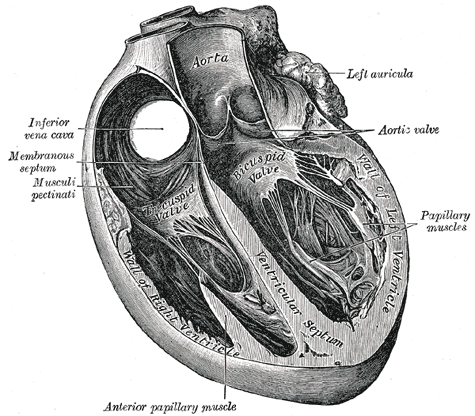
\includegraphics[width=0.7\textwidth]{figures/sample/Gray498.png} 
\caption[Four-chamber illustration of the human heart.]{Four-chamber illustration of the human heart.  Clockwise from upper-left: right atrium, left atrium, left ventricle, right ventricle.}
\label{fig:fourchamber}\end{figure}

The use of acoustic waves for medical diagnosis, inspired by naval sonar, was initially developed in the 1940s \cite{gagliardi_ultrasonography_1996}.  By 1954, the first clinically useful cardiac ultrasound -- examining motion of the mitral valve in stenosis -- was reported \cite{edler_ultrasonic_1957}.  These early scans were one-dimensional images (`A-mode'), sometimes repeated to generate a time axis (`M-mode').   The sector-scanning probe was developed in the 1970s \cite{bom_ultrasonic_1971,griffith_sector_1974}, leading to the `B-mode' that a modern cardiologist would recognise as an echocardiogram.


\chapter{Introduction}
\label{ch:introduction}
%
%	- objects are important and occur in many applications
%   - many models learn about objets only implicitly

	Our natural environments are filled with objects, and we interact with objects all the time: when driving a car, we need to think about other cars and pedestrians; opening a door often requires using a key.
	Objects are inherently of interest to us, and what follows is that they are also of interest to computer vision and machine learning communities.
	While there exists a vast body of literature on object detection and tracking (see\eg \cite{Liu2018deepod,Ciaparrone2019deepmot} for respective reviews), these two problems are typically solved using enormous amounts of human-labelled data. 
	The resulting models allow locating objects in images and tracking them in videos, but offer no further information about object behaviour, its intent, or its relationship with the environment and other objects.
	It is possibly for this reason that the majority of machine learning models for other tasks reported in the literature do not explicitly rely on object detection or tracking.
	Instead, these models treat objects only implicitly and gain knowledge about objects as a by-product of solving the main task, which can be playing Atari games \citep{Mnih2013dqn}, visual question answering \citep{Malinowski2015vqn}, image captioning \citep{Xu2015show}, or many others.
	Meanwhile, it has been verified that having disentangled representations\footnote{That is, representations in which different parts of the representation vector encode different factors of variation present in the dataset.} of the scene can lead to faster learning and better performance \citep{Steenkiste2019disentangled}.
	Similarly, having explicit representations of different objects in the scene---a kind of disentanglement---can lead to faster learning and more accurate predictive models \citep{Veerapaneni2019op3}. 
 	Explicit object representations can also be used with relational reasoning modules, and therefore improve results on a wide variety of tasks ranging from comparing objects \citep{Santoro2017} to learning to use tools \citep{Baker2019tooluse}.
 	Interestingly, we also know that humans (and other mammals) can learn about objects without any supervision \citep{Lambert2017cows}, contrary to current approaches to detection and tracking.
 	Given the above findings, it is natural to ask whether it is possible to build a machine learning system that learns about objects from vision inputs and without human supervision, and ideally one that can provide more information about objects than just their location.
 	Trying to answer this question is the main subject of this thesis.
 
    A very related question is that of ``what is an object?''.
    While we have no clear answer in sight, the works presented in this thesis can be seen as different attempts at finding an empirical definition of what an object might be.
    We revisit this question at the end of this thesis, in \Cref{sec:what_are_objects}, where we try to delve deeper into the nature of objects in images and videos.
 	
 	In order to answer this question, we begin by reviewing the existing literature in \Cref{ch:lit_review}. 
 	Since the subject of learning object-centric representations overlaps with
 		(1) relational reasoning,
 		(2) object detection and tracking,
 		(3) representation learning and disentanglement, and
 		(4) generative modelling, we devote separate sections to each of these areas. 
	Moreover, each of the following chapters, that is \Cref{ch:hart,ch:mohart,ch:sqair,ch:sca} contain additional related work sections that investigate literature that is most relevant to each of the respective chapters.
 	
 	Specifically, we start the overview of related works in \Cref{ch:lit_review} by reviewing relational reasoning algorithms, where we discuss pros and cons of different methods, and show that these methods rely on having access to some description of entities of interest,\eg ground-truth object state.
 	If that description is not available explicitly, it is often provided by a heuristic which can lead to sub-optimal results and increased computational cost.
 	We then change our focus to object detection and tracking algorithms, which could, in principle, be used to provide entity descriptions for relational reasoning. In practice this is not the case, however---even though these approaches can provide the object location and sometimes their class, they typically do not estimate object state\footnote{State can have a very broad meaning. What we mean here is a sufficient statistic of the object's future behaviour conditioned on the environment, or an internal Markovian state of that object, if such a state exists.} and therefore cannot provide any additional information about the detected or tracked objects.
 	This could still be better than using heuristic approaches but is far from using the ground-truth object state.
 	Next, we survey representation learning and disentangled representations literature.
 	The goal of representation learning is to learn to encode an input into a low-dimensional variable that contains relevant information about that input.
 	If this representation is disentangled, then using such a variable in downstream tasks can be much easier and more interpretable.
 	Under some circumstances, different objects could be described by different parts of that variable, which would constitute object-centric representations.
 	We show, however, that the community is interested in disentangling properties describing visual scenes in general, without particular focus on objects.
 	Finally, we turn to generative models, and show that the majority of approaches do not focus on representation learning, but there are some that do, and they sometimes use object-centric representations.
 	 
 	Having talked about the relevant literature, we go back to our original question. 
 	We begin by simplifying it and asking what does it take to learn object representations end-to-end, but with using supervision?
	\Cref{ch:hart} describes \textsc{HART}---a biologically-inspired single-object tracking algorithm, which uses two-stream processing and a hierarchy of attention mechanisms to single out the tracked object from its surroundings. 
	More specifically, it employs a \gls{RNN} to predict how the position and appearance of the object is going to change in the next time-step. 
	This knowledge enables extracting a small \textit{attention glimpse} that is likely to contain the object, as well as extracting the relevant features from this glimpse using a top-down attention mechanism.
	To solve this task, the state of the \gls{RNN} has to contain information about the object motion, its appearance, and its interactions with the environment, and meets the requirements of an object-centric representation.
	
 	While tracking single objects might be enough in some scenarios, it is often desirable to track multiple objects at the same time.
 	In \Cref{ch:mohart} we extend \textsc{hart} to multiple object tracking.
 	To do so, we run multiple trackers in parallel and use a self-attention mechanism to facilitate communication between the trackers. This approach achieves better tracking performance in the presence of global motion (\!\eg when the camera moves), when objects occlude each other or when they affect each others' trajectory---for example to avoid collisions. 
 	
 	In \Cref{ch:sqair} we go back to the original question, and build a system capable of generative modelling of multiple moving objects, which is learnt without any human supervision. 
 	Using this system, we can detect and track objects as well as predict their future trajectories. 
 	We apply it to videos from static \textsc{cctv} cameras, where it allows to detect and track pedestrians without supervision.
 
  	Finally, in \Cref{ch:sca} we build a deterministic generative model of images that has in-built knowledge of 2D geometry and can compose objects from their parts, and images from objects.
  	  This embedded knowledge allows it to learn what parts belong to which objects, and what are their typical geometric configurations.
  	    In some cases, this is sufficient for learning to classify objects without any supervision.
 	
 	\Cref{ch:discussion} discusses implications of our work and possible future research directions, as well as inherent limitations that approaches of this kind face. 
 	 It is worth noting that \Cref{ch:hart,ch:mohart,ch:sqair,ch:sca} are self-contained and based on the following publications:
 	 
   	\begin{enumerate}
        \item \fullcite{Kosiorek2017hierch},
        \item \fullcite{Fuchs2019mohart},
        \item \fullcite{Kosiorek2018sqair},
        \item \fullcite{Kosiorek2019stacked}.
 	\end{enumerate}
 	 
 	
 	\section{Works Omitted from the Thesis and Developed in the Course of This DPhil}

 	\begin{enumerate}
 	    \item \fullcite{Rainforth2018tighter}
 	    \item \fullcite{Le2019rrws}
 	    \item \fullcite{Lee2019set}
 	    \item \fullcite{Engelcke2019genesis}
 	    \item \fullcite{Fuchs2019stetho}
 	    \item \fullcite{Xu2019metafun}
 	    \item \fullcite{Dhir2017bayesian}
 	\end{enumerate}
 	
 	
 	
	
%	Typical machine learning use cases might involve (1) object detection and (2) tracking, (3) comparing objects with each other, (4) navigation in a cluttered environment, and (5) tool use \addref.
%	
%	Given how often reasoning about objects occurs in machine learning applications, one could think that there exist myriad models dealing with objects explicitly, and that objects might even be a structural component in many of these models.
%	
%	This is, however, not the case, and objects are usually neglected.
%	As an example, consider the three following applications: (1) learning to play Atari games \citep{dqn}, (2) visual question answering \citep{na}, and (3) image captioning \citep{image_caption}. 
%	Each of these applications requires learning about objects:\eg it is impossible to play Pong without knowing there the pads and the ball are, and it is difficult to describe an image without knowing what objects it contains.
%	Despite this, models used for these tasks are comprised of a \gls{CNN} followed by either a fully-connected or a recurrent network neural network, and are not structured at all\footnote{What we mean by structure here is similar to a structure of a graphical model, where all variables and dependencies between them are explicit.}.
%	It follows that objects have to be represented implicitly in these models.
%	Acquiring such implicit representations might be  computationally expensive in the sense that it might take many training cycles before such representations emerge. 
%	Additionally, a significant part of the model might be devoted to extracting those representations. 
%	In contrast, a structured model that describes objects explicitly might be smaller and could be trained faster.
%	Such a model would still have to learn how to use such representations, but we conjecture that this is an easier task, as suggested by the relevant literature \addref.
%	
%	Therefore, in this work we propose adding a structure to a typical deep learning model.
%	The typical model consists of a black-box neural network that consumes input (data) and produces output (answers), as shown in \Cref{fig:basic_arch}.
%	Instead, we suggest splitting this neural network into two components: (a) object representations, and (b) relational reasoning, cf.\ \Cref{fig:object_arch}. 
%	The first part should be able to parse the input and extract information about objects from it, ideally describing every object by a separate vector-valued variable\footnote{It should also encode information about the context.}.
%	The second part can then reason about objects and their context explicitly, and produce the desired output.
%	
%	Before diving into specifics of these two blocks, it is interesting to see an example of an application where such structure can be helpful.
%	
%	describe openai hide and seek
%	
%	The above example uses the proposed general architecture, with an important twist.
%	That is, instead of learning object-centric representations, the agents have access to the ground-truth state of the simulator.
%	While this is probably the best possible description of the objects, it is also out of reach in the majority of tasks where we simply have no access to their ground-truth state.
%	In practice, one has to infer object state from observations.
%	Unfortunately, the literature on this topic is rather sparse, with the notable exceptions of \cite{Greff2016tagger,Greff2017neuralem,Burgess2019monet,Eslami2016air}, as well as the work described in this thesis.
%	Relational reasoning, on the other hand, has been widely considered in recent literature, and there are many approaches for it, including relational networks \citep{Santoro2017}, self-attention \citep{Vaswani17,Lee2019set}, and graph neural networks \citep{gnns}.
%	For this reason we do not discuss relational reasoning approaches, and leave the choice of an appropriate method to practitioners.
%	
	
\chapter{Literature Review}
\label{ch:lit_review}

	Learning object-centric representations lies at the intersection of several areas of machine learning research. 
	Concretely, these are \begin{inparaenum}[(1)\!]
	\item relational reasoning, because having representations of objects can facilitate reasoning about their relations, but also because we can discover objects by analysing relations between different elements of a visual scene,
	\item object detection and tracking, as these two areas of research focus on locating objects in images and videos, respectively,
	\item representation learning, since the objective of our task it to learn representations, albeit ones that describe objects and not entire scenes, and finally
	\item compositional generative modelling, because object-centric representations can be useful for this task, but also because this area of research is among the most-promising candidates for learning object-centric representations.
	\end{inparaenum}
	We now describe these four areas in their dedicated sections, starting with relational reasoning.


\section{Relational Reasoning}
\label{sec:relational_reasoning}

	We define relational reasoning as making inferences about a group of entities such as physical objects with certain properties (\!\eg shape, mass) that exist in a shared context.
	 Importantly, we can make inferences about relations between any objects in a group, or we can use the knowledge of such relations to answer other (externally-posed) questions about the entities\footnote{Note that such answer can depend on the shared context, which can affect how objects relate to each other.}.
	 This definition closely follows that of \ak{fix this reference to be Battaglia et.\ al.} \cite{Battaglia2018relnets}, who also present an overview of this field of research. 
	 A typical example of relational reasoning is that of inferring which object in a scene is the biggest, or counting all objects made of metal \citep{Santoro2017}.
	 In a more complicated example, agents can learn the relations between objects in the environment, and use some objects to indirectly interact with other objects, which constitutes tool use \citep{Baker2019tooluse}.
	 If the existence and/or type of relations between objects are known, one can use this knowledge to build a \gls{GNN} \citep{Schlichtkrull2017relgraph} whose structure reflects these relations, and where different types of relations can be processed by dedicated neural modules.
	 If the number of entities is too large, or if relations only between neighbouring entities are known, one can process the graph of entities iteratively using message passing.
	 Alternatively, especially if relations between all objects exist or if their nature is not known, one could consider self-attention \citep{Vaswani17}, which performs relational reasoning on a fully-connected graph of entities.
	 The downside is the quadratic computational complexity (in the number of entities) of this approach.
	 Fortunately, this can be improved to linear computational complexity by using inducing points \citep{Lee2019set} or local self-attention \citep{Ramachandran2019standalone}.
	 
	 Relational reasoning can be useful for inferring which parts of the scene constitute objects, but in order to reason about relations, one has to know what entities are present in the scene. 
	 Typically, this data is not available and one has to resort to heuristic solutions.
	 \cite{Santoro2017} use a \gls{CNN} to embed an image into a feature map and assumes that each location in this feature map can correspond to an object. 
	 They then consider pairwise relations between every pair of locations.
	 \cite{Battaglia2016,Baker2019tooluse} assume access to the ground-truth state of different entities,
	 and \cite{Yi2019cleverer} use \textsc{mask r-cnn} \citep{He2017maskrcnn} for segmenting out different objects before feeding them into a relational reasoning module.
	 More generally, one can use any object detection, segmentation, or region proposal\footnote{Regions of interest need not correspond to objects.} algorithm to identify \textit{interesting} parts of the scene and supply information about their whereabouts and appearance to a relational reasoning module.
	 In the context of timeseries, it is useful to know temporal characteristics of objects, which can be provided by object tracking algorithms.
	 Therefore, we now discuss object detection and tracking methods, and their suitability for relational reasoning applications.
	 
\section{Object Detection and Tracking}
\label{sec:object_det_track}

	Object detection and tracking have been of long-standing interest to the computer vision community, with early works that appeared in XXX and YYY, respecitvely \addref.
	Both problems are typically addressed in a supervised manner, where object bounding boxes and/or segmentation masks and often additional labels are provided as a part of the training data.
	\paragraph{Object detection}
	rcnn family of the models as SOTA
	
	\paragraph{Object tracking}
	Object tracking is typically initialised with an object bounding box (either ground-truth or from a detector) and can be divided into two broad categories of long- or short-term single-object tracking and multi-object tracking.
	In short-term tracking, the algorithm is not provided with further detections, while in long-term tracking it typically has access to external detections and can restart in case of a failure.
	
%	
%
	\textbf{Single-object tracking} commonly uses Siamese networks \citep{Valmadre2017,Held2016goturn}, first introduced in \citep{Bromley1993siamese}.
	These approaches typically work by comparing a source patch containing the object of interest to patches at several locations in the target image.
	The highest-scoring patch in the target image is deemed to match the source patch, and its centre is taken as the new position of the tracked object.
	In order to handle scale differences, the source patch is compared to the target image at several different scales.
	Instead of comparing it to the whole target image, one typically constrains the region of interest to an area around the last known location of the object.
	Sometimes simple motion models (\!\eg Kalman filter, \cite{Swerling1959kalman,Kalman1961kalman}) are used to further reduce the size of the search region.
	
	These types of algorithms can provide relational reasoning modules with a sequence of locations, but no other information is available.
	Similarly to object detection algorithms, one could use intermediate representation from one of the layers of a Siamese net as an input for relational reasoning.
	However, since these methods perform only appearance-based matching of source and target features, there is no guarantee for these features to contain any useful information\eg about appearance changes.
	Moreover, since these methods do not aggregate information through time, they are unable to inform about object intent or its motion.
	This is in contrast to end-to-end tracking approaches, where models do estimate object state and learn to anticipate position and appearance changes.
	More specifically, Siamese networks can be seen as an \gls{RNN} unrolled over two time-steps.
	Recently, we used an \gls{RNN} with an attention mechanism in the \textsc{hart} model (\Cref{ch:hart}) to predict bounding boxes for single objects, while robustly modelling their motion and appearance.
	\textsc{Hart} is based on \textsc{ratm} \citep{Kahou2015ratm}, but decouples attention and bounding-box prediction and features an additional attention mechanism.
	At the time, \textsc{hart} was the best-performing \gls{RNN}-based tracker, outperfomed only by the concurrently developed \textsc{re3} of \cite{Gordon2018re3}, which is also based on an \gls{RNN}, but is not end-to-end due to the use of hard attention for cropping.
	\textsc{Hart} was extended to handle \textsc{rgbd} inputs in \cite{Danesh2019deep}. 
	It was also augmented with a meta-learning update to better remember the tracked object in \cite{Li2019metahart}. We also extended it to multi-object tracking in \Cref{ch:mohart}, which is discussed further below.
	
%	
%
	\textbf{Multi-object tracking} is typically attained by detecting objects and performing data association on bounding-boxes in order to link them into coherent trajectories \citep{Zhang2008,Milan2014,Bae2017confidence,Keuper2018motion}, which differs considerably from the single-object tracking paradigm.
	Many approaches additionally use motion models and appearance to improve data association, see\eg \cite{Bewley2016sort}.
	While recent approaches replace some steps of this method with learned elements \citep{Schulter2017deepnf,Nam2016,Ning2017,Keuper2018motion,Bae2017confidence,Xiang2015}, no truly end-to-end multi-object tracking method exists, with the exception of unsupervised video-modelling models described in \Cref{sec:gen_modelling} and including \textsc{sqair} of \Cref{ch:sqair}.
	
%	\textbf{Discussion}
%	Object detection and tracking algorithms can provide valuable information that can be used as input to relational reasoning algorithms, but the extracted information is typically limited to the the location and possibly the history of object locations.
%	Given the location, it is possible to extract information about appearance and possibly other characteristics, but this requires complicated post-processing.
	
%	\cite{Schulter2017deepnf} used an end-to-end supervised approach that detects objects and performs data association.
%	In the unsupervised setting, where the training data consists of only images or videos, the dominant approach is to distill the inductive bias of spatial consistency into a discriminative model.  \cite{Cho2015unsupervised} detect single objects and their parts in images, and \cite{Kwak2015unsupervised,Xiao2016track} incorporate temporal consistency to better track single objects.
%	\Gls{SQAIR} is unsupervised and hence it does not rely on bounding boxes nor additional labels for training, while being able to learn arbitrary motion and appearance models similarly to \textsc{hart} \citep{Kosiorek2017hierch}.
%	At the same time, is inherently multi-object and performs data association implicitly (\textit{cf}. \Cref{app:algo}).
%	Unlike the other unsupervised approaches, temporal consistency is baked into the model structure of \gls{SQAIR} and further enforced by lower \gls{KL} divergence when an object is tracked.
	
%	\paragraph{End-to-End Tracking} A newly established and much less explored stream of work approaches tracking in an end-to-end fashion. A key difficulty here is that extracting an image crop (according to bounding-boxes provided by a detector), is non-differentiable and results in high-variance gradient estimators.
%	\citet{Kahou2015ratm} propose an end-to-end tracker with soft spatial-attention using a 2D grid of Gaussians instead of a hard bounding-box. \Gls{HART} draws inspiration from this idea, employs an additional attention mechanism, and shows promising performance on the real-world KITTI dataset \cite{Kosiorek2017hierch}.
%	\Gls{HART}, which forms the foundation of this work, is explained in detail in \Cref{sec:method}. It has also been extended to incorporate depth information from \textsc{rgbd} cameras \cite{Danesh2019deep}. \citet{Gordon2018re3} propose an approach in which the crop corresponds to the scaled up previous bounding-box. This simplifies the approach, but does not allow the model to learn where to look---\ie no gradient is backpropagated through crop coordinates.
%	To the best of our knowledge, there are no successful implementations of any such end-to-end approaches for multi-object tracking beyond \textsc{sqair} \citep{Kosiorek2018sqair}, which works only on datasets with static backgrounds. On real-world data, the only end-to-end approaches correspond to applying multiple single-object trackers in parallel---a method which does not leverage the potential of scene context or inter-object interactions. 
	


\section{Representation Learning and Disentanglement}
\label{sec:repr_learning}


		[Learning Decomposed Representations of Images and Videos]
	Learning decomposed representations of object appearance and position lies at the heart of our model.
	This problem can be also seen as perceptual grouping, which involves modelling pixels as spatial mixtures of entities.
	\cite{Greff2016tagger} and \cite{Greff2017neuralem} learn to decompose images into separate entities by iterative refinement of spatial clusters using either learned updates or the Expectation Maximization algorithm;
	\cite{Ilin2017recurrentln} and \cite{Steenkiste2018} extend these approaches to videos, achieving very similar results to \gls{SQAIR}.
	Perhaps the most similar work to ours is the concurrently developed model of \cite{Hsieh2018ddpae}.
	The above approaches rely on iterative inference procedures, but do not exhibit the object-counting behaviour of \gls{SQAIR}.
	For this reason, their computational complexities are proportional to the predefined maximum number of objects, while \gls{SQAIR} can be more computationally efficient by adapting to the number of objects currently present in an image.
	
	Another interesting line of work is the \textsc{gan}-based unsupervised video generation that decomposes motion and content \citep{Tulyakov2017mocogan,Denton2017unsupervised}. These methods learn interpretable features of content and motion, but deal only with single objects and do not explicitly model their locations. Nonetheless, adversarial approaches to learning structured probabilistic models of objects offer a plausible alternative direction of research.



\section{Generative Modelling}
\label{sec:gen_modelling}

	There are two main approaches to unsupervised object category detection in computer vision.
	The first one is based on representation learning and typically requires discovering clusters or learning a classifier on top of the learned representation.
	\cite{Eslami2016air,Kosiorek2018sqair} use an iterative procedure to infer a variable number of latent variables, one for every object in a scene, that are highly informative of object class, while \cite{Greff2019multi,Burgess2019monet} perform unsupervised instance-level segmentation in an iterative fashion.
	While similar to our work, these approaches cannot decompose objects into their constituent parts and do not provide explicit description of object shape (\!\eg templates and their poses in our model).
	
	The second approach targets classification explicitly by minimizing mutual information (\textsc{mi})-based losses and directly learning class-assignment probabilities.
	\textsc{Iic} \citep{Ji2018iic} maximizes an exact estimator of \textsc{mi} between two discrete probability vectors describing (transformed) versions of the input image.
	DeepInfoMax \citep{Hjelm2019deepinfomax} relies on negative samples and maximizes \textsc{mi} between the predicted probability vector and its input via noise-contrastive estimation \citep{Gutmann2010nce}.
	This class of methods directly maximizes the amount of information contained in an assignment to discrete clusters and they hold state-of-the-art results on most unsupervised classification tasks.
	\textsc{Mi}-based methods suffer from typical drawbacks of mutual information estimation: they require heavy data augmentation and large batch sizes.
	This is in contrast to our method, which achieves comparable performance with batch size no bigger than 128 and with no data augmentation.
	
	
	
	[Video Prediction]
	Many works on video prediction learn a deterministic model conditioned on the current frame to predict the future ones \citep{Ranzato2014video,Srivastava2015unsupervised}.
	Since these models do not model uncertainty in the prediction, they can suffer from the multiple futures problem --- since perfect prediction is impossible, the model produces blurry predictions which are a mean of possible outcomes.
	This is addressed in stochastic latent variable models trained using variational inference to generate multiple plausible videos given a sequence of images \citep{Babaeizadeh2017stochastic, Denton2018stochastic}.
	Unlike \gls{SQAIR}, these approaches do not model objects or their positions explicitly, thus the representations they learn are of limited interpretability. 
	


%\textbf{Capsule Networks}\ \ 
%Our work combines ideas from Transforming Autoencoders \citep{Hinton2011tae} and \textsc{em} Capsules \citep{Hinton2018capsule}.
%Transforming autoencoders discover affine-aware capsule \textit{instantiation parameters} by training an autoencoder to predict an affine-transformed version of the input image from the original image plus an extra input, which explicitly represents the transformation.
%By contrast, our model does not need any input other than the image.
%
%Both \textsc{em} Capsules and the preceding Dynamic Capsules \citep{Sabour2017capsule} use the poses of parts and learned part$\rightarrow$object relationships to vote for the poses of objects. When multiple parts cast very similar votes, the object is assumed to be present, which is facilitated by an interactive inference (routing) algorithm. Iterative routing is inefficient and has prompted further research. \cite{Wang2018optimization} formulated routing as an optimization of a clustering loss and a \textsc{kl}-divergence-based regularization term.  \cite{Zhang2018fast} proposed a weighted kernel density estimation-based routing method. \cite{Li2018encapsule} proposed approximating routing with two branches and sending feedback via optimal transport divergence between two distributions (lower and higher capsules). 
%In contrast to prior work, we use objects to predicts parts rather than vice-versa, therefore we can dispense with iterative routing at inference time. The encoder of the \gls{OCAu} learns how to group parts into objects and it respects the single parent constraint, because it is trained using derivatives produced by a decoder that uses a mixture model of parts which assumes that each part must be explained by a single object. 
%
%Additionally, since it is the objects that predict parts, the parts are allowed to have fewer degrees-of-freedom in their poses than objects (as in the \gls{CCAu}). 
%Inference is still possible, because the \gls{OCAu} encoder makes object predictions based on {\it all} the parts rather than an individual part.
%
%A further advantage of our version of capsules is that it can perform unsupervised learning. Previous versions of capsules used discriminative learning, though \cite{Rawlinson2018sparsecaps} used the reconstruction \gls{MLP} introduced in \cite{Sabour2017capsule} to train Dynamic Capsules without supervision and has shown that unsupervised training for capsule-conditioned reconstruction helps with generalization to \textsc{affnist} classification; we further improve on their results, \textit{cf}.\ \Cref{sec:ablation}.

%
%%spatial attention
%A number of recent studies have demonstrated that visual content can be captured through a sequence of spatial glimpses or foveation \cite{Graves2014recurrent, Gregor2016towards}. Such a paradigm has the intriguing property that the computational complexity is proportional to the number of steps as opposed to the image size.
%Furthermore, the fovea centralis in the retina of primates is structured with maximum visual acuity in the centre and decaying resolution towards the periphery, \citet{Olshausen2016foveal} show that if spatial attention is capable of zooming, a regular grid sampling is sufficient. 
%\citet{Jaderberg2015} introduced the spatial transformer network (STN) which provides a fully differentiable means of transforming feature maps, conditioned on the input itself. \citet{Eslami2016air} use the STN as a form of attention in combination with a recurrent neural network (RNN) to sequentially locate and identify objects in an image. Moreover, \citet{Eslami2016air} use a latent variable to estimate the presence of additional objects, allowing the RNN to adapt the number of time-steps based on the input. 
%Our spatial attention mechanism is based on the two dimensional Gaussian grid filters of  \cite{Kahou2015ratm} which is both fully differentiable and more biologically plausible than the STN.  
%%While the aforementioned approaches use a regular sampling lattice which is far simpler than of the primate retina, \citet{Olshausen2016foveal} showed that complex sampling patterns are not required when attention is able to zoom-in on a region of interest. 
%
%%appearance attention with RNNs
%Whilst focusing on a specific location has its merits, focusing on particular appearance features might be as important. A policy with feedback connections can learn to adjust filters of a convolutional neural network (CNN), thereby adapting them to features present in the current image and improving accuracy \cite{Stollenga2014}. \citet{Brabandere2016dfn} introduced dynamic filter network (DFN), where filters for a CNN are computed on-the-fly conditioned on input features, which can reduce model size without performance loss. \citet{Karl2017dvbf} showed that an input-dependent state transitions can be helpful for learning latent Markovian state-space system. While not the focus of this work, we follow this concept in estimating the expected appearance of the tracked object.



\chapter{Hierarchical Attentive Recurrent Tracking}
\label{ch:hart}
\chapter{Hierarchical Attentive Recurrent Tracking}

\begin{abstract}
  Class-agnostic object tracking is particularly difficult in cluttered environments as target specific discriminative models cannot be learned \emph{a priori}. Inspired by how the human visual cortex employs spatial attention and separate ``where'' and ``what'' processing pathways to actively suppress irrelevant visual features, this work develops a hierarchical attentive recurrent model for single object tracking in videos. The first layer of attention discards the majority of background by selecting a region containing the object of interest, while the subsequent layers tune in on visual features \emph{particular} to the tracked object. 
  This framework is fully differentiable and can be trained in a purely data driven fashion by gradient methods. To improve training convergence, we augment the loss function with terms for auxiliary tasks relevant for tracking. Evaluation of the proposed model is performed on two datasets: pedestrian tracking on the KTH activity recognition dataset and the more difficult KITTI object tracking dataset.
\end{abstract}
 
    In computer vision, designing an algorithm for model-free tracking of anonymous objects is challenging, since no target-specific information can be gathered \emph{a priori} and yet the algorithm has to handle target appearance changes, varying lighting conditions and occlusion. 
    To make it even more difficult, the tracked object often constitutes but a small fraction of the visual field. 
    The remaining parts may contain \emph{distractors}, which are visually salient objects resembling the target but hold no relevant information. 
    Despite this fact, recent models often process the whole image,
    which exposes them to noise
    and increases the associated computational cost or they use heuristic methods to decrease the size of search regions. 
    This in contrast to human visual perception, which does not process the visual field in its entirety, but rather acknowledges it briefly and focuses on processing small fractions thereof, which we dub \emph{visual attention}.
    
\begin{figure}[ht!]
	\centering
	\begin{minipage}[c]{0.67\textwidth}
		\centering
        \begin{subfigure}[b]{1.\textwidth}
      		 \centering
             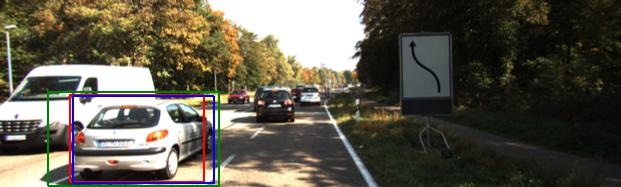
\includegraphics[width=\textwidth]{HART/att_img}
        \end{subfigure}
%        \hspace{-30pt}
        \begin{minipage}{.85\textwidth}
        	\centering
            \begin{subfigure}[b]{.29\textwidth}
                \sidecaption{fig:glimpse}
                \raisebox{-.5\height}{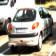
\includegraphics[width=\textwidth, cfbox=darkgreen 1pt 0pt]{HART/att_glimpse}}
            \end{subfigure}
            \hfill
            \hspace{8pt}
            \begin{subfigure}[b]{.29\textwidth}
                \sidecaption{fig:mask}
                \raisebox{-.5\height}{
\includegraphics[width=\textwidth]{HART/att_mask}}
            \end{subfigure}
            \hfill
            \hspace{5pt}
            \begin{subfigure}[b]{.29\textwidth}
                \sidecaption{fig:overlay}
                \raisebox{-.5\height}{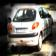
\includegraphics[width=\textwidth]{HART/att_overlay}}
            \end{subfigure}
        \end{minipage}
	\end{minipage}
	\begin{minipage}[c]{0.2\textwidth}
   		\caption{KITTI image with the \textcolor{blue}{ground-truth} and \textcolor{red}{predicted} bounding boxes and an \textcolor{darkgreen}{attention glimpse}. The lower row corresponds to the hierarchical attention of our model: $1^{st}$ layer extracts an attention glimpse (a), the $2^{nd}$ layer uses appearance attention to build a location map (b). The $3^{rd}$ layer uses the location map to suppress distractors, visualised in (c).}
        \label{fig:img_with_att}
	\end{minipage}
\end{figure}
    Attention mechanisms have recently been explored in machine learning in a wide variety of contexts \cite{Vinyals2014, Jaderberg2015}, often providing new capabilities to machine learning algorithms \cite{Graves2016dnc,Gregor2016towards, Eslami2016air}. While they improve efficiency \cite{Graves2014recurrent} and performance on state-of-the-art machine learning benchmarks \cite{Vinyals2014}, their architecture is much simpler than that of the mechanisms found in the human visual cortex \cite{Dayan2001}. Attention has also been long studied by neuroscientists \cite{Ungerleider2000}, who believe that it is crucial for visual perception and cognition \cite{Olshausen2016foveal}, since it is inherently tied to the architecture of the visual cortex and can affect the information flow inside it. Whenever more than one visual stimulus is present in the receptive field of a neuron, all the stimuli compete for computational resources due to the limited processing capacity. 
	%%% How attention is relevant to tracking in cv
	% 	Types of attention
	Visual attention can lead to suppression of distractors by reducing the size of the receptive field of a neuron and by increasing sensitivity at a given location in the visual field (\emph{spatial attention}). It can also amplify activity in different parts of the cortex, which are
	specialised in processing different types of features, leading to  response enhancement with respect to those features (\emph{appearance attention}).
% 	Distinct pathways
	The functional separation of the visual cortex is most apparent in two distinct processing pathways. After leaving the eye, the sensory inputs enter the primary visual cortex (known as \emph{V1}) and then split into the \emph{dorsal stream}, responsible for estimating spatial relationships (\emph{where}), and the \emph{ventral stream}, which targets appearance-based features (\emph{what}).

    Inspired by the general architecture of the human visual cortex and the role of attention mechanisms, this work presents a biologically-inspired recurrent model for single object tracking in videos (\emph{cf.} \cref{sec:att}). Tracking algorithms typically use simple motion models and heuristics to decrease the size of the search region. It is interesting to see whether neuroscientific insights can aid our computational efforts, thereby improving the efficiency and performance of single object tracking.
    % 	Inspired by the general architecture of the human visual cortex and the role of attention mechanisms, this work presents a biologically-inspired recurrent model for single object tracking in videos (\emph{cf.} \cref{sec:att}).
	% 	Different sources of attention
	It is worth noting that visual attention can be induced by the stimulus itself (due to, \eg high contrast) in a \emph{bottom-up} fashion or by back-projections from other brain regions and working memory as \emph{top-down} influence. The proposed approach exploits this property to create a feedback loop that steers the \emph{three} layers of visual attention mechanisms in our hierarchical attentive recurrent tracking (\emph{HART}) framework, see \Cref{fig:img_with_att}. The first stage immediately discards spatially irrelevant input, while later stages focus on producing target-specific filters to emphasise visual features \emph{particular} to the object of interest.
	
% 	By factoring the problem into its constituent parts, we arrive at a familiar statistical domain; namely that of maximum likelihood estimation (MLE). 
    The resulting framework is end-to-end trainable and we resort to maximum likelihood estimation (MLE) for parameter learning.
	This follows from our interest in estimating the distribution over object locations in a sequence of images, given the initial location from whence our tracking commenced. 
	Formally, given a sequence of images $\bxTs \in \RR^{H \times W \times C}$, where the superscript denotes height, width and the number of channels of the image, respectively, and an initial location for the tracked object given by a bounding box $\bb_1 \in \RR^4$, the conditional probability distribution factorises as
    \begin{equation}
        \p{\bb_{2:T}}{\bxTs, \bb_1} = \int \p{\B{h}_1}{\bx_1, \bb_1} \prod_{t=2}^T \int \p{\bbt}{\B{h}_t} \p{\B{h}_t}{\bxt, \bb_{t-1}, \B{h}_{t-1}} \dint \B{h}_t \dint \B{h}_1,
    \end{equation}
    where we assume that motion of an object can be described by a Markovian state $\B{h}_t$.
    Our bounding box estimates are given by $\widehat{\bb}_{2:T}$, found by the MLE of the model parameters. In sum, our contributions are threefold: 
    Firstly, a hierarchy of attention mechanisms that leads to suppressing distractors and computational efficiency is introduced.
    Secondly, a biologically plausible combination of attention mechanisms and recurrent neural networks is presented for object tracking.
    Finally, our attention-based tracker is demonstrated using real-world sequences in challenging scenarios where previous recurrent attentive trackers have failed.
    \iffalse
    \begin{itemize}
        \item a biologically plausible way of combining attention mechanisms with recurrent neural networks for object tracking,
        \item a hierarchy of attention mechanisms that leads to suppressing distractors and computational efficiency,
        \item the scaling of an attention-based tracker to real-world exceeding prior recurrent attentive tracking models. 
    \end{itemize}
    \fi
    Next we briefly review related work (\Cref{sec:background}) before describing how information flows through the components of our hierarchical attention in \Cref{sec:att}. \Cref{sec:loss} details the losses applied to guide the attention. \Cref{sec:exp} presents experiments on KTH and KITTI datasets with comparison to related attention-based trackers. \Cref{sec:hart_discussion} discusses the results and intriguing properties of our framework and \Cref{sec:conclusion} concludes the work. Code and results are available online\footnote{\url{https://github.com/akosiorek/hart}}.
        

	
	
	
	
	
	
	
	
	

	

\section{Related Work}
\label{sec:background}

%spatial attention
A number of recent studies have demonstrated that visual content can be captured through a sequence of spatial glimpses or foveation \cite{Graves2014recurrent, Wierstra2015draw}. Such a paradigm has the intriguing property that the computational complexity is proportional to the number of steps as opposed to the image size.
Furthermore, the fovea centralis in the retina of primates is structured with maximum visual acuity in the centre and decaying resolution towards the periphery, \citet{Olshausen2016foveal} show that if spatial attention is capable of zooming, a regular grid sampling is sufficient. 
\citet{Jaderberg2015} introduced the spatial transformer network (STN) which provides a fully differentiable means of transforming feature maps, conditioned on the input itself. \citet{Eslami2016} use the STN as a form of attention in combination with a recurrent neural network (RNN) to sequentially locate and identify objects in an image. Moreover, \citet{Eslami2016} use a latent variable to estimate the presence of additional objects, allowing the RNN to adapt the number of time-steps based on the input. 
Our spatial attention mechanism is based on the two dimensional Gaussian grid filters of  \cite{Kahou2015ratm} which is both fully differentiable and more biologically plausible than the STN.  
%While the aforementioned approaches use a regular sampling lattice which is far simpler than of the primate retina, \citet{Olshausen2016foveal} showed that complex sampling patterns are not required when attention is able to zoom-in on a region of interest. 


    
%appearance attention with RNNs
Whilst focusing on a specific location has its merits, focusing on particular appearance features might be as important. A policy with feedback connections can learn to adjust filters of a convolutional neural network (CNN), thereby adapting them to features present in the current image and improving accuracy \cite{Stollenga2014}. \citet{Brabandere2016dfn} introduced dynamic filter network (DFN), where filters for a CNN are computed on-the-fly conditioned on input features, which can reduce model size without performance loss. \citet{Karl2017} showed that an input-dependent state transitions can be helpful for learning latent Markovian state-space system. While not the focus of this work, we follow this concept in estimating the expected appearance of the tracked object.
    
%attention in tracking  
In the context of single object tracking, both attention mechanisms and RNNs appear to be perfectly suited, yet their success has mostly been limited to simple monochromatic sequences with plain backgrounds \cite{Kahou2015ratm}. \citet{Cheung2016gtc} applied STNs \cite{Jaderberg2015} as attention mechanisms for real-world object tracking, but failed due to exploding gradients potentially arising from the difficulty of the data.
\citet{Ning2016} achieved competitive performance by using features from an object detector as inputs to a long-short memory network (LSTM), but requires processing of the whole image at each time-step. 

Two recent state-of-the-art trackers employ convolutional Siamese networks which can be seen as an RNN unrolled over two time-steps \cite{Held2016, Valmadre2017}. Both methods explicitly process small search areas around the previous target position to produce a bounding box offset \cite{Held2016} or a correlation response map with the maximum corresponding to the target position \cite{Valmadre2017}. 
We acknowledge the recent work\footnote{\cite{Gordon2017} only became available at the time of submitting this paper.} of \citet{Gordon2017} which employ an RNN based model and use explicit cropping and warping as a form of non-differentiable spatial attention.
The work presented in this paper is closest to \cite{Kahou2015ratm} where we share a similar spatial attention mechanism which is guided through an RNN to effectively learn a motion model that spans multiple time-steps. The next section describes our additional attention mechanisms in relation to their biological counterparts.



    
    

\section{Hierarchical Attention}
\label{sec:att}

    % \begin{enumerate}
    %     \item Hierarchy; refer to the figure, give overview; explain the terms
    %     \item Spatial Attention; short; it's not novel but requires restating; it's important to have one followed by the other
    %     \item Appearance Attention; DFN
    %     \item Highlight the hierarchy; recurrence reinforces it even further
    % \end{enumerate}

	\begin{figure}[ht]
		\centering
	 	\usebox{\systemfig}
	 	\vspace{-2.5em}
	 	\caption{Hierarchical Attentive Recurrent Tracking. Spatial attention extracts a glimpse $\bgt$ from the input image $\bxt$. V1 and the ventral stream extract appearance-based features $\bmapt$ while the dorsal stream computes a foreground/background segmentation $\bst$ of the attention glimpse. Masked features $\bvt$ contribute to the working memory $\B{h}_t$. The LSTM output $\bot$ is then used to compute attention $\ba_{t+1}$, appearance $\bapp_{t+1}$ and a bounding box correction $\Delta \widehat{\bb}_t$. Dashed lines correspond to temporal connections, while solid lines describe information flow within one time-step.}
		\label{fig:system}
		\vspace{-.5em}
	\end{figure}
	
    \begin{figure}
      \begin{minipage}[c]{0.3\textwidth}
        \usebox{\archfig}
      \end{minipage}\hfill
      \begin{minipage}[c]{0.6\textwidth}
        \caption{Architecture of the appearance attention. V1 is implemented as a CNN shared among the dorsal stream (DFN) and the ventral stream (CNN). The $\odot$ symbol represents the Hadamard product and implements masking of visual features by the foreground/background segmentation.}
    	\label{fig:arch}
      \end{minipage}
      \vspace{-1.5em}
    \end{figure}

	Inspired by the architecture of the human visual cortex, we structure our system around working memory responsible for storing the motion pattern and an appearance description of the tracked object. If both quantities were known, it would be possible to compute the expected location of the object at the next time step. Given a new frame, however, it is not immediately apparent which visual features correspond to the appearance description. If we were to pass them on to an RNN, it would have to implicitly solve a data association problem. As it is non-trivial, we prefer to model it explicitly by outsourcing the computation to a separate processing stream conditioned on the expected appearance. This results in a location-map, making it possible to neglect features inconsistent with our memory of the tracked object. We now proceed with describing the information flow in our model.
	    
    % Inspired by the architecture of human visual cortex, we implement the hierarchical attention mechanism as follows (see the model in \cref{fig:system}). Given attention parameters $\bat$, the \emph{spatial attention} module extracts a glimpse $\bgt$ from the input image $\bxt$. We then apply \emph{appearance attention}, parametrised by appearance $\bappt$ and comprised of V1 and dorsal and ventral streams, to obtain object-specific features $\bvt$, which are used to update the hidden state $\B{h}_t$ of the LSTM. The LSTM's output is then decoded to predict both spatial and appearance attention parameters for the next time-step along with a bounding box correction $\Delta \widehat{\bb}_t$ for the current time-step.
    
    Given attention parameters $\bat$, the \emph{spatial attention} module extracts a glimpse $\bgt$ from the input image $\bxt$. We then apply \emph{appearance attention}, parametrised by appearance $\bappt$ and comprised of V1 and dorsal and ventral streams, to obtain object-specific features $\bvt$, which are used to update the hidden state $\B{h}_t$ of an LSTM. The LSTM's output is then decoded to predict both spatial and appearance attention parameters for the next time-step along with a bounding box correction $\Delta \widehat{\bb}_t$ for the current time-step.
    Spatial attention is driven by top-down signal $\bat$, while appearance attention depends on top-down $\bappt$ as well as bottom-up (contents of the glimpse $\bgt$) signals. Bottom-up signals have local influence and depend on stimulus salience at a given location, while top-down signals incorporate global context into local processing. This attention hierarchy, further enhanced by recurrent connections, mimics that of the human visual cortex \cite{Ungerleider2000}. We now describe the individual components of the system.
    
  \begin{description}[leftmargin=\parindent]
  \item[Spatial Attention]

	Our spatial attention mechanism is similar to the one used by \citet{Kahou2015ratm}. Given an input image $\bxt \in \RR^{H \times W}$, it creates two matrices $\bAt^x \in \RR^{w \times W}$ and $\bAt^y \in \RR^{h \times H}$, respectively. Each matrix contains one Gaussian per row; the width and positions of the Gaussians determine which parts of the image are extracted as the attention glimpse. Formally, the glimpse $\bgt \in \RR^{h \times w}$ is defined as
	\begin{equation}
		\bgt = \bAt^y \bxt \left( \bAt^x \right)^{\mathsf{T}}.
	\end{equation} 
	Attention is described by centres $\mu$ of the Gaussians, their variances $\sigma^2$ and strides $\gamma$ between centers of Gaussians of consecutive rows of the matrix, one for each axis. In contrast to the work by \citet{Kahou2015ratm}, only centres and strides are estimated from the hidden state of the LSTM, while the variance depends solely on the stride. This prevents excessive aliasing during training caused when predicting a small variance (compared to strides) leading to smoother convergence. The relationship between variance and stride is approximated using linear regression with polynomial basis functions (up to $4^{th}$ order) before training the whole system. The glimpse size we use depends on the experiment.
	% detail ->Linear regression was fitted before training the system, with the objective to approximate bicubic interpolation with the resulting attention glimpse. 	
	
  \item[Appearance Attention]

    This stage transforms the attention glimpse $\bgt$ into a fixed-dimensional vector $\bvt$ comprising appearance and spatial information about the tracked object. Its architecture depends on the experiment. In general, however, we implement $\mathrm{V1} : \RR^{h \times w} \to \RR^{h_v \times w_v \times c_v}$ as a number of convolutional and max-pooling layers. They are shared among later processing stages, which corresponds to the primary visual cortex in humans \cite{Dayan2001}. Processing then splits into ventral and dorsal streams. The ventral stream is implemented as a CNN, and handles visual features and outputs feature maps $\bmapt$. The dorsal stream, implemented as a DFN, is responsible for handling spatial relationships. Let $\MLP{\cdot}$ denote a multi-layered perceptron. The dorsal stream uses appearance $\bappt$ to dynamically compute convolutional filters $\bdparamt^{a \times b \times c \times d}$, where the superscript denotes the size of the filters and the number of input and output feature maps, as
 	\begin{equation}
 	    \B{\Psi}_t = \set{\bdparamt^{a_i \times b_i \times c_i \times d_i}}_{i=1}^{K} = \MLP{\bappt}.
 	\end{equation}
    The filters with corresponding nonlinearities form $K$ convolutional layers applied to the output of V1. Finally, a convolutional layer with a $1 \times 1$ kernel and a sigmoid non-linearity is applied to transform the output into a spatial Bernoulli distribution $\bst$. Each value in $\bst$ represents the probability of the tracked object occupying the corresponding location.
 
    The location map of the dorsal stream is combined with appearance-based features extracted by the ventral stream, to imitate the distractor-suppressing behaviour of the human brain. It also prevents drift  and allows occlusion handling, since object appearance is not overwritten in the hidden state when input does not contain features particular to the tracked object. Outputs of both streams are combined as\footnote{$\mathrm{vec}: \RR^{m \times n} \to \RR^{mn}$ is the vectorisation operator, which stacks columns of a matrix into a column vector.}
	\begin{equation}
		\bvt = \MLP{ \flatten{\bmapt \odot \bst}},
	\end{equation}
	with $\odot$ being the Hadamard product.
   
   
  \item[State Estimation]
    
    Our approach relies on being able to predict future object appearance and location, and therefore it heavily depends on state estimation. We use an LSTM, which can learn to trade-off spatio-temporal and appearance information in a data-driven fashion. It acts like a working memory, enabling the system to be robust to occlusions and oscillating object appearance \eg when an object rotates and comes back to the original orientation.
    \begin{equation} 
        \label{eq:state}
        % \mathrm{LSTM}: \bvt, \B{h}_{t-1} \mapsto \bot, \B{h}_t
    	\bot, \B{h}_t = \LSTM{ \bvt, \B{h}_{t-1} },
    \end{equation}
    \begin{equation} 
	    \label{eq:mlp}
	   % \mathrm{MLP}: \bot, \vec{\bst} \mapsto \bapp_{t+1}, \Delta \ba_{t+1}, \Delta \widehat{\bb}_t
	    \bapp_{t+1}, \Delta \ba_{t+1}, \Delta \widehat{\bb}_t = \MLP{ \bot, \flatten{\bst} },
    \end{equation}
    \begin{equation}
        \label{eq:att_update}
     	\ba_{t+1} = \bat + \tanh(\B{c}) \Delta \ba_{t+1},
    \end{equation}
    \begin{equation}
        \label{eq:bbox_update}
     	\widehat{\bb}_t = \bat + \Delta \widehat{\bb}_t
    \end{equation}
    \Cref{eq:state,eq:mlp,eq:att_update,eq:bbox_update} detail the state updates. Spatial attention at time $t$ is formed as a cumulative sum of attention updates from times $t=1$ to $t=T$, where $\B{c}$ is a learnable parameter initialised to a small value to constrain the size of the updates early in training. Since the spatial-attention mechanism is trained to predict where the object is going to go (\Cref{sec:loss}), the bounding box $\widehat{\bb}_t$ is estimated relative to attention at time $t$. 
   
   \end{description}
   
   \section{Loss}
   \label{sec:loss}
   	
   	%could also cite Gemp2014 for motivating multiple loss terms
   We train our system by minimising a loss function comprised of: a tracking loss term, a set of terms for auxiliary tasks and regularisation terms. Auxiliary tasks are essential for real-world data, since convergence does not occur without them. They also speed up learning and lead to better performance for simpler datasets. Unlike the auxiliary tasks used by \citet{Jaderberg2016}, ours are relevant for our main objective --- object tracking. In order to limit the number of hyperparameters, we automatically learn loss weighting. The loss $\loss{\cdot}$ is given by
   
   	\begin{equation}
   		\loss[\mathrm{HART}]{\data, \theta} = \lambda_{\mathrm{t}} \loss[\mathrm{t}]{\data, \theta} + \lambda_{\mathrm{s}} \loss[\mathrm{s}]{\data, \theta} + \lambda_{\mathrm{a}} \loss[\mathrm{a}]{\data, \theta}  + \reg{ \B{\lambda} } + \beta \reg{ \data, \theta },
   	\end{equation}
   
   with dataset $\data = \set{\fences{\bxTs, \bbTs}^i}_{i=1}^{M}$, network parameters $\theta$, regularisation terms $\reg{\cdot}$, adaptive weights $\B{\lambda} = \{ \lambda_{\mathrm{t}}, \lambda_{\mathrm{s}} , \lambda_{\mathrm{d}} \}$ and a regularisation weight $\beta$. We now present and justify components of our loss, where expectations $\expc{\cdot}$ are evaluated as an empirical mean over a minibatch of samples $\set{\bxTs^i , \bbTs^i}_{i=1}^M$, where $M$ is the batch size.
   
   \begin{description}[leftmargin=\parindent]
   	
   	\item[Tracking] 
   	
        %WHAT: 
        To achieve the main tracking objective (localising the object in the current frame), we base the first loss term on Intersection-over-Union (IoU) of the predicted bounding box \wrt the ground truth, where the IoU of two bounding boxes is defined as $\mathrm{IoU}\fences{\B{a}, \B{b}} = \frac{\B{a} \cap \B{b}}{\B{a} \cup \B{b}} = \frac{\text{area of overlap}}{\text{area of union}}$.
        %WHY:
        The IoU is invariant to object and image scale, making it a suitable proxy for measuring the quality of localisation. Even though it (or an exponential thereof) does not correspond to any probability distribution (as it cannot be normalised), it is often used for evaluation \cite{VOT2016}.
        %HOW:
        We follow the work by \citet{yu2016unitbox} and express the loss term as the negative log of IoU:
  		\begin{equation}
	   		\loss[\mathrm{t}]{\data, \theta} = \expc[\p{\widehat{\bb}_{1:T}}{\bxTs, \bb_1}]{ -\log \mathrm{IoU} \fences{\widehat{\bb}_t, \bbt}},
	   	\end{equation}
	   	with IoU clipped for numerical stability.
   	
   	\item[Spatial Attention]
   	   
   	   Spatial attention singles out the tracked object from the image. To estimate its parameters, the system has to predict the object's motion. In case of an error, especially when the attention glimpse does not contain the tracked object, it is difficult to recover. As the probability of such an event increases with decreasing size of the glimpse, we employ two loss terms. The first one constrains the predicted attention to cover the bounding box, while the second one prevents it from becoming too large, where the logarithmic arguments are appropriately clipped to avoid numerical instabilities:
	    \begin{equation}
	   	  \loss[\mathrm{s}]{\data, \theta} = \expc[\p{\baTs}{\bxTs, \bb_1}]{ -\log \fences*{\frac{ \bat \cap \bbt }{\mathrm{area}\fences{\bbt}} } -\log \fences { 1 - \mathrm{IoU} \fences{\bat, \bxt} } }.
	   	\end{equation}
        
   	\item[Appearance Attention]
   		
%   		TODO: Try to model noisy labels (on the positive side)
        The purpose of appearance attention is to suppress distractors while keeping full view of the tracked object \eg focus on a \emph{particular} pedestrian moving within a group. To guide this behaviour, we put a loss on appearance attention that encourages picking out only the tracked object. Let $\tau \fences { \bat, \bbt } : \RR^4 \times \RR^4 \to \set{0, 1}^{h_v \times w_v} $ be a target function. Given the bounding box $\bb$ and attention $\ba$, it outputs a binary mask of the same size as the output of V1. The mask corresponds to the the glimpse $\bg$, with the value equal to one at every location where the bounding box overlaps with the glimpse and equal to zero otherwise. If we take $H\fences{p, q}~=~-\sum_z \p{z} \log{\q{z}}$ to be the cross-entropy, the loss reads
	    \begin{equation}
	   	  \loss[\mathrm{a}]{\data, \theta} =   \expc[\p{\baTs, \bsTs}{\bxTs, \bb_1}]{ H \fences{ \tau \fences { \bat, \bbt }, \bst  } }.
	   	\end{equation}
   	
   	\item[Regularisation]
   	
   	    We apply the L2 regularisation to the model parameters $\theta$ and to the expected value of dynamic parameters $\bdparamt \fences{\bappt}$ as $\reg{ \data, \theta } = \frac{1}{2} \norm{ \theta }_2^2 + \frac{1}{2} \norm*{ \expc[\p{\bappTs}{\bxTs, \bb_1}]{\B{\Psi}_t}{\bappt} }_2^2$.
   	
   	\item[Adaptive Loss Weights] 
   	
   	    To avoid hyper-parameter tuning, we follow the work by \citet{Kendall2017adaptive} and learn the loss weighting $\B{\lambda}$. After initialising the weights with a vector of ones, we add the following regularisation term to the loss function: $	\reg{\B{\lambda}} = - \sum_i \log \fences{ \B{\lambda}_i^{-1} }$.% We provide a derivation of adaptive loss weights and discuss its properties in \cref{app:adaptive_loss}.

   \end{description}

%   \subsection{Unsupervised Pretraining of Soft Attention}
%     \begin{enumerate}
%       \item Crop two random overlapping bounding boxes and convert to glimpses.
%       \item Treat one as a template and the other one as a feature map.
%       \item Easy to do with a DFN
%       \item Unsupervised pretrain by learning overlap mask, scale difference and centre offset.
%     \end{enumerate}


\section{Experiments}
\label{sec:hart_exp}


  \subsection{KTH Pedestrian Tracking}
      
	\begin{figure}
		\centering
		\begin{tikzpicture}
		    \draw[->] (0, 0) -- node[above] {\small time} (10, 0);
		\end{tikzpicture}
		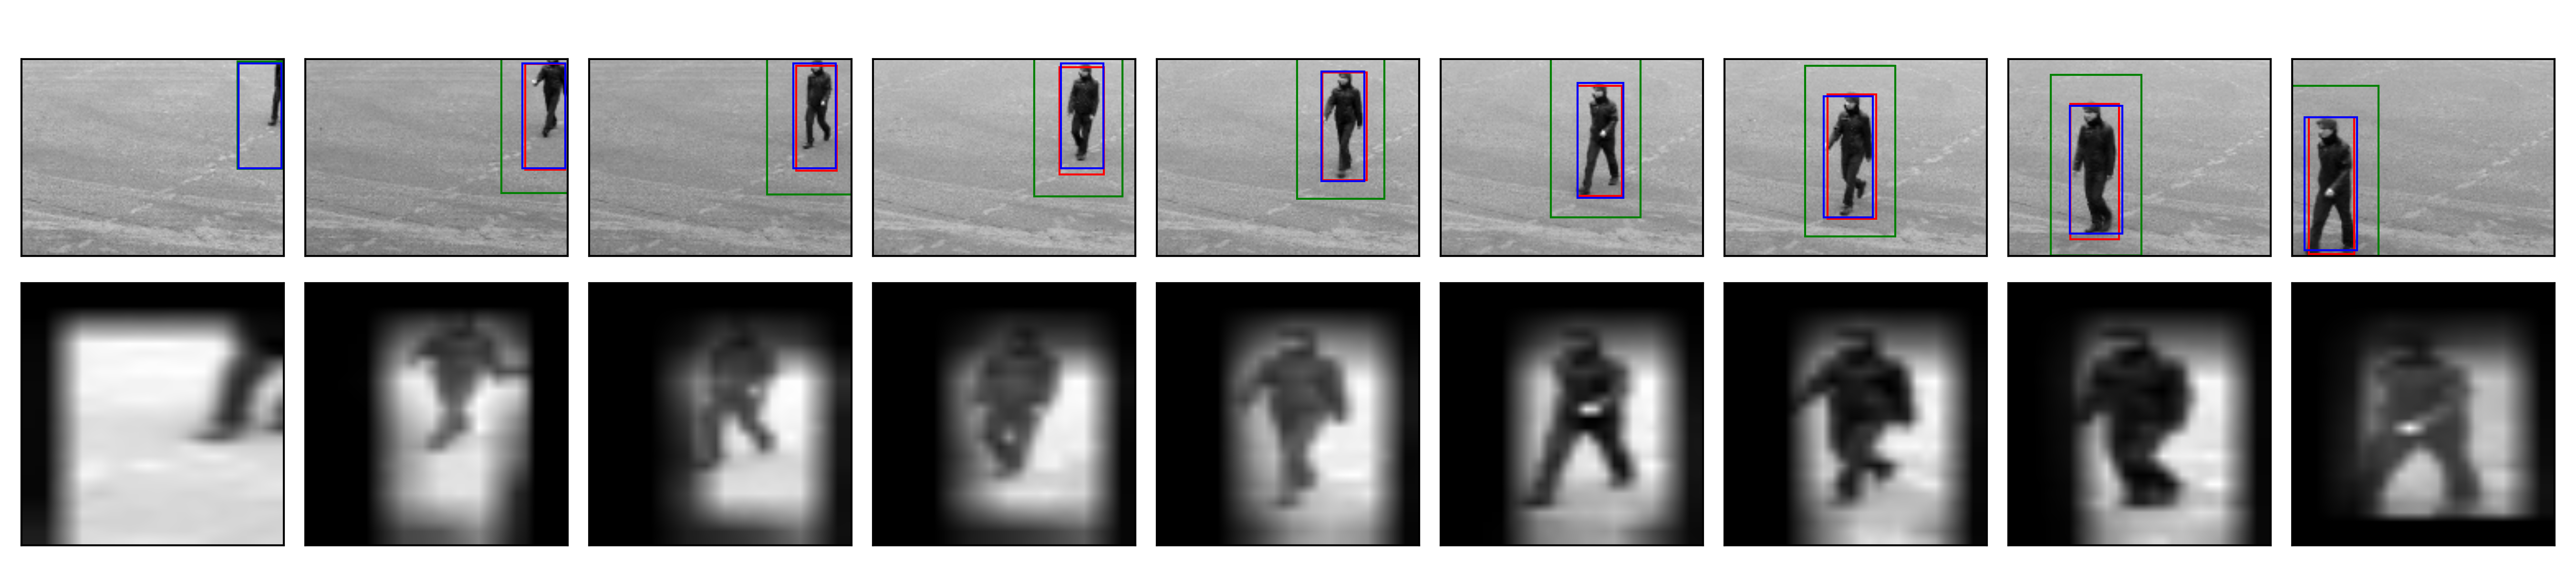
\includegraphics[width=\textwidth]{HART/kth_overlay_16}
		\caption{Tracking results on KTH dataset \cite{KTHActivityRecognition}. Starting with the first initialisation frame where all three boxes overlap exactly, time flows from left to right showing every $16^{th}$ frame of the sequence captured at 25fps. The colour coding follows from  \Cref{fig:img_with_att}. The second row shows attention glimpses multiplied with appearance attention.}
		\label{fig:kth}
	\end{figure}

    \citet{Kahou2015ratm} performed a pedestrian tracking experiment on the KTH activity recognition dataset \cite{KTHActivityRecognition} as a real-world case-study. We replicate this experiment for comparison. We use code provided by the authors for data preparation and we also use their pre-trained feature extractor. Unlike them, we did not need to upscale ground-truth bounding boxes by a factor of 1.5 and then downscale them again for evaluation. We follow the authors and set the glimpse size $\fences{h, w} = \fences{28, 28}$. We replicate the training procedure exactly, with the exception of using the RMSProp optimiser \cite{Tieleman2012rms} with learning rate of $3.33 \times 10^{-5}$ and momentum set to $0.9$ instead of the stochastic gradient descent with momentum. The original work reported an IoU of 55.03\% on average, on test data, while the presented work achieves an average IoU score of 77.11\%, reducing the relative error by almost a factor of two. \Cref{fig:kth} presents qualitative results.
    
  \subsection{Scaling to Real-World Data: KITTI}
	
\begin{figure}
    \RawFloats
    \centering
    \begin{minipage}[c]{0.6\linewidth}
        \centering
	   %
	    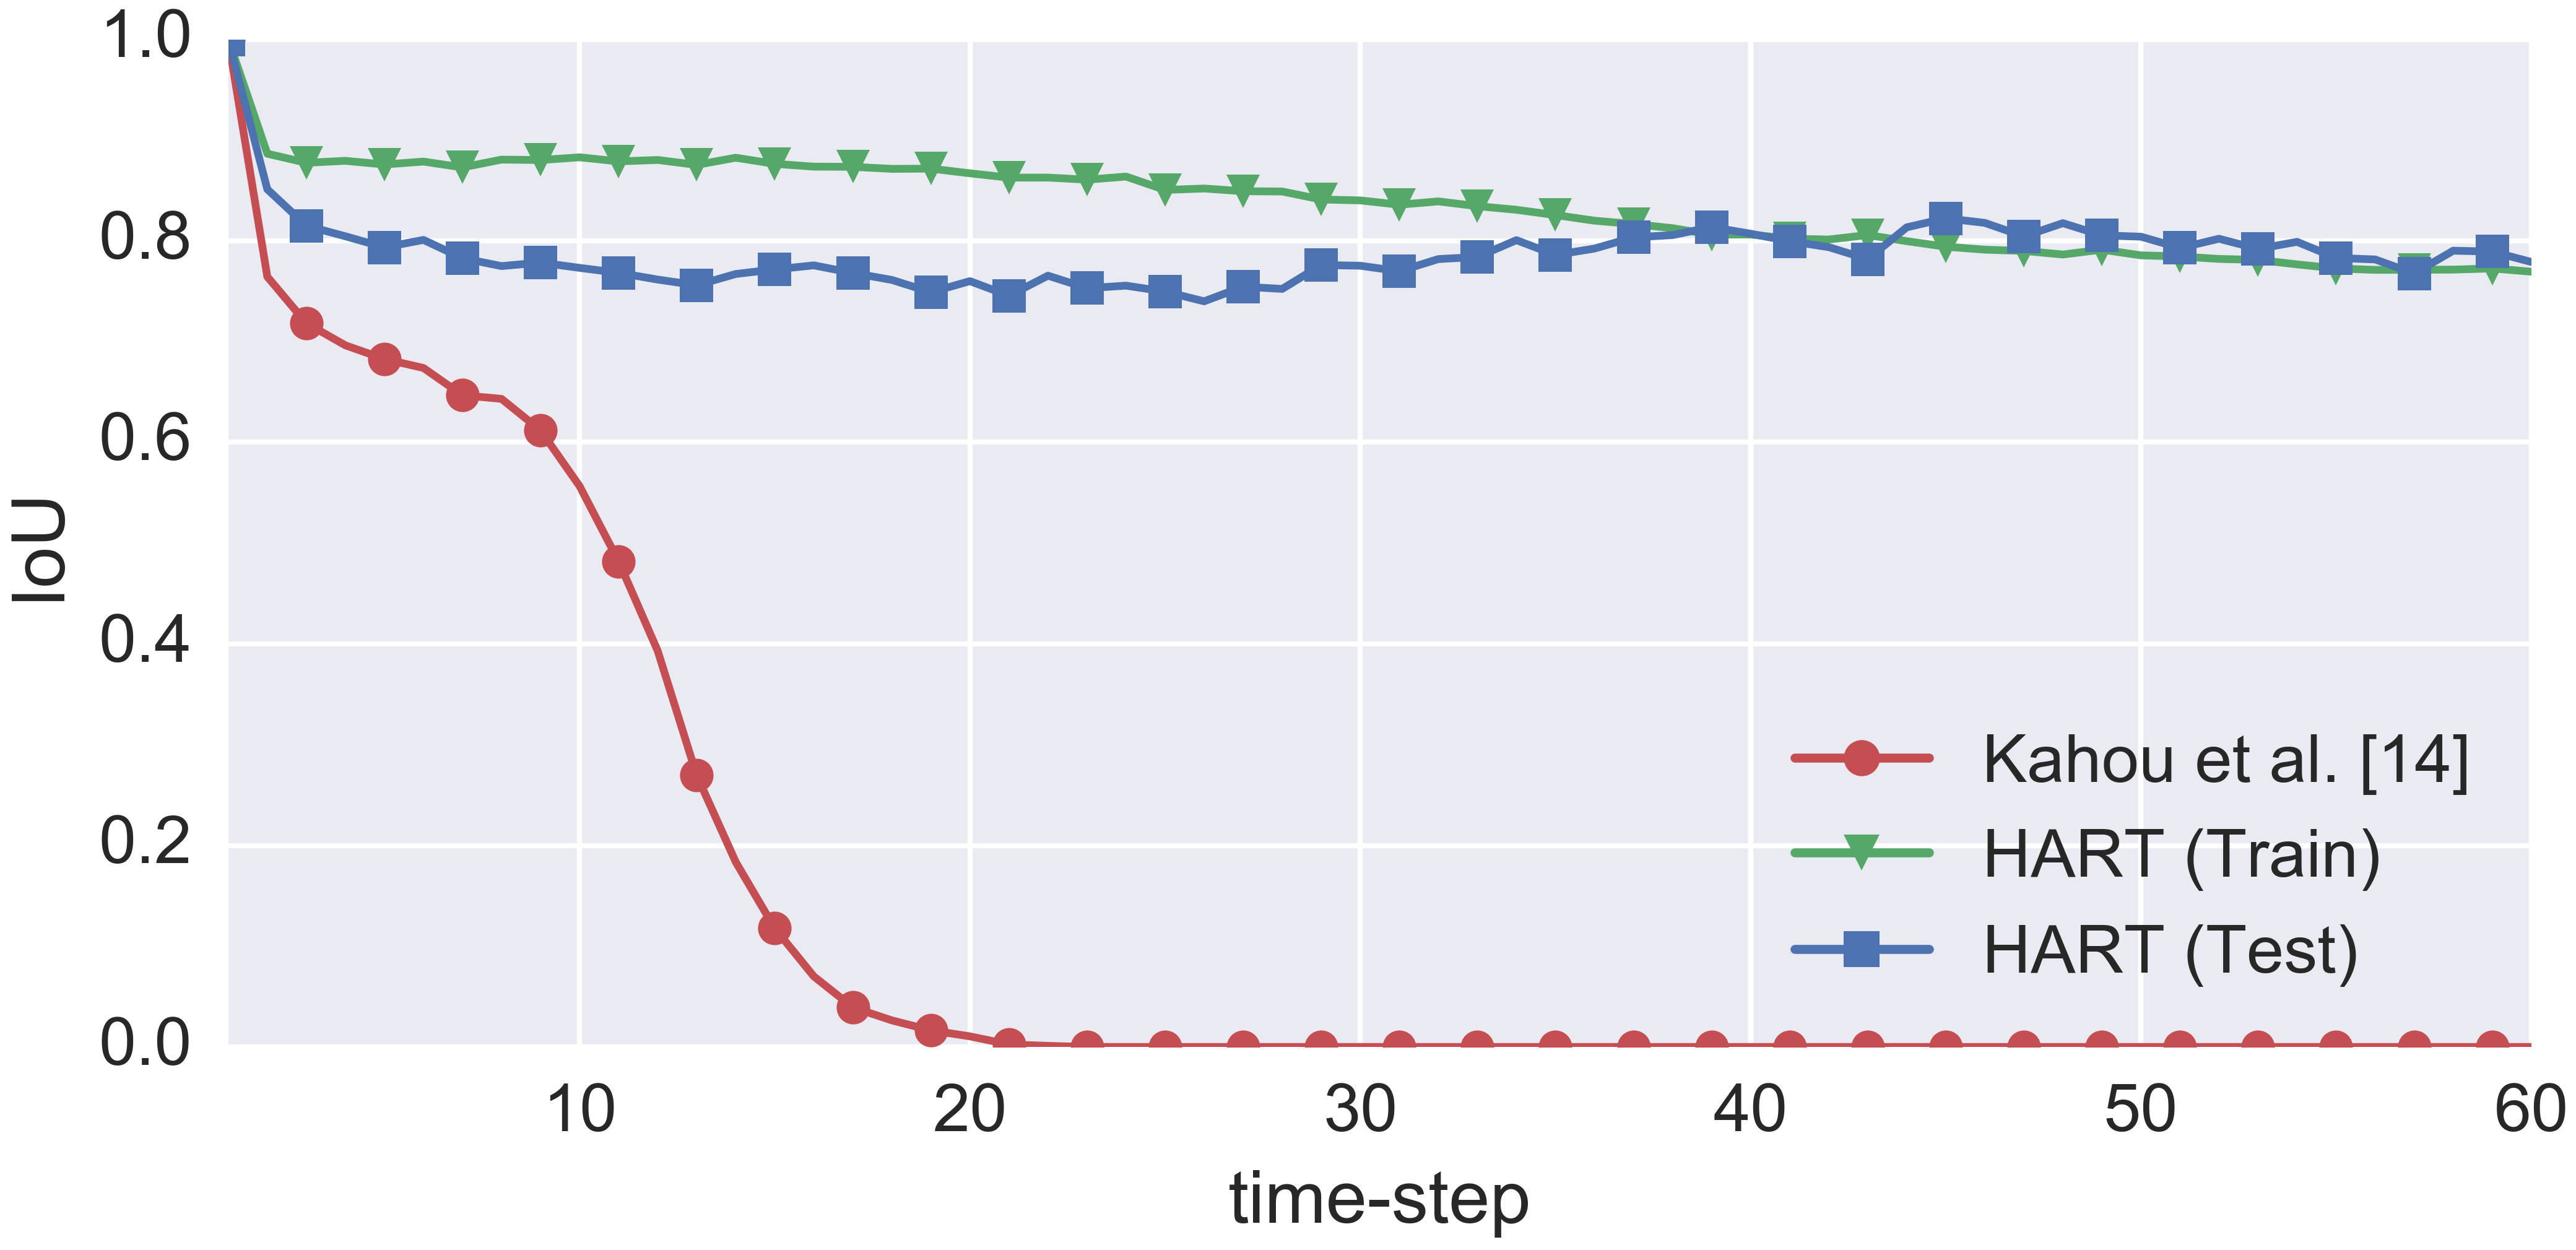
\includegraphics[width=\textwidth]{HART/kitti_iou_fig}
	    \captionof{figure}{IoU curves on KITTI over 60 timesteps. HART (train) presents evaluation on the train set (we do not overfit).}
	    \label{fig:kitti_iou_fig}
    \end{minipage}
    \hfill
    \begin{minipage}[c]{0.35\linewidth}
    	\centering
    	\hspace{-1em}
    	{\small
    	 \begin{tabular}{c|c}
    		\toprule
    		Method                      &   Avg. IoU\\
    		\midrule
    		\citet{Kahou2015ratm}       &   0.14      \\
    		Spatial Att                 &   0.60       \\  
    		App Att                     &   0.78       \\
    		HART                        &   \B{0.81}   \\
    		\bottomrule
    	\end{tabular}
    	}
    	\vspace*{3.3em}
		\captionof{table}{Average IoU on KITTI over 60 time-steps.}
    	\label{tab:kitti}
    \end{minipage}
\end{figure}

    Since we demonstrated that pedestrian tracking is feasible using the proposed architecture, we proceed to evaluate our model in a more challenging multi-class scenario on the KITTI dataset \cite{Geiger2013}. It consists of 21 high resolution video sequences with multiple instances of the same class posing as potential distractors. We split all sequences into 80/20 sequences for train and test sets, respectively. As images in this dataset are much more varied, we implement V1 as the first three convolutional layers of a modified AlexNet \cite{Krizhevsky2012}. The original AlexNet takes inputs of size $227 \times 227$ and downsizes them to $14 \times 14$ after \emph{conv3} layer. Since too low resolution would result in low tracking performance, and we did not want to upsample the extracted glimpse, we decided to replace the initial stride of four with one and to skip one of the max-pooling operations to conserve spatial dimensions. This way, our feature map has the size of $14 \times 14 \times 384$ with the input glimpse of size $\fences{h, w} = \fences{56, 56}$. We apply dropout with probability 0.25 at the end of V1. The ventral stream is comprised of a single convolutional layer with a $1 \times 1$ kernel and five output feature maps. The dorsal stream has two dynamic filter layers with kernels of size $1 \times 1$ and $3 \times 3$, respectively and five feature maps each. We used 100 hidden units in the RNN with orthogonal initialisation and Zoneout \cite{Krueger2016} with probability set to 0.05. The system was trained via curriculum learning \cite{Bengio2009}, by starting with sequences of length five and increasing sequence length every 13 epochs, with epoch length decreasing with increasing sequence length. We used the same optimisation settings, with the exception of the learning rate, which we set to $3.33 \times 10^{-6}$.
    
    
    \Cref{tab:kitti} and \Cref{fig:kitti_iou_fig} contain results of different variants of our model and of the RATM tracker by \citet{Kahou2015ratm} related works. \emph{Spatial Att} does not use appearance attention, nor loss on attention parameters. \emph{App Att} does not apply any loss on appearance attention, while \emph{HART} uses all described modules; it is also our biggest model with 1.8 million parameters. Qualitative results in the form of a video with bounding boxes and attention are available online \footnote{\url{https://youtu.be/Vvkjm0FRGSs}}. We implemented the RATM tracker of \citet{Kahou2015ratm} and trained with the same hyperparameters as our framework, since both are closely related. It failed to learn even with the initial curriculum of five time-steps, as RATM cannot integrate the frame $\bxt$ into the estimate of $\bbt$ (it predicts location at the next time-step). Furthermore, it uses feature-space distance between ground-truth and predicted attention glimpses as the error measure, which is insufficient on a dataset with rich backgrounds. It did better when we initialised its feature extractor with weights of our trained model but, despite passing a few stags of the curriculum, it achieved very poor final performance. 
\section{Discussion}
\label{sec:hart_discussion}
    
    
    % \begin{figure}
    %     \centering
    %     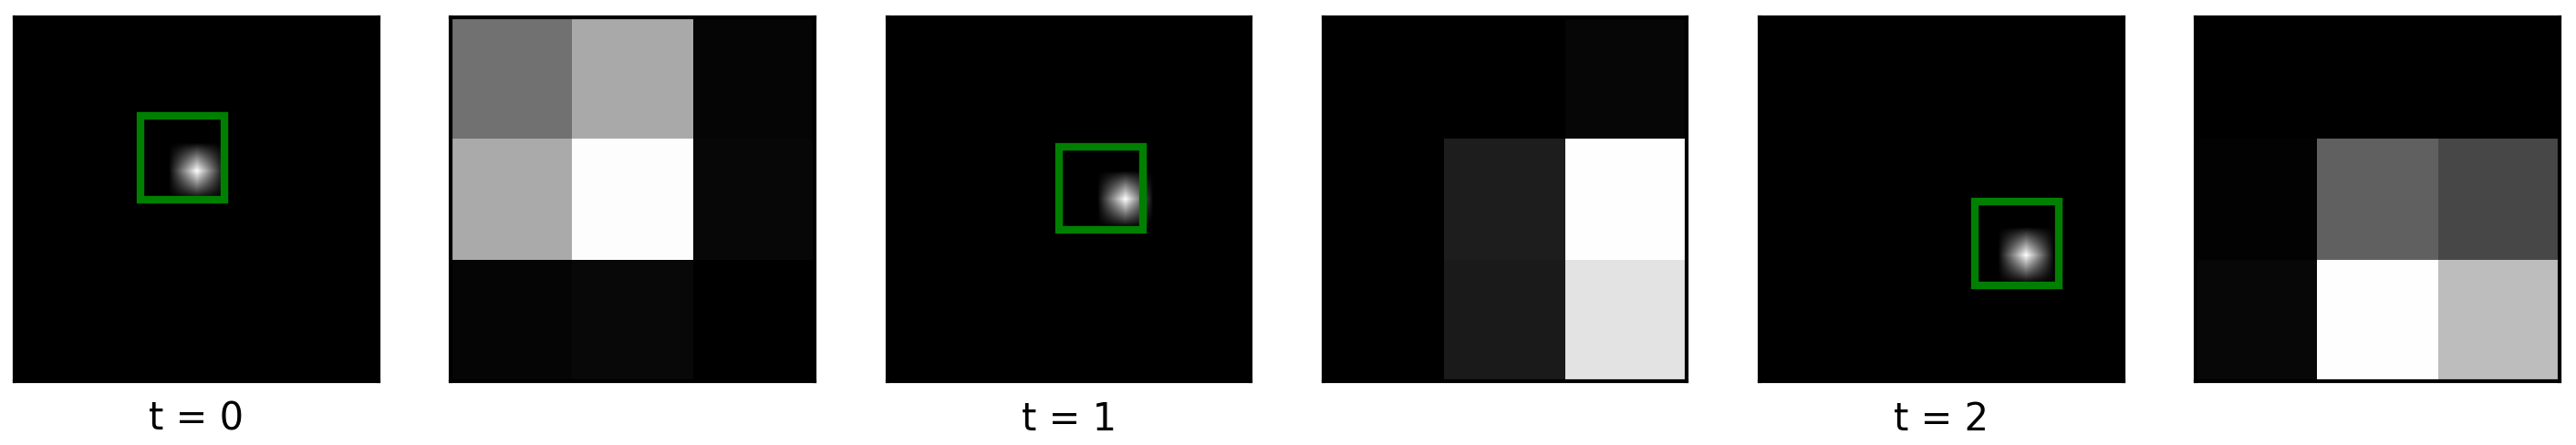
\includegraphics[width=\textwidth]{att_loss_expr}
    %     \caption{Setup for tracking a single white dot on a black background. This simple setup allows to evaluate influence of different loss components on learning.}
    %     \label{fig:att_min_setup}
    % \end{figure}
    
      \begin{figure}
      \centering
      \begin{subfigure}[b]{\textwidth}
        \centering
        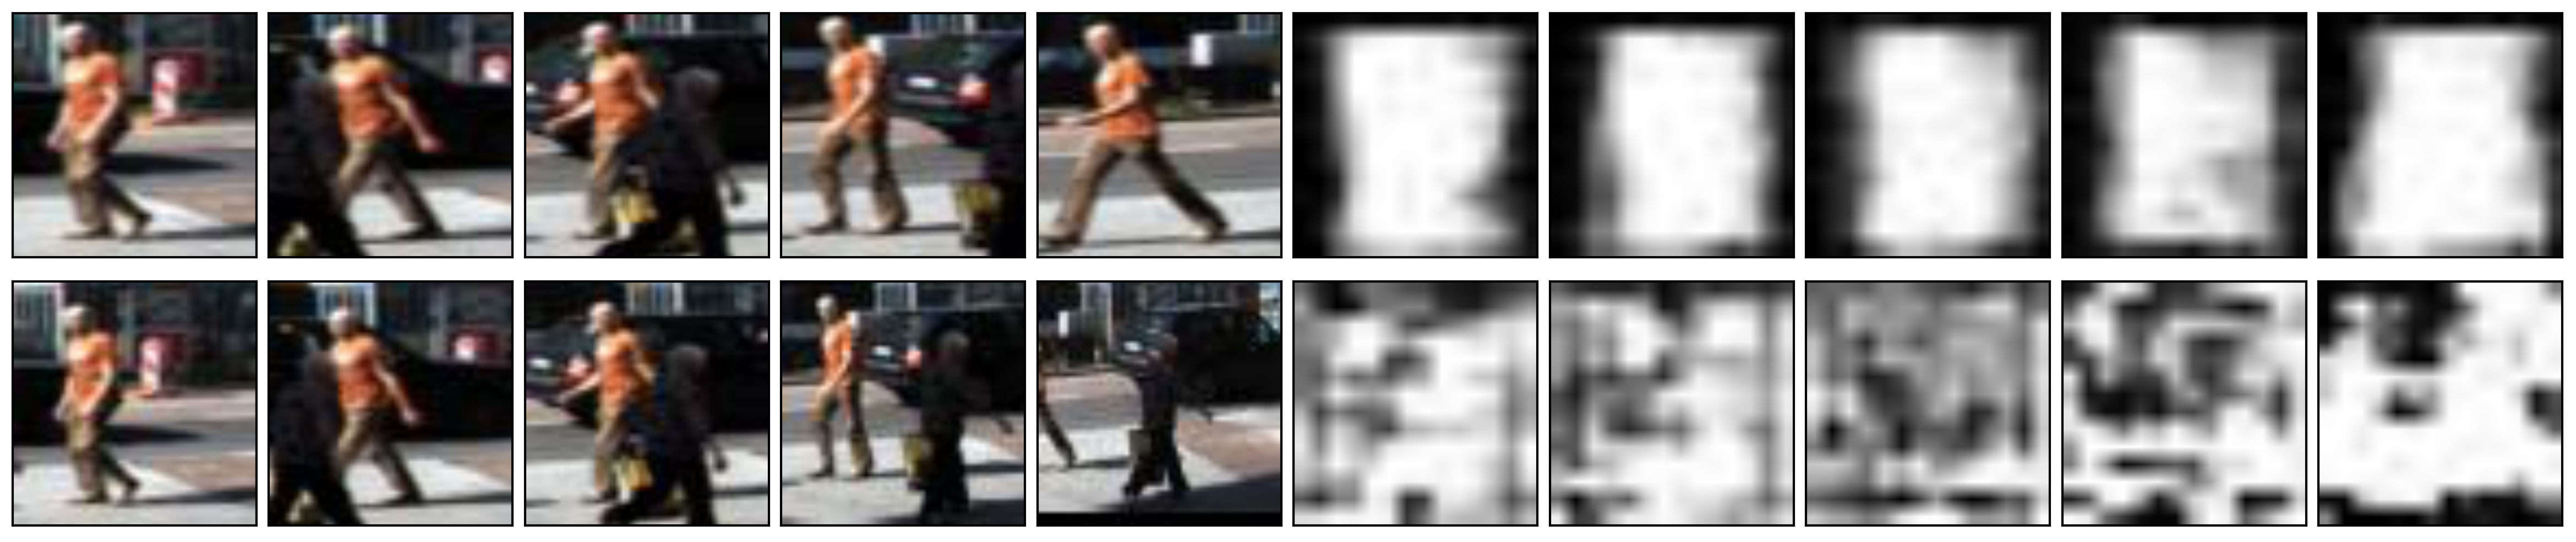
\includegraphics[width=\textwidth]{HART/soft_id_swap}
        \subcaption{The model with appearance attention loss (top) learns to focus on the tracked object, which prevents an ID swap when a pedestrian is occluded by another one (bottom).}
        \label{fig:soft_id_swap}
      \end{subfigure}
      
      \begin{subfigure}[b]{\textwidth}
        \centering
        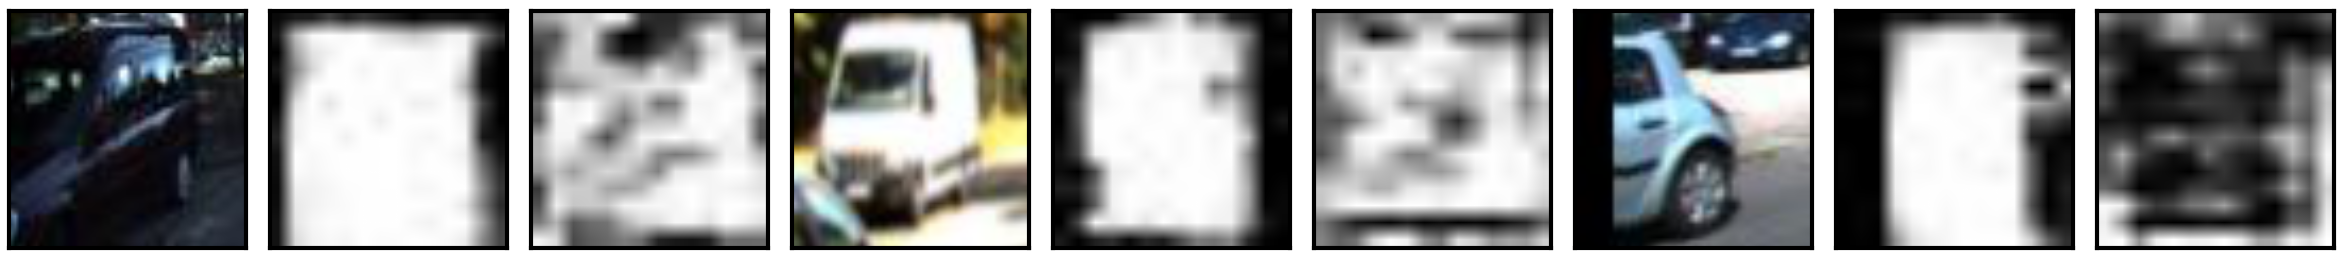
\includegraphics[width=\textwidth]{HART/soft_att}
        \subcaption{Three examples of glimpses and locations maps for a model with and without appearance loss (left to right). Attention loss forces the appearance attention to pick out only the tracked object, thereby suppressing distractors.}
        \label{fig:soft_att_examples}
      \end{subfigure}
      
      \caption{Glimpses and corresponding location maps for models trained with and without appearance loss. The appearance loss encourages the model to learn foreground/background segmentation of the input glimpse.}
      \label{fig:soft_att}
    \end{figure}
    
  
    The experiments in the previous section show that it is possible to track real-world objects with a recurrent attentive tracker. While similar to the tracker by \citet{Kahou2015ratm}, our approach uses additional building blocks, specifically: 
%    \begin{enumerate*}[label=(\roman*)]
	\begin{inparaenum}[(i)]
        \item bounding-box regression loss,
        \item loss on spatial attention,
        \item appearance attention with an additional loss term, and
        \item combines all of these in a unified approach.
%    \end{enumerate*}
	\end{inparaenum}
    We now discuss properties of these modules.
    \begin{description}[leftmargin=\parindent]
        \item[Spatial Attention Loss prevents Vanishing Gradients]        
        Our early experiments suggest that using only the tracking loss causes an instance of the vanishing gradient problem. Early in training, the system is not able to estimate object's motion correctly, leading to cases where the extracted glimpse does not contain the tracked object or contains only a part thereof. In such cases, the supervisory signal is only weakly correlated with the model's input, which prevents learning. Even when the object is contained within the glimpse, the gradient path from the loss function is rather long, since any teaching signal has to pass to the previous timestep through the feature extractor stage. Penalising attention parameters directly seems to solve this issue.
        
        \item[Is Appearance Attention Loss Necessary?]
        Given enough data and sufficiently high model capacity, appearance attention should be able to filter out irrelevant input features before updating the working memory. In general, however, this behaviour can be achieved faster if the model is constrained to do so by using an appropriate loss. \Cref{fig:soft_att} shows examples of glimpses and corresponding location maps for a model with and without loss on the appearance attention. In \cref{fig:soft_id_swap} the model with loss on appearance attention is able to track a pedestrian even after it was occluded by another human. \Cref{fig:soft_att_examples} shows that, when not penalised, location map might not be very object-specific and can miss the object entirely (right-most figure). By using the appearance attention loss, we not only improve results but also make the model more interpretable.
    
        \item[Spatial Attention Bias is Always Positive]
        To condition the system on the object's appearance and make it independent of the starting location, we translate the initial bounding box to attention parameters, to which we add a learnable bias, and create the hidden state of LSTM from corresponding visual features. In our experiments, this bias always converged to positive values favouring attention glimpse slightly larger than the object bounding box. It suggests that, while discarding irrelevant features is desirable for object tracking, the system as a whole learns to trade off attention responsibility between the spatial and appearance based attention modules.
        
        
    \end{description}
\section{Conclusion}
\label{sec:hart_conclusion}
    
    Inspired by the cascaded attention mechanisms found in the human visual cortex, this work presented a neural attentive recurrent tracking architecture suited for the task of object tracking. Beyond the biological inspiration, the proposed approach has a desirable computational cost and increased interpretability due to location maps, which select features essential for tracking. Furthermore, by introducing a set of auxiliary losses we are able to scale to challenging real world data, outperforming predecessor attempts and approaching state-of-the-art performance. Future research will look into extending the proposed approach to multi-object tracking, as unlike many single object tracking, the recurrent nature of the proposed tracker offers the ability to attend each object in turn. 
  
\section*{Acknowledgements}
    
  We would like to thank Oiwi Parker Jones and Martin Engelcke for discussions and valuable insights and Neil Dhir for his help with editing the paper. Additionally, we would like to acknowledge the support of the UK’s Engineering and Physical Sciences Research Council (EPSRC) through the Programme Grant EP/M019918/1 and the Doctoral Training Award (DTA). The donation from Nvidia of the Titan Xp GPU used in this work is also gratefully acknowledged.

%{ %put in braces to make references small
%	\balance
%	\small
%% 	\bibliographystyle{unsrt}
%    \bibliographystyle{plainnat}
%	\bibliography{library}
%}

%\appendix
% \input{adaptive_loss}
% \input{questions}

%\end{document}


\chapter{End-to-end Recurrent Multi-Object Tracking and Trajectory Prediction with Relational Reasoning}
\label{ch:mohart}

\begin{abstract}
	The majority of contemporary object-tracking approaches used in autonomous vehicles do not model interactions between objects. This contrasts with the fact that objects' paths are not independent: a cyclist might abruptly deviate from a previously planned trajectory in order to avoid colliding with a car.
	Building upon \textsc{hart}, a neural, class-agnostic single-object tracker, we introduce a multi-object tracking method (\textsc{mohart}) capable of \emph{relational reasoning}. Importantly, the entire system, including the understanding of interactions and relations between objects, is class-agnostic and learned simultaneously in an end-to-end fashion.
	We find that the addition of relational-reasoning capabilities to \textsc{hart} leads to consistent performance gains in tracking as well as future trajectory prediction on several real-world datasets (MOTChallenge, UA-DETRAC, and Stanford Drone dataset), particularly in the presence of ego-motion, occlusions, crowded scenes, and faulty sensor inputs.
	Finally, based on controlled simulations, we propose that a comparison of \textsc{mohart} and \textsc{hart} may be used as a novel way to measure the degree to which the objects in a video depend upon each other as they move together through time. 
\end{abstract}

%===============================================================================

\section{Introduction}
\label{sec:mohart_intro}


\begin{figure}[b!]
    \centering
    \begin{subfigure}[c]{0.41\linewidth}
        \centering
        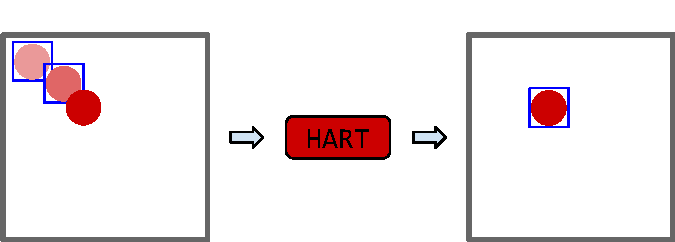
\includegraphics[width=\linewidth]{figures/MOHART/system_hart}
        \caption{HART}
    \end{subfigure}
    \hspace{20mm}
    \begin{subfigure}[c]{0.41\linewidth}
        \centering
        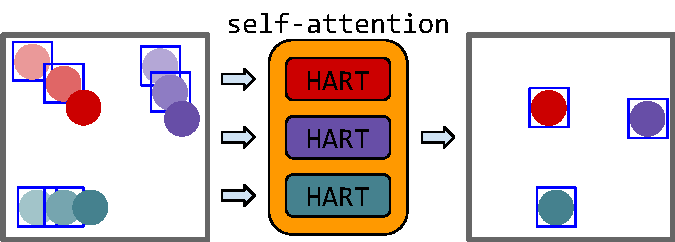
\includegraphics[width=\linewidth]{figures/MOHART/system_mohart}
        \caption{MOHART}
    \end{subfigure}
    \caption{
    Single-object tracking with \gls{HART} (left) and our extension to multi-object tracking (\gls{MOHART}, right). In our proposed framework, the different \gls{HART} trackers are connected via a relational reasoning module allowing for more robust tracking and more accurate future trajectory prediction.
    % \vspace{-4mm}
    }
    \label{fig:teaser}
\end{figure}

Autonomous vehicles need to operate in rich environments that contain a large variety of interacting object. 
%
This variety motivates the need for \emph{class-agnostic} object trackers, which break with the popular tracking-by-detection paradigm \cite{Zhang2008,Milan2014,Bae2017confidence, Keuper2018motion}. 
%
In tracking-by-detection, static video frames are first analysed by an object detector,\eg a pre-trained deep \gls{CNN} such as \textsc{yolo} \citep{Redmon15}, and then the detected objects are linked across frames. 
%
Algorithms from this family can achieve high accuracy, provided sufficient labelled data to train the object detector, and given that all encountered objects can be associated with known classes. 
%

\Gls{HART} is a recently proposed alternative for single-object tracking (\textsc{sot}), where an arbitrary object can be tracked from an initial video frame \citep{Kosiorek2017hierch}.
%
Since the initial bounding-box is user-provided and may be placed over any part of the image, regardless of whether it corresponds to an object and its class, \gls{HART} can track arbitrary objects.
% 
\Gls{HART} efficiently processes just the relevant part of an image using spatial attention; it also integrates object detection, feature extraction, and motion modelling into one network, which is trained fully end-to-end.
Contrary to tracking-by-detection, where only one video frame is typically processed at any given time to generate bounding box proposals, end-to-end learning in \gls{HART} allows discovering complex visual and spatio-temporal patterns in videos, which is conducive to inferring what an object is and how it moves.
%

In the original formulation, \gls{HART} is limited to the single-object modality---as are other existing end-to-end trackers \cite{Kahou2015ratm,Danesh2019deep,Gordon2018re3}.
%
In this work, we present \gls{MOHART}, a class-agnostic tracker with complex relational reasoning capabilities provided by a multi-headed self-attention module \citep{Vaswani17,Lee2019set}. 
\Gls{MOHART} infers the latent state of every tracked object in parallel, and uses self-attention to inform per-object states about other tracked objects.
This helps to avoid performance loss under self-occlusions of tracked objects or strong ego-motion.
Moreover, since the model is trained end-to-end, it is able to learn how to manage faulty or missing sensor inputs.
It can also use the inferred objects' states to predict their future trajectories, which depend on interactions between different objects. See \cref{fig:teaser} for a high-level illustration of \gls{HART} and \gls{MOHART}.

After describing related work in \Cref{sec:mohart_related} and the methodology in \cref{sec:mohart_method}, we employ the algorithm on toy domains to validate its efficacy in \Cref{sec:mohart_experiment_toy}. By controlling the stochasticity of toy environments, we show that single-object tracking is sufficient in some cases, even those featuring strong long-range interactions, while it may fail in other cases.
This may hint at a similar phenomenon in the real world: tracking objects or predicting their future motion independently may be possible in most (but not all) cases, while solving the remaining corner cases might require taking interactions between objects into account.
It is these corner cases that motivate our work.
In \Cref{sec:experiment_real}, we test \gls{MOHART} on three real world datasets (MOTChallenge \cite{Mot16}, UA-DETRAC \cite{Wen15}, Stanford Drone dataset \cite{Dronedataset}) and show that relational reasoning between objects is most important on the MOTChallenge dataset. We hypothesise that this is due to its richness in ego-motion, occlusions and crowded scenes---a result supported by our ablation study. Furthermore, we show that \gls{MOHART} is able to gracefully handle missing sensory inputs---without any architectural changes. In this case, it falls back on its internal motion model, which also allows for accurate prediction of object locations multiple time steps into the future, learned in a data-driven manner.




\section{Related Work}\label{sec:related}

\paragraph{Tracking-by-Detection} Vision-based tracking approaches typically follow a tracking-by-detection paradigm: objects are first detected in each frame independently, and then a tracking algorithm links the detections from different frames to propose a coherent trajectory \cite{Zhang2008,Milan2014,bae2017confidence,keuper2018motion}.
Motion models and appearance are often used to improve the association between detected bounding-boxes and multiple trackers in a postprocessing step.
Recently, elements of this pipeline have been replaced with learning-based approaches such as deep learning \cite{Nam2016,Ning2017,keuper2018motion,bae2017confidence} or reinforcement learning \cite{Xiang2015}. Some approaches are targeted towards robustness across domains, for example by using a category-agnostic object detector and performing classification only in a post-processing step \cite{Osep2017,Posner2016}.


 \paragraph{End-to-End Tracking} A newly established and much less explored stream of work approaches tracking in an end-to-end fashion. A key difficulty here is that extracting an image crop (according to bounding-boxes provided by a detector), is non-differentiable and results in high-variance gradient estimators.
 \citet{Kahou15} propose an end-to-end tracker with soft spatial-attention using a 2D grid of Gaussians instead of a hard bounding-box. \Gls{HART} draws inspiration from this idea, employs an additional attention mechanism, and shows promising performance on the real-world KITTI dataset \cite{Kosiorek17}.
 \Gls{HART}, which forms the foundation of this work, is explained in detail in \Cref{sec:method}. It has also been extended to incorporate depth information from \textsc{rgbd} cameras \cite{Danesh19}. \citet{Gordon2018} propose an approach in which the crop corresponds to the scaled up previous bounding-box. This simplifies the approach, but does not allow the model to learn where to look---\ie no gradient is backpropagated through crop coordinates.
 To the best of our knowledge, there are no successful implementations of any such end-to-end approaches for multi-object tracking beyond \textsc{sqair} \citep{Kosiorek2018sqair}, which works only on datasets with static backgrounds. On real-world data, the only end-to-end approaches correspond to applying multiple single-object trackers in parallel---a method which does not leverage the potential of scene context or inter-object interactions. 

\paragraph{Pedestrian trajectory prediction} 
Predicting pedestrian trajectories has a long history in computer vision and robotics.
Initial research modelled social forces using hand-crafted features~\cite{UCY,ETH,IGP,yamaguchi2011you} or \textsc{mdp}-based motion transition models~\cite{rudenko2018joint}, while more recent approaches learn from context information,\eg positions of other pedestrians or landmarks in the environment. Social-\textsc{lstm} \cite{social-lstm} employs a \gls{LSTM} to predict pedestrian trajectories and uses max-pooling to model global social context.
Attention mechanisms have been employed to query the most relevant information, such as neighbouring pedestrians, in a learnable fashion  \cite{su2016crowd, fernando2018soft, sadeghian2019sophie}. 
Apart from relational learning, context \cite{varshneya2017human}, periodical time information \cite{sun20183dof}, and constant motion priors \cite{scholler2019simpler} have proven effective in predicting long-term trajectories. 

Our work stands apart from this prior art by not relying on ground truth tracklets. Instead, it addresses the more challenging task of working directly with visual input, performing tracking, modelling interactions, and, depending on the application scenario, simultaneously predicting future motions. As such, it can also be compared to Visual Interaction Networks (\textsc{vin}) \cite{Watters2017}, which use a \gls{CNN} to encode three consecutive frames into state vectors---one per object---and feeds these into a \gls{RNN}, which has an Interaction Network \cite{Battaglia2016} at its core. 
% added sentence
More recently, Relational Neural Expectation Maximization (\textsc{r-nem}) has been proposed as an unsupervised approach which combines scene segmentation and relational reasoning \cite{Steenkiste2018}.
Both \textsc{Vin}s and \textsc{r-nem} are able to make accurate predictions in physical scenarios, but, to the best of our knowledge, have not been applied to real world data.

\section{Recurrent Multi-Object Tracking with Self-Attention}
%\vspace{-3mm}
\label{sec:mohart_method}

\begin{figure}
	\centering
	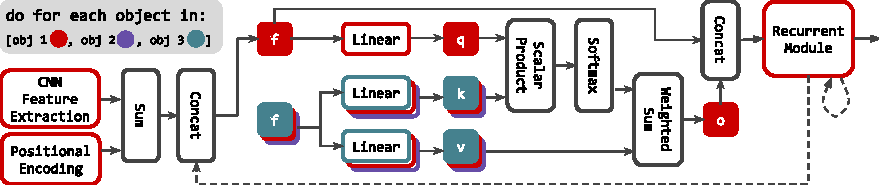
\includegraphics[width=\linewidth]{figures/MOHART/sab.pdf}
	\caption{
		The relational reasoning module in \Gls{MOHART} based on multi-headed self-attention. Here, we show the computation of the interaction of the red object with all other objects. Object representations $f_{t,m}$ are computed using visual features, positional encoding and the hidden state from the recurrent module. These are linearly projected onto keys (k), queries (q), and values (v) to compute a weighted sum of interactions between objects, yielding an interaction vector $o_{t,m}$. Subscripts $t, m$ are dropped from all variables for clarity of presentation, so is the splitting into multiple heads.
	}
	\label{fig:sab}
\end{figure}

This section describes the model architecture in \cref{fig:teaser}. We start by describing the \glsreset{HART}\gls{HART} algorithm of \Cref{ch:hart}, and then follow with an extension of \gls{HART} to tracking multiple objects, where multiple instances of \gls{HART} communicate with each other using multi-headed attention to facilitate relational reasoning. We also explain how this method can be extended to trajectory prediction instead of just tracking. 

\subsection{Hierarchical Attentive Recurrent Tracking (\textsc{hart})}
\vspace{-3mm}
%\vspace{-.5em}
%\paragraph{Hierarchical Attentive Recurrent Tracking (\textsc{hart})}
\textsc{Hart} is an attention-based recurrent algorithm, which can efficiently track single objects in a video.
It uses a spatial attention mechanism to extract a \textit{glimpse} $\bg_t$, which corresponds to a small crop of the image $\bxt$ at time-step $t$, containing the object of interest.
This allows it to dispense with the processing of the whole image and can significantly decrease the amount of computation required.
\Gls{HART} uses a \gls{CNN} to convert the glimpse $\bg_t$ into features $\mathbf{f}_t$, which then update the hidden state $\mathbf{h}_t$ of a \gls{LSTM} core.
The hidden state is used to estimate the current bounding-box $\mathbf{b}_t$, spatial attention parameters for the next time-step $\ba_{t+1}$, as well as object appearance.
Importantly, the recurrent core can learn to predict complicated motion conditioned on the past history of the tracked object, which leads to relatively small attention glimpses---contrary to \gls{CNN}-based approaches \citep{Held2016goturn,Valmadre2017}, \gls{HART} does not need to analyse large regions-of-interest to search for tracked objects.
In the original paper, \textsc{hart} processes the glimpse with an additional ventral and dorsal stream on top of the feature extractor. Early experiments have shown that this does not improve performance on the MOTChallenge dataset, presumably due to the oftentimes small objects and overall small amount of training data. 
Further details are provided in \Cref{sec:mohart_architecture_details}.

	The algorithm is initialised with a bounding-box\footnote{We can use either a ground-truth bounding-box or one provided by an external detector; the only requirement is that it contains the object of interest.} $\mathbf{b}_1$ for the first time-step, and operates on a sequence of raw images $\bx_{1:T}$.
	For time-steps $t\geq2$, it recursively outputs bounding-box estimates for the current time-step and predicted attention parameters for the next time-step. The performance is measured as intersection-over-union (IoU) averaged over all time steps in which an object is present, excluding the first time step.

Although \gls{HART} can track arbitrary objects, it is limited to tracking one object at a time.
While it can  be deployed on several objects in parallel, different \gls{HART} instances have no means of communication.
This results in performance loss, as it is more difficult to identify 
occlusions, ego-motion and object interactions.
Below, we propose an extension of \gls{HART} which remedies these shortcomings.

\subsection{Multi-Object Hierarchical Attentive Recurrent Tracking (\textsc{mohart})}
\vspace{-3mm}
%\vspace{-.5em}
%\paragraph{Multi-Object Hierarchical Attentive Recurrent Tracking (\textsc{mohart})}
Multi-object support in \gls{HART} requires the following modifications.
Firstly, in order to handle a dynamically changing number of objects, we apply \gls{HART} to multiple objects in parallel, where all parameters between \gls{HART} instances are shared. 
We refer to each \gls{HART} instance as a \textit{tracker}.
Secondly, we introduce a presence variable $p_{t,m}$ for object $m$.
It is used to mark whether an object should interact with other objects, as well as to mask the loss function (described in \Cref{ch:hart}) for the given object when it is not present.
In this setup, parallel trackers cannot exchange information and are conceptually still single-object trackers, which we use as a baseline, referred to as \gls{HART} (despite it being an extension of the original algorithm).
Finally, to enable communication between trackers, we augment \gls{HART} with an additional step between feature extraction and the \gls{LSTM}.

For each object, a glimpse is extracted and processed by a CNN (see \cref{fig:teaser}). Furthermore, spatial attention parameters are linearly projected on a vector of the same size and added to this representation, acting as a positional encoding. This is then concatenated with the hidden state of the recurrent module of the respective object (see \cref{fig:sab}). Let $\mathbf{f}_{t, m}$ denote the resulting feature vector corresponding to the m$^\mathrm{th}$ object, and let $\mathbf{f}_{t, 1:M}$ be the set of such features for all objects.
Since different objects can interact with each other, it is necessary to use a method that can inform each object about the effects of their interactions with other objects.
Moreover, since features extracted from different objects comprise a set, this method should be permutation-equivariant,\ie the results should not depend on the order in which object features are processed.
Therefore, we use the multi-head self-attention block (\textsc{sab}, \citet{Lee2019set}), which is able to account for higher-order interactions between set elements when computing their representations. %, thereby allowing rich information exchange, and it can do so in a permutation-equivariant manner.
Intuitively, in our case, \textsc{sab} allows any of the trackers to query other trackers about attributes of their respective objects,\eg distance between objects, their direction of movement, or their relation to the camera.
This is implemented as follows,
\begin{align}
Q &= W_q \mathbf{f}_{1:M} + b_q\,, \qquad K = W_k \mathbf{f}_{1:M} + b_k\,, \qquad V = W_v \mathbf{f}_{1:M} + b_v \label{eq:projection}\,,\\
&\hspace{1.5em} O_i = \operatorname{softmax}\left( Q_i K_i^T \right) V_i\,, \qquad i=1,\dots,H\,, \label{eq:att}\\
&\hspace{7em} o_{1:M} = O = \operatorname{concat}(O_i,\dots,O_H)\,, \label{eq:multihead}
\end{align}
where $o_m$ is the output of the relational reasoning module for object $m$. Time-step subscripts are dropped to decrease clutter.
In Eq. \ref{eq:projection}, each of the extracted features $\mathbf{f}_{t,m}$ is linearly projected into a triplet of key $\mathbf{k}_{t,m}$, query $\mathbf{q}_{t,m}$ and value $\mathbf{v}_{t,m}$ vectors. Together, they comprise $K, Q$ and $V$ matrices with $M$ rows and $d_q, d_k, d_k$ columns, respectively.
$K, Q$ and $V$ are then split up into multiple heads $H \in \mathbb{N}_+$, which allows to query different attributes by comparing and aggregating different projection of features.
Multiplying $Q_iK_i^T$ in Eq. \ref{eq:att} allows to compare every query vector $\mathbf{q}_{t,m,i}$ to all key vectors $\mathbf{k}_{t,1:M,i}$, where the value of the corresponding dot-products represents the degree of similarity.
Similarities are then normalised via a $\operatorname{softmax}$ operation and used to aggregate values $V$.
Finally, outputs of different attention heads are concatenated in Eq. \ref{eq:multihead}.
\textsc{Sab} produces $M$ output vectors, one for each input, which are then concatenated with corresponding inputs and fed into separate \gls{LSTM}s for further processing, as in \gls{HART}---see \cref{fig:teaser}.


\begin{figure}[t!]%
	\centering
	\includegraphics[width=0.99\textwidth]{figures/MOHART/mot_proel.pdf}
	% \vspace{-3mm}
	\caption{
		A scenario constructed to be impossible to solve without relational reasoning. Circles of the same colour repel each other, circles of different colour attract each other. Crucially, each circle is randomly assigned its identity in each time step. Hence, the algorithm can not infer the forces exerted on one object without knowledge of the state of the other objects in the current time step. The forces in this scenario scale with $1/\sqrt{r}$ and the algorithm was trained to predict one time step into the future. \textsc{hart} (top) is indeed unable to predict the future location of the objects accurately. The achieved average IoU is $47\%$, which is only slightly higher than predicting the objects to have the same position in the next time step as in the current one ($34\%$). Using the relational reasoning module, \textsc{mohart} (bottom) is able to make meaningful predictions ($76\%$ IoU). The numbers in the bottom row indicate the self-attention weights from the perspective of the top left tracker (yellow number box). Interestingly, the attention scores have a strong correlation with the interaction strength (which scales with distance) without receiving supervision.
		\vspace{-3mm}
	}
	\label{fig:toy2}
\end{figure}


\Gls{MOHART} is trained fully end-to-end, contrary to other tracking approaches. % \citep{Zhang2008,Milan2014,bae2017confidence,keuper2018motion}.
It maintains a hidden state, which can contain information about the object's motion. One benefit is that in order to predict future trajectories, one can simply feed black frames into the model. Our experiments show that the model learns to fall back on the motion model captured by the \gls{LSTM} in this case. 


\subsection{Multi-Object Baselines}

\vspace{-.5em}
\paragraph{\Gls{MLP}} In this version, the representations of all objects are concatenated and fed into a fully connected layer followed by ELU activations. The output is then again concatenated to the unaltered feature vector of each object. This concatenated version is then fed to the recurrent module of \gls{HART}. This way of exchanging information allows for universal function approximation (in the limit of infinite layer sizes) but does not impose permutation invariance.


\vspace{-.5em}
\paragraph{DeepSets} Here, the learned representations of the different objects are summed up instead of concatenated and then divided by total number of objects. 
% This has lower capacity than the \gls{MLP} version. 
This is closely related to DeepSets \citep{Zaheer2017} and allows for universal function approximation of all permutation invariant functions \citep{Wagstaff2019}.

\vspace{-.5em}
\paragraph{Max-Pooling} Similar to DeepSets, but using max-pooling as the permutation invariant operation. This way of exchanging information is used, e.g., by \citet{Alahi2016social} who predict future pedestrian trajectories from ground truth tracklets in coordinate space.



\section{Validation on Simulated Data} %Toy Example
\label{sec:experiment_toy}

\begin{figure}%
    \centering
    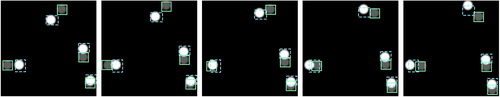
\includegraphics[width=0.99\textwidth]{Figures/sot_protons.png}
    \vspace{-3mm}
    \caption{\textsc{hart} single object tracking applied four times in parallel. Dashed lines indicate spatial attention, solid lines are predicted bounding boxes at time step $T+3$, faded circles show the ground truth location at $T+3$. The repulsive force between each object pair scales with distance as $1/r$. There is no information exchange between the trackers and each tracker evidently only `attends' to its own object. The fact that the future location is predicted accurately (i.e., much better than linear extrapolation) indicates that \textsc{hart} is able to capture complex motion patterns essentially allowing to draw conclusions about the force field. Shown are consecutive time steps from left to right.
    }
    \label{fig:toy1}
\end{figure} 
\begin{figure}%
    \centering
    \includegraphics[width=0.99\textwidth]{Figures/mot_proel.pdf}
    \vspace{-3mm}
    \caption{\textsc{hart} (top, $46\%$ IoU) vs. \textsc{mohart} (bottom, $76\%$ IoU). Dashed lines show spatial attention, solid lines show predicted bounding boxes, faded circles indicate future ground truth locations. Circles of the same colour repel each other, circles of different colours attract each other. The colour coded identities are randomly assigned in each time step rendering information exchange between trackers (i.e. relational reasoning) necessary. The numbers in the bottom row indicate the self-attention weights from the perspective of the top left tracker (yellow number box).
    \vspace{-3mm}
    }
    \label{fig:toy2}
\end{figure}


To test the efficacy of the proposed algorithm, we conduct experiments on a toy domain. First, we show that \textsc{hart} as an end-to-end single-object tracker is able to capture complex motion patterns and leverage these to make accurate predictions. Second, we create a scenario which is not solvable for a single object tracker as it requires knowledge about the state of the other objects and relational reasoning. We show that \textsc{mohart}, using self-attention for relational reasoning, is able to capture these interactions with high accuracy and compare it to other possible implementations of \textsc{mohart} (e.g., using max-pooling instead of self-attention). In order to accurately investigate the model's understanding of motion patterns and interactions between objects, in contrast to traditional tracking, the model is not trained to predict the current location of the object, but its location in a future time step. The domain we create for this purpose is a two dimensional squared box. It contains circular objects with approximated elastic collisions (energy and momentum conservation) between objects and with walls (see \Cref{fig:toy1,fig:toy2}).

In the first scenario (\Cref{fig:toy1}), four circles each exert repulsive forces on each other, where the force scales with $1/r$, $r$ being their distance. \textsc{hart} is applied four times in parallel and is trained to predict the location of each circle three time steps into the future. The different forces from different objects lead to a non-trivial force field at each time step. Predicting the future location just using the previous motion of one object (\Cref{fig:toy1} shows that each spatial attention box covers only the current object) accurately is therefore challenging. Surprisingly, the single object tracker solves this task with an average of $95\%$ IoU over sequences of 15 time steps. This shows the efficacy of end-to-end tracking to capture complex motion patterns and use them to predict future locations. This, of course, could also be used to generate robust bounding boxes for a tracking task.

The second scenario (\Cref{fig:toy2}) is constructed to be impossible to solve without exchanging information between objects. This is achieved by introducing two colour-coded identities. Agents of the same identity repel each other, agents of different identities attract each other. Crucially, each agent is randomly assigned its identity in each time step. Hence, the algorithm can no longer infer the forces exerted on one object without knowledge of the state of the other objects in the current time step. The forces in this scenario scale with $1/\sqrt{r}$ and the algorithm was trained to predict one time step into the future. \textsc{hart} is indeed unable to predict the future location of the objects accurately (\Cref{fig:toy2} - top). The achieved average IoU is $47\%$, which is only slightly higher than predicting the objects to have the same position in the next time step as in the current one ($34\%$). A possible interpretation of the qualitative results (green boxes in \Cref{fig:toy2} - top) is that the model uses the momentum of each object to extrapolate into the future. This sometimes works well (bottom right object in frame 31) and sometimes not (top right object in frame 30). Using the relational reasoning module (\Cref{fig:toy2} - bottom), the model is now able to make meaningful predictions ($76\%$ IoU). Interestingly, in each frame, the attention scores have a strong correlation with the interaction strength (which directly scales with distance). Despite this not being necessary for the relational reasoning module, this is an interesting side-product as it did not receive any direct supervision.

\begin{figure}
    \centering
    \begin{subfigure}[c]{0.49\linewidth}
        \centering
        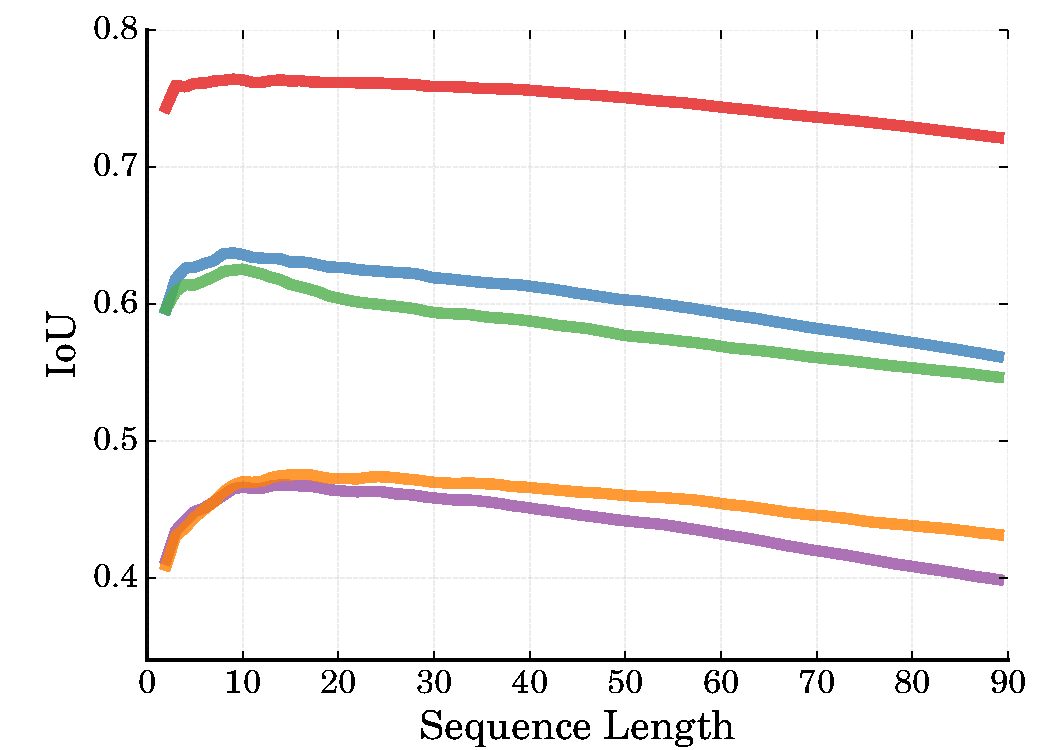
\includegraphics[width=\linewidth]{Figures/toy_iou_over_timesteps.pdf}
    \end{subfigure}
    \begin{subfigure}[c]{0.49\linewidth}
        \centering
        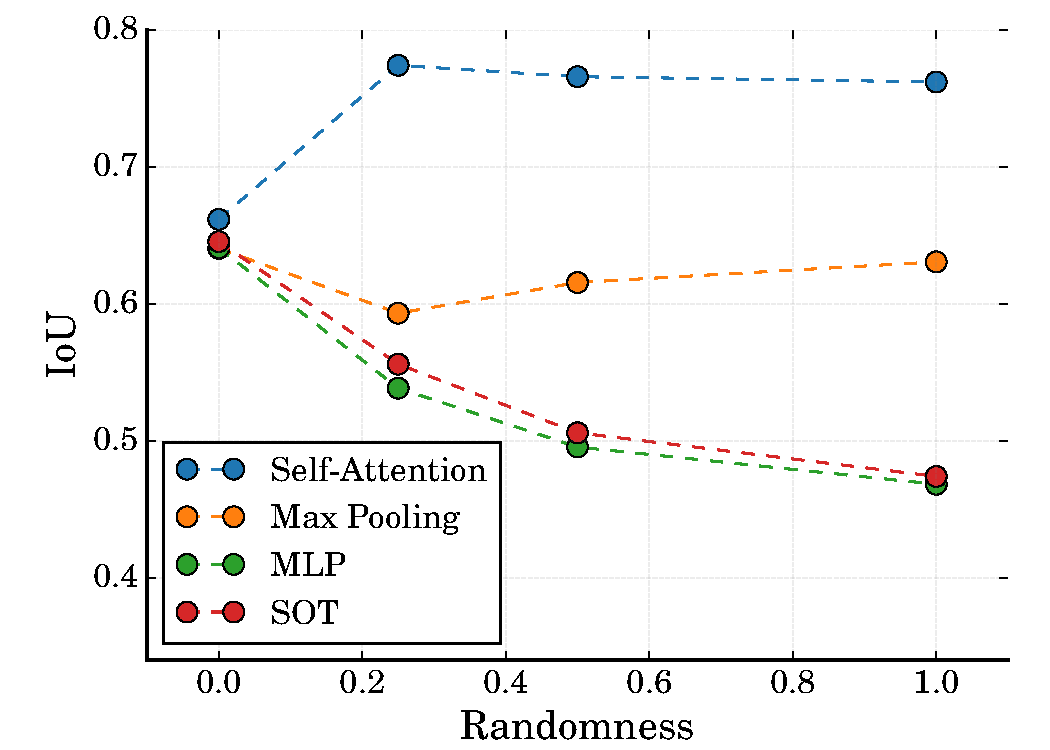
\includegraphics[width=\linewidth]{Figures/dial.pdf}
    \end{subfigure}
    \vspace{-2mm}
    \caption{
        Left: average IoU over sequence length for different implementations of relational reasoning on the toy domain shown in \cref{fig:toy2} ($\text{randomness} = 1.0$). Right: performance depending on how often agents are re-assigned identities randomly (sequence length 15). The higher the randomness, the less static the force field is and the more vital relational reasoning is. 
        \vspace{-4mm}
    }
    \label{fig:toy_quant}
\end{figure}

\Cref{fig:toy_quant} (left) shows a quantitative comparison of augmenting \textsc{hart} with different relational reasoning modules when identities are re-assigned in every timestep ($\text{randomness} = 1.0$). Exchanging information between trackers of different objects in the latent space with an MLP leads to slightly worse performance than the SOT baseline, while simple max-pooling performs significantly better ($\Delta \text{IoU} \sim 17\%$). This can be explained through the permutation invariance of the problem: the list of latent representation of the different objects has no meaningful order and the output of the model should therefore be invariant to the ordering of the objects. The MLP is in itself not permutation invariant and therefore prone to overfit to the (meaningless) order of the objects in the training data. Max-pooling, however, is permutation invariant and can in theory, despite its simplicity, be used to approximate any permutation invariant function - given a sufficiently large latent space \cite{Zaheer2017,Wagstaff2019}. Max-pooling is often used to exchange information between different tracklets, e.g., in the trajectory prediction domain \cite{social-lstm,Gupta2019}. However, self-attention, allowing for learned querying and encoding of information, solves the relational reasoning task significantly more accurately. In \Cref{fig:toy_quant} (right), the frequency with which object identities are reassigned randomly is varied. The results show that, in a deterministic environment, tracking does not necessarily profit from relational reasoning - even in the presence of long-range interactions. The less random, the more static the force field is and a static force field can be inferred from a small number of observations (see \Cref{fig:toy1}). This does of course not mean that all stochastic environments profit from relational reasoning. What these experiments indicate is that tracking can not be expected to profit from relational reasoning by default in any environment, but instead in environments which feature (potentially non-deterministic) dynamics and predictable interactions.
\section{Relational Reasoning in Real-World Tracking}
\label{sec:experiment_real}

\begin{figure}[ht!]
\centering
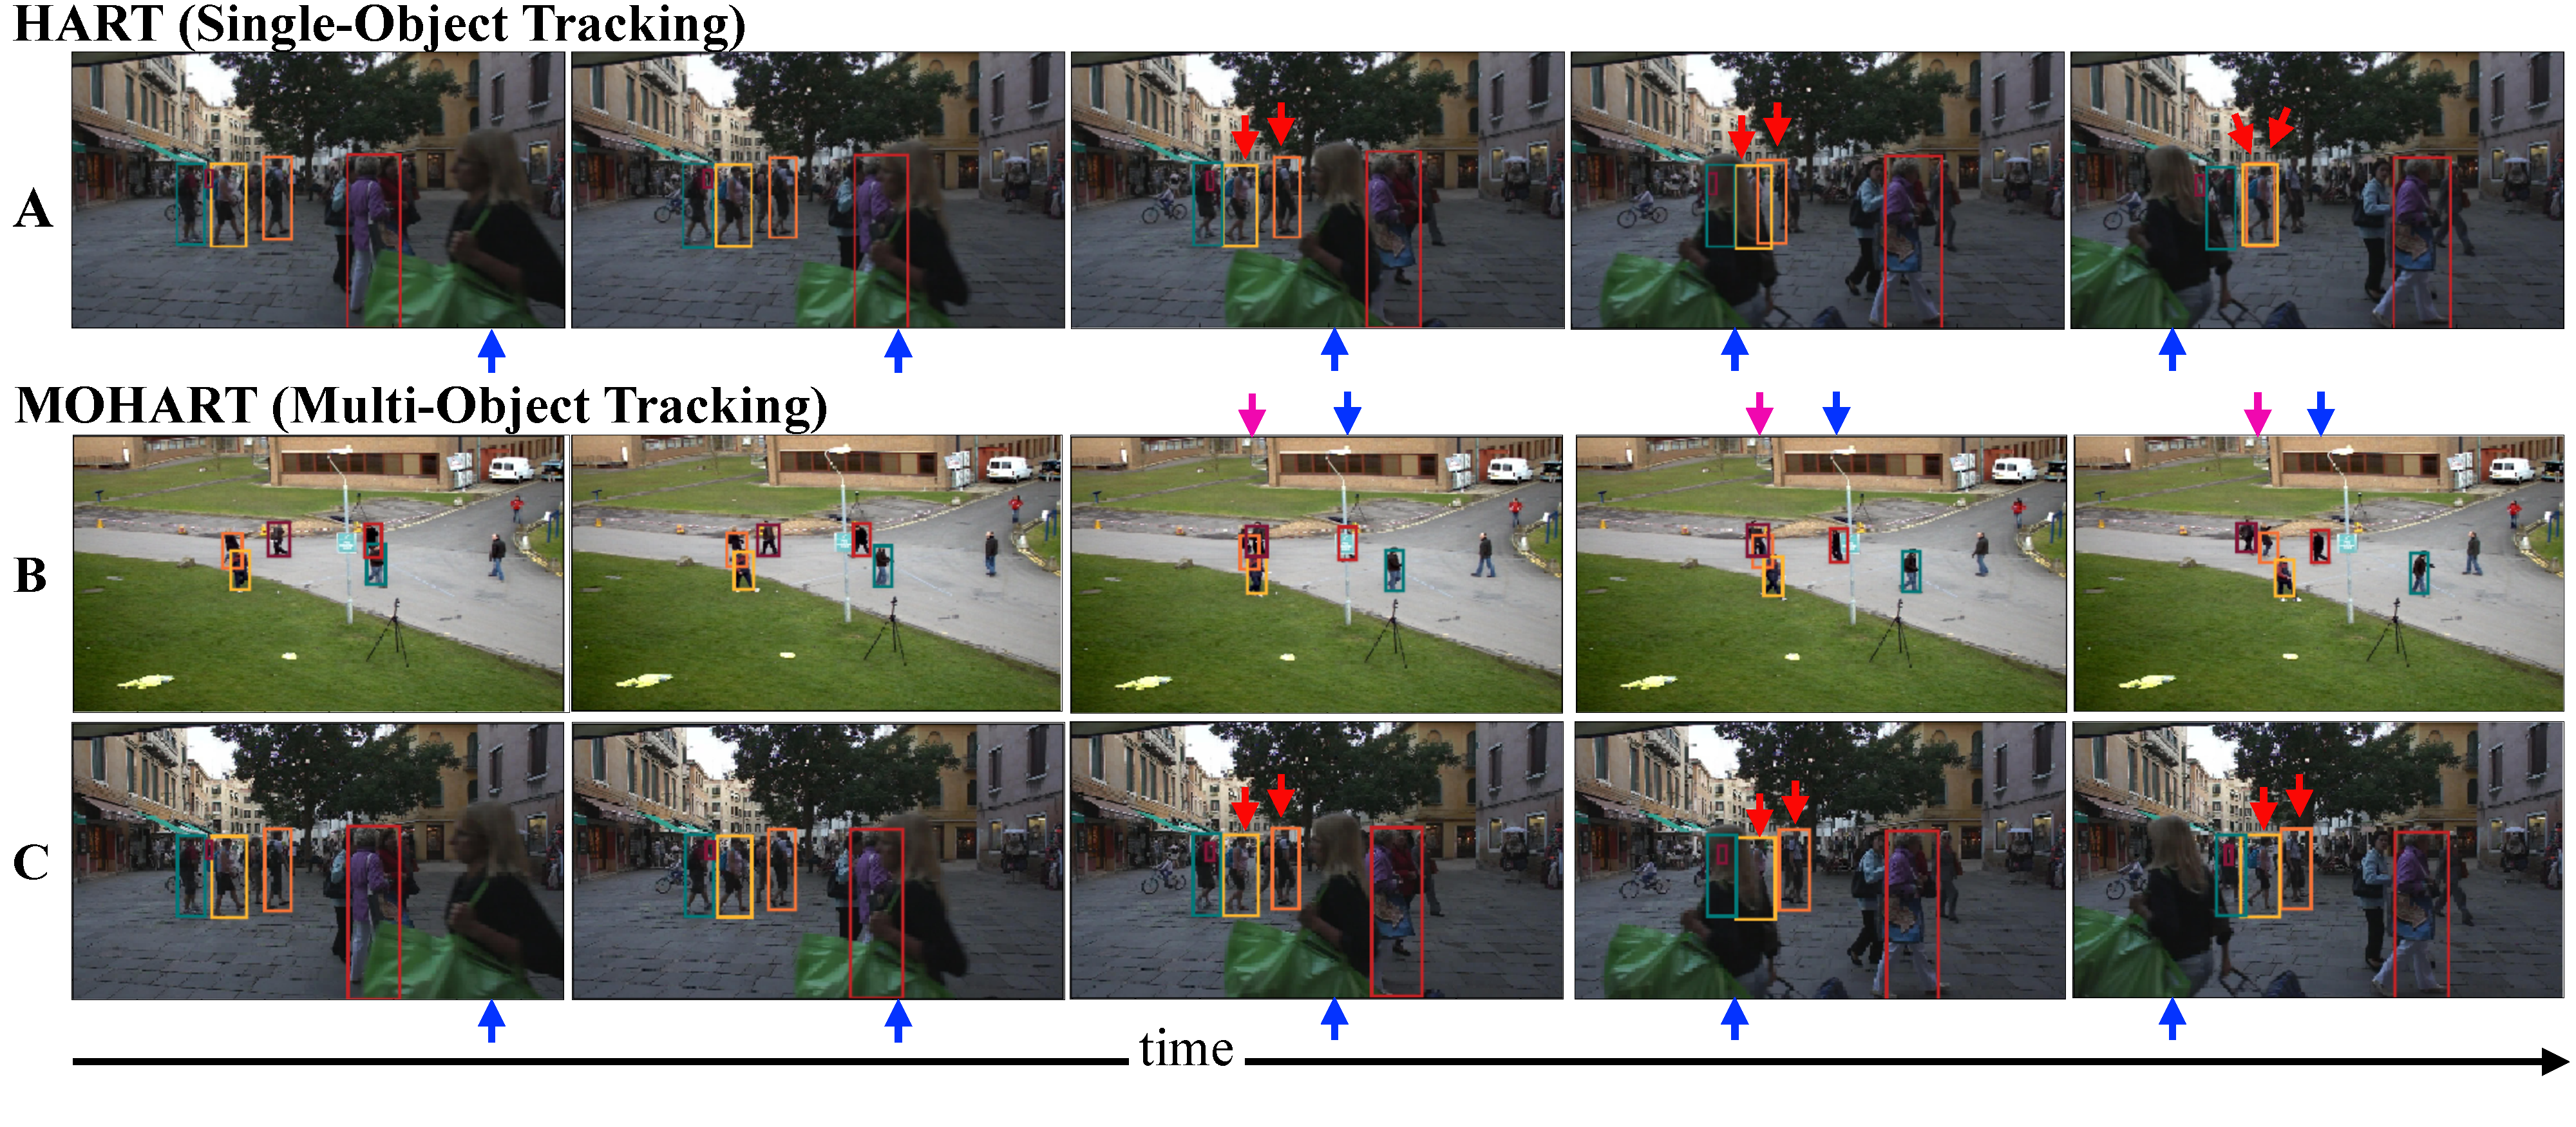
\includegraphics[width=1\textwidth]{figures/MOHART/tracking_qualitative}
\caption{Tracking examples of both \textsc{hart} and \textsc{mohart}. Coloured boxes are bounding boxes predicted by the model, arrows point at challenging aspects of the scenes. (A) \& (C): Each person being tracked is temporarily occluded by a woman walking across the scene (blue arrows). \textsc{mohart}, which includes a relational reasoning module, handles this more robustly (compare red arrows).}
\label{fig:tracking_and_predicting}
\end{figure}



Having established that \textsc{mohart} is capable of performing complex relational reasoning, we now test the algorithm on three real world datasets and analyse the effects of relational reasoning on performance depending on dataset and task. We find consistent improvements of \textsc{mohart} compared to \textsc{hart} throughout. Relational reasoning yields particularly high gains for scenes with ego-motion, crowded scenes, and simulated faulty sensor inputs.

\subsection{Experimental Details}
\label{sec:exp_details}

We investigate three qualitatively  different datasets: the MOTChallenge dataset \cite{MOT16}, the UA-DETRAC dataset \cite{Wen15}, and the Stanford Drone dataset \cite{DroneDataset}. In order to increase scene dynamics and make the tracking/prediction problems more challenging, we sub-sample some of the high framerate scenes with a stride of two. Training and architecture details are given in \Cref{sec:architecture_details} and \Cref{sec:experimental_details}.
We conduct experiments in three different modes:


\textbf{Tracking.} The model is initialised with the ground truth bounding boxes for a set of objects in the first frame. It then consecutively sees the following frames and predicts the bounding boxes. The sequence length is 30 time steps and the performance is measured as intersection over union (IoU) averaged over the entire sequence excluding the first frame. This algorithm is either applied to the entire dataset or subsets of it to study the influence of certain properties of the data.

\textbf{Camera Blackout.} This simulates unsteady or faulty sensor inputs. The setup is the same as in 
\textit{Tracking}, but sub-sequences images are blacked out. The algorithm is expected to recognise that no new information is available and that it should resort to its internal motion model.

\textbf{Prediction.} Testing \textsc{mohart}'s ability to capture motion patterns, only the first two frames are shown to the model followed by three black frames. IoU is measured seperately for each time step.



\begin{table}[!ht]
  \floatsetup{floatrowsep=qquad, captionskip=4pt}
        \ttabbox%
    {\begin{tabularx}{\textwidth}{l*{5}{>{\raggedleft\arraybackslash}X}}
      \toprule
&                   Entire &            Only &              No  &               Crowded &           Camera \\%[-0.4em]
&                   Dataset &           Ego-Motion &        Ego-Motion &        Scenes &            Blackout \\
      \midrule
\textbf{MOHART} &   \textbf{68.5\%} &   \textbf{66.9\%} &   \textbf{64.7\%} &   \textbf{69.1\%} &   \textbf{63.6\%}  \\[0.1em]
HART &              66.6\% &            64.0\% &            62.9\% &            66.9\% &            60.6\%  \\
\midrule
$\Delta$ &          1.9\% &             2.9\% &             1.8\% &             2.2\% &             3.0\%  \\ 
\bottomrule
      \addlinespace
      \addlinespace
      \addlinespace
      \end{tabularx}}
    {\caption{Tracking performance on the MOTChallenge dataset measured in IoU.}
      \label{tab:results_motc}}
  \begin{floatrow}[2]

      
    \ttabbox%
    {\begin{tabularx}{0.55\textwidth}{l*{3}{>{\raggedleft\arraybackslash}X}}
      \toprule
      & All & Crowded Scenes & Camera Blackout \\
      \midrule
      \textbf{MOHART} & 68.1\% & \textbf{69.5\%} & \textbf{64.2\%}\\
      [0.1em]
      HART & \textbf{68.4\%} & 68.6\% & 53.8\%\\
      \midrule
      $\Delta$ & -0.3\% & 0.9\% & 0.4\%\\
      \bottomrule
      \end{tabularx}}
    {\caption{UA-DETRAC Dataset}
      \label{tab:results_detrac}}
    \hfill%
    \ttabbox%
    {\begin{tabularx}{0.35\textwidth}{r*{3}{>{\raggedleft\arraybackslash}X}}
      \toprule
      All & Camera Blackout & CamBlack Bikes \\
      \midrule
      \textbf{57.3\%} & \textbf{52.6\%} & \textbf{53.3\%} \\
      [0.1em]
      56.1\% & 53.3\% & 50.7\%\\
      \midrule
      1.2\% & 0.7\% & 2.6\%\\
      \bottomrule
      \end{tabularx}}
    {\caption{Stanford Drone Dataset}
      \label{tab:results_stanford}}
  \end{floatrow}
\end{table}%



\subsection{Results and Analysis}


On the MOTChallenge dataset, \textsc{hart} achieves $66.6\%$ intersection over union (see \Cref{tab:results_motc}), which in itself is impressive given the small amount of training data of only 5225 training frames and no pre-training. \textsc{mohart} achieves $68.5\%$ (both numbers are averaged over 5 runs, independent samples $t$-test resulted in $p < 0.0001$). The performance gain increases when only considering ego-motion data. This is readily explained: movements of objects in the image space due to ego-motion scenarios are correlated and can therefore be better understood when combining information from movements of multiple objects, i.e. performing relational reasoning. In another ablation, we filtered for only crowded scenes by requesting five objects to be present for, on average, 90\% of the frames in a sub-sequence. For the MOT-Challenge dataset, this only leads to a minor increase of the performance gain of \textsc{mohart} indicating that the dataset exhibits a sufficient density of objects to learn interactions. The biggest benefit from relational reasoning can be observed in the \textit{camera blackout} experiments (setup explained in \Cref{sec:exp_details}). Both \textsc{hart} and \textsc{mohart} learn to rely on their internal motion models when confronted with black frames and propagate the bounding boxes according to the previous movement of the objects. It is unsurprising that this scenario profits particularly from relational reasoning. Qualitative tracking and \textit{camera blackout} results are shown in \Cref{fig:tracking_and_predicting} and in \Cref{sec:blackout}, respectively.

Tracking performance on the UA-DETRAC dataset only profits from relational reasoning when filtering for crowded scenes (see \Cref{tab:results_detrac}). The fact that the performance of \textsc{mohart} is slightly worse on the vanilla dataset ($\Delta = -0.3\%$) can be explained with more overfitting. As there is no exchange between trackers for each object, each object constitutes an independent training sample.

The Stanford drone dataset (see \Cref{tab:results_stanford}) is qualitatively different to the other two as it is filmed from a top down view. The scenes are more crowded and each object only covers a small number of pixels rendering it a difficult problem for tracking. The dataset was designed for trajectory prediction, a problem setup where an algorithm is typically provided with ground truth tracklets in coordinate space and potentially an image as context information. The task is then to extrapolate these tracklets into the future. The tracking performance profits from relational reasoning more than on the UA-DETRAC dataset but less than on the MOTChallenge dataset. The performance gain on the \textit{camera blackout} experiments are particularly strong when only considering cyclists. 


\begin{figure}
    \centering
    \begin{subfigure}[c]{0.99\linewidth}
        \centering
        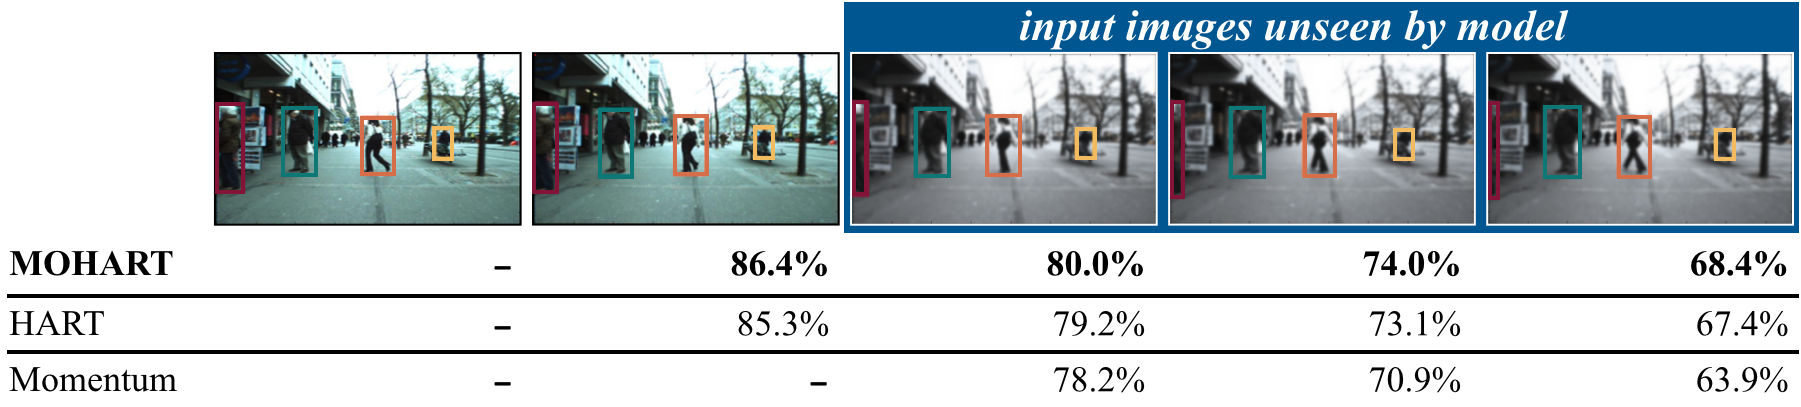
\includegraphics[width=\linewidth]{figures/MOHART/prediction_motc2.png}
        \caption{Prediction results on the MOTChallenge dataset \cite{MOT16}.}
        \label{fig:MOTC_imgs}
    \end{subfigure}
    \begin{subfigure}[c]{0.99\linewidth}
        \centering
        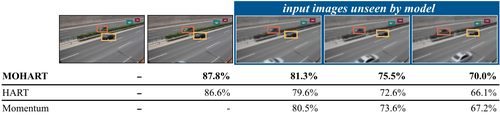
\includegraphics[width=\linewidth]{figures/MOHART/prediction_detrac2.png}
        \caption{Prediction results on the UA-DETRAC dataset (crowded scenes only) \cite{Wen15}.}
        \label{fig:Detrac_quant}
    \end{subfigure}
\caption{Peeking into the future. Only the first two frames are shown to the tracking algorithm followed by three black frames. \textsc{mohart} learns to fall back on its internal motion model when no observation (i.e. only a black frame) is available. The reported IoU scores show the performance for the respective frames 0, 1, 2, and 3 time steps into the future.
\label{fig:prediction}
}
\end{figure}

In the results from the \textit{prediction} experiments (see \Cref{fig:prediction}) \textsc{mohart} consistently outperforms \textsc{hart}. On both datasets, the model outperforms a baseline which uses momentum to linearly extrapolate the bounding boxes from the first two frames. This shows that even from just two frames, the model learns to capture motion models which are more complex than what could be observed from just the bounding boxes (i.e. momentum), suggesting that it uses visual information (\textsc{hart} \& \textsc{mohart}) as well as relational reasoning (\textsc{mohart}). The strong performance gain of \textsc{mohart} compared to \textsc{hart} on the UA-DETRAC dataset, despite the small differences for tracking on this dataset, can be explained as follows: this dataset features little interactions but strong correlations in motion. Hence when only having access to the first two frames, \textsc{mohart} profits from estimating the velocities of multiple cars simultaneously.

%\vspace*{-1em}
\section{Conclusion}
%\vspace*{-1em}
\label{sec:mohart_discussion}

With MOHART, we introduce an end-to-end multi-object tracker that is capable of capturing complex interactions and leveraging these for precise predictions as experiments both on toy and real world data show. However, the experiments also show that the benefit of relational reasoning strongly depends on the nature of the data. The toy experiments showed that in an entirely deterministic world relational reasoning was much less important than in a stochastic environment. Amongst the real-world dataset, the highest performance gains from relational reasoning were achieved on the MOTChallenge dataset, which features crowded scenes, ego-motion and occlusions.



\section*{Acknowledgements}
We thank Stefan Saftescu for his contributions, particularly for integrating the Stanford Drone Dataset, and Adam Golinski as well as Stefan Saftescu for proof-reading. This research was funded by the EPSRC AIMS Centre for Doctoral Training at Oxford University and an EPSRC Programme Grant (EP/M019918/1).
We acknowledge use of Hartree Centre resources in this work. The STFC Hartree Centre is a research collaboratory in association with IBM providing High Performance Computing platforms funded by the UK's investment in e-Infrastructure. The Centre aims to develop and demonstrate next generation software, optimised to take advantage of the move towards exa-scale computing.

\begin{subappendices}
	\begin{figure}
	\centering
	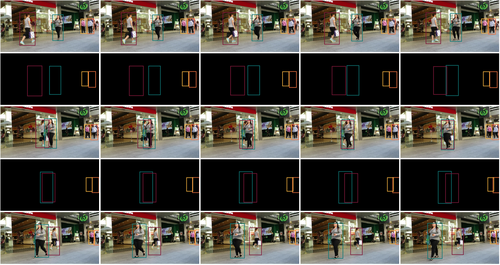
\includegraphics[width=1.0\textwidth]{figures/MOHART/mot_example1.png}
	\vspace{-6mm}
	\caption{Camera blackout experiment on a pedestrian street scene from the MOTChallenge dataset without ego-motion. Subsequent frames are displayed going from top left to bottom right. Shown are the inputs to the model (some of them being black frames, i.e. arrays of zeroes) and bounding boxes predicted by \textsc{MOHART} (coloured boxes). This scene is particularly challenging as occlusion and missing sensor input coincide (fourth row).
	\vspace{-2mm}}
	\label{fig:blackout1}
\end{figure}
\section{Architecture Details}
\label{sec:architecture_details}
The architecture details were chosen to optimise \textsc{hart} performance on the MOTChallenge dataset. They deviate from the original \textsc{hart} implementation \cite{Kosiorek17} as follows: The presence variable is predicted with a binary cross entropy loss. The maximum number of objects to be tracked simultaneously was set to 5 for the UA-DETRAC and MOTChallenge dataset. For the more crowded Stanford drone dataset, this number was set to 10. The feature extractor is a three layer convolutional network with a kernel size of 5, a stride of 2 in the first and last layer, 32 channels in the first two layers, 64 channels in the last layer, ELU activations, and skip connections. This converts the initial $32 \times 32 \times 3$ glimpse into a $7 \times 7 \times 64$ feature representation. This is followed by a fully connected layer with a 128 dimensional output and an elu activation. The spatial attention parameters are linearly projected onto 128 dimensions and added to this feature representation serving as a positional encoding. The LSTM has a hidden state size of 128. The self-attention unit in \textsc{mohart} comprises linear projects the inputs to dimensionality 128 for each keys, queries and values. For the real-world experiments, in addition to the extracted features from the glimpse, the hidden states from the previous LSTM state are also fed as an input by concatinating them with the features. In all cases, the output of the attention module is concatenated to the input features of the respective object.

As an optimizer, we used RMSProp with momentum set to $0.9$ and learning rate $5*10^{-6}$. For the MOTChallenge dataset and the UA-DETRAC dataset, the models were trained for 100,000 iterations of batch size 10 and the reported IoU is exponentially smoothed over iterations to achieve lower variance. For the Stanford Drone dataset, the batch size was increased to 32, reducing time to convergence and hence model training to 50,000 iterations.

\section{Experimental Details}
\label{sec:experimental_details}
The MOTChallenge and the UA-DETRAC dataset discussed in this section are intended to be used as a benchmark suite for multi-object-tracking in a tracking-by-detection paradigm. Therefore, ground truth bounding boxes are only available for the training datasets. The user is encouraged to upload their model which performs tracking in a data association paradigm leveraging the provided bounding box proposals from an external object detector. As we are interested in a different analysis (IoU given inital bounding boxes), we divide the training data further into training and test sequences. To make up for the smaller training data, we extend the MOTChallenge 2017 dataset with three sequences from the 2015 dataset (ETH-Sunnyday, PETS09-S2L1, ETH-Bahnhof). We use the first 70\% of the frames of each of the ten sequences for training and the rest for testing. Sequences with high frame rates (30Hz) are sub-sampled with a stride of two. For the UA-DETRAC dataset, we split the 60 available sequences into 44 training sequences and 16 test sequences. For the considerably larger Stanford Drone dataset we took three videos of the scene \textit{deathCircle} for training and the remaining two videos from the same scene for testing. The videos of the drone dataset were also sub-sampled with a stride of two to increase scene dynamics.


\section{Camera Blackout Experiments}
\label{sec:blackout}

\begin{figure}
	\centering
	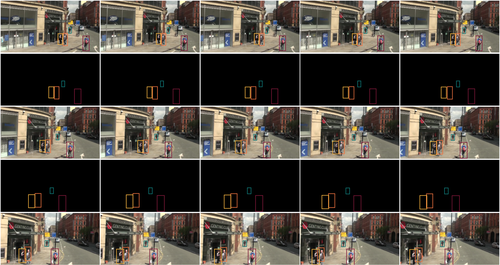
\includegraphics[width=1.0\textwidth]{figures/MOHART/mot_example2.png}
	\vspace{-6mm}
	\caption{Camera blackout experiment on a street scene from the MOTChallenge dataset with strong ego-motion. The reader is encouraged to compare top left and bottom right frame to make the amount of ego-motion apparent.}
	\label{fig:blackout2}
\end{figure}


In \Cref{sec:experiment_real}, we conducted a set of camera blackout experiments to test \textsc{mohart}'s capability of dealing with faulty sensor inputs. While traditional pipeline methods require careful consideration of different types of corner cases to properly handle erroneous sensor inputs, \textsc{mohart} is able to capture these automatically, especially when confronted with similar issues in the training scenarios. To simulate this, we replace subsequences of the images with black frames. \Cref{fig:blackout1} and \Cref{fig:blackout2} show two such examples from the test data together with the model's prediction. \textsc{mohart} learns not to update its internal model when confronted with black frames and instead uses the LSTM to propagate the bounding boxes. When proper sensor input is available again, the model uses this to make a rapid adjustment to its predicted location and `snap' back onto the object. This works remarkably well in both the presence of occlusion (\Cref{fig:blackout1}) and ego-motion (\Cref{fig:blackout2}). \Cref{tab:results_motc,tab:results_detrac,tab:results_stanford} show that the benefit of relational reasoning is particularly high in these scenarios specifically. These experiments can also be seen as a proof of concept of \textsc{mohart}'s capabalities of predicting future trajectories---and how this profits from relational reasoning.
\end{subappendices}

\chapter{Sequential Attend, Infer, Repeat: Generative Modelling of Moving Objects}
\label{ch:sqair}


%\begin{abstract}
\vspace{-5pt}
We present Sequential Attend, Infer, Repeat (\textsc{sqair}), an interpretable deep generative model for videos of moving objects.
It can reliably discover and track objects throughout the sequence of frames, and can also generate future frames conditioning on the current frame, thereby simulating expected motion of objects. 
This is achieved by explicitly encoding object presence, locations and appearances in the latent variables of the model.
\textsc{Sqair} retains all strengths of its predecessor, Attend, Infer, Repeat (\textsc{air}, \cite{Eslami2016}), including learning in an unsupervised manner, and addresses its shortcomings.
We use a moving multi-\textsc{mnist} dataset to show limitations of AIR in detecting overlapping or partially occluded objects, and show how \textsc{sqair} overcomes them by leveraging temporal consistency of objects.
Finally, we also apply \textsc{sqair} to real-world pedestrian CCTV data, where it learns to reliably detect, track and generate walking pedestrians with no supervision.
\end{abstract}
\section{Introduction}
\label{sec:intro}

The ability to identify objects in their environments and to understand relations between them is a cornerstone of human intelligence \citep{Kemp2008discovery}. Arguably, in doing so we rely on a notion of spatial and temporal consistency which gives rise to an expectation that objects do not appear out of thin air, nor do they spontaneously vanish, and that they can be described by properties such as location, appearance and some dynamic behaviour that explains their evolution over time. We argue that this notion of consistency can be seen as an \textit{inductive bias} that improves the efficiency of our learning. Equally, we posit that introducing such a bias towards spatio-temporal consistency into our models should greatly reduce the amount of supervision required for learning.

One way of achieving such inductive biases is through model structure. 
While recent successes in deep learning demonstrate that progress is possible without explicitly imbuing models with interpretable structure \citep{Lecun2015deep}, recent works show that introducing such structure into deep models can indeed lead to favourable inductive biases improving performance  e.g.\ in convolutional networks \citep{Lecun1989backpropagation} or in tasks requiring relational reasoning \citep{Santoro2017}.
Structure can also make neural networks useful in new contexts by significantly improving generalization, data efficiency \citep{Jacobsen2016struc} or extending their capabilities to unstructured inputs \citep{Graves2016}.

\gls{AIR}, introduced by \cite{Eslami2016}, is a notable example of such a structured probabilistic model that relies on deep learning and admits efficient amortized inference.
Trained without any supervision, \gls{AIR} is able to decompose a visual scene into its constituent components and to generate a (learned) number of latent variables that explicitly encode the location and appearance of each object. While this approach is inspiring, its focus on modelling individual (and thereby inherently static) scenes leads to a number of limitations. For example, it often merges two objects that are close together into one since no temporal context is available to distinguish between them. Similarly, we demonstrate that \gls{AIR} struggles to identify partially occluded objects, e.g.\ when they extend beyond the boundaries of the  scene frame (see \Cref{fig:partial_glimpse} in \Cref{sec:expr_mnist}). 

Our contribution is to mitigate the shortcomings of  \gls{AIR} by introducing a sequential version that models sequences of frames, enabling it to discover and track objects over time as well as to generate convincing extrapolations of frames into the future. We achieve this by leveraging temporal information to learn a richer, more capable generative model. Specifically, we extend \gls{AIR} into a spatio-temporal state-space model and train it on unlabelled image sequences of dynamic objects. 
We show that the resulting model, which we name Sequential \gls{AIR} (\acrshort{SQAIR}), retains the strengths of the original AIR formulation while outperforming it on moving \gls{MNIST} digits.

The rest of this work is organised as follows.
In \Cref{sec:air}, we describe the generative model and inference of \gls{AIR}.
In \Cref{sec:sqair}, we discuss its limitations and how it can be improved, thereby introducing \gls{SQAIR}, our extension of \gls{AIR} to image sequences.
In \Cref{sec:experiments}, we demonstrate the model on a dataset of multiple moving MNIST digits (\Cref{sec:expr_mnist}) and compare it against \gls{AIR} trained on each frame and \gls{VRNN} of \cite{Chung2015} with convolutional architectures, and show the superior performance of \gls{SQAIR} in terms of log marginal likelihood and interpretability of latent variables.
We also investigate the utility of inferred latent variables of \gls{SQAIR} in downstream tasks.
In \Cref{sec:expr_duke} we apply \gls{SQAIR} on real-world pedestrian CCTV data, where \gls{SQAIR} learns to reliably detect, track and generate walking pedestrians without any supervision.
Code for the implementation on the \textsc{mnist} dataset\footnote{code: \href{https://github.com/akosiorek/sqair}{github.com/akosiorek/sqair}} and the results video\footnote{video: \href{https://youtu.be/-IUNQgSLE0c}{youtu.be/-IUNQgSLE0c}} are available online.
\section{Attend, Infer, Repeat (\textsc{AIR})}
\label{sec:air}

% recap of AIR
\gls{AIR}, introduced by \cite{Eslami2016}, is a structured \gls{VAE} capable of decomposing a static scene $\bx$ into its constituent objects, where each object is represented as a separate triplet of continuous latent variables $\bz = \{\bz^{\mathrm{what}, i}, \bz^{\mathrm{where}, i}, z^{\mathrm{pres},i}\}_{i=1}^n$, $n \in \mathbb{N}$ being the (random) number of objects in the scene.
Each triplet of latent variables explicitly encodes position, appearance and presence of the respective object, and the model is able to infer the number of objects present in the scene. Hence it is able to count, locate and describe objects in the scene, all learnt in an unsupervised manner, made possible by the inductive bias introduced by the model structure.

\textbf{Generative Model}
The generative model of \gls{AIR} is defined as follows
\begin{align}
\label{eq:air_gen}
    \p{n}{}{\theta} &= \mathrm{Geom} (n \mid \theta), 
    &
    \p{\bz^{\mathrm{w}}}{n}{\theta} &= \prod_{i=1}^n \p{\bz^{w,i}}{}{\theta} = \prod_{i=1}^n \gauss{\bz^{w,i}|\bf{0}, \bf{I}},\nonumber \\
    \p{\bx}{\bz}{\theta} &= \gauss{\bx \mid \byt, \sigma^2_x \bm{I}}, 
    &\text{with}~~\byt &= \sum_{i=1}^n \operatorname{h}^\mathrm{dec}_\theta (
        \bz^{\mathrm{what}, i}, \bz^{\mathrm{where}, i}
    ),
\end{align}
where $\bz^{\mathrm{w},i} \defeq (\bz^{\mathrm{what}, i}, \bz^{\mathrm{where}, i})$, $z^{\mathrm{pres}, i}=1$ for $i=1 \ldots n$ and $h^\mathrm{dec}_\theta$ is the object decoder with parameters $\theta$.
It is composed of a \textit{glimpse decoder} $f_\theta^\mathrm{dec}: \bgt^i \mapsto \byt^i$,
which constructs an image patch and a 
spatial transformer ($\operatorname{ST}$, \cite{Jaderberg2015}), which scales and shifts it according to $\bz^\mathrm{where}$; see \Cref{fig:generation} for details.

\textbf{Inference}
\cite{Eslami2016} use a sequential inference algorithm, where latent variables are inferred one at a time; see \Cref{fig:sqair_inf_flow}.
The number of inference steps $n$ is given by $z^{\mathrm{pres}, 1:n+1}$, a random vector of $n$ ones followed by a zero. The $\bz^{i}$ are sampled sequentially from
\vspace{-7pt}
\begin{equation} \label{eq:air_posterior}
    \q{\bz}{\bx}{\phi} = 
        \q{z^{\mathrm{pres}, n+1} = 0}{\bz^{\mathrm{w}, 1:n}, \bx}{\phi} 
        \prod_{i=1}^n 
        \q{\bz^{\mathrm{w}, i}, z^{\mathrm{pres}, i} = 1}{\bz^{1:i-1}, \bx}{\phi},
\end{equation}
where $q_\phi$ is implemented as a neural network with parameters $\phi$. 
To implement explaining away, e.g.\ to avoid encoding the same object twice, it is vital to capture the dependency of $\bz^{\mathrm{w},i}$ and  $z^{\mathrm{pres}, i}$ on $\bz^{1:i-1}$ and $\bx$. This is done using a \gls{RNN} $R_\phi$ with hidden state $\bm{h}^i$, namely:
$
    \bm{\omega}^i, \bm{h}^i = R_\phi (\bx, \bz^{i-1}, \bm{h}^{i-1}).
$
The outputs $\bm{\omega}^i$, which are computed iteratively and depend on the previous latent variables (\textit{cf}. \Cref{algo:sqair_disc}), parametrise $\q{\bz^{\mathrm{w},i}, \bz^{\mathrm{pres},i}}{\bz^{1:i-1}, \bx}{\phi}$. For simplicity the latter is assumed to factorise such that
$
    \q{\bz^{\mathrm{w}}, \bz^{\mathrm{pres}}}{\bz^{1:i-1}, \bx}{\phi} = \q{z^{\mathrm{pres}, n+1} = 0}{\bm{\omega}^{n+1}}{\phi} \prod_{i=1}^n \q{\bz^{\mathrm{w},i}}{\bm{\omega}^i}{\phi} \q{z^{\mathrm{pres}, i} = 1}{\bm{\omega}^i}{\phi}.
$

\begin{figure}
    \centering
    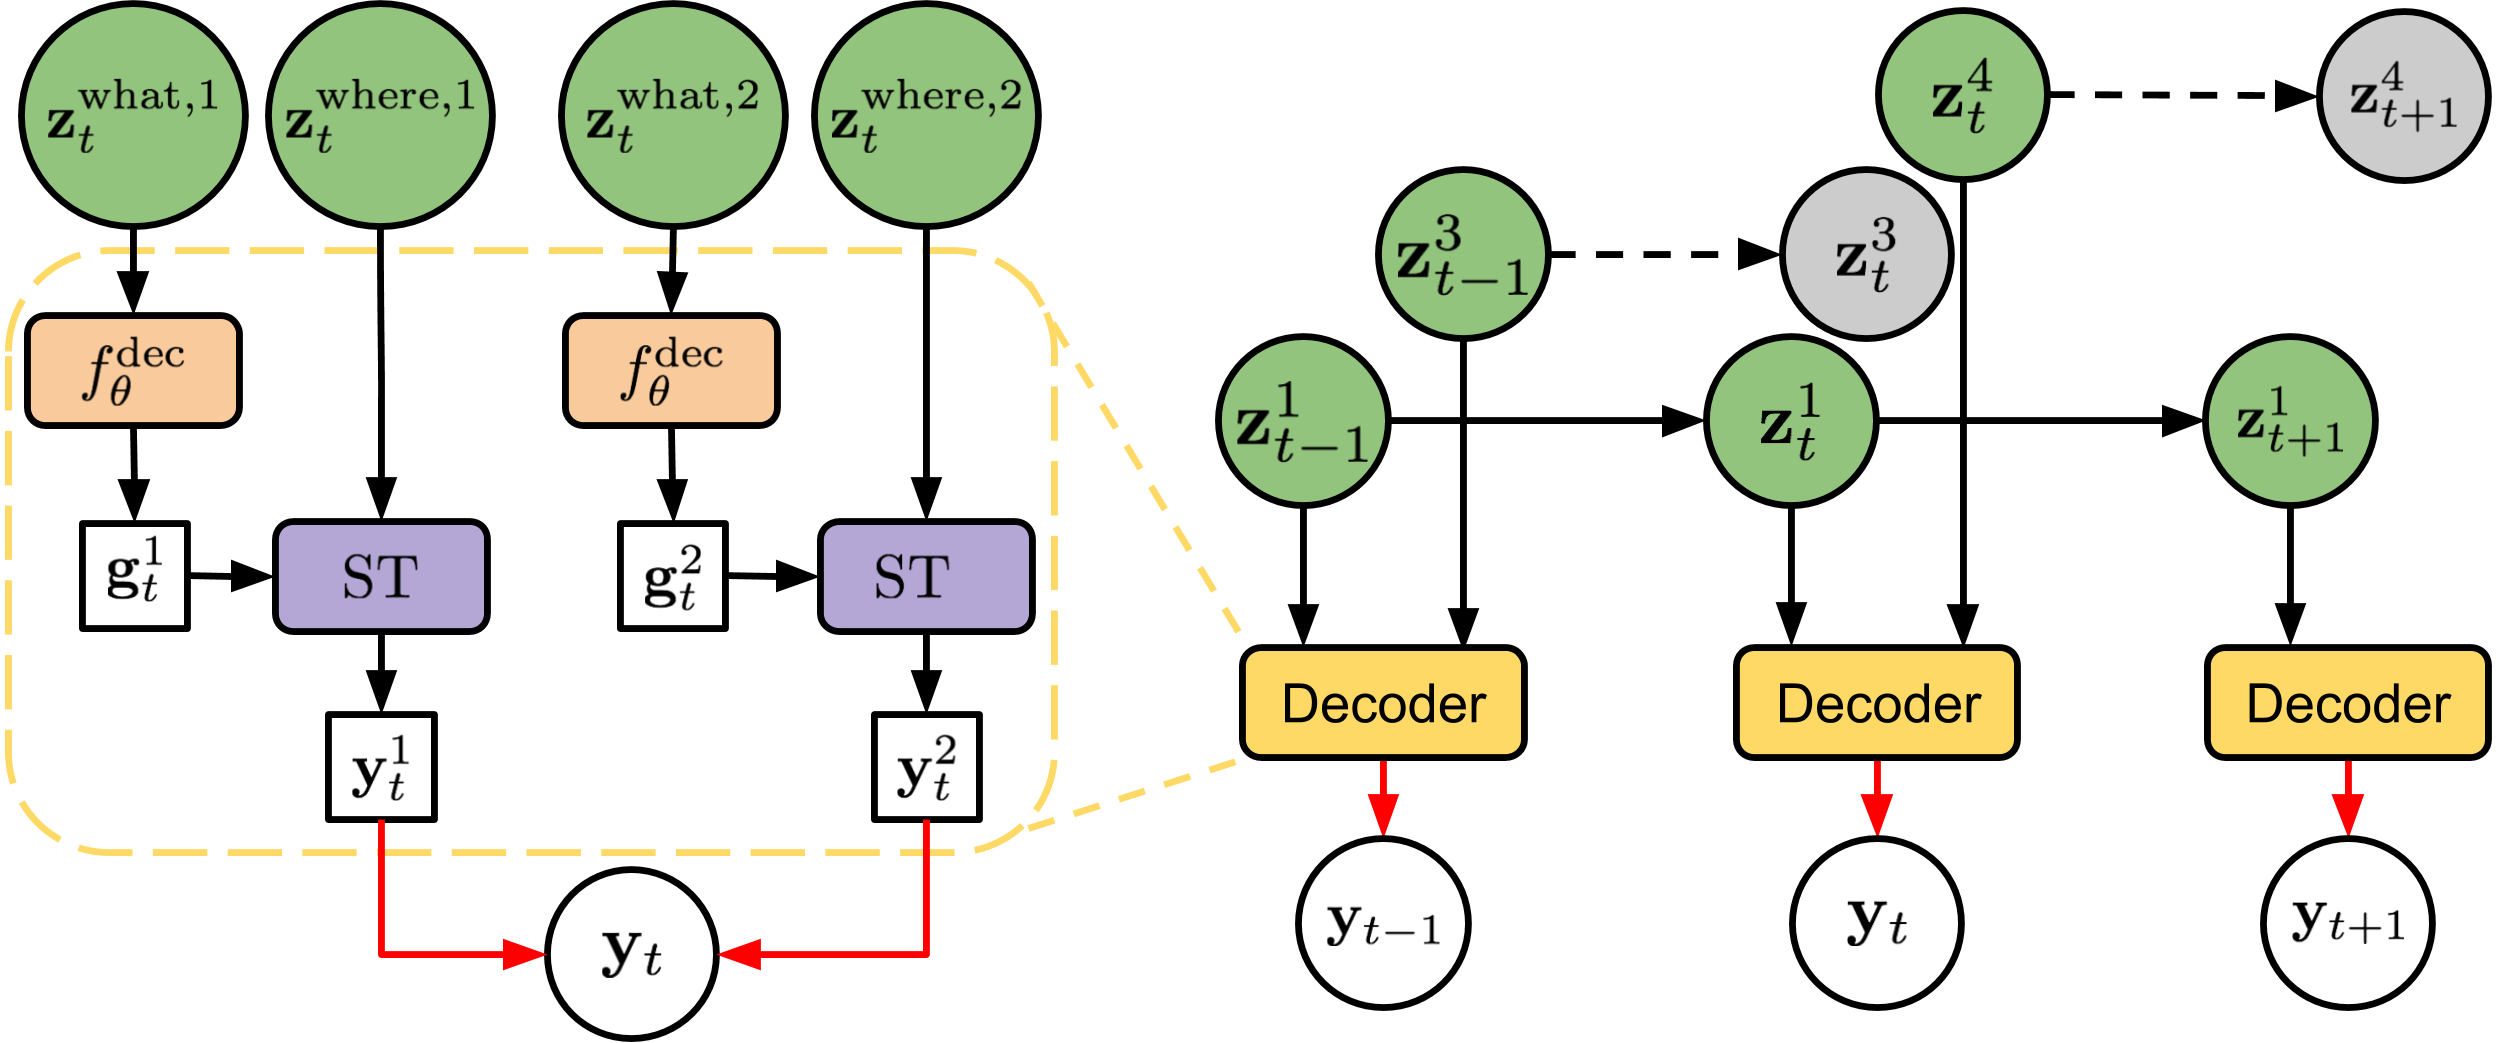
\includegraphics[width=0.7\linewidth]{figures/SQAIR/air_sqair_generation}
    \caption{
        \textit{Left}:
            Generation in \gls{AIR}.
            The image mean $\byt$ is generated by first using the \textit{glimpse decoder} $f_\theta^\mathrm{dec}$ to map the \textit{what} variables into glimpses $\bgt$, transforming them with the \textit{spatial transformer} $\STN$ according to the \textit{where} variables and summing up the results.
        \textit{Right}:
            Generation in \gls{SQAIR}.
%            When new objects enter the frame, new latent variables (here, $\bzt^4$) are sampled from the \textit{discovery} prior. The temporal evolution of already present objects is governed by the \textit{propagation} prior, which can choose to forget some variables (here, $\bzt^3$ and $\bz_{t+1}^4$) when the object moves out of the frame. The image generation process, which mimics the left-hand side of the figure, is abstracted in the \textit{decoder} block. 
    }
    \label{fig:generation}
\end{figure}


\section{Sequential Attend-Infer-Repeat}
\label{sec:sqair}

\begin{figure}
    \centering
    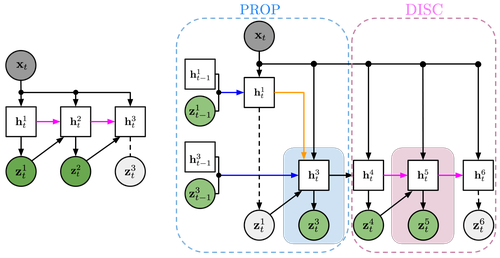
\includegraphics[width=.7\linewidth]{figures/SQAIR/air_sqair_inference}
    \caption{
    \textit{Left}: 
        Inference in \gls{AIR}. 
        The \textcolor{pink}{pink \gls{RNN}} attends to the image sequentially and produces one latent variable $\bzt^i$ at a time. 
        Here, it decides that two latent variables are enough to explain the image and $\bzt^3$ is not generated.
    % 
    \textit{Right}:
        Inference in \gls{SQAIR} starts with the \gls{prop} phase.
        \gls{prop} iterates over latent variables from the previous time-step $t-1$ and updates them based on the new observation $\bxt$.
        The \textcolor{blue}{blue \gls{RNN}} runs forward in time to update the hidden state of each object, to model its change in appearance and location throughout time. 
        The \textcolor{orange}{orange \gls{RNN}} runs across all current objects and models the relations between different objects.
        Here, when attending to $\bz^1_{t-1}$, it decides that the corresponding object has disappeared from the frame and \textit{forgets} it.
        Next, the \gls{disc} phase detects new objects as in \gls{AIR}, but in \gls{SQAIR} it is also conditioned on the results of \gls{prop}, to prevent rediscovering objects. See \Cref{fig:sqair_inf_detail} for details of the colored \glspl{RNN}.}
    \label{fig:sqair_inf_flow}
\end{figure}


While capable of decomposing a scene into objects, \gls{AIR} only describes single images. Should we want a similar decomposition of an image sequence, it would be desirable to do so in a temporally consistent manner. For example, we might want to detect objects of the scene as well as infer dynamics and track identities of any persistent objects.
Thus, we introduce  \glsreset{SQAIR} \gls{SQAIR}, whereby \gls{AIR} is augmented with a \gls{SSM} to achieve temporal consistency in the generated images of the sequence.
The resulting probabilistic model is composed of two parts:  \glsreset{disc}\gls{disc}, which is responsible for detecting  (or introducing, in the case of the generation) new objects at every time-step (essentially equivalent to \gls{AIR}), and \glsreset{prop}\gls{prop}, responsible for updating (or forgetting) latent variables from the previous time-step given the new observation (image), effectively implementing the temporal \gls{SSM}.
We now formally introduce \gls{SQAIR} by first describing its generative model and then the inference network.

\textbf{Generative Model}
The model assumes that at every-time step, objects are first propagated from the previous time-step (\gls{prop}). Then, new objects are introduced (\gls{disc}). 
Let $t \in \mathbb{N}$ be the current time-step.
Let $\mathcal{P}_t$ be the set of objects propagated from the previous time-step and let $\mathcal{D}_t$ be the set of objects discovered at the current time-step, and let $\mathcal{O}_t = \mathcal{P}_t \cup \mathcal{D}_t$ be the set of all objects present at time-step~$t$.
% Let $P_t \defeq |\mathcal{P}_t|$ and $D_t \defeq |\mathcal{D}_t|$.
Consequently, at every time step, the model retains a set of latent variables $\bzt^{\mathcal{P}_t} = \{ \bzt^i \}_{i \in \mathcal{P}_t}$, and generates a set of new latent variables $\bzt^{\mathcal{D}_t} = \{ \bzt^i \}_{i \in \mathcal{D}_t}$. Together they form $\bzt \defeq [\bzt^{\mathcal{P}_t}, \bzt^{\mathcal{D}_t}]$, where the representation of the $i^\mathrm{th}$ object $\bzt^i \defeq [ \bzt^{\mathrm{what}, i}, \bzt^{\mathrm{where}, i}, \zt^{\mathrm{pres}, i}]$ is composed of three components (as in \gls{AIR}): 
$\bzt^{\mathrm{what},i}$ and $\bzt^{\mathrm{where},i}$ are real vector-valued variables representing appearance and location of the object, respectively. $\zt^{\mathrm{pres},i}$ is a binary variable representing whether the object is present at the given time-step or not.

At the first time-step ($t = 1$) there are no objects to propagate, so we sample $D_1$, the number of objects at $t=1$, from the discovery prior $\pd{D_1}{}{}$. 
Then for each object $i \in \mathcal{D}_t$, we sample latent variables $\bzt^{\mathrm{what}, i}, \bzt^{\mathrm{where}, i}$ from $\pd{z_1^i}{D_1}{}$. 
At time $t=2$, the \textit{propagation} step models which objects from $t=1$ are propagated to $t=2$, and which objects disappear from the frame, using the binary random variable $(\zt^{\mathrm{pres},i})_{i \in \mathcal{P}_t}$. 
The \textit{discovery} step at $t=2$ models new objects that enter the frame, with a similar procedure to $t=1$: sample $D_2$ (which depends on $\bz_2^{\mathcal{P}_2}$) then sample $(\bz_2^{\mathrm{what}, i}, \bz_2^{\mathrm{where}, i})_{i\in \mathcal{D}_2}$. 
This procedure of propagation and discovery recurs for $t = 2, \ldots T$.
Once the $\bzt$ have been formed, we may generate images $\bxt$ using the exact same generative distribution $\p{\bxt}{\bzt}{\theta}$ as in \gls{AIR} (\textit{cf}. \Cref{eq:air_gen,fig:generation,algo:air_decoding}). 
In full, the generative model is:
\begin{equation} \label{eq:full_joint}
p(\bx_{1:T},\bz_{1:T},D_{1:T}) 
    = \pd(D_1,\bz_1^{\mathcal{D}_1}) \prod_{t=2}^T \pd(D_t,\bzt^{\mathcal{D}_t}|\bzt^{\mathcal{P}_t})\pp(\bzt^{\mathcal{P}_t}|\bz_{t-1}) p_{\theta}(\bxt|\bzt),
\end{equation}
The \textit{discovery prior} $\pd(D_t,\bzt^{\mathcal{D}_t}|\bzt^{\mathcal{P}_t})$ samples latent variables for new objects that enter the frame. The \textit{propagation prior} $\pp(\bzt^{\mathcal{P}_t}|\bz_{t-1})$ samples latent variables for objects that persist in the frame and removes latents of objects that disappear from the frame, thereby modelling dynamics and appearance changes. Both priors are learned during training. The exact forms of the priors are given in \Cref{apd:sqair_generation}.
\begin{figure}
    \centering
    \begin{minipage}[c]{0.49\linewidth}
        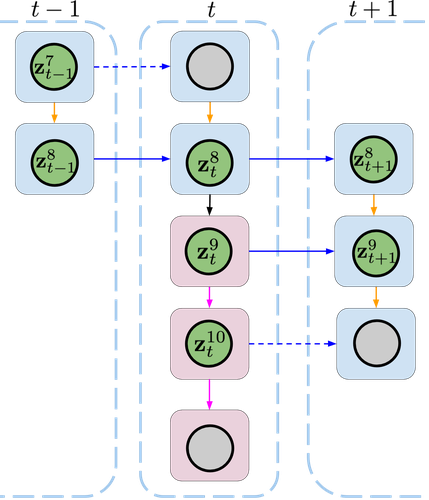
\includegraphics[width=\linewidth]{figures/SQAIR/diagrams/sqair_flow_plus_prop_simple}
    \end{minipage}
    \hfill
    \begin{minipage}[c]{0.49\linewidth}
    \caption{
        \textit{Left}:
            Interaction between \gls{prop} and \gls{disc} in \gls{SQAIR}.
            Firstly, objects are propagated to time $t$, and object $i=7$ is dropped.
            Secondly, \gls{disc} tries to discover new objects.
            Here, it manages to find two objects: $i=9$ and $i=10$.
            The process recurs for all remaining time-steps.
            \textcolor{blue}{Blue arrows} update the temporal hidden state, \textcolor{orange}{orange ones} infer relations between objects, \textcolor{pink}{pink ones} correspond to discovery.
        \textit{Bottom}:
            Information flow in a single discovery block (\textit{left}) and propagation block (\textit{right}). 
            In \gls{disc} we first predict \textit{where} and extract a glimpse. We then predict \textit{what} and \textit{presence}.
            \Gls{prop} starts with extracting a glimpse at a candidate location and updating \textit{where}. Then it follows a procedure similar to \gls{disc}, but takes the respective latent variables from the previous time-step into account. 
            It is approximately two times more computationally expensive than \gls{disc}.
            For details, see \Cref{algo:sqair_prop,algo:sqair_disc} in \Cref{app:algo}.
    }
    \label{fig:sqair_inf_detail}
    \end{minipage}
    \begin{minipage}[c]{0.43\linewidth}
        \centering
        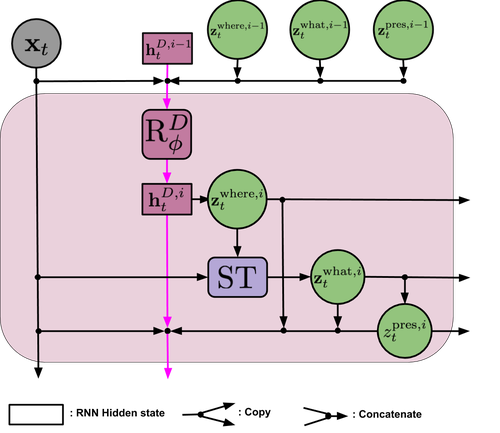
\includegraphics[width=\linewidth]{figures/SQAIR/diagrams/disc}
    \end{minipage}
    \hfill
    \begin{minipage}[c]{0.55\linewidth}
        \centering
        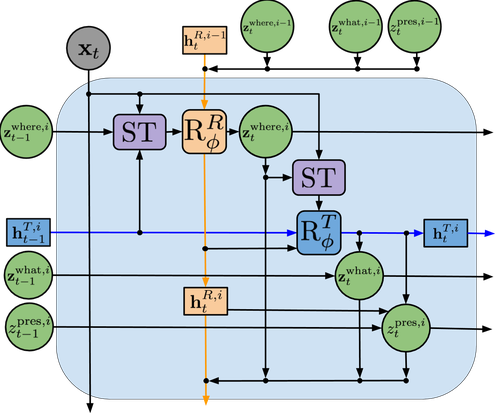
\includegraphics[width=\linewidth]{figures/SQAIR/diagrams/prop}
    \end{minipage}
\end{figure}

\textbf{Inference}
Similarly to \gls{AIR}, inference in \gls{SQAIR} can capture the number of objects and the representation describing the location and appearance of each object that is necessary to explain every image in a sequence.
As with generation, inference is divided into \gls{prop} and \gls{disc}.
During \gls{prop}, the inference network achieves two tasks.
Firstly,
the latent variables from the previous time step are used to infer the current ones, modelling the change in location and appearance of the corresponding objects, thereby attaining temporal consistency. 
This is implemented by the \textit{temporal} \gls{RNN} $\RT$, with hidden states $\textcolor{blue}{\bm{h}_t^T}$ (recurs in $t$). 
Crucially, it does not access the current image directly, but uses the output of the \textit{relation} \gls{RNN} (\textit{cf}. \cite{Santoro2017}).
The relation \gls{RNN} takes relations between objects into account, thereby implementing the \textit{explaining away} phenomenon; 
it is essential for capturing any interactions between objects as well as occlusion (or overlap, if one object is occluded by another). See \Cref{fig:partial_glimpse} for an example.  
These two \gls{RNN}s together decide whether to retain or to forget objects that have been propagated from the previous time step. 
During \gls{disc}, the network infers further latent variables that are needed to describe any new objects that have entered the frame. 
All latent variables remaining after \gls{prop} and \gls{disc} are passed on to the next time step.

See \Cref{fig:sqair_inf_flow,fig:sqair_inf_detail} for the inference network structure .
The full variational posterior is defined as
\vspace{-5pt}
\begin{equation} \label{eq:full_q}
    \q{\Dts, \bzTs}{\bxTs}{\phi} 
        = \prod_{t=1}^T \qd{ \Dt, \bzt^{\mathcal{D}_t} }{ \bxt, \bzt^{\mathcal{P}_t} }{ \phi }
        \prod_{i \in \mathcal{O}_{t-1}} \qp{\bzt^i}{\bz_{t-1}^{i}, \hT{t}{i}, \hR{t}{i}}{\phi}.
\end{equation}
Discovery, described by $\qd_\phi$, is very similar to the full posterior of \gls{AIR}, \textit{cf}. \Cref{eq:air_posterior}.
The only difference is the conditioning on $\bzt^{\mathcal{P}_t}$, which allows for a different number of discovered objects at each time-step and also for objects explained by \gls{prop} not to be explained again.
The second term, or $\qp_\phi$, describes propagation. The detailed structures of $\qd_\phi$ and $\qp_\phi$ are shown in \Cref{fig:sqair_inf_detail}, while all the pertinent algorithms and equations can be found in \Cref{app:algo,apd:sqair_inference}, respectively.

\textbf{Learning}
We train \gls{SQAIR} as an \gls{IWAE} of \cite{Burda2016iwae}. Specifically, we maximise the importance-weighted evidence lower-bound $\loss[\textsc{IWAE}]$, namely

\begin{equation} \label{eq:iwae}
\begin{aligned}
    \loss[\textsc{IWAE}] = \expc[\bxTs \sim \p{\bxTs}{}{\mathrm{data}}]{ 
        \expc[\q]{
            \log \frac{1}{K} \sum_{k=1}^K \frac{ \p{\bxTs, \bzTs}{}{\theta} }{ \q{\bzTs}{\bxTs}{\phi} }   
        }
    }.
\end{aligned}
\end{equation}
To optimise the above, we use \gls{RMSprop}, $K=5$ and batch size of $32$. We use the \textsc{vimco} gradient estimator of \cite{Mnih2016} to backpropagate through the discrete latent variables $z^{\mathrm{pres}}$, and use reparameterisation for the continuous ones \citep{Kingma2014auto}.
We also tried to use \textsc{nvil} of \cite{Mnih2014} as in the original work on \gls{AIR}, but found it very sensitive to hyper-parameters, fragile and generally under-performing.
\section{Experiments}
\label{sec:sqair_experiments}

We evaluate \gls{SQAIR} on two datasets.
Firstly, we perform an extensive evaluation on moving \gls{MNIST} digits, where we show that it can learn to reliably detect, track and generate moving digits (\Cref{sec:expr_mnist}). Moreover, we show that \gls{SQAIR} can simulate moving objects into the future --- an outcome it has not been trained for. 
We also study the utility of learned representations for a downstream task.
Secondly, we apply \gls{SQAIR} to real-world pedestrian CCTV data from static cameras (\textit{DukeMTMC}, \cite{Ristani2016performance}), where we perform background subtraction as pre-processing. In this experiment, we show that \gls{SQAIR} learns to detect, track, predict and generate walking pedestrians without human supervision.

\subsection{Moving multi-\textsc{mnist}}
\label{sec:expr_mnist}

\begin{figure}
    \centering
    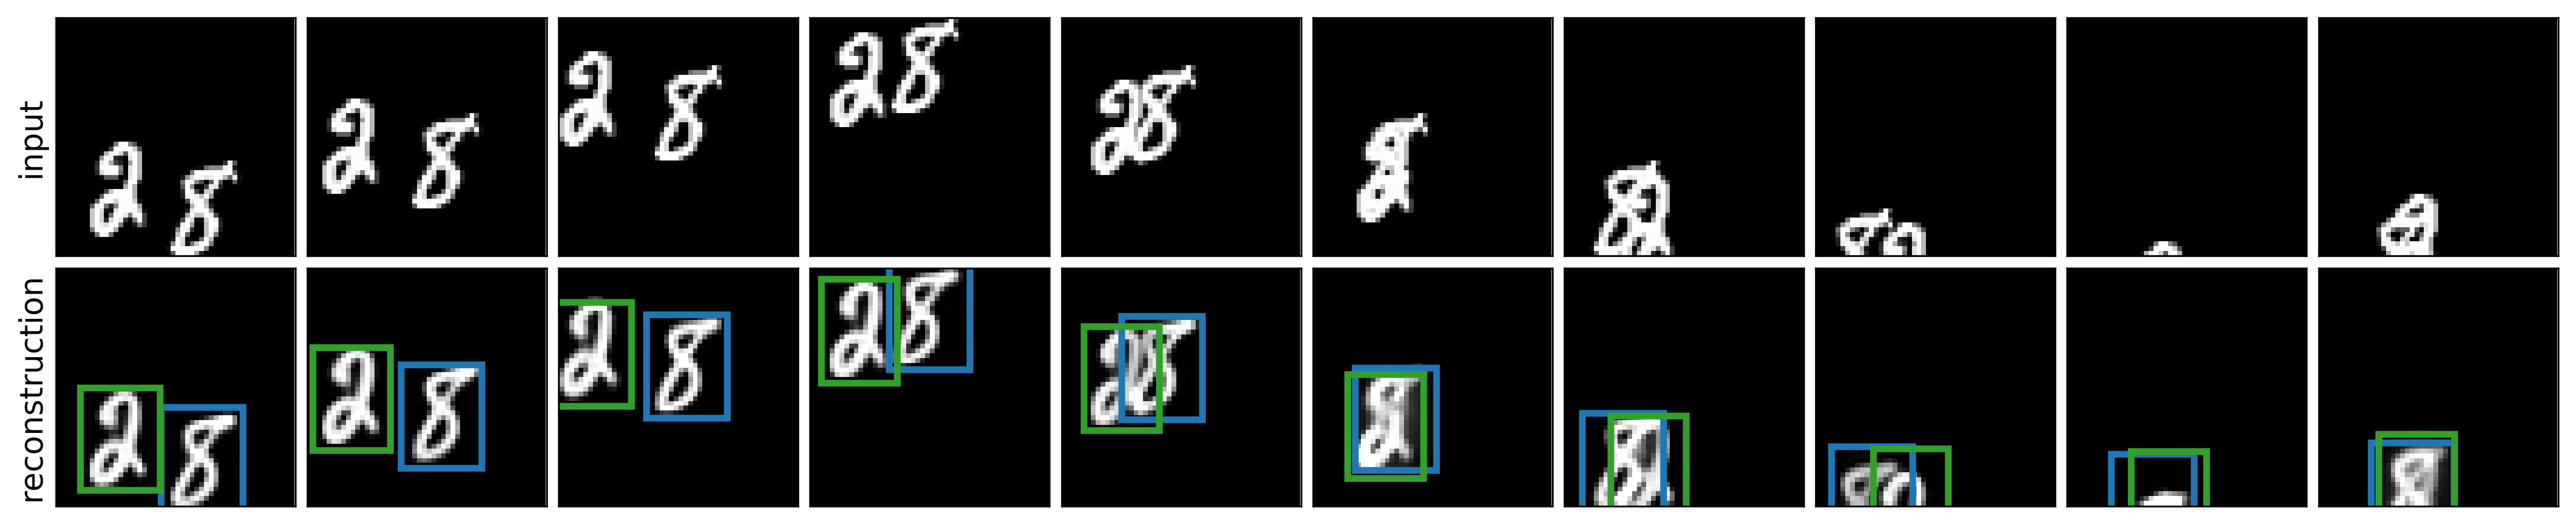
\includegraphics[width=\linewidth]{figures/SQAIR/mnist_rec/000106}
    \caption{Input images (top) and \gls{SQAIR} reconstructions with marked glimpse locations (bottom). For more examples, see \Cref{fig:mnist_recs_additional} in \Cref{app:mnist_visual}.}
    \label{fig:mnist_recs}
\end{figure}

\begin{figure}
    \centering
    
\includegraphics[width=\linewidth]{figures/SQAIR/mnist_samples/000102}
    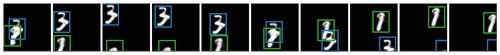
\includegraphics[width=\linewidth]{figures/SQAIR/mnist_samples/000078}
    \caption{Samples from \gls{SQAIR}. Both motion and appearance are consistent through time, thanks to the propagation part of the model. For more examples, see \Cref{fig:mnist_samples_additional} in \Cref{app:mnist_visual}.}
    \label{fig:mnist_samples}
\end{figure}
\begin{figure}
    \centering
    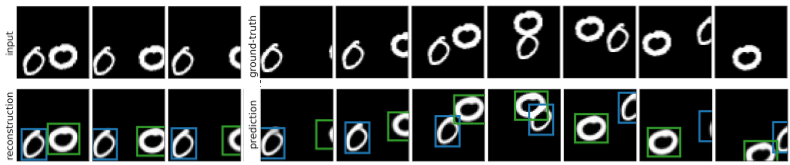
\includegraphics[width=\linewidth]{figures/SQAIR/sqair_mnist_conditional_after_three}
    \caption{The first three frames are input to \gls{SQAIR}, which generated  the rest conditional on the first frames.}
    \label{fig:mnist_cond_gen}
\end{figure}

\begin{figure}
    \centering
    \begin{minipage}[c]{0.3\linewidth}
        \centering
        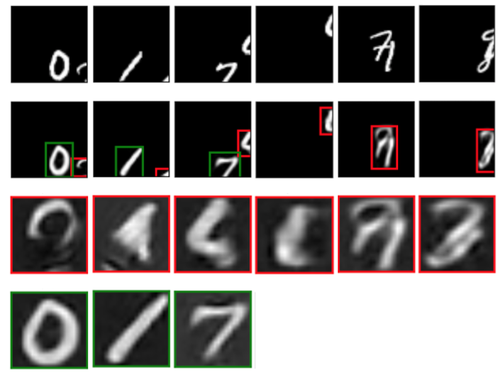
\includegraphics[width=\linewidth]{figures/SQAIR/air_partial_glimpse}
    \end{minipage}
    \hfill
    \begin{minipage}[c]{0.3\linewidth}
        \centering
        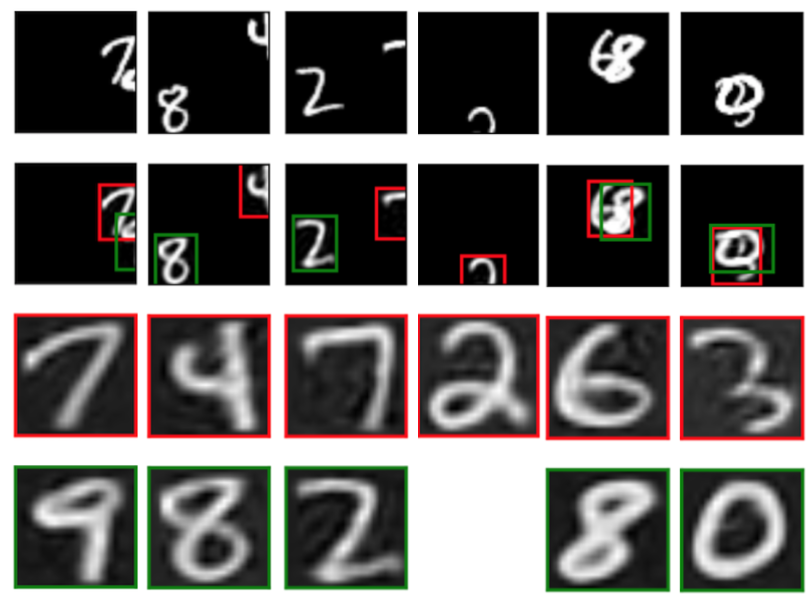
\includegraphics[width=\linewidth]{figures/SQAIR/sqair_partial_glimpse}
    \end{minipage}
       \hfill
    \begin{minipage}[c]{0.35\linewidth}
        \centering
        \caption{Inputs, reconstructions with marked glimpse locations and reconstructed glimpses for \gls{AIR} (left) and \gls{SQAIR} (right). \Gls{SQAIR} can model partially visible and heavily overlapping objects by aggregating temporal information.}
        \label{fig:partial_glimpse}
    \end{minipage}
\end{figure}


The dataset consists of sequences of length 10 of multiple moving \gls{MNIST} digits. All images are of size $50 \times 50$ and there are zero, one or two digits in every frame (with equal probability).
Sequences are generated such that no objects overlap in the first frame, and all objects are present through the sequence; the digits can move out of the frame, but always come back.
See \Cref{app:mnist_inout} for an experiment on a harder version of this dataset.
There are 60,000 training and 10,000 testing sequences created from the respective \gls{MNIST} datasets.
We train two variants of \gls{SQAIR}: the \textsc{mlp}-\gls{SQAIR} uses only fully-connected networks, while the \textsc{conv}-\gls{SQAIR} replaces the networks used to encode images and glimpses with convolutional ones; it also uses a subpixel-convolution network as the glimpse decoder \citep{Shi2016subpixel}.
See \Cref{app:mnist_details} for details of the model architectures and the training procedure.

We use \gls{AIR} and \gls{VRNN} \citep{Chung2015} as baselines for comparison.  \gls{VRNN} can be thought of as a sequential \gls{VAE} with an \gls{RNN} as its deterministic backbone. Being similar to a \gls{VAE}, its latent variables are not structured, nor easily interpretable. For a fair comparison, we control the latent dimensionality of $\gls{VRNN}$ and the number of learnable parameters. We provide implementation details in \Cref{apd:vrnn}.

\begin{table}
    \centering
    \begin{tabular}{c|c|c|c|c|c}
                         & $\log \p{\bxTs}{}{\theta}$ & $\log \p{\bxTs}{\bzTs}{\theta}$  & $\kl{\q{}{}{\phi}}{\p{}{}{\theta}}$ & Counting & Addition\\
                         \hline
        \textsc{conv}-\gls{SQAIR} & $\bm{6784.8}$ & $\bm{6923.8}$ & $\bm{134.6}$ & $0.9974$ & $0.9990$ \\
        \textsc{mlp}-\gls{SQAIR}  & $6617.6$      & $6786.5$      & $164.5$      & $\mathbf{0.9986}$ & $\mathbf{0.9998}$ \\
        \textsc{mlp}-\gls{AIR}    & $6443.6$      & $6830.6$      & $352.6$      & $0.9058$ & $0.8644$\\
        \textsc{conv}-\gls{VRNN}  & $6561.9$      & $6737.8$      & $270.2$      & n/a & $0.8536$\\
        \textsc{mlp}-\gls{VRNN}   & $5959.3$      & $6108.7$      & $218.3$      & n/a  & 0.8059 \\
    \end{tabular}
    \vspace{5pt}
    \caption{\gls{SQAIR} achieves higher performance than the baselines across a range of metrics. The third column refers to the \gls{KL} divergence between the approximate posterior and the prior. Counting refers to accuracy of the inferred number of objects present in the scene, while addition stands for the accuracy of a supervised digit addition experiment, where a classifier is trained on the learned latent representations of each frame.}
    \label{tab:quant}
    %\vspace{-15pt}
\end{table}

The quantitative analysis consists of comparing all models in terms of the marginal log-likelihood $\log \p{\bxTs}{}{\theta}$ evaluated as the $\loss[\textsc{IWAE}]$ bound with $K=1000$ particles, reconstruction quality evaluated as a single-sample approximation of $\expc[\q{}{}{\phi}]{\log \p{\bxTs}{\bzTs}{\theta}}$ and the \gls{KL}-divergence between the approximate posterior and the prior (\Cref{tab:quant}). Additionally, we measure the accuracy of the number of objects modelled by \gls{SQAIR} and \gls{AIR}. \Gls{SQAIR} achieves superior performance across a range of metrics --- its convolutional variant outperforms both \gls{AIR} and the corresponding \gls{VRNN} in terms of model evidence and reconstruction performance. 
% 
The \gls{KL} divergence for \gls{SQAIR} is almost twice as low as for \gls{VRNN} and by a yet larger factor for \gls{AIR}.
We can interpret \gls{KL} values as an indicator of the ability to compress, and we can treat \gls{SQAIR}/\gls{AIR} type of scheme as a version of run-length encoding.
While \gls{VRNN} has to use information to explicitly describe every part of the image, even if some parts are empty, \gls{SQAIR} can explicitly allocate content information ($\bz^\mathrm{what}$) to specific parts of the image (indicated by $\bz^\mathrm{where}$).
\Gls{AIR} exhibits the highest values of \gls{KL}, but this is due to encoding every frame of the sequence independently --- its prior cannot take \textit{what} and \textit{where} at the previous time-step into account, hence higher KL.
% 
The fifth column of \Cref{tab:quant} details the object counting accuracy, that is indicative of the quality of the approximate posterior. It is measured as the sum of $\zt^\mathrm{pres}$ for a given frame against the true number of objects in that frame. As there is no $z^\mathrm{pres}$ for \gls{VRNN} no score is provided. Perhaps surprisingly, this metric is much higher for \gls{SQAIR} than for \gls{AIR}. This is because \gls{AIR} mistakenly infers overlapping objects as a single object. Since \gls{SQAIR} can incorporate temporal information, it does not exhibit this failure mode (\textit{cf}. \Cref{fig:partial_glimpse}).
Next, we gauge the utility of the learnt representations by using them to determine the sum of the digits present in the image (\Cref{tab:quant}, column six). To do so, we train a 19-way classifier (mapping from any combination of up to two digits in the range $[0, 9]$ to their sum) on the extracted representations and use the summed labels of digits present in the frame as the target. \Cref{app:mnist_details} contains details of the experiment. 
\Gls{SQAIR} significantly outperforms \gls{AIR} and both variants of \gls{VRNN} on this tasks.
\Gls{VRNN} under-performs due to the inability of disentangling overlapping objects, while both \gls{VRNN} and \gls{AIR} suffer from low temporal consistency of learned representations, see \Cref{app:mnist_visual}. 
Finally, we evaluate \gls{SQAIR} qualitatively by analyzing reconstructions and samples produced by the model against reconstructions and samples from \gls{VRNN}.
We observe that samples and reconstructions from \gls{SQAIR} are of better quality and, unlike \gls{VRNN}, preserve motion and appearance consistently through time. See \Cref{app:mnist_visual} for direct comparison and additional examples.
Furthermore, we examine conditional generation, where we look at samples from the generative model of \gls{SQAIR} conditioned on three images from a real sequence (see \Cref{fig:mnist_cond_gen}).
We see that the model can preserve appearance over time, and that the simulated objects follow similar trajectories, which hints at good learning of the motion model (see \Cref{app:mnist_visual} for more examples).
\Cref{fig:partial_glimpse} shows reconstructions and corresponding glimpses of \gls{AIR} and \gls{SQAIR}. Unlike \gls{SQAIR}, \gls{AIR} is unable to recognize objects from partial observations, nor can it distinguish strongly overlapping objects (it treats them as a single object; columns five and six in the figure).
We analyze failure cases of \gls{SQAIR} in \Cref{app:fail}.

% ## 10 timesteps, 3 objects
% # conv-sqair 500k
% # {'data_ll': 199.5723372428648,
% #  'iwae': 1338.4910140498991,
% #  'kl': 65.56289869739163,
% #  'log_p_z': 47.66771562637821,
% #  'log_q_z_given_x': 113.23061346238659,
% #  'steps': 2.366231826043898,
% #  'steps_acc': 0.3843745406596891,
% #  'vae': 556.3954507150958}
% 
% # mlp-sqair 900k
% {'data_ll': 345.1663582094254,
%  'iwae': 2829.1831290952623,
%  'kl': 62.08844412526777,
%  'log_p_z': 2.4096233662097686,
%  'log_q_z_given_x': 64.49806619459584,
%  'steps': 2.1725647372584187,
%  'steps_acc': 0.2108948781125007,
%  'vae': 2377.875941122732}
% 
% ## digit adding
% mlp-sqair 0.09997
% mlp-air   0.8609
% conv-vrnn 0.8419
% 
% ## 10 timesteps, {0, 1, 2} objects
% # iwae-5
% conv-sqair 6719.108
% mlp-sqair 6607.305
% mlp-air   6385
% 
% # iwae-1000
% conv-sqair 6778.93453369
% mlp-sqair 6541.71697559
% mlp-air 6443.57998547
% 
% # num step acc
% conv-sqair 0.9974
% mlp-sqair  0.9846 
% mlp-air    0.9058 0.905345526785
% 
% # rec
% conv-sqair 6919.84491394
% mlp-sqair  6741.62037109
% mlp-air    6830.56475928
% 
% # kl
% conv-sqair 136.518626827
% mlp-sqair  195.4172697
% mlp-air    352.594786018


\subsection{Generative Modelling of Walking Pedestrians}
\label{sec:expr_duke}

\begin{figure}
    \centering
    \begin{minipage}[c]{0.49\linewidth}
        \centering
        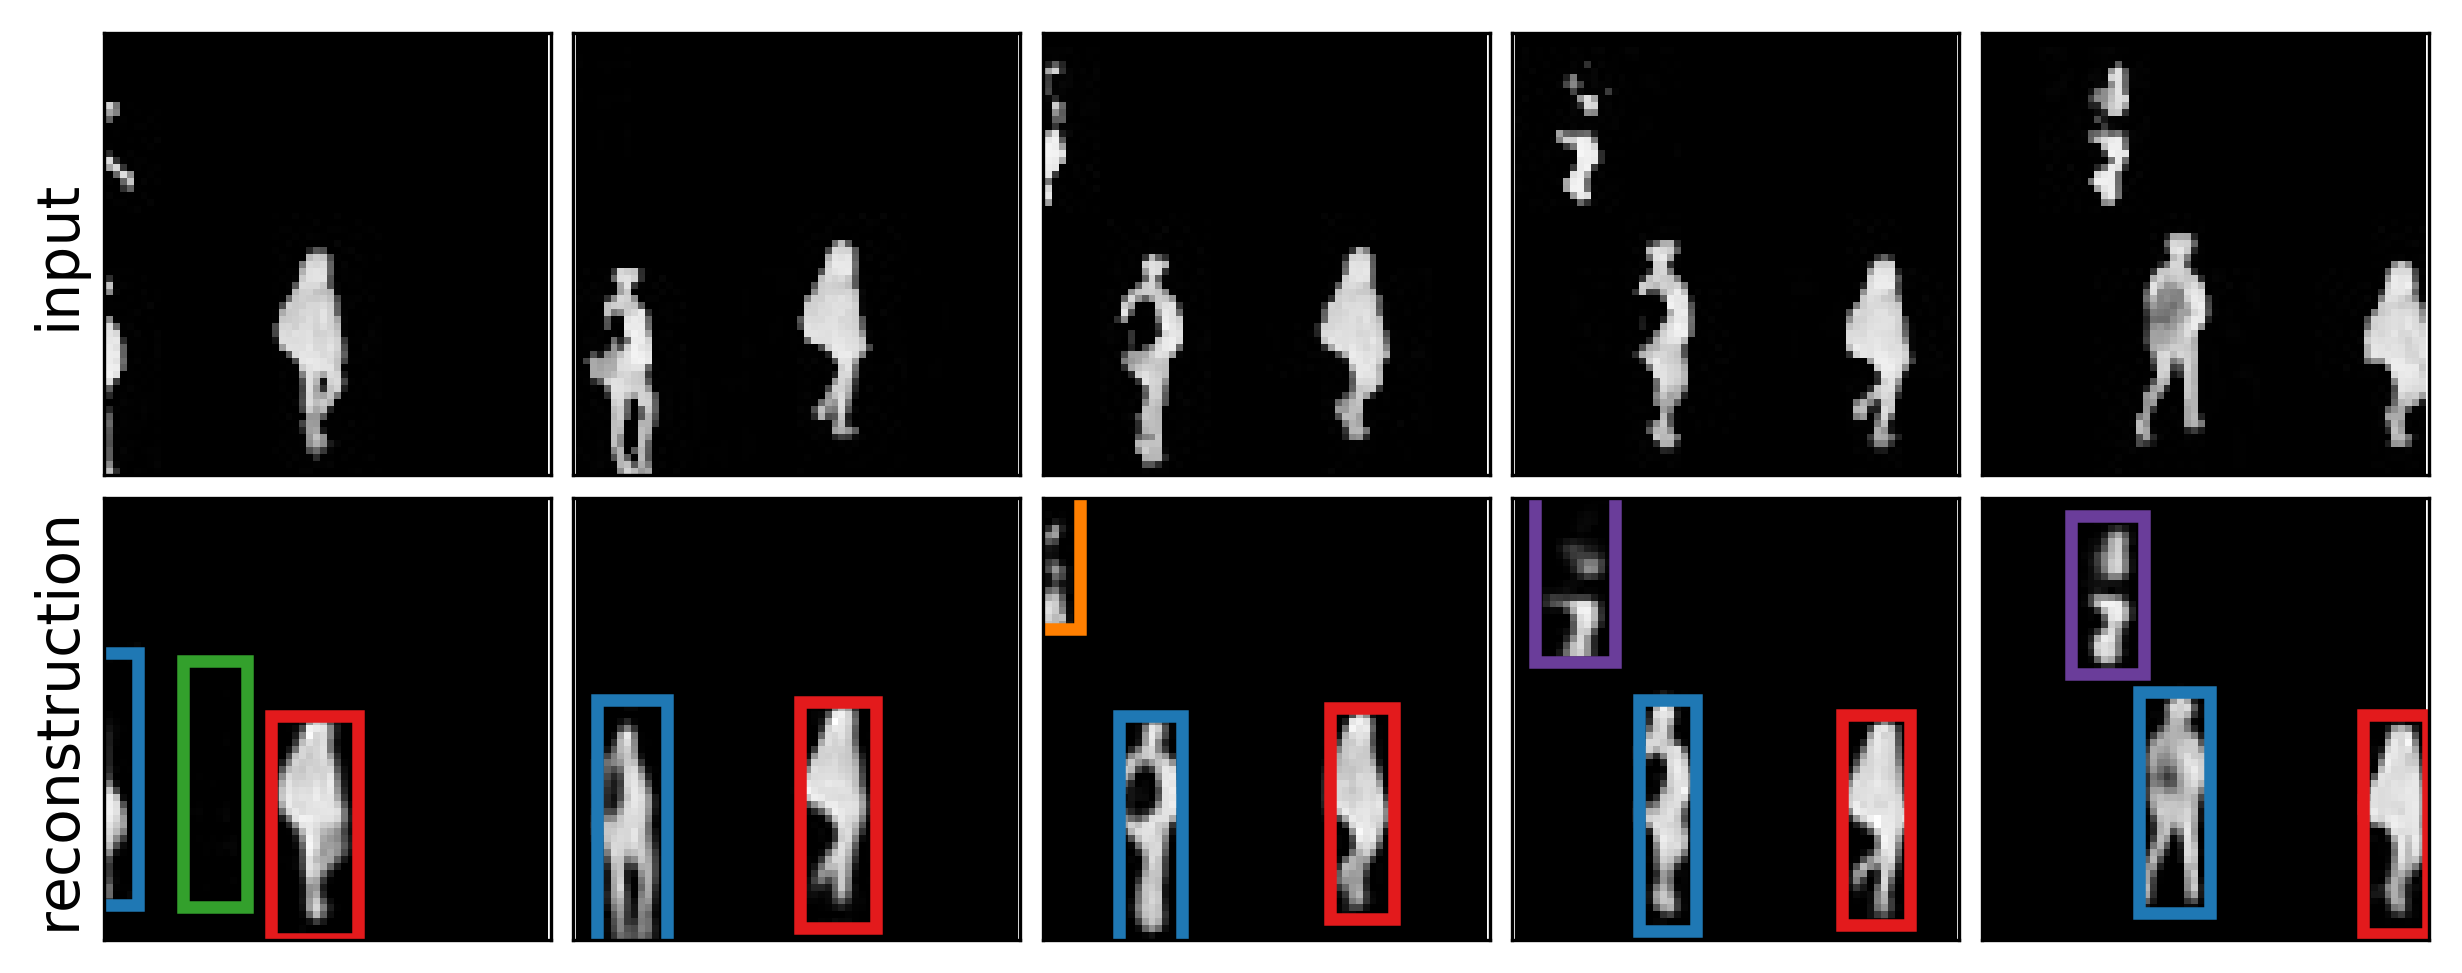
\includegraphics[width=\linewidth]{figures/SQAIR/duke_rec/front/000065}
        % 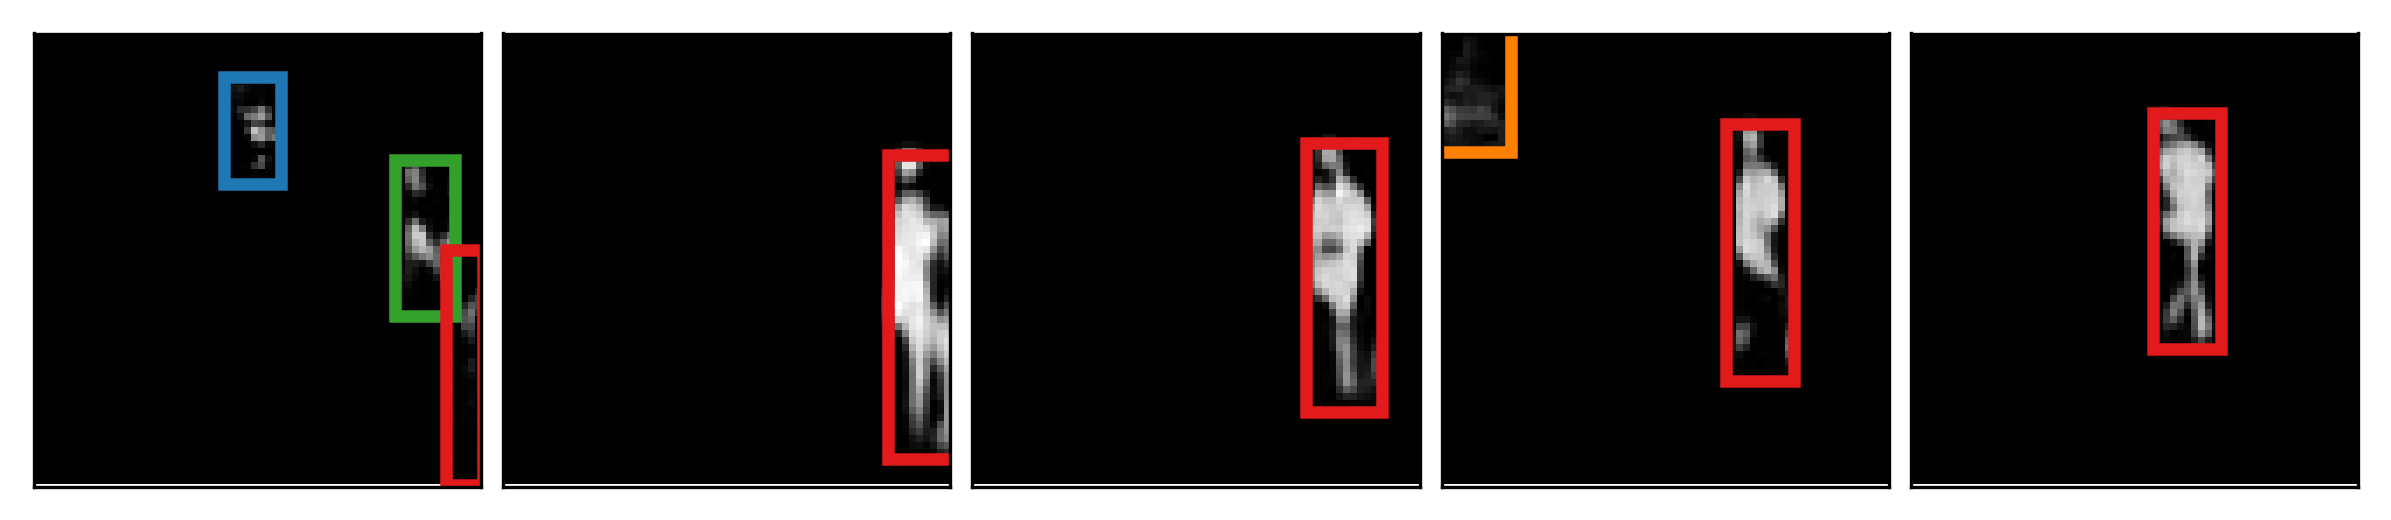
\includegraphics[width=\linewidth]{figures/SQAIR/duke_sample/front/000296}
        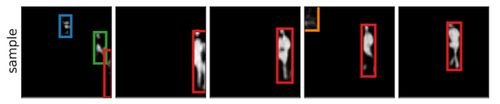
\includegraphics[width=\linewidth]{figures/SQAIR/duke_sample/front/sqair_duke_sample_with_label_296}
    \end{minipage}
    \hfill
    \begin{minipage}[c]{0.49\linewidth}
        \centering
        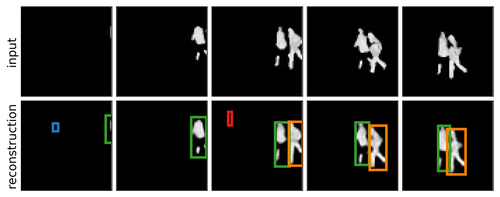
\includegraphics[width=\linewidth]{figures/SQAIR/duke_rec/front/000099}
        % 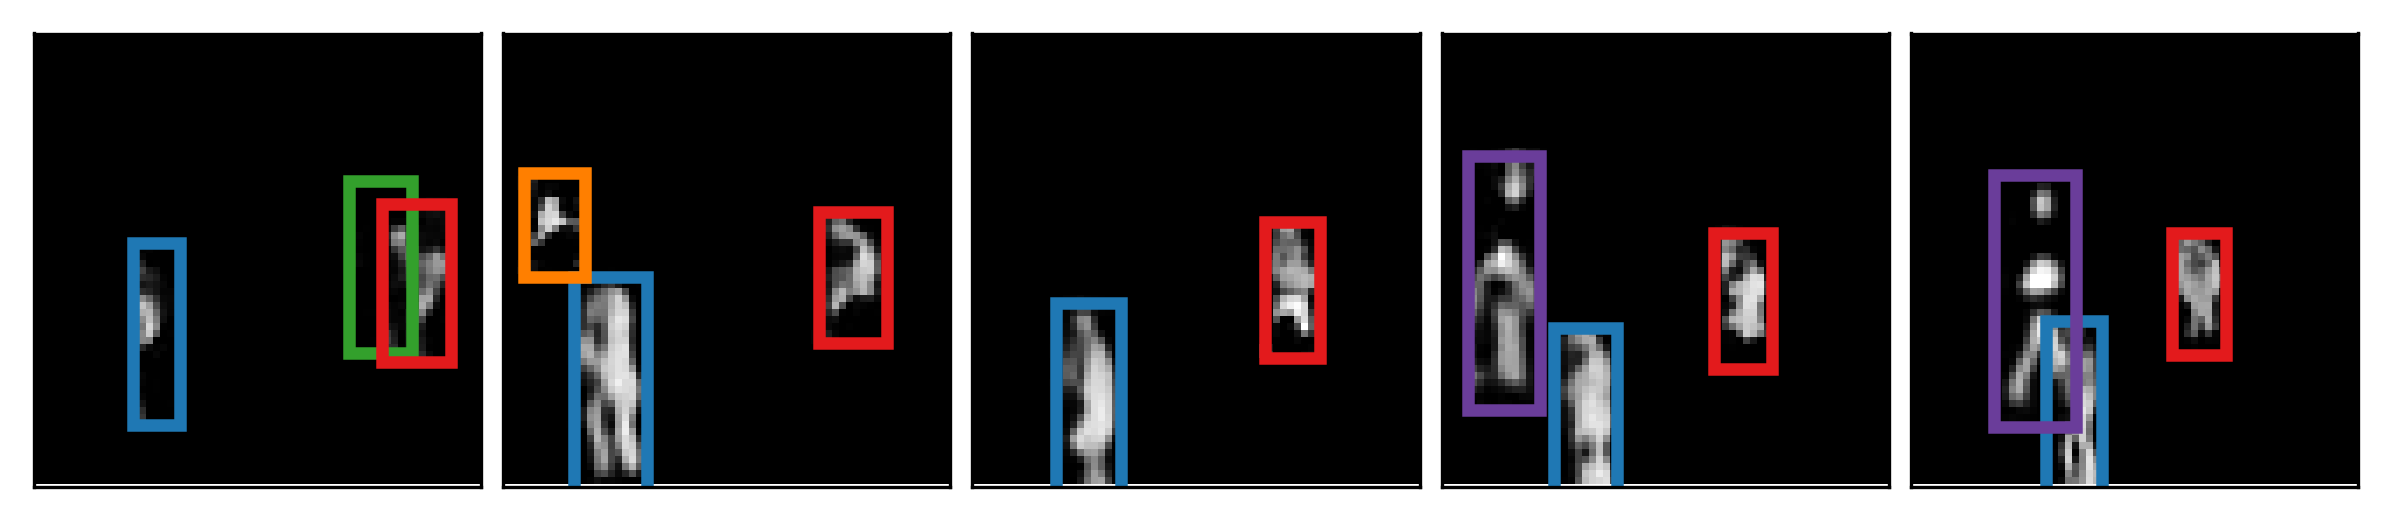
\includegraphics[width=\linewidth]{figures/SQAIR/duke_sample/front/000020}
       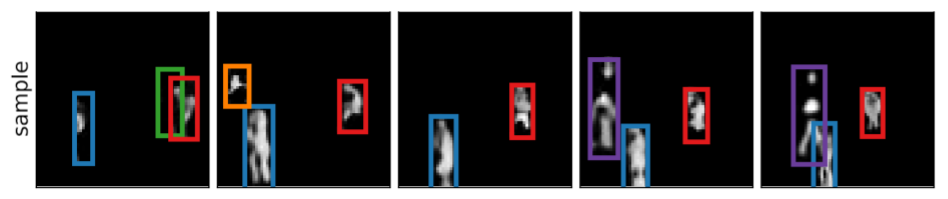
\includegraphics[width=\linewidth]{figures/SQAIR/duke_sample/front/sqair_duke_sample_with_label_020}
    \end{minipage}
    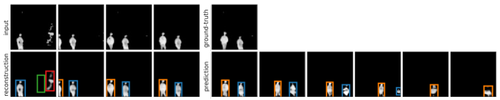
\includegraphics[width=.95\linewidth]{figures/SQAIR/duke_cond_gen/front/sqair_duke_cond_after_four}
    \caption{Inputs on the top, reconstructions in the second row, samples in the third row; rows four and five contain inputs and conditional generation: the first four frames in the last row are reconstructions, while the remaining ones are predicted by sampling from the prior. There is no ground-truth, since we used sequences of length five of training and validation.}
    \label{fig:duke_rec}
\end{figure}
To evaluate the model in a more challenging, real-world setting, we turn to data from static CCTV cameras of the \textit{DukeMTMC} dataset \citep{Ristani2016performance}. As part of pre-precessing, we use standard background subtraction algorithms \citep{Itseez2015opencv}. In this experiment, we use $3150$ training and $350$ validation sequences of length $5$. For details of model architectures, training and data pre-processing, see \Cref{app:duke_details}.
We evaluate the model qualitatively by examining reconstructions, conditional samples (conditioned on the first four frames) and samples from the prior (\Cref{fig:duke_rec} and \Cref{app:duke_visual}).
We see that the model learns to reliably detect and track walking pedestrians, even when they are close to each other.

There are some spurious detections and re-detections of the same objects, which is mostly caused by imperfections of the background subtraction pipeline --- backgrounds are often noisy and there are sudden appearance changes when a part of a person is treated as background in the pre-processing pipeline.
The object counting accuracy in this experiment is $0.5712$ on the validation dataset, and we noticed that it does increase with the size of the training set. We also had to use early stopping to prevent overfitting, and the model was trained for only $315$k iterations ($>1$M for \textsc{mnist} experiments). Hence, we conjecture that accuracy and marginal likelihood can be further improved by using a bigger dataset.
\section{Related Work}

\begin{description}[leftmargin=\parindent]
\item[Object Tracking]
    There have been many approaches to modelling objects in images and videos. 
    Object detection and tracking are typically learned in a supervised manner, where object bounding boxes and often additional labels are part of the training data.
    Single-object tracking commonly use Siamese networks, which can be seen as an \gls{RNN} unrolled over two time-steps \citep{valmadre2017end}. Recently, \cite{kosiorek2017hierch} used an \gls{RNN} with an attention mechanism in the \textsc{hart} model to predict bounding boxes for single objects, while robustly modelling their motion and appearance. Multi-object tracking is typically attained by detecting objects and performing data association on bounding-boxes \citep{bewley2016sort}.
    \cite{schulter2017deepnf} used an end-to-end supervised approach that detects objects and performs data association.
    In the unsupervised setting, where the training data consists of only images or videos, the dominant approach is to distill the inductive bias of spatial consistency into a discriminative model.  \cite{cho2015unsupervised} detect single objects and their parts in images, and \cite{kwak2015unsupervised,xiao2016track} incorporate temporal consistency to better track single objects.
    \Gls{SQAIR} is unsupervised and hence it does not rely on bounding boxes nor additional labels for training, while being able to learn arbitrary motion and appearance models similarly to \textsc{hart} \citep{kosiorek2017hierch}.
    At the same time, is inherently multi-object and performs data association implicitly (\textit{cf}. \Cref{app:algo}).
    Unlike the other unsupervised approaches, temporal consistency is baked into the model structure of \gls{SQAIR} and further enforced by lower \gls{KL} divergence when an object is tracked.

\item[Video Prediction]
     Many works on video prediction learn a deterministic model conditioned on the current frame to predict the future ones \citep{ranzato2014video,srivastava2015unsupervised}.
     Since these models do not model uncertainty in the prediction, they can suffer from the multiple futures problem --- since perfect prediction is impossible, the model produces blurry predictions which are a mean of possible outcomes.
     This is addressed in stochastic latent variable models trained using variational inference to generate multiple plausible videos given a sequence of images \citep{babaeizadeh2017stochastic, denton2018stochastic}.
     Unlike \gls{SQAIR}, these approaches do not model objects or their positions explicitly, thus the representations they learn are of limited interpretability. 
     
\item[Learning Decomposed Representations of Images and Videos]
    Learning decomposed representations of object appearance and position lies at the heart of our model.
    This problem can be also seen as perceptual grouping, which involves modelling pixels as spatial mixtures of entities.
    \cite{Greff2016tagger} and \cite{Greff2017neuralem} learn to decompose images into separate entities by iterative refinement of spatial clusters using either learned updates or the Expectation Maximization algorithm;
    \cite{Ilin2017recurrentln} and \cite{Steenkiste2018relationalnem} extend these approaches to videos, achieving very similar results to \gls{SQAIR}.
    Perhaps the most similar work to ours is the concurrently developed model of \cite{Hsieh2018ddpae}.
    The above approaches rely on iterative inference procedures, but do not exhibit the object-counting behaviour of \gls{SQAIR}.
    For this reason, their computational complexities are proportional to the predefined maximum number of objects, while \gls{SQAIR} can be more computationally efficient by adapting to the number of objects currently present in an image.
    
    Another interesting line of work is the \textsc{gan}-based unsupervised video generation that decomposes motion and content \citep{tulyakov2017mocogan,denton2017unsupervised}. These methods learn interpretable features of content and motion, but deal only with single objects and do not explicitly model their locations. Nonetheless, adversarial approaches to learning structured probabilistic models of objects offer a plausible alternative direction of research.
    
\item[Bayesian Nonparametric Models]
    To the best of our knowledge, \cite{neiswanger2012unsupervised} is the only known approach that models pixels belonging to a variable number of objects in a video together with their locations in the generative sense.
    This work uses a \gls{bnp} model, which relies on mixtures of Dirichlet processes to cluster pixels belonging to an object. 
    However, the choice of the model necessitates complex inference algorithms involving Gibbs sampling and Sequential Monte Carlo, to the extent that any sensible approximation of the marginal likelihood is infeasible.
    It also uses a fixed likelihood function, while ours is learnable.
    
    The object appearance-persistence-disappearance model in \gls{SQAIR} is reminiscent of the \gls{mibp} of \cite{Gael2009}, another \gls{bnp} model. \Gls{mibp} was used as a model for blind source separation, where multiple sources contribute toward an audio signal, and can appear, persist, disappear and reappear independently. 
    The prior in \gls{SQAIR} is similar, but the crucial differences are that \gls{SQAIR} combines the \gls{bnp} prior with flexible neural network models for the dynamics and likelihood, as well as variational learning via amortized inference.
    The interface between deep learning and \gls{bnp}, and graphical models in general, remains a fertile area of research.
\end{description}
\section{Discussion}
\label{sec:discussion}

In this paper we proposed \gls{SQAIR}, a probabilistic model that extends \gls{AIR} to image sequences, and thereby achieves temporally consistent reconstructions and samples. In doing so, we enhanced \gls{AIR}'s capability of disentangling overlapping objects and identifying partially observed objects.

This work continues the thread of
\cite{Greff2017neuralem}, \cite{Steenkiste2018relationalnem} and, together with \cite{Hsieh2018ddpae}, presents unsupervised object detection~\&~tracking with learnable likelihoods by the means of generative modelling of objects.
In particular, our work is the first one to explicitly model object presence, appearance and location through time. 
Being a generative model, \gls{SQAIR} can be used for conditional generation, where it can extrapolate sequences into the future.
As such, it would be interesting to use it in a reinforcement learning setting in conjunction with Imagination-Augmented Agents \citep{Weber2017imagination} or more generally as a world model \citep{Ha2018worldm}, especially for settings with simple backgrounds,\eg games like Montezuma's Revenge or Pacman.

The framework offers various avenues of further research; 
\Gls{SQAIR} leads to interpretable representations, but the interpretability of \textit{what} variables can be further enhanced by using alternative objectives that disentangle factors of variation in the objects \citep{Kim2018disentangling}. 
Moreover, in its current state, \gls{SQAIR} can work only with simple backgrounds and static cameras. In future work, we would like to address this shortcoming, as well as speed up the sequential inference process whose complexity is linear in the number of objects. The generative model, which currently assumes additive image composition, can be further improved by\eg autoregressive modelling \citep{Oord2016cond}. It can lead to higher fidelity of the model and improved handling of occluded objects. Finally, the \gls{SQAIR} model is very complex, and it would be useful to perform a series of ablation studies to further investigate the roles of different components.
\section*{Acknowledgements}

We would like to thank Ali Eslami for his help in implementing \gls{AIR}, Alex Bewley and Martin Engelcke for discussions and valuable insights and anonymous reviewers for their constructive feedback. Additionally, we acknowledge that HK and YWT's research leading to these results has received funding from the European Research Council under the European Union's Seventh Framework Programme (FP7/2007-2013) ERC grant agreement no. 617071.



\begin{subappendices}
	\section{Algorithms}
\label{app:algo}

Image generation, described by \Cref{algo:air_decoding}, is exactly the same for \gls{SQAIR} and \gls{AIR}.
\Cref{algo:sqair_prop,algo:sqair_disc} describe inference in \gls{SQAIR}. Note that \gls{disc} is equivalent to \gls{AIR} if no latent variables are present in the inputs.

If a function has multiple inputs and if not stated otherwise, all the inputs are concatenated and linearly projected into some fixed-dimensional space,\eg\Cref{l:rel_rnn,l:q_pres} in \Cref{algo:sqair_prop}.
Spatial Transformer ($\STN$,\eg \Cref{l:prop_glimpse} in \Cref{algo:sqair_prop}) has no learnable parameters: it samples a uniform grid of points from an image $\bx$, where the grid is transformed according to parameters $\bz^\mathrm{where}$.
$\operatorname{f_\phi^1}$~is implemented as a perceptron with a single hidden layer.
Statistics of $\qp$ and $\qd$ are a result of applying a two-layer \gls{MLP} to their respective conditioning sets.
Different distributions $\q$ do not share parameters of their \glspl{MLP}.
The \textit{glimpse encoder} $\operatorname{h_\phi^\mathrm{glimpse}}$ (\Cref{l:glimpse_enc_prop,l:glimpse_enc_final} in \Cref{algo:sqair_prop} and \Cref{l:glimpse_enc_disc} in \Cref{algo:sqair_disc}; they share parameters) and the \textit{image encoder} $\operatorname{h_\phi^\mathrm{enc}}$ (\Cref{l:img_encoder} in \Cref{algo:sqair_disc}) are implemented as two-layer \glspl{MLP} or \glspl{CNN}, depending on the experiment (see \Cref{app:mnist_details,app:duke_details} for details).

One of the important details of \gls{prop} is the proposal glimpse extracted in lines \Cref{l:prop_where,l:prop_glimpse} of \Cref{algo:sqair_prop}. 
It has a dual purpose. 
Firstly, it acts as an information bottleneck in \gls{prop}, limiting the flow of information from the current observation $\bxt$ to the updated latent variables $\bzt$.
Secondly, even though the information is limited, it can still provide a high-resolution view of the object corresponding to the currently updated latent variable, \textit{given} that the location of the proposal glimpse correctly predicts motion of this object.
Initially, our implementation used encoding of the raw observation ($\operatorname{h_\phi^\mathrm{enc}} \left( \bxt \right)$, similarly to \Cref{l:img_encoder} in \Cref{algo:sqair_disc}) as an input to the relation-\gls{RNN} (\Cref{l:rel_rnn} in \Cref{algo:sqair_prop}). We have also experimented with other bottlenecks: (1) low resolution image as an input to the image encoder and (2) a low-dimensional projection of the image encoding before the relation-\gls{RNN}. 
Both approaches have led to \textit{ID swaps}, where the order of explaining objects were sometimes swapped for different frames of the sequence (see \Cref{fig:id_swap} in \Cref{app:fail} for an example). 
Using encoded proposal glimpse extracted from a predicted location has solved this issue.
% \ak{should we create a "discussion" appendix and move this paragraph there?}

To condition \gls{disc} on propagated latent variables (\Cref{l:latent_enc} in \Cref{algo:sqair_disc}), we encode the latter by using a two-layer \gls{MLP} similarly to \cite{zaheer2017deeps},
\begin{equation}
    \blt = \sum_{i \in \mathcal{P}_t} \operatorname{MLP} \left( \bzt^{\mathrm{what}, i}, \bzt^{\mathrm{where}, i} \right).
\end{equation}
Note that other encoding schemes are possible, though we have experimented only with this one.

\begin{algorithm}
    \caption{Image Generation}
    \label{algo:air_decoding}
    \DontPrintSemicolon
    \SetKwInOut{Input}{Input}
    \SetKwInOut{Output}{Output}
    \SetSideCommentLeft
    \Input{
        $\bzt^\mathrm{what},
         \bzt^\mathrm{where}$ 
         - latent variables from the current time-step.\\
    }
    % 
    $\mathcal{O}_t = \operatorname{indices} \left( \bzt^\mathrm{what} \right)$ \tcp*{Indices of all present latent variables.}
    $\byt^0 = \bm{0}$\\
    \For{$i \in \mathcal{O}_t$}{
        $\byt^{\mathrm{att}, i} = \operatorname{f_\theta^\mathrm{dec}} \left( 
            \bzt^{\mathrm{what}, i} 
        \right)$ \tcp*{Decode the glimpse.}
% 
        $\byt^i = \byt^{i-1} + \STN^{-1} \left( 
            \byt^{\mathrm{att}, i}, \bzt^{\mathrm{where}, i} 
        \right)$
    }
    $\hat{\bx}_t \sim \mathcal{N} \left(\bm{x} \mid \bm{y}_n, \sigma^2_x \bm{I} \right)$\\
    \Output{$\hat{\bm{x}}$}
\end{algorithm}

\begin{algorithm}
    \caption{Inference for Propagation}
    \label{algo:sqair_prop}
    \DontPrintSemicolon
    \SetKwInOut{Input}{Input}
    \SetKwInOut{Output}{Output}
    \SetSideCommentLeft
    \Input{$\bm{x_t}$ - image at the current time-step,\\
         $\bz^\mathrm{what}_{t-1},
         \bz^\mathrm{where}_{t-1},
         \bz^\mathrm{pres}_{t-1}$ 
         - latent variables from the previous time-step\\
         $\bm{h}^T_{t-1}$ - hidden states from the previous time-step.
    }
    $\hR{t}{0}, \bm{z}^{\mathrm{what}, 0}_t, \bm{z}^{\mathrm{where}, 0}_t = \operatorname{initialize}()$\\
    $j = 0$ \tcp*{Index of the object processed in the last iteration.}
    \For{$i \in {\mathcal{O}_{t-1}}$}{
% 
        \uIf{$z_{t-1}^{\mathrm{pres}, i} == 0$}{
            \Continue
        }
%       
        $\hat{\bz}_t^{\mathrm{where}, i} = \operatorname{f_\phi^1} \left( \bz_{t-1}^{\mathrm{where}, i},
            \hT{t}{i} \right)$ \label{l:prop_where}\tcp*{Proposal location.}
% 
        $\hat{\bg}^i_t = \STN \left(
            \bxt, \hat{\bz}_t^{\mathrm{where}, i}
        \right)$ \label{l:prop_glimpse}\tcp*{Extract a glimpse from a proposal location.}
% 
    $\hat{\be}_t^i = \operatorname{h_\phi^\mathrm{glimpse}} \left( \hat{\bg}^i_t \right)$ \label{l:glimpse_enc_prop}\tcp*{Encode the proposal glimpse.}
% 
        $\textcolor{orange}{\bwt^{R, i}}, \hR{t}{i} = \Rr \left(
            \hat{\be}_t^i,
            \bz_{t-1}^{\mathrm{what}, i}, \bz_{t-1}^{\mathrm{where}, i}, 
            \hT{t-1}{i}, \hR{t}{j},
            \bzt^{\mathrm{what}, j}, \bzt^{\mathrm{where}, j}
        \right)$  
        \label{l:rel_rnn}\tcp*{Relational state, see \Cref{eq:propagation_state}.}
%         
        $\bzt^{\mathrm{where}, i} \sim \qp{\bm{z}^\mathrm{where}}{\bm{z}^{\mathrm{where}, k}_{t-1}, \textcolor{orange}{\bwt^{R, i}}}{\phi}$\\
%        
        $\bgt^i = \STN \left( 
            \bxt,
            \bzt^{\mathrm{where}, i}
        \right)$ \tcp*{Extract the final glimpse.}
    % 
    $\bet^i = \operatorname{h_\phi^\mathrm{glimpse}} \left( \bgt^i \right)$ \label{l:glimpse_enc_final}\tcp*{Encode the final glimpse.}
    % 
        $\textcolor{blue}{\bwt^{T, i}}, \hT{t}{i} = \RT \left(
            \bet^i,
            \bzt^{\mathrm{where}, i}, 
            \hT{t-1}{i}, \hR{t}{i}
        \right)$
        \label{l:time_rnn}\tcp*{Temporal state, see \Cref{eq:temporal_state}.}
%        
        $\bzt^{\mathrm{what}, i} \sim \qp {\bz^\mathrm{what}}{\bet^i, \bz_{t-1}^{\mathrm{what}, i}, \textcolor{orange}{\bwt^{R, i}}, \textcolor{blue}{\bwt^{T, i}}}{\phi}$\\
%        
        $\zt^{\mathrm{pres}, i} \sim \qp{z^\mathrm{pres}}{
            z_{t-1}^{\mathrm{pres}, i},
            \bzt^{\mathrm{what}, i},
            \bzt^{\mathrm{where}, i},
            \textcolor{orange}{\bwt^{R, i}},
            \textcolor{blue}{\bwt^{T, i}}}{\phi}$ \label{l:q_pres}\tcp*{\Cref{eq:q_prop_presence}.}
        $j = i$
    }
    \Output{
        $\bzt^{\mathrm{what}, \mathcal{P}_t},
        \bzt^{\mathrm{where}, \mathcal{P}_t},
        \bzt^{\mathrm{pres}, \mathcal{P}_t}$
    }
\end{algorithm}

\begin{algorithm}
    \caption{Inference for Discovery}
    \label{algo:sqair_disc}
    \DontPrintSemicolon
    \SetKwInOut{Input}{Input}
    \SetKwInOut{Output}{Output}
    \SetSideCommentLeft
    \Input{
        $\bm{x_t}$ - image at the current time-step,\\
        $\bzt^{\mathcal{P}_t}$ - propagated latent variables for the current time-step,\\
        $N$ - maximum number of inference steps for discovery.
    }
% 
    $\hD{t}{0}, \bm{z}^{\mathrm{what}, 0}_t, \bm{z}^{\mathrm{where}, 0}_t = \operatorname{initialize}()$\\
% 
    $j = \operatorname{max\_index} \left( \bzt^{\mathcal{P}_t} \right)$ \tcp*{Maximum index among the propagated latent variables.}
% 
    $\bet = \operatorname{h_\phi^\mathrm{enc}} \left( \bxt \right)$ \label{l:img_encoder}\tcp*{Encode the image.}
% 
    $\blt = \operatorname{h_\phi^\mathrm{enc}} \left( 
        \bzt^\mathrm{what},
         \bzt^\mathrm{where},
         \bzt^\mathrm{pres} 
     \right)$ \label{l:latent_enc}\tcp*{Encode latent variables.}
%  
    \For{$i \in [j + 1, \dots, j + N]$}{
        $\textcolor{pink}{\bwt^{D, i}}, \hD{t}{i} = \RD \left(
            \bet,
            \blt,
            \bzt^{\mathrm{what}, i-1}, 
            \bzt^{\mathrm{where}, i-1}, 
            \hD{t}{i-1} 
        \right)$\\
% 
        $\zt^{\mathrm{pres}, i} \sim \qd{z^\mathrm{pres}}{ \textcolor{pink}{\bwt^{D, i}}}{\phi}$\\
% 
        \If{$z^{\mathrm{pres}, i} = 0$}{
            break
        }
% 
        $\bzt^{\mathrm{where}, i} \sim \qd{\bz^\mathrm{where}}{\textcolor{pink}{\bwt^{D, i}}}{\phi}$\\
% 
        $\bgt^i = \STN\left( 
            \bxt,
            \bzt^{\mathrm{where}, i} 
        \right)$\\
% 
        $\bet^i = \operatorname{h_\phi^\mathrm{glimpse}} \left( \bgt^i \right)$ \label{l:glimpse_enc_disc}\tcp*{Encode the glimpse.}
% 
        $\bzt^{\mathrm{what}, i} \sim \qd{\bzt^\mathrm{what}}{\bet^i}{\phi}$
    }
    \Output{
       $\bzt^{\mathrm{what}, \mathcal{D}_t},
        \bzt^{\mathrm{where}, \mathcal{D}_t},
        \bzt^{\mathrm{pres}, \mathcal{D}_t}$
    }
\end{algorithm}
	\newpage
	\section{Details for the Generative Model of SQAIR} 
\label{apd:sqair_generation}

In implementation, we upper bound the number of objects at any given time by $N$.
In detail, the discovery prior is given by
\begin{equation} \label{eq:disc_prior}
    \pd{D_t,\bzt^{\mathcal{D}_t}}{\bzt^{\mathcal{P}_t}}{} 
     = \pd{D_t}{P_t}{} \prod_{i \in \mathcal{D}_t} \pd(\bzt^{\mathrm{what}, i})\pd(\bzt^{\mathrm{where}, i}) \delta_1(\zt^{\mathrm{pres},i}),
\end{equation}
\begin{equation} \label{eq:disc_step_prior}
    \pd{D_t}{P_t}{}=\cat \left(D_t; N-P_t,p_{\theta}(P_t)\right),
\end{equation}
where $\delta_x(\cdot)$ is the delta function at $x$, $\cat(k;K,p)$ implies $k \in \{0, 1, \ldots ,K\}$ with probabilities $p_0,p_1,\ldots,p_K$ and $\pd(\bzt^{\mathrm{what}, i}),\pd(\bzt^{\mathrm{where}, i})$ are fixed isotropic Gaussians.
The propagation prior is given by 
\begin{equation} \label{eq:prop_prior}
    \pp{\bzt^{\mathcal{P}_t}}{\bz_{t-1}}{}
     = \prod_{i \in \mathcal{P}_t} \pp{\bzt^{\mathrm{pres},i}}{\bz_{t-1}^{\mathrm{pres},i}, \bm{h}_{t-1}}{} \pp{\bzt^{\mathrm{what}, i}}{\bm{h}_{t-1}}{} \pp{\bzt^{\mathrm{where}, i}}{\bm{h}_{t-1}},
\end{equation}
\begin{equation} \label{eq:prop_pres_prior}
    \pp{\bzt^{\mathrm{pres},i}}{\bz_{t-1}^{\mathrm{pres},i}, \bm{h}_{t-1}}{}
     = \bern (\zt^{\mathrm{pres},i}; f_{\theta}(\bm{h}_{t-1})) \delta_1 (z_{t-1}^{\mathrm{pres},i}),
\end{equation}
with $f_{\theta}$ a scalar-valued function with range $[0,1]$ and $\pp(\bzt^{\mathrm{what}, i}|\bm{h}_{t-1}) $, $\pp(\bzt^{\mathrm{where}, i}|\bm{h}_{t-1})$ both factorised Gaussians parameterised by some function of $\bm{h}_{t-1}$.



	\section{Details for the Inference of SQAIR} 
\label{apd:sqair_inference}

The propagation inference network $\qp_{\phi}$ is given as below,
\begin{equation} \label{eq:q_prop}
    \qp{\bzt^{\mathcal{P}_t}}{\bxt, \bz_{t-1}, \hT{t}{\mathcal{P}_t}}{\phi}
        = \prod_{i \in {\mathcal{O}_{t-1}}} \qp{\bzt^i}{\bxt, \bz_{t-1}^{i}, \hT{t}{i}, \hR{t}{i}}{\phi},
\end{equation}
with $\hR{t}{i}$ the hidden state of the relation \gls{RNN} (see \Cref{eq:propagation_state}). Its role is to capture information from the observation $\bxt$ as well as to model dependencies between different objects.
The propagation posterior for a single object can be expanded as follows,
\begin{equation} \label{eq:q_prop_obj}
\begin{aligned}
    &\qp{\bzt^i}{\bxt,\bz_{t-1}^{i}, \hT{t}{i}, \hR{t}{i}}{\phi} =\\
        &\quad \qp{\bzt^{\mathrm{where}, i}}{\bz_{t-1}^{\mathrm{what}, i}, \bz_{t-1}^{\mathrm{where}, i}, \hT{t-1}{i}, \hR{t}{i}}{\phi}\\
        &\quad \qp{\bzt^{\mathrm{what}, i}}{\bxt, \bzt^{\mathrm{where}, i}, \bz_{t-1}^{\mathrm{what}, i}, \hT{t}{i}, \hR{t}{i}}{\phi}\\
        &\quad \qp{\zt^{\mathrm{pres}, i}}{\bzt^{\mathrm{what}, i}, \bzt^{\mathrm{where}, i}, z_{t-1}^{\mathrm{pres}, i}, \hT{t}{i}, \hR{t}{i}}{\phi}.
\end{aligned}
\end{equation}
In the second line, we condition the object location $\bzt^{\mathrm{where}, i}$ on its previous appearance and location as well as its dynamics and relation with other objects.
In the third line, current appearance $\bzt^{\mathrm{what}, i}$ is conditioned on the new location.
Both $\bzt^{\mathrm{where}, i}$ and $\bzt^{\mathrm{what}, i}$ are modelled as factorised Gaussians.
Finally, presence depends on the new appearance and location as well as the presence of the same object at the previous time-step.
More specifically, 
\begin{equation} \label{eq:q_prop_presence}
\begin{aligned}
    &\qp{\zt^{\mathrm{pres}, i}}{\bzt^{\mathrm{what}, i}, \bzt^{\mathrm{where}, i}, z_{t-1}^{\mathrm{pres}, i}, \hT{t}{i}, \hR{t}{i}}{\phi}\\
        &\quad= \bern \left(
            \zt^{\mathrm{pres}, i} \mid f_\phi \left(
                \bzt^{\mathrm{what}, i}, \bzt^{\mathrm{where}, i}, \hT{t}{i}, \hR{t}{i}
            \right)
        \right)
        \delta_1( z_{t-1}^{\mathrm{pres}, i}),
\end{aligned}
\end{equation}
where the second term is the delta distribution centered on the presence of this object at the previous time-step.
If it was not there, it cannot be propagated.
Let $j \in \{0, \dots, i-1\}$ be the index of the most recent present object before object $i$. Hidden states are updated as follows,
\begin{equation} \label{eq:propagation_state}
        \hR{t}{i} = \Rr \left(
        \bxt,
        \bz_{t-1}^{\mathrm{what}, i}, \bz_{t-1}^{\mathrm{where}, i}, 
        \hT{t-1}{i}, \hR{t}{i-1},
        \bzt^{\mathrm{what}, j}, \bzt^{\mathrm{where}, j}
    \right),
\end{equation}
\begin{equation} \label{eq:temporal_state}
    \hT{t}{i} = \RT \left(
        \bxt,
        \bzt^{\mathrm{where}, i}, 
        \hT{t-1}{i}, \hR{t}{i}
    \right),
\end{equation}
where $\RT$ and $\Rr$ are temporal and propagation \glspl{RNN}, respectively.
Note that in \cref{eq:propagation_state} the \gls{RNN} does not have direct access to the image $\bxt$, but rather accesses it by extracting an attention glimpse at a proposal location, predicted from $\hT{t-1}{i}$ and $\bz_{t-1}^{\mathrm{where}, i}$.
This might seem like a minor detail, but in practice structuring computation this way prevents ID swaps from occurring, \textit{cf}. \Cref{app:fail}.
For computational details, please see \Cref{algo:sqair_prop,algo:sqair_disc} in \Cref{app:algo}.
	\section{Details of the moving-\textsc{mnist} Experiments}
\label{app:mnist_details}

\subsection{\textsc{Sqair} and \textsc{air} Training Details}
    All models are trained by maximising the \gls{ELBO} $\loss[IWAE]$ (\Cref{eq:iwae}) with the \gls{RMSprop} optimizer \citep{tieleman2012rms} with momentum equal to $0.9$. We use the learning rate of $10^{-5}$ and decrease it to $\frac{1}{3} \cdot 10^{-5}$ after 400k and to $10^{-6}$ after 1000k training iterations. Models are trained for the maximum of $2 \cdot 10^6$ training iterations; we apply early stopping in case of overfitting.
    \Gls{SQAIR} models are trained with a curriculum of sequences of increasing length: we start with three time-steps, and increase by one time-step every $10^5$ training steps until reaching the maximum length of 10.
    When training \gls{AIR}, we treated all time-steps of a sequence as independent, and we trained it on all data (sequences of length ten, split into ten independent sequences of length one). 

\subsection{\textsc{Sqair} and \textsc{air} Model Architectures}
    All models use glimpse size of $20 \times 20$ and \gls{ELU} \citep{Clevert2015elu} non-linearities for all layers except \glspl{RNN} and output layers.
    \textsc{mlp}-\gls{SQAIR} uses fully-connected layers for all networks. In both variants of \gls{SQAIR}, the $\RD$ and $\Rr$ \glspl{RNN} are the vanilla \glspl{RNN}. The propagation prior \gls{RNN} and the temporal \gls{RNN} $\RT$ use \gls{GRU}. \gls{AIR} follows the same architecture as \textsc{mlp}-\gls{SQAIR}. All fully-connected layers and \glspl{RNN} in \textsc{mlp}-\gls{SQAIR} and \gls{AIR} have 256 units; they have $2.9$M and $1.7$M trainable parameters, respectively.
    
    \textsc{Conv}-\gls{SQAIR} differs from the  \textsc{mlp} version in that it uses \glspl{CNN} for the glimpse and image encoders and a subpixel-\gls{CNN} \citep{shi2016subpixel} for the glimpse decoder. All fully connected layers and \glspl{RNN} have 128 units. 
    The encoders share the \gls{CNN}, which is followed by a single fully-connected layer (different for each encoder).
    The \gls{CNN} has four convolutional layers with $[16,32,32,64]$ features maps and strides of $[2,2,1,1]$. The glimpse decoder is composed of two fully-connected layers with $[256, 800]$ hidden units, whose outputs are reshaped into $32$ features maps of size $5 \times 5$, followed by a subpixel-\gls{CNN} with three layers of $[32,64,64]$ feature maps and strides of $[1, 2, 2]$.
    All filters are of size $3 \times 3$.
    \textsc{Conv}-\gls{SQAIR} has $2.6$M trainable parameters.
    
    We have experimented with different sizes of fully-connected layers and \glspl{RNN}; we kept the size of all layers the same and altered it in increments of 32 units. Values greater than 256 for \textsc{mlp}-\gls{SQAIR} and 128 for \textsc{conv}-\gls{SQAIR} resulted in overfitting. Models with as few as 32 units per layer ($<0.9$M trainable parameters for \textsc{mlp}-\gls{SQAIR}) displayed the same qualitative behaviour as reported models, but showed lower quantitative performance.
    
    The output likelihood used in both \gls{SQAIR} and \gls{AIR} is Gaussian with a fixed standard deviation set to $0.3$, as used by \cite{Eslami2016}. We tried using a learnable scalar standard deviation, but decided not to report it due to unsable behaviour in the early stages of training. Typically, standard deviation would converge to a low value early in training, which leads to high penalties for reconstruction mistakes. In this regime, it is beneficial for the model to perform no inference steps ($z^\mathrm{pres}$ is always equal to zero), and the model never learns. Fixing standard deviation for the first $10$k iterations and then learning it solves this issue, but it introduces unnecessary complexity into the training procedure.

\subsection{\textsc{Vrnn} Implementation and Training Details} \label{apd:vrnn}

    Our \gls{VRNN} implementation is based on the implementation\footnote{\url{https://github.com/tensorflow/models/tree/master/research/fivo}} of \gls{FIVO} by \cite{maddison2017filtering}.
    We use an \textsc{lstm} with hidden size $J$ for the deterministic backbone of the \gls{VRNN}.
    At time $t$, the \textsc{lstm} receives $\psi^{x}(\bx_{t-1})$ and $\psi^{z}(\bz_{t-1})$ as input and outputs $o_t$, where $\psi^{x}$ is a data feature extractor and $\psi^{z}$ is a latent feature extractor. 
    The output is mapped to the mean and standard deviation of the Gaussian prior $\p{\bzt}{\bx_{t-1}}{\theta}$ by an \gls{MLP}. 
    The likelihood $\p{\bxt}{\bzt,\bx_{t-1}}{\theta}$ is a Gaussian, with mean given by $\psi^{\mathrm{dec}}(\psi^{z}(\bzt), o_t)$ and standard deviation fixed to be $0.3$ as for \gls{SQAIR} and \gls{AIR}. 
    The inference network $\q{\bzt}{\bz_{t-1},\bxt}{\phi}$ is a Gaussian with mean and standard deviation given by the output of separate \gls{MLP}s with inputs $[o_t,\psi^{x}(\bxt)]$.
    
    All aforementioned \glspl{MLP} use the same number of hidden units $H$ and the same number of hidden layers $L$.
    % We refer to this model as \textsc{mlp}-\gls{VRNN}.
    The \textsc{conv}-\gls{VRNN} uses a \gls{CNN} for $\psi^{x}$ and a transposed \gls{CNN} for $\psi^{\mathrm{dec}}$. The \textsc{mlp}-\gls{VRNN} uses an \gls{MLP} with $H'$ hidden units  and $L'$ hidden layers for both. 
    \Gls{ELU} were used throughout as activations. The latent dimensionality was fixed to 165, which is the upper bound of the number of latent dimensions that can be used per time-step in \gls{SQAIR} or \gls{AIR}. Training was done by optimising the \gls{FIVO} bound, which is known to be tighter than the \gls{IWAE} bound for sequential latent variable models \citep{maddison2017filtering}. We also verified that this was the case with our models on the moving-\textsc{mnist} data. We train with the \gls{RMSprop} optimizer with a learning rate of $10^{-5}$, momentum equal to $0.9$, and training until convergence of test \gls{FIVO} bound.
    
    For each of \textsc{mlp}-\gls{VRNN} and \textsc{conv}-\gls{VRNN}, we experimented with three architectures: small/medium/large. 
    We used $H$=$H'$=$J$=128/256/512 and $L$=$L'$=2/3/4 for \textsc{mlp}-\gls{VRNN}, giving number of parameters of $1.2$M/$2.1$M/$9.8$M. 
    For \textsc{conv}-\gls{VRNN}, the number of features maps we used was $[32,32,64,64]$, $[32,32,32,64,64,64]$ and $[32,32,32,64,64,64,64,64,64]$, with strides of $[2,2,2,2]$, $[1,2,1,2,1,2]$ and $[1,2,1,2,1,2,1,1,1]$, all with $3 \times 3$ filters, $H$=$J$=$128$/$256$/$512$ and $L$=1, giving number of parameters of $0.8$M/$2.6$M/$6.1$M. 
    The largest convolutional encoder architecture is very similar to that in \cite{gulrajani2016pixelvae} applied to \gls{MNIST}.
    
    We have chosen the medium-sized models for comparison with \gls{SQAIR} due to overfitting encountered in larger models.

\begin{table}
    \centering
    \caption{Number of trainable parameters for the reported models.}
    \label{tab:num_params}
    \begin{tabular}{c|c|c|c|c|c}
         & \textsc{conv}-\gls{SQAIR} & \textsc{mlp}-\gls{SQAIR} & \textsc{mlp}-\gls{AIR} & \textsc{conv}-\gls{VRNN} & \textsc{mlp}-\gls{VRNN}\\
                         \hline
         number of parameters & $2.6$M & $2.9$M & $1.7$M & $2.6$M  & $2.1$M 
    \end{tabular}
\end{table}

\subsection{Addition Experiment}

We perform the addition experiment by feeding latent representations extracted from the considered models into a 19-way classifier, as there are 19 possible outputs (addition of two digits between 0 and 9). 
The classifier is implemented as an \gls{MLP} with two hidden layers with 256 \gls{ELU} units each and a softmax output. For \gls{AIR} and \gls{SQAIR}, we use concatenated $\bz^\mathrm{what}$ variables multiplied by the corresponding $z^\mathrm{pres}$ variables, while for \gls{VRNN} we use the whole 165-dimensional latent vector.
We train the model over $10^7$ training iterations with the \gls{ADAM} optimizer \citep{kingma2015adam} with default parameters (in tensorflow).
	\section{Details of the \textit{DukeMTMC} Experiments}
\label{app:duke_details}

We take videos from cameras one, two, five, six and eight from the \textit{DukeMTMC} dataset \citep{ristani2016performance}. As pre-processing, we invert colors and subtract backgrounds using standard OpenCV tools \citep{itseez2015opencv}, downsample to the resolution of $240 \times 175$, convert to gray-scale and randomly crop fragments of size $64 \times 64$. Finally, we generate $3500$ sequences of length five such that the maximum number of objects present in any single frame is three and we split them into training and validation sets with the ratio of $9:1$.

We use the same training procedure as for the \gls{MNIST} experiments. The only exception is the learning curriculum, which goes from three to five time-steps, since this is the maximum length of the sequences. 

The reported model is similar to \textsc{conv}-\gls{SQAIR}. We set the glimpse size to $28 \times 12$ to account for the expected aspect ratio of pedestrians. Glimpse and image encoders share a \gls{CNN} with $[16,32,64,64]$ feature maps and strides of $[2,2,2,1]$ followed by a fully-connected layer (different for each encoder). The glimpse decoder is implemented as a two-layer fully-connected network with 128 and 1344 units, whose outputs are reshaped into 64 feature maps of size $7 \times 3$, followed by a subpixel-\gls{CNN} with two layers of $[64, 64]$ feature maps and strides of $[2, 2]$. All remaining fully-connected layers in the model have 128 units. The total number of trainable parameters is $3.5$M.
	\section{Harder multi-\textsc{mnist} Experiment}
\label{app:mnist_inout}
We created a version of the multi-\textsc{mnist} dataset, where objects can appear or disappear at an arbitrary point in time.
It differs from the dataset described in \Cref{sec:expr_mnist}, where all digits are present throughout the sequence.
All other dataset parameters are the same as in \Cref{sec:expr_mnist}.
\Cref{fig:mnist_rec_in_and_out} shows an example sequence and \textsc{mlp}-\gls{SQAIR} reconstructions with marked glimpse locations.
The model has no trouble detecting new digits in the middle of the sequence and rediscovering a digit that was previously present.

\begin{figure}
    \centering
    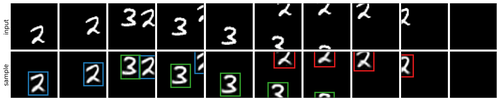
\includegraphics[width=\linewidth]{figures/SQAIR/mnist_rec/in_and_out.png}
    \caption{\gls{SQAIR} trained on a harder version of moving-\textsc{mnist}. Input images (top) and \gls{SQAIR} reconstructions with marked glimpse locations (bottom)}
    \label{fig:mnist_rec_in_and_out}
\end{figure}
	\newpage
	\section{Failure cases of \textsc{sqair}}
\label{app:fail}

\begin{center}
    \centering
    \begin{minipage}[c]{0.65\linewidth}
        \centering
        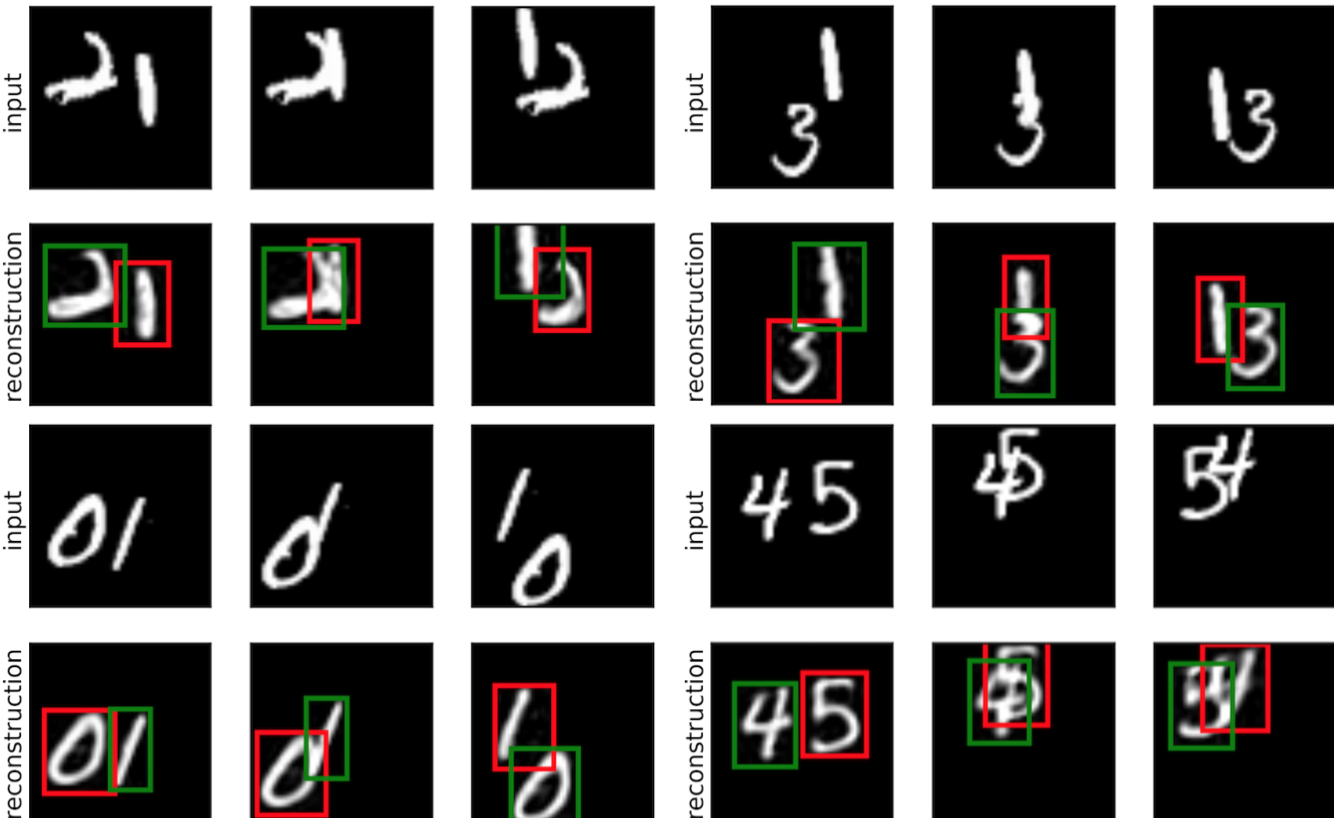
\includegraphics[width=\linewidth]{figures/SQAIR/sqair_id_swap}
    \end{minipage}
    \hfill
    \begin{minipage}[c]{0.33\linewidth}
    \centering
        \captionof{figure}{Examples of ID swaps in a version of \gls{SQAIR} \textit{without} proposal glimpse extraction in \gls{prop} (see \Cref{app:algo} for details). Bounding box colours correspond to object index (or its identity). When \gls{prop} is allowed the same access to the image as \gls{disc}, then it often prefers to ignore latent variables, which leads to swapped inference order.}
        \label{fig:id_swap}
    \end{minipage}
\end{center}
\begin{center}
    \centering
    \begin{minipage}[c]{0.65\linewidth}
        \centering
        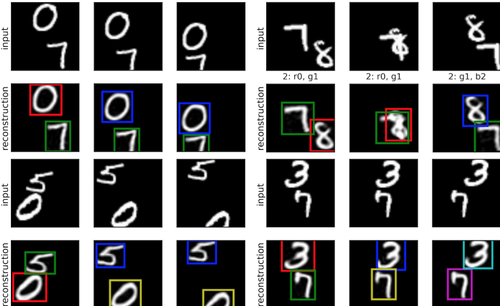
\includegraphics[width=\linewidth]{figures/SQAIR/sqair_redetect}
    \end{minipage}
    \hfill
    \begin{minipage}[c]{0.33\linewidth}
        \centering
        \vspace{8pt}
        \captionof{figure}{Examples of re-detections in \textsc{mlp}-\gls{SQAIR}. Bounding box colours correspond to object identity, assigned to it upon discovery. In some training runs, \gls{SQAIR} converges to a solution, where objects are re-detected in the second frame, and \gls{prop} starts tracking only in the third frame (left). Occasionally, an object can be re-detected after it has severely overlapped with another one (top right). Sometimes the model decides to use only \gls{disc} and repeatedly discovers all objects (bottom right). These failure mode seem to be mutually exclusive -- they come from different training runs.}
        \label{fig:redetect}
    \end{minipage}
\end{center}

\begin{center}
    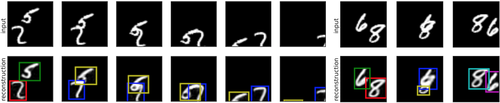
\includegraphics[width=\linewidth]{figures/SQAIR/sqair_weird_rec}
    \captionof{figure}{Two failed reconstructions of \gls{SQAIR}.
        \textit{Left}:
            \Gls{SQAIR} re-detects objects in the second time-step. Instead of 5 and 2, however, it reconstructs them as 6 and 7. Interestingly, reconstructions are consistent through the rest of the sequence.
        \textit{Right:}
            At the second time-step, overlapping 6 and 8 are explained as 6 and a small 0. The model realizes its mistake in the third time-step, re-detects both digits and reconstructs them properly.
    }
    \label{fig:weird_rec}
\end{center}
	\newpage
	\section{Reconstruction and Samples from the Moving-MNIST Dataset}
\label{app:mnist_visual}


\subsection{Reconstructions}
\begin{center}

    % 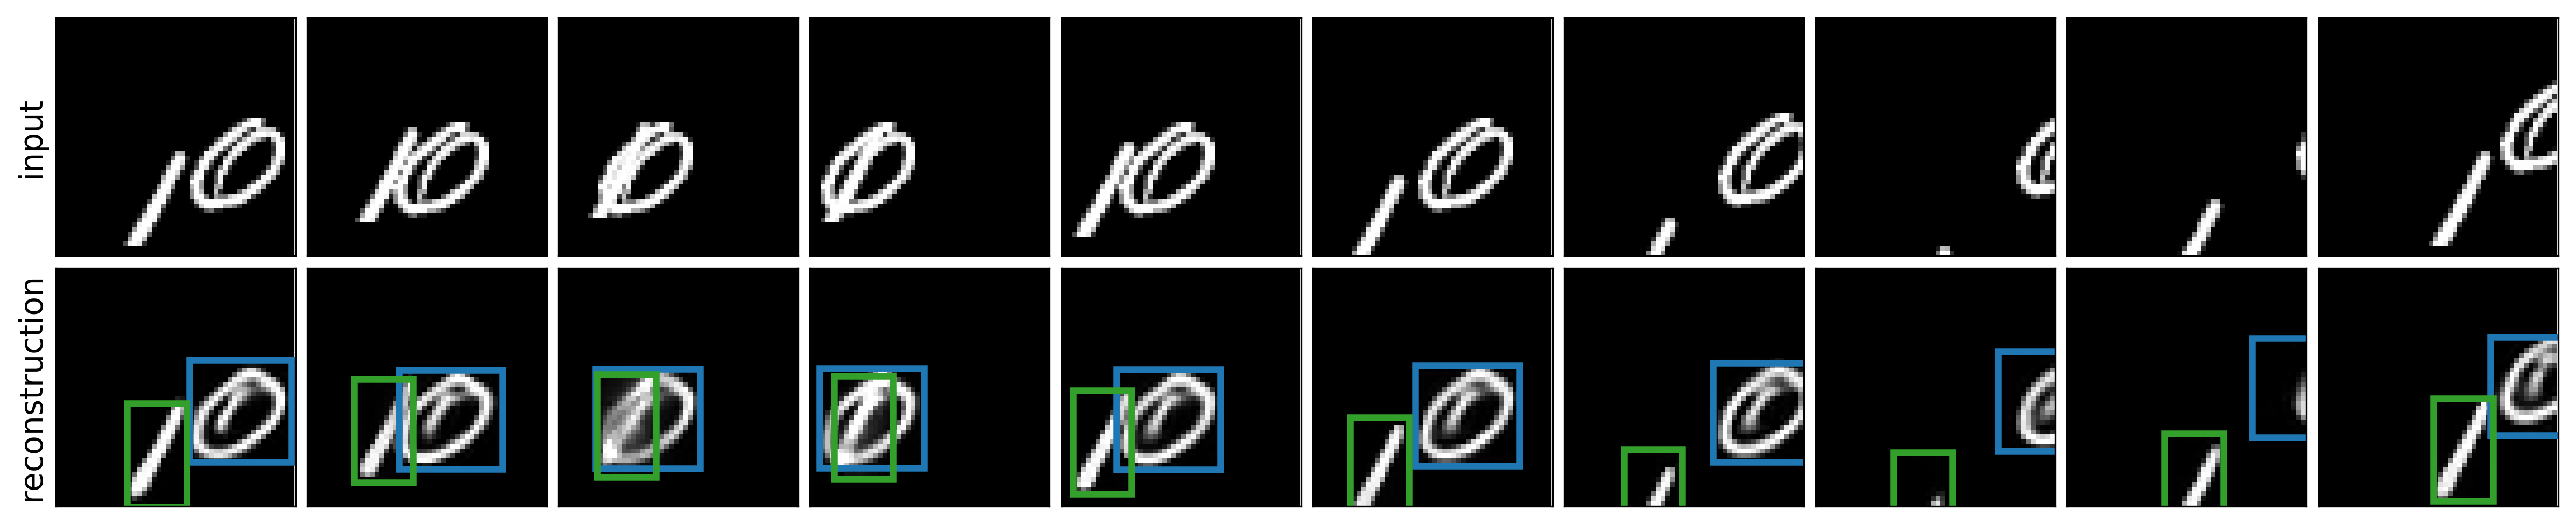
\includegraphics[width=\linewidth]{figures/SQAIR/mnist_rec/000037.png}
    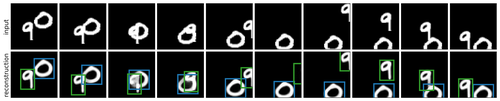
\includegraphics[width=\linewidth]{figures/SQAIR/mnist_rec/000047.png}
    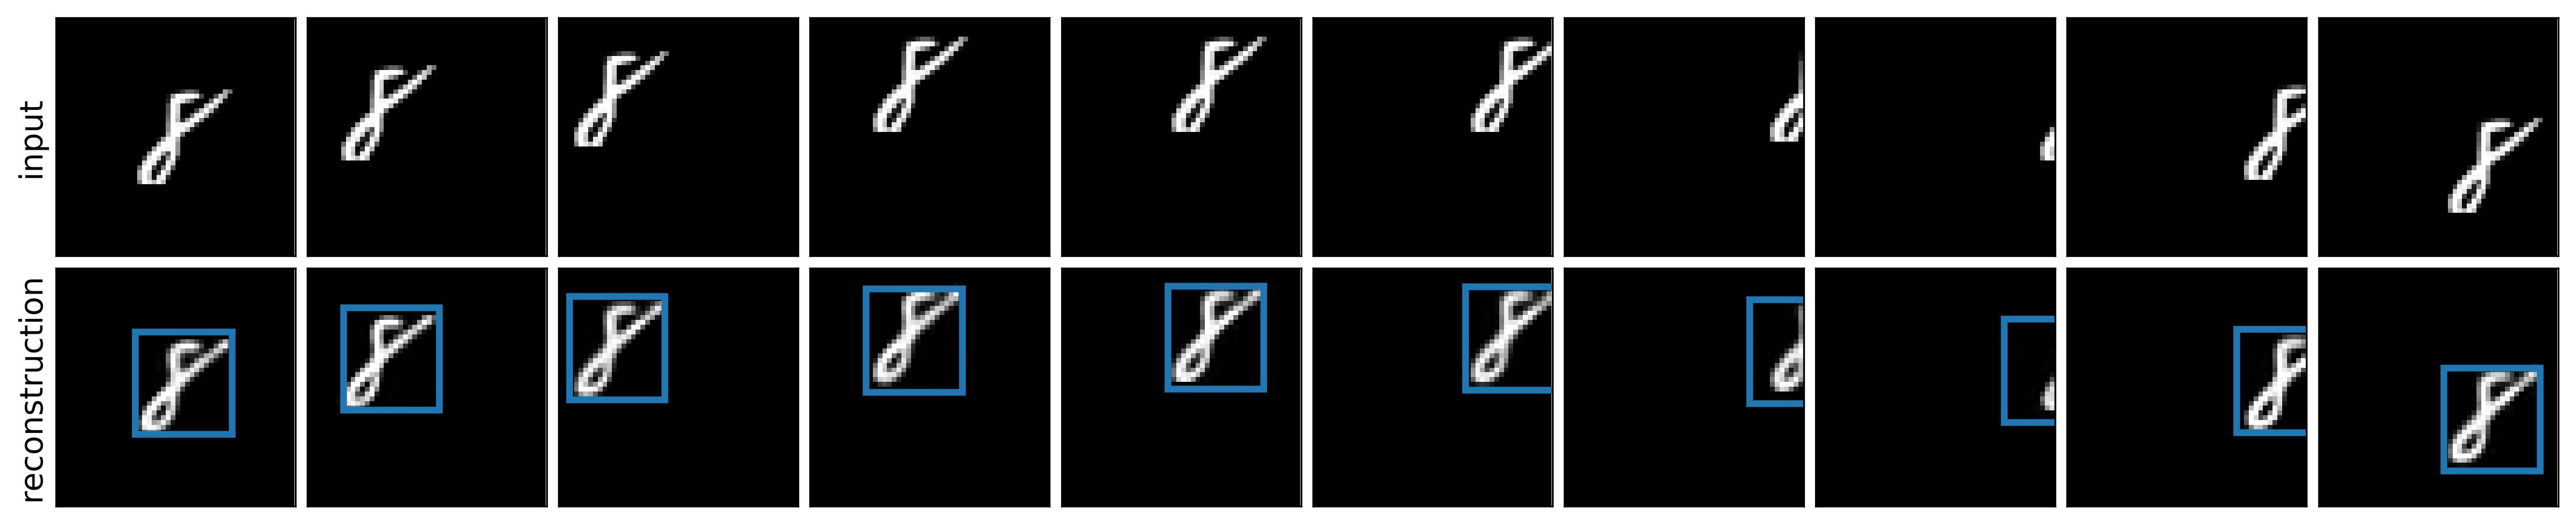
\includegraphics[width=\linewidth]{figures/SQAIR/mnist_rec/000050.png}
    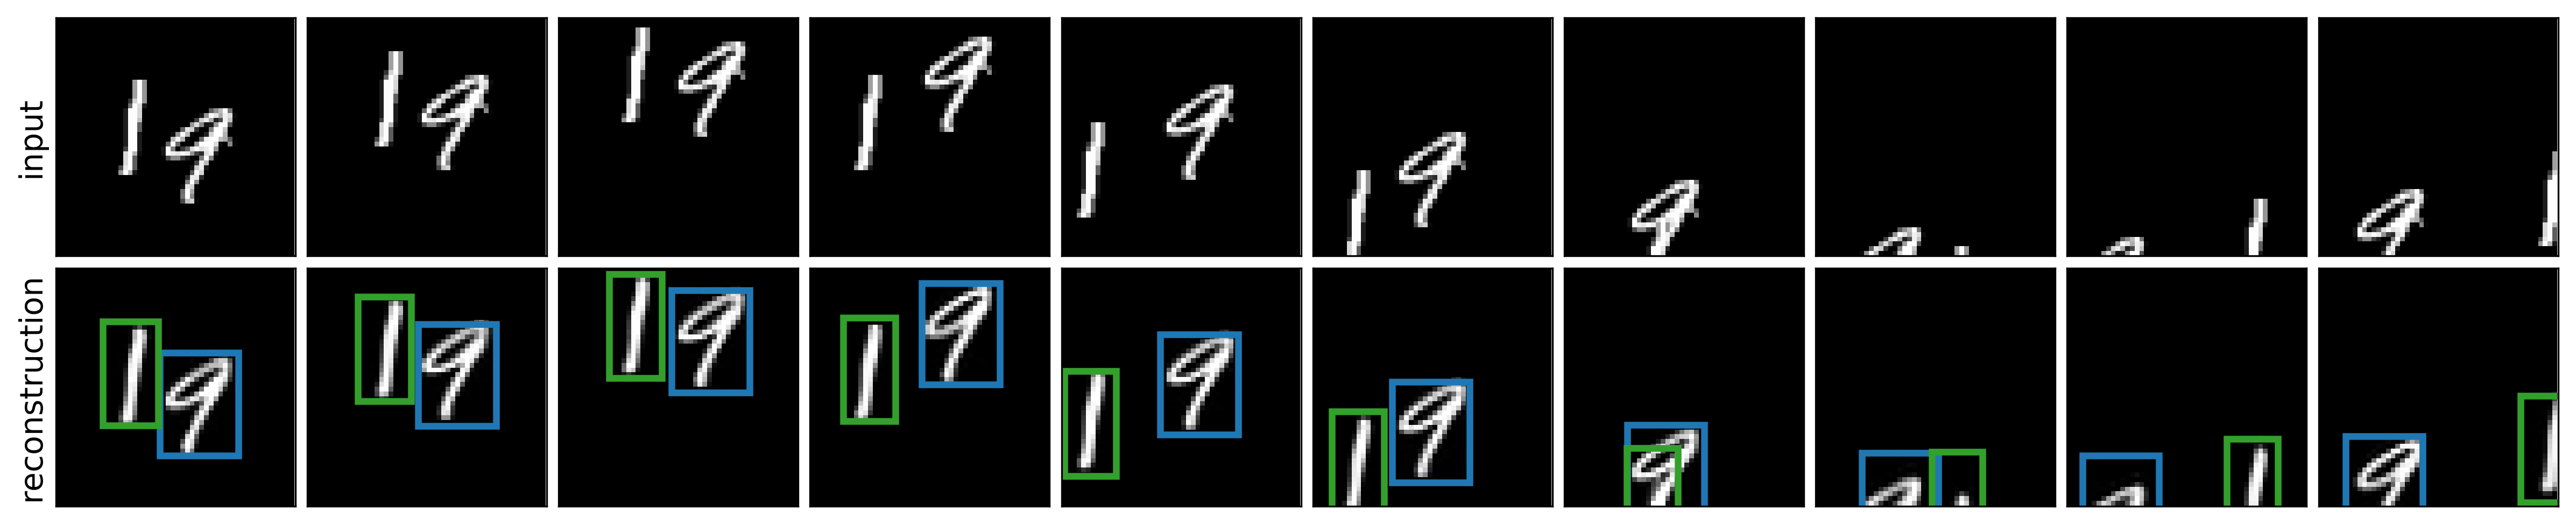
\includegraphics[width=\linewidth]{figures/SQAIR/mnist_rec/000070.png}
    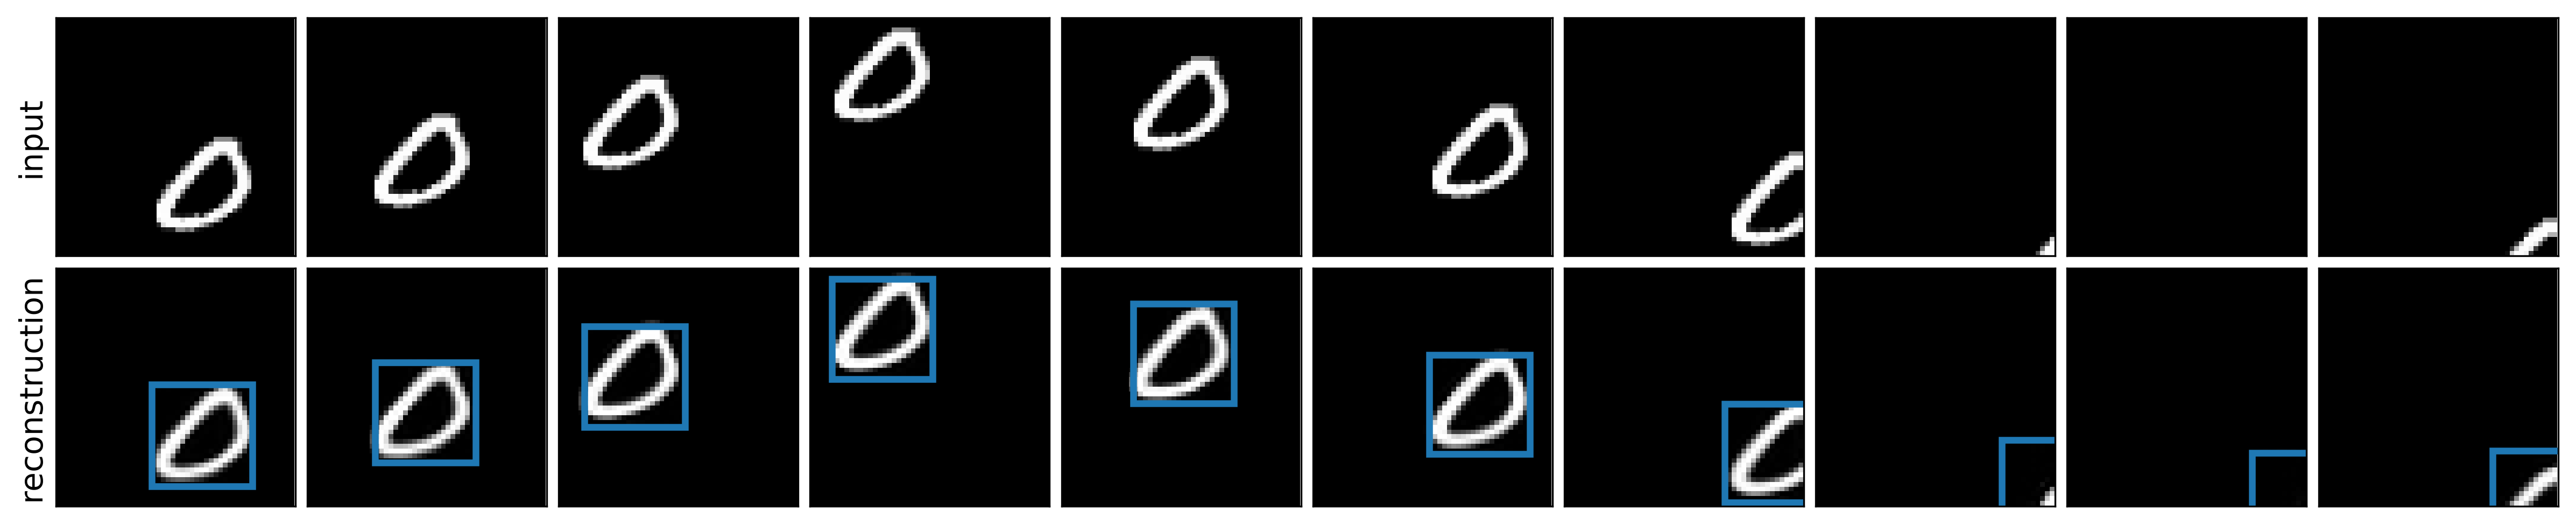
\includegraphics[width=\linewidth]{figures/SQAIR/mnist_rec/000074.png}
    % \includegraphics[width=\linewidth]{figures/SQAIR/mnist_rec/000083.png}
    \includegraphics[width=\linewidth]{figures/SQAIR/mnist_rec/000087.png}
    \includegraphics[width=\linewidth]{figures/SQAIR/mnist_rec/000088.png}
    \includegraphics[width=\linewidth]{figures/SQAIR/mnist_rec/000098.png} 
    \captionof{figure}{Sequences of input (first row) and \gls{SQAIR} reconstructions with marked glimpse locations. Reconstructions are all temporally consistent.}
    \label{fig:mnist_recs_additional}
\end{center}



% \begin{figure}
%     \centering
%     % \includegraphics[width=\linewidth]{figures/SQAIR/mnist_samples_long/000002.png}
%     % \includegraphics[width=\linewidth]{figures/SQAIR/mnist_samples_long/000003.png}
%     % \includegraphics[width=\linewidth]{figures/SQAIR/mnist_samples_long/000005.png}
%     % \includegraphics[width=\linewidth]{figures/SQAIR/mnist_samples_long/000011.png}
%     % \includegraphics[width=\linewidth]{figures/SQAIR/mnist_samples_long/000012.png}
%     \caption{Inputs and reconstructions of length $32$ from \gls{SQAIR} trained for ten time-steps}
%     \label{fig:mnist_recs_long}
% \end{figure}

\begin{center}
    % \includegraphics[width=\linewidth]{figures/SQAIR/vrnn_rec/000004.png}
    % \includegraphics[width=\linewidth]{figures/SQAIR/vrnn_rec/000007.png}
    \includegraphics[width=\linewidth]{figures/SQAIR/vrnn_rec/000009.png}
    \includegraphics[width=\linewidth]{figures/SQAIR/vrnn_rec/000015.png}
    \includegraphics[width=\linewidth]{figures/SQAIR/vrnn_rec/000018.png}
    \includegraphics[width=\linewidth]{figures/SQAIR/vrnn_rec/000038.png}
    \includegraphics[width=\linewidth]{figures/SQAIR/vrnn_rec/000041.png}
    \includegraphics[width=\linewidth]{figures/SQAIR/vrnn_rec/000050.png}
    % \includegraphics[width=\linewidth]{figures/SQAIR/vrnn_rec/000063.png}
    \includegraphics[width=\linewidth]{figures/SQAIR/vrnn_rec/000066.png}
    \captionof{figure}{Sequences of input (first row) and \textsc{conv}-\gls{VRNN} reconstructions. They are not temporally consistent. The reconstruction at time $t=1$ is typically of lower quality and often different than the rest of the sequence.}
    \label{fig:mnist_recs_vrnn}
\end{center}

\subsection{Samples}
\begin{center}
    \includegraphics[width=\linewidth]{figures/SQAIR/mnist_samples/000044.png}
    \includegraphics[width=\linewidth]{figures/SQAIR/mnist_samples/000059.png}
    \includegraphics[width=\linewidth]{figures/SQAIR/mnist_samples/000060.png}
    \includegraphics[width=\linewidth]{figures/SQAIR/mnist_samples/000062.png}
    \includegraphics[width=\linewidth]{figures/SQAIR/mnist_samples/000071.png}
    \includegraphics[width=\linewidth]{figures/SQAIR/mnist_samples/000073.png}
    \includegraphics[width=\linewidth]{figures/SQAIR/mnist_samples/000092.png}
    \includegraphics[width=\linewidth]{figures/SQAIR/mnist_samples/000157.png}
    \includegraphics[width=\linewidth]{figures/SQAIR/mnist_sample_curious/000089.png}
    \captionof{figure}{Samples from \gls{SQAIR}. Both motion and appearance are temporally consistent. In the last sample, the model introduces the third object despite the fact that it has seen only up to two objects in training.}
    \label{fig:mnist_samples_additional}
\end{center}

% \begin{figure}
%     \centering
% %     \includegraphics[width=\linewidth]{figures/SQAIR/mnist_samples_long/000002.png}
% %     \includegraphics[width=\linewidth]{figures/SQAIR/mnist_samples_long/000003.png}
% %     \includegraphics[width=\linewidth]{figures/SQAIR/mnist_samples_long/000005.png}
% %     \includegraphics[width=\linewidth]{figures/SQAIR/mnist_samples_long/000011.png}
% %     \includegraphics[width=\linewidth]{figures/SQAIR/mnist_samples_long/000012.png}
% %     \caption{Samples of length $32$ from \gls{SQAIR} trained for ten time-steps}
%     \label{fig:mnist_samples_long}
% \end{figure}

\newpage
\begin{center}
    \includegraphics[width=\linewidth]{figures/SQAIR/vrnn_samples/000002.png}
    \includegraphics[width=\linewidth]{figures/SQAIR/vrnn_samples/000004.png}
    \includegraphics[width=\linewidth]{figures/SQAIR/vrnn_samples/000007.png}
    \includegraphics[width=\linewidth]{figures/SQAIR/vrnn_samples/000009.png}
    \includegraphics[width=\linewidth]{figures/SQAIR/vrnn_samples/000012.png}
    \includegraphics[width=\linewidth]{figures/SQAIR/vrnn_samples/000013.png}
    \includegraphics[width=\linewidth]{figures/SQAIR/vrnn_samples/000016.png}
    \includegraphics[width=\linewidth]{figures/SQAIR/vrnn_samples/000066.png}
    \includegraphics[width=\linewidth]{figures/SQAIR/vrnn_samples/000084.png}
    \captionof{figure}{Samples from \textsc{conv}-\gls{VRNN}. They show lack of temporal consistency. Objects in the generated frames change between consecutive time-steps and they do not resamble digits from the training set.}
    \label{fig:mnist_samples_vrnn}
\end{center}
% \end{figure}

\newpage
\subsection{Conditional Generation}

\begin{center}
    % \includegraphics[width=\linewidth]{figures/SQAIR/mnist_cond_gen/000004.png}
    % \includegraphics[width=\linewidth]{figures/SQAIR/mnist_cond_gen/000005.png}
    % \includegraphics[width=\linewidth]{figures/SQAIR/mnist_cond_gen/000006.png}
    % \includegraphics[width=\linewidth]{figures/SQAIR/mnist_cond_gen/000012.png}
    % \includegraphics[width=\linewidth]{figures/SQAIR/mnist_cond_gen/000019.png}
    % \includegraphics[width=\linewidth]{figures/SQAIR/mnist_cond_gen/000023.png}
    % % \includegraphics[width=\linewidth]{figures/SQAIR/mnist_cond_gen/000026.png}
    % \includegraphics[width=\linewidth]{figures/SQAIR/mnist_cond_gen/000030.png}
    \includegraphics[width=\linewidth]{figures/SQAIR/sqair_mnist_cond_gen_appendix}
    \captionof{figure}{Conditional generation from \gls{SQAIR}, which sees only the first three frames in every case. Top is the input sequence (and the remaining ground-truth), while bottom is reconstruction (first three time-steps) and then generation.}
    \label{fig:mnist_cond_gen_sqair}
\end{center}
	\section{Reconstruction and Samples from the DukeMTMC Dataset}
\label{app:duke_visual}

\begin{center}
    \begin{minipage}[c]{0.49\linewidth}
        \centering
        \includegraphics[width=\linewidth]{figures/SQAIR/duke_rec/000093.png}
        \includegraphics[width=\linewidth]{figures/SQAIR/duke_rec/000045.png}
        \includegraphics[width=\linewidth]{figures/SQAIR/duke_rec/000047.png}
        \includegraphics[width=\linewidth]{figures/SQAIR/duke_rec/000081.png}
        \includegraphics[width=\linewidth]{figures/SQAIR/duke_rec/000085.png}
    \end{minipage}
    \hfill
    \begin{minipage}[c]{0.49\linewidth}
        \centering
        \includegraphics[width=\linewidth]{figures/SQAIR/duke_rec/000088.png}
        \includegraphics[width=\linewidth]{figures/SQAIR/duke_rec/000046.png}
        \includegraphics[width=\linewidth]{figures/SQAIR/duke_rec/000094.png}
        \includegraphics[width=\linewidth]{figures/SQAIR/duke_rec/000096.png}
        \includegraphics[width=\linewidth]{figures/SQAIR/duke_rec/000108.png}
    \end{minipage}
    \captionof{figure}{Sequences of input (first row) and \gls{SQAIR} reconstructions with marked glimpse locations. While not perfect (spurious detections, missed objects), they are temporally consistent and similar in appearance to the inputs.}
    \label{fig:duke_recs_additional}
\end{center}

\begin{center}
    \begin{minipage}[c]{0.49\linewidth}
        \centering
         \includegraphics[width=\linewidth]{figures/SQAIR/duke_sample/000078.png}
        \includegraphics[width=\linewidth]{figures/SQAIR/duke_sample/000250.png}
        \includegraphics[width=\linewidth]{figures/SQAIR/duke_sample/000005.png}
        \includegraphics[width=\linewidth]{figures/SQAIR/duke_sample/000015.png}
        \includegraphics[width=\linewidth]{figures/SQAIR/duke_sample/000019.png}
        \includegraphics[width=\linewidth]{figures/SQAIR/duke_sample/000023.png}
        \includegraphics[width=\linewidth]{figures/SQAIR/duke_sample/000038.png}
        \includegraphics[width=\linewidth]{figures/SQAIR/duke_sample/000062.png}
    \end{minipage}
    \hfill
    \begin{minipage}[c]{0.49\linewidth}
        \centering
            \includegraphics[width=\linewidth]{figures/SQAIR/duke_sample/000225.png}
        \includegraphics[width=\linewidth]{figures/SQAIR/duke_sample/000121.png}
        \includegraphics[width=\linewidth]{figures/SQAIR/duke_sample/000128.png}
        \includegraphics[width=\linewidth]{figures/SQAIR/duke_sample/000132.png}
        \includegraphics[width=\linewidth]{figures/SQAIR/duke_sample/000134.png}
        \includegraphics[width=\linewidth]{figures/SQAIR/duke_sample/000140.png}
        \includegraphics[width=\linewidth]{figures/SQAIR/duke_sample/000144.png}
    \end{minipage}
    \captionof{figure}{Samples with marked glimpse locations from \gls{SQAIR} trained on the DukeMTMC dataset. Both appearance and motion is spatially consistent. Generated objects are similar in appearance to pedestrians in the training data. Samples are noisy, but so is the dataset.}
    \label{fig:duke_samples_additional}
\end{center}

\begin{center}
    \includegraphics[width=\linewidth]{figures/SQAIR/duke_cond_gen/sqair_duke_cond_gen_appendix.png}
    \captionof{figure}{Conditional generation from \gls{SQAIR}, which sees only the first four frames in every case. Top is the input sequence (and the remaining ground-truth), while bottom is reconstruction (first four time-steps) and then generation.}
    \label{fig:duke_cond_gen_sqair}
\end{center}
\end{subappendices}


\chapter{Stacked Capsule Autoencoders}
\label{ch:sca}

\vspace*{-1em}
\begin{abstract}
\vspace*{-.5em}





%Any object can be seen as a geometrically organized set of interrelated parts. Capsule networks model object parts explicitly and use them to predict whole objects. Typically, capsules are trained discriminatively and assume that an object exists if it is predicted by several parts at the same time, while an iterative inference procedure ensures that a single part is not assigned to multiple objects. We devise an unsupervised version, that consists of a two-stage, stacked capsule autoencoder:
% 
% the first stage is responsible for segmenting images into parts and their poses, while the second stage organizes these already-discovered parts into objects and their poses.
% The bottom (\!\ie first) stage is trained to reconstruct the original image as a mixture of discovered parts.
% The top stage is  trained to reconstruct part poses as  mixtures of predictions made by different objects.
% the bottom stage is responsible for segmenting images into parts and is trained to reconstruct the original image as a mixture of the already discovered parts. The top stage organizes these parts into objects and their poses; it is trained to reconstruct part poses as a mixture of predictions made by different objects.
% The top-level decoder predicts the poses of the parts by applying explicitly-parametrized affine transformations to the object pose parameters. These coordinate transformations do not depend on viewpoint, so learning them can be used to acquire viewpoint-invariant knowledge in a statistically efficient manner. We learn objects and their parts on unlabeled data, and when told the names of the learned classes, we achieve state-of-the-art results for unsupervised classification on \textsc{svhn} (55\%) and near state-of-the-art on \textsc{mnist} (98.5\%).
An object can be seen as a geometrically organized set of interrelated parts.
A system that makes explicit use of these geometric relationships to recognize objects should be naturally robust to changes in viewpoint, because the intrinsic geometric relationships are viewpoint-invariant.
We describe an unsupervised version of capsule networks, in which a neural encoder, which looks at all of the parts, is used to infer the presence and poses of object capsules.
The encoder is trained by backpropagating through a decoder, which predicts the pose of each already discovered part using a mixture of pose predictions.
%each of which is computed from the pose of a proposed object and the learned object->part relationship. 
The parts are discovered directly from an image, in a similar manner, by using a neural encoder, which infers parts and their affine transformations.
The corresponding decoder models each image pixel as a mixture of predictions made by affine-transformed parts.
%that are learned for each part.  
We learn object- and their part-capsules on unlabeled data, and then cluster the vectors of presences of object capsules.
When told the names of these clusters, we achieve state-of-the-art results for unsupervised classification on \textsc{svhn} (55\%) and near state-of-the-art on \textsc{mnist} (98.5\%).
\end{abstract}

% Any object can be seen as a geometrically organized set of interrelated parts.
% Capsule networks model object parts explicitly and use them to predict whole objects.
% Typically, capsules are trained discriminatively and assume that an object exists if it is predicted by several parts at the same time; an iterative inference procedure ensures that a single part is not assigned to multiple objects.
% We devise an unsupervised version, that consists of a two-stage, stacked capsule autoencoder: the first stage is responsible for segmenting images into parts and their poses, while the second stage organizes these already-discovered parts into objects and their poses.
% The bottom (\!\ie first) stage is trained to reconstruct the original image as a mixture of discovered parts.
% The top stage is  trained to reconstruct part poses as  mixtures of predictions made by different objects.
% The top-level decoder predicts the poses of the parts by applying explicitly-parametrized affine transformations to the object pose parameters.
% These coordinate transformations do not depend on viewpoint, so learning them can be used to acquire viewpoint-invariant knowledge in a statistically efficient manner. We learn objects and their parts on unlabeled data, and when told the names of the learned classes, we achieve state-of-the-art results for unsupervised classification on \textsc{svhn} (55\%) and near state-of-the-art on \textsc{mnist} (98.5\%).

%\vspace*{-1em}
%\section{Introduction}
% \Glspl{CNN} for image classification learn faster and generalize better than non-convolutional ones, because convolutions reduce the number of learned parameters and inject a strong and generally correct inductive bias: 
% if a local feature is useful in one image location, the same feature is likely to be useful in other locations.
% It is tempting to embed even stronger inductive biases by replicating features across scale, orientation and other affine degrees of freedom, but this quickly leads to cumbersome high-dimensional feature maps \citep{Cohen2016steerable}.
% 
\Gls{CNN} work better than networks without weight-sharing because of their inductive bias: if a local feature is useful in one image location, the same feature is likely to be useful in other locations. It is tempting to exploit other effects of viewpoint changes by replicating features across scale, orientation and other affine degrees of freedom, but this quickly leads to cumbersome high-dimensional feature maps. %%\citep{Cohen2016steerable}.
%% its a bit mean to blame taco and max for this and we refer to them later anyway.

An alternative to replicating features across the non-translational degrees of freedom is to explicitly learn transformations between the natural coordinate frame of a whole object and the natural coordinate frames of each of its parts.   Computer graphics relies on such object$\rightarrow$part coordinate transformations to represent the geometry of an object in a viewpoint-invariant manner. Moreover, there is strong evidence that, unlike standard \gls{CNN}s, human vision also relies on coordinate frames: imposing an unfamiliar coordinate frame on a familiar object makes it difficult to recognize the object or its geometry \citep{Rock73, Hinton79}.

A neural system can learn to reason about transformation between objects, their parts and the viewer, but each of the transformations is likely to require different representation.
An \gls{OP} is viewpoint-invariant and is naturally coded by learned weights.  
The relationship of an object or part to the viewer changes with the viewpoint (it is viewpoint-equivariant) and is naturally coded using neural activations\footnote{
    This may explain why accessing perceptual knowledge about objects, when they are not visible, requires creating a mental image of the object with a specific viewpoint.
}.
With this representation, pose of a single object is represented by its relationship to the viewer.
Consequently, representing a single object does not necessitate replicating neural activations across space, unlike in \glspl{CNN}.
It is only processing two (or more) different instances of the same type of object in parallel that requires spatial replicas of both model parameters and neural activations.
% So the stride of the replication of object and part capsules can be determined by the sparsity of that type of object or part in the image and can typically be much larger for more complex objects because they are sparser. 

In this paper we propose the \gls{SCAu}, which has two stages (\cref{fig:capsule_arch}). The first stage, the \gls{PCAu}, segments an image into constituent parts, infers their poses, and reconstructs each image pixel as a mixture of the pixels of transformed part templates.
The second stage, the \gls{OCAu}, tries to organize discovered parts and their poses into a smaller set of objects that can explain the part poses using a separate mixture of predictions for each part. 
Every object capsule contributes components to each of these mixtures by multiplying its pose---the \gls{OV}---by the relevant \glsreset{OP}\gls{OP}\footnote{The type of a part capsule may determine which, if any, of an object's parts contribute to the mixture used to model the pose of an already discovered part}.

Stacked Capsule Autoencoders (\Cref{sec:caps_decoders}) capture spatial relationships between whole objects and their parts when trained on unlabelled data.
The vectors of presence probabilities for the object capsules tend to form tight clusters, and when we assign a class to each cluster we achieve state-of-the-art results for unsupervised classification on \textsc{svhn} (55\%) and near state-of-the-art on \textsc{mnist} (98.5\%), which can be further improved to 67\% and 99\%, respectively, by learning fewer than 300 parameters. We also present promising proof-of-concept results on \textsc{cifar10} (\Cref{sec:sca_experiments}).
%
We describe related work in \Cref{sec:related_work} and discuss implications of our work and future  directions in \Cref{sec:sca_discussion}.

\begin{figure}
%    \centering
%    \begin{minipage}[c]{0.68\linewidth}
        \centering
        \includegraphics[width=.68\linewidth]{figures/SCA/blocks_v4}
        % \vspace*{-1.5em}
%    \end{minipage}
%    \hfill
%    \begin{minipage}[c]{0.3\linewidth}
%        \centering
        \caption{
            Stacked Capsule Autoencoder (\textsc{scae}):
            % \arcfull{}{SCA}
            (a) \textit{part} capsules segment the input into parts and their poses. The poses are then used to reconstruct the input by affine-transforming learned templates.
            (b) \textit{object} capsules try to arrange inferred poses into objects, thereby discovering underlying structure.
            \textsc{scae} is trained by maximizing image and part log-likelihoods subject to sparsity constraints.
        }
        \label{fig:capsule_arch}
        % \vspace*{-1.5em}
%    \end{minipage}
%    \vspace*{-.75em}
\end{figure}

% \Gls{SCA} has two stages (\cref{fig:capsule_arch}).
% Its first (\!\ie bottom) stage, \gls{ICAE}, segments an image into constituent parts, infers their poses, and reconstructs the image as a mixture of transformed parts.
% The second (top) stage, \gls{CAE}, tries to organize discovered parts and their poses into objects, where part poses \apart{} are derived from mixtures of predictions made by objects \awhole{}.
% Since each part is explained by a separate mixture, we do not need to route predictions between mixtures.
% This justifies dispensing with iterative procedures during inference, which can now be amortized using an arbitrary feed-forward encoder.
% The encoder's ability to deal with different viewpoints is not built-in; instead it is learned by doing inference for the affine-aware decoder.
% As \gls{SCA} is unsupervised, it can leverage potentially unlimited amounts of unlabelled data.
% % \yw{maybe say that the model is an autoencoder, where the decoder is structured with the assumptions about the geometries of objects as before? also maybe give some intuition about the decoder structuring the encoder to learn the structure we want it to learn (not sure if that makes sense)?}


\section{Stacked Capsule Autoencoders (\textsc{SCAE})}
\label{sec:caps_decoders}
Segmenting an image into parts is non-trivial, so we begin by abstracting away pixels and the part-discovery stage, and develop the \gls{CCAu} (\Cref{sec:constellation}).
It uses two-dimensional points as parts, and their coordinates are given as the input to the system. \Gls{CCAu} learns to model sets of points as arrangements of familiar constellations, each of which has been transformed by an independent similarity transform. The \gls{CCAu} learns to assign individual points to their respective constellations—without knowing the number of constellations or their individual shapes in advance.  Next, in Section 2.2, we develop the \glsreset{PCAu}\gls{PCAu} which learns to infer parts and their poses from images. Finally, we stack the \glsreset{OCAu}\gls{OCAu}, which closely resembles the \gls{CCAu}, on top of the \gls{PCAu} to form the \glsreset{SCAu}\gls{SCAu}.



\subsection{Constellation Autoencoder (\textsc{CCAE})}
\label{sec:constellation}

Let $\set{\bx_m\mid m=1,\dots,M}$ be a set of two-dimensional input points, where every point belongs to a constellation as in \Cref{fig:constellations}.
We first encode all input points (which take the role of part capsules) with Set Transformer \citep{Lee2019set}---a permutation-invariant encoder $h^\mathrm{caps}$ based on attention mechanisms---into $K$ object capsules.
An object capsule $k$ consists of a capsule feature vector $\bc_k$, its presence probability $a_k \in \interval{0, 1}$ and a $3 \times 3$ \glsreset{OV}\gls{OV} matrix, which represents the affine transformation between the object (constellation) and the viewer.
Note that each object capsule can represent only one object at a time.
Every object capsule uses a separate \gls{MLP} $\operatorname{h_k^\mathrm{part}}$ to predict $N \leq M$ part candidates from the capsule feature vector $\bc_k$.
Each candidate consists of the conditional probability $a_{k,n} \in \interval{0, 1}$ that a given candidate part exists, an associated scalar standard deviation $\lambda_{k,n}$, and a $3 \times 3$ \glsreset{OP}\gls{OP} matrix, which represents the affine transformation between the object capsule and the candidate part\footnote{Deriving these matrices from the capsule feature vector allows for deformable objects. We model \gls{OP}s as the sum of an input-dependent component and a constant bias. We encourage different capsules to specialize to different constellations by putting a strong $L_2$ penalty on the former.}.
Candidate predictions $\mu_{k,n}$ are given by the product of the object capsule \gls{OV} and the candidate \gls{OP} matrices.
We then model each input part as a Gaussian mixture, where $\mu_{k,n}$ and $\lambda_{k,n}$ are the centers and standard deviations of the isotropic components.
See \Cref{fig:capsule_arch,fig:sca_arch} for illustration; formal description follows:
\begin{align}
    &\textsc{ov}_{1:K}, \bc_{1:K}, a_{1:K} = \operatorname{h^\mathrm{caps}} (\bx_{1:M}) &\text{encode object capsule parameters,}\\
    % 
    &\textsc{op}_{k,1:N}, a_{k, 1:N}, \lambda_{k, 1:N} = \operatorname{h_k^\mathrm{part}} (\bc_k) &\text{decode candidate parameters from $c_k$'s,}\\
    % 
    &V_{k,n} = \textsc{ov}_k \textsc{op}_{k,n} &\text{decode a part pose candidate,}\\
    % 
    &\p{\bx_m}{k,n} = \gauss{\bx_m \mid \mu_{k,n}, \lambda_{k,n}} &\text{turn candidates into mixture components,}\label{eq:component}
\end{align}
\begin{equation}
    \p{\bx_{1:M}} = \prod_{m=1}^M \sum_{k=1}^K \sum_{n=1}^{N}  
    \frac{a_k a_{k,n}}{\sum_i a_i \sum_j a_{i,j}}
    \,\p{\bx_m}{k,n}\,. \label{eq:constellation_likelihood}
\end{equation}
The model is trained without supervision by maximizing the likelihood of part capsules in \Cref{eq:constellation_likelihood} subject to sparsity constraints, \textit{cf}.\ \Cref{sec:losses}.
The part capsule $m$ can be assigned to the object capsule $k^\star$ as $k^\star = \operatorname{arg\,max}_{k}~a_k a_{k,n}\;\p{\bx_m}{k,n}$.\footnote{We treat parts as independent and evaluate their probability under the same mixture model. While there are no clear 1:1 connections between parts and predictions, it seems to work well in practice.}
%\begin{figure} 
%    \centering
%    \begin{minipage}[c]{0.35\linewidth}
%        \centering
%        \includegraphics[width=\linewidth]{figures/SCA/consinvert5}
%    \end{minipage}
%    \hfill
%    \begin{minipage}[c]{0.63\linewidth}
%        \centering
%        \caption{
%            Unsupervised segmentation of points belonging to up to three constellations of squares and triangles at different positions, scales and orientations. 
%            The model is trained to reconstruct the points (top row) under the \gls{CCAu} mixture model. The bottom row colors the points based on the parent with highest posterior probability in the mixture model. 
%            The right-most column shows a failure case.
%            Note that the model uses sets of points, not pixels, as its input; we use images  only to visualize the constellation arrangements.
%        }
%        \label{fig:constellations}
%    \end{minipage}
%\end{figure}
\begin{SCfigure}[50]
	\centering
%	\begin{minipage}[c]{0.35\linewidth}
%		\centering
		\includegraphics[width=.35\linewidth]{figures/SCA/consinvert5}
%	\end{minipage}
%	\hfill
%	\begin{minipage}[c]{0.63\linewidth}
%		\centering
		\caption{
			Unsupervised segmentation of points belonging to up to three constellations of squares and triangles at different positions, scales and orientations. 
			The model is trained to reconstruct the points (top row) under the \gls{CCAu} mixture model. The bottom row colors the points based on the parent with highest posterior probability in the mixture model. 
			The right-most column shows a failure case.
			Note that the model uses sets of points, not pixels, as its input; we use images  only to visualize the constellation arrangements.
		}
		\label{fig:constellations}
%	\end{minipage}
\end{SCfigure}
Empirical results show that this model is able to perform unsupervised instance-level segmentation of points belonging to different constellations, even in data which is difficult to interpret for humans. See \Cref{fig:constellations} for an example and \Cref{sec:constellation_expr} for details.

\subsection{Part Capsule Autoencoder (\textsc{PCAE})}
\label{sec:img_capsule}
Explaining images as geometrical arrangements of parts requires first inferring what parts the images are composed of, as well as the relationships of the parts to the viewer (which we call their poses). For the \gls{CCAu} a part is just a 2D point, but here each part capsule has a six \gls{DOF} pose, a presence variable and a unique identity. We frame the part-discovery problem as auto-encoding: the encoder learns to infer the poses and presences of different part capsules, while the decoder learns an image template for each part (\cref{fig:learned_templates}) similar to \cite{Tieleman2014thesis,Eslami2016air}. The templates corresponding to present parts are affine-transformed using their poses, and the pixels of these transformed templates are used to create a separate mixture model for each image pixel.
The \gls{PCAu} is followed by an \glsreset{OCAu}\gls{OCAu}, which closely resambles the \gls{CCAu} and is described in \Cref{sec:ocae}.

Let $\by \in \interval{0, 1}^{h \times w \times c}$ be the image.
We limit the maximum number of part capsules to $M$ and use an encoder to infer their poses $\bx_m \in \RR^6$, presence probabilities $d_m \in \interval{0, 1}$, and special features $\bz_m \in \RR^{c_z}$, one per part capsule.
The latter do not take part in direct image reconstruction, but inform the \gls{OCAu} about special aspects of the corresponding part; they are trained by backpropagating derivatives from the \gls{OCAu}.

At present, we do not allow multiple occurrences of the same type of part in an image, so the part capsules themselves are not replicated across space, though they could be.
However, we do need to recognize the part wherever it occurs in the image, and therefore the encoder consists of a \gls{CNN} with a bottom-up attention mechanism; for every part capsule $k$, it predicts a feature map $\bf{e}_k$ of $6 \text{\,(pose)} + 1 \text{\,(presence)} + c_z \text{\,(special features)}$ capsule parameters with spatial dimensions $h_e \times w_e$\,, as well as a single-channel attention mask $\bf{a}_k$.
The final parameters for that capsule are computed as $\sum_{i} \sum_j \bf{e}_{k, i,j} \operatorname{softmax}(\bf{a})_{k,i,j}$, where $\operatorname{softmax}$ is along the spatial dimensions.
This is similar to global average pooling, but allows some spatial locations to contribute to the final result more than others; we call this approach \textit{attention-based pooling}. Its effect on the model performance is analyzed in \Cref{sec:ablation}.

The image pixels are modelled as independent Gaussian mixtures.
For every pixel, we take the corresponding pixels of the transformed templates and treat them as centers of isotropic Gaussian components with constant variance.
Their mixing probabilities are proportional to both presence probabilities of part capsules and a function $f_c: \RR^c \mapsto \interval{0, 1}$ of the color value at that location\footnote{
Templates are assumed to be sparse; if there exists a template that has a non-zero value at a given location, then this templates should be used.}, where $c$ is the number of image channels. 
More formally:
\begin{align}
    &\bx_{1:M}, d_{1:M}, \bz_{1:M} = \operatorname{h^{\mathrm{enc}}}(\by) \qquad\text{encode the image to part capsule params,}\\
    &\widehat{T}_m = \operatorname{TransformImage} (T_m, \bx_m)  \qquad\text{affine transforms image templates,}\\
    % 
    &p^y_{m,i,j} \propto d_m \operatorname{f_c}\left(\widehat{T}_{m,i,j}\right) \qquad\text{compute mixing probabilities,}\\
    % 
    &\p{\by} = \prod_{i,j} \sum_{m=1}^M p^y_{m,i,j}\, \gauss{y_{i,j} \mid \widehat{T}_{m,i,j}, \sigma^2_y} \qquad\text{calculate image likelihood.} \label{eq:im_likelihood}
\end{align}

\subsection{Object Capsule Autoencoder (\textsc{OCAE})}
\label{sec:ocae}
% \todo{\ak{explain why constellation and object aes are differnet}}

The next step is to find objects in the already discovered parts\footnote{
    Discovered objects are {\it not} used top-down to refine the presences or poses of the parts during inference. However, the derivatives backpropagated via \gls{OCAu} refine the lower-level encoder network that infers the parts.
}.
To do so, we use concatenated poses $\bx_m$, special features $\bz_m$ and flattened templates $T_m$ (which convey the identity of the part capsule)
as an input to the \gls{OCAu}, which differs from the \gls{CCAu} in the following ways.
Firstly, we feed part capsule presence probabilities $d_m$ into the \gls{OCAu}'s encoder---these are used to bias the Set Transformer's attention mechanism to not take absent points into account.
% ; see \Cref{app:set_transformer} for details.
Secondly, $d_m$'s are also used to weigh the part-capsules' log-likelihood, \textit{cf}. \Cref{eq:constellation_likelihood}.
Additionally, we stop the gradient on all of \gls{OCAu}'s inputs except the special features to improve training stability and avoid the problem of collapsing latent variables; see\eg \cite{Rasmus2015ladder}.
Finally, parts discovered by the \gls{PCAu} have independent identities (templates and special features rather than 2D points).
Therefore, every part-pose is explained as an independent mixture of predictions from object-capsules---where every object capsule makes exactly $M$ candidate predictions $V_{k,1:M}$, or exactly {\bf one} candidate prediction per part.
Consequently, the part-capsule likelihood is given by,
\begin{equation}
    \p{\bx_{1:M}, d_{1:M}} = \prod_{m=1}^M \left[\, \sum_{k=1}^K  
    \frac{a_k a_{k,m}}{\sum_i a_i \sum_j a_{i,j}}
    \,\p{\bx_m}{k,m}\right]^{d_m}\,. \label{eq:mod_constellation_likelihood}
\end{equation}

%\begin{figure}
%    \centering
%    \begin{minipage}[b]{.47\linewidth}
%    \includegraphics[width=\linewidth]{figures/SCA/templates}
%    \end{minipage}
%    \hfill
%    \begin{minipage}[b]{.52\linewidth}
%    \caption{Templates learned on \textsc{mnist} (left) as well as sobel-filtered \textsc{svhn} (middle) and \textsc{cifar10} (right). In each case templates converge to strokes. For \textsc{svhn} they often take the form of double strokes---this is due to sobel filtering, which effectively extracts edges.}
%    \label{fig:learned_templates}
%    \end{minipage}
%\end{figure}
\begin{figure}
	\centering
		\includegraphics[width=.85\linewidth]{figures/SCA/templates}
		\caption{Templates learned on \textsc{mnist} (left) as well as sobel-filtered \textsc{svhn} (middle) and \textsc{cifar10} (right). In each case templates converge to strokes. For \textsc{svhn} they often take the form of double strokes---this is due to sobel filtering, which effectively extracts edges.}
		\label{fig:learned_templates}
\end{figure}
\begin{figure}
    \centering
    \begin{subfigure}[c]{.09\linewidth}
        \includegraphics[width=\linewidth]{figures/SCA/mnist/inputs}
        \caption{}
    \end{subfigure}
    \hfill
    \begin{subfigure}[c]{.09\linewidth}
        \includegraphics[width=\linewidth]{figures/SCA/mnist/recs}
        \caption{}
    \end{subfigure}
        \hfill
    \begin{subfigure}[c]{.059\linewidth}
        \includegraphics[width=\linewidth]{figures/SCA/mnist/acts}
        \caption{}
    \end{subfigure}
    \hfill
    \begin{subfigure}[c]{.18\linewidth}
        \includegraphics[width=\linewidth]{figures/SCA/mnist/caps_recs}
        \caption{}
    \end{subfigure}
    \hfill
    \begin{subfigure}[c]{.45\linewidth}
        \includegraphics[width=\linewidth]{figures/SCA/mnist/transformed_templates}
        \caption{}
    \end{subfigure}
%    \hfill
%    \begin{minipage}[c]{.52\linewidth}
        \caption{
        $40\times40$ \textsc{mnist} (a) images and their (b) reconstructions from part capsules in red and object capsules in green, with overlapping regions in yellow.
        Only a few object capsules are activated for every input (c) a priori (left) and even fewer are needed to reconstruct it (right).
        The most active capsules (d) capture object identity and the majority of information about its appearance. 
        Finally, (e) affine-transformed templates show how exactly parts are used to reconstruct the images.
        }
        \label{fig:mnist_rec}
%    \end{minipage}
\end{figure}
\subsection{Achieving Sparse and Diverse Capsule Presences}
\label{sec:losses}
Stacked Capsule Autoencoders are trained to maximise pixel and part log-likelihoods ($\loss[\mathrm{ll}]{} = \log\p{\by} + \log\p{\bx_{1:M}}$).
If not constrained, however, they tend to either use all of the part and object capsules to explain every data example, or collapse onto using always the same subset of capsules, regardless of the input.
We would like the model to use different sets of part-capsules for different input examples and to specialize object-capsules to particular arrangements of parts; to encourage this, we impose sparsity and entropy constraints.  We evaluate their importance in \Cref{sec:ablation}.

We first define prior and posterior object-capsule presence as follows.
For a minibatch of size {\small$B$} with {\small$K$} object capsules and $M$ part capsules we define a minibatch of prior capsule presence $a^\mathrm{prior}_{1:K}$ with dimension {\small$[B, K]$} and posterior capsule presence $a^\mathrm{posterior}_{1:K,1:M}$ with dimension {\small$[B, K, M]$} as,
\begin{equation}
    a^\mathrm{prior}_k = a_k \max_m a_{m,k}\,,
    \qquad
    a^\mathrm{posterior}_{k,m} = a_k a_{k,m}\;\gauss{\bx_m \mid m,k}\,,
\end{equation}
respectively; the former is the maximum presence probability among predictions from object capsule $k$ while the latter is the unnormalized mixing probability used to explain part capsule~$m$.
\begin{description}[leftmargin=\parindent]
\item[Prior sparsity]
    Let $\overline{u}_k = \frac{1}{B} \sum_{b=1}^B a^\mathrm{prior}_{b,k}$ the average presence probability of the object capsule $k$ among different training examples, and $\widehat{u}_b = \sum_{k=1}^K a^\mathrm{prior}_{b,k}$ the sum of object capsule presence probabilities for a given example.
    If we assume that training examples contain objects from different classes uniformly at random and we would like to assign the same number of object capsules to every class then each class would obtain $\nicefrac{K}{C}$ capsules.
    Moreover, if we assume that only one object is present in every image, then $\nicefrac{B}{C}$ object capsules should be present for every input example.
    To this end, we minimize,
    \begin{equation}
        \loss[\mathrm{prior}]{} = 
        \frac{1}{B} \sum_{b=1}^B ||\widehat{u}_b  - \frac{K}{C} ||_2
        +
         \frac{1}{K} \sum_{k=1}^K || \overline{u}_k  - \frac{B}{C} ||_2\,. \label{eq:prior_sparsity}
    \end{equation}
    % 
\item[Posterior Sparsity]
    Similarity, let $\overline{v}_k$ and $\widehat{v}_b$ be the the normalized versions of  $\sum_{k,m} a^\mathrm{posterior}_{b,k,m}$
    and $\sum_{b,m} a^\mathrm{posterior}_{b,k,m}$, respectively.
    We find it beneficial to minimize the within-example entropy of capsule posterior presence $\mathcal{H}(\overline{v}_k)$ and maximize its between-example entropy $\mathcal{H}(\widehat{v}_b)$, where $\mathcal{H}$ is the entropy \todo{\ak{say why it is beneficial}}. The final loss reads as,
    \begin{equation}
        \loss[\mathrm{posterior}]{} = \frac{1}{K} \sum_{k=1}^K \mathcal{H}(\overline{v}_k) - \frac{1}{B} \sum_{b=1}^B \mathcal{H}(\widehat{v}_b)\,. \label{eq:posterior_sparsity}
    \end{equation}
% 
\item[Every active object capsule should explain at least two parts]
    We say that an object capsule has `won' a part if it has the highest posterior mixing probability for that part among other object capsules.
    We then create binary labels for each of object capsules, where the label is $1$ if the capsule wins at least two parts and it is $0$ otherwise.
    The final loss takes the form of binary cross-entropy between the generated label and the prior capsule presence. This loss is used only for the stand-alone constellation model experiments on point data, \textit{cf}. \Cref{sec:constellation,sec:constellation_expr}.
% 
\end{description}
\begin{figure}
    \centering
    \includegraphics[width=\linewidth]{figures/SCA/sca_architecture_v3}
    \caption{\gls{SCAu} architecture.}
    \label{fig:sca_arch}
\end{figure}
\cref{fig:sca_arch} shows the schematic architecture of \gls{SCAu}. We optimize a weighted sum of image and part likelihoods and the auxiliary losses. 
Loss weight selection process as well as the values used for experiments are explained in \Cref{app:models}.

In order to make the values of presence probabilities ($a_k, a_{k,m}$ and $d_m$) closer to binary we inject uniform noise $\in \interval{-2, 2}$ into logits, similar to \cite{Tieleman2014thesis}.
This forces the model to predict logits that are far from zero to avoid stochasticity and makes the predicted presence probabilities close to binary.
Interestingly, it tends to work better in our case than using the Concrete distribution \citep{Maddison2017concrete}.
\section{Evaluation}
\label{sec:sca_experiments}

% \todo{\ak{}{this is where I left yesterday}}
The decoders in the \gls{SCAu} use explicitly parameterised affine transformations
that allow the encoders' inputs to be explained with a small set of transformed objects or parts. 
The following evaluations show how the embedded geometrical knowledge helps to discover patterns in data.
% Firstly, we perform instance-level segmentation on arrangements of simple constellations of two-dimensional points.
Firstly, we show that the \gls{CCAu} discovers underlying structures in arrangements of constellations made of two-dimensional points, thereby performing instance-level segmentation.
Secondly, we pair an \gls{OCAu} with a \gls{PCAu} and investigate whether the resulting \gls{SCAu} can discover structure in real images.
Finally, we present an ablation study that shows which components of the model contribute to the results.

\subsection{Discovering Constellations}
\label{sec:constellation_expr}
% Dataset:
We create arrangements of constellations online, where every input example consists of up to 11 two-dimensional points belonging to up to three different constellations (two squares and a triangle) as well as binary variables indicating presence of the points (points can be missing).
Each constellation is included with probability $0.5$ and undergoes a similarity transformation, whereby it is randomly scaled, rotated by up to 180\textdegree\ and shifted.
Finally, every input example is normalized such that all points lie within $\interval{-1, 1}^2$.
Note that we use sets of points, and not images, as inputs to our model.

% Baseline:
We compare the \gls{CCAu} against a baseline that uses the same encoder but a simpler decoder: the decoder uses the capsule parameter vector $\bc_k$ to directly predict the location, precision and presence probability of each of the four points as well as the presence probability of the whole corresponding constellation. 
Implementation details are listed in 
\Cref{app:constellation_model}.

% Results:
Both models are trained unsupervised by maximizing the part log-likelihood.
We evaluate them by trying to assign each input point to one of the object capsules.
To do so, we assign every input point to the object capsule with the highest posterior probability for this point, \textit{cf}. \Cref{sec:constellation}, and compute segmentation accuracy (\!\ie the true-positive rate).

The \gls{CCAu} consistently achieves below $4\%$ error with the best model achieving $2.8\%$, while the best baseline achieved $26\%$ error using the same budget for hyperparameter search.
This shows that wiring in an inductive bias towards modelling geometric relationships can help to bring down the error by an order of magnitude—at least in a toy setup where each set of points is composed of familiar constellations that have been independently transformed.

\subsection{Unsupervised Class Discovery}
\label{sec:cls_experiments}

\begin{table}
\centering
    \caption{
        Unsupervised classification results in \% with (standard deviation) are averaged over 5 runs. Methods based on mutual information are shaded. Results marked with $\mathcal{y}$ use data augmentation, ${\mathcal{r}}$ use \textsc{imagenet}-pretrained features instead of images, while ${\mathcal{x}}$ are taken from \cite{Ji2018iic}. We highlight the best results and those that are are within its 98\% confidence interval according to a two-sided t test.
    }
    \label{tab:results}
    {\small
    \begin{tabular}{@{}llll@{}}
        Method & \textsc{mnist} & \textsc{cifar10} & \textsc{svhn} \\
        \midrule
        \textsc{kmeans} (\cite{Haeusser2018adc}) & 53.49 & 20.8 & 12.5 \\
        \textsc{Ae} (\cite{Bengio2007greedy})$^{\mathcal{x}}$ & 81.2 & 31.4 & - \\
        \textsc{Gan} (\cite{Radford2016gan})$^{\mathcal{x}}$ & 82.8 & 31.5 & - \\
        \rowcolor[HTML]{EFEFEF} 
        \textsc{Imsat} (\cite{Hu2017imsat})$^{\mathcal{y}, \mathcal{r}}$ & \textbf{98.4} (0.4) & 45.6 (0.8) & \textbf{57.3} (3.9) \\ 
        \rowcolor[HTML]{EFEFEF} 
        \textsc{Iic} \citep{Ji2018iic}$^{\mathcal{x}, \mathcal{y}}$ & \textbf{98.4} (0.6) & \textbf{57.6} (5.0) & - \\
        \rowcolor[HTML]{EFEFEF} 
        \textsc{Adc} \citep{Haeusser2018adc}$^\mathcal{y}$ & \textbf{98.7} (0.6) & 29.3 (1.5) & 38.6 (4.1) \\
        \midrule
        \textsc{max-act} (\gls{SCAu}) & \textbf{98.0 (.15)}  & 19.79 (1.0) & 49.07 (1.7) \\ 
        \textsc{clust-nn} (\gls{SCAu}) & \textbf{98.5 (.11)} & 19.39 (1.5) & \textbf{53.0 (3.8)}\\ 
        \textsc{lin-match} (\gls{SCAu}) & \textbf{98.5 (.10)} & 25.01 (1.0) & \textbf{55.33 (3.4)} \\ 
        \textsc{lin-pred} (\gls{SCAu}) & \textbf{98.9 (.07)} & 33.48 (0.3) & \textbf{67.27 (4.5)} \\
    \end{tabular}
	}
\end{table}
% The goal of capsule networks was always to discover objects as an arrangement of parts. If this is the case, then presence probabilities of object capsules should be highly informative of object class.
To allow for multimodality in the appearance of objects of a specific class, we typically use more object capsules than the number of class labels. We expect that the vector of presence probabilities of object capsules should be highly informative of the class label.
To test this hypothesis, we train \gls{SCAu} on \textsc{mnist}, \textsc{svhn} and \textsc{cifar10} and try to assign class labels to vectors of object capsule presences. This is done with one of the following methods: \textsc{max-act}: we search for a training example that maximally activates given object capsule and assign the corresponding label to this capsule; \textsc{cluster-nn}: we perform \textsc{kmeans} clustering into $C$ clusters and then find the training example that is the closest to each cluster’s centroid to assign a label to the cluster; \textsc{lin-match}: after finding 10 clusters\footnote{All considered datasets have 10 classes.} with \textsc{kmeans} we use bipartite graph matching \citep{Kuhn1955hungarian} to find the permutation of cluster indices that minimizes the classification error---this is standard practice in unsupervised classification, see\eg \cite{Ji2018iic};
\textsc{lin-pred}: we train a linear classifier with supervision given the presence vectors; this learns $K \times 10$ weights and $10$ biases, where $K$ is the number of object capsules, but it does not modify any parameters of the main model.

In agreement with previous work on unsupervised clustering \citep{Ji2018iic,Hu2017imsat,Hjelm2019deepinfomax,Haeusser2018adc}, we train our models and report results on full datasets (\textsc{train}, \textsc{valid} and \textsc{test} splits).
The linear transformation used in \textsc{lin-pred} variant of our method is trained on the \textsc{train} split of respective datasets while its performance on the \textsc{test} split is reported.

We used an \gls{PCAu} with 24 single-channel $11\times11$ templates for \textsc{mnist} and 24 and 32 three-channel $14\times14$ templates for \textsc{svhn} and \textsc{cifar10}, respectively.
We used sobel-filtered images as the reconstruction target for \textsc{svhn} and \textsc{cifar10}, as in \cite{Jaiswal2018capsule}, while using the raw pixel intensities as the input to \gls{PCAu}.
The \gls{OCAu} used 24, 32 and 64 object capsules, respectively.
Further details on model architectures and hyper-parameter tuning are available in \Cref{app:models}.
All results are presented in \Cref{tab:results}.
\gls{SCAu} achieves competitive results in unsupervised object classification on \textsc{mnist} and \textsc{svhn} and under-performs slightly on \textsc{cifar10}, which is further discussed in \Cref{sec:sca_discussion}.

\subsection{Ablation study}
\label{sec:ablation}
\gls{SCAu}s have many moving parts;
an ablation study shows which model components are important and to what degree.
We train \gls{SCAu} variants on \textsc{mnist} as well as a padded-and-translated $40\times40$ version of the dataset, where the original digits are translated up to 6 pixels in each direction.
Trained models are tested on \textsc{test} splits of both datasets; additionally, we evaluate the model trained on the $40\times40$ \textsc{mnist} on the \textsc{test} split of \textsc{affnist} dataset.
Testing on \textsc{affnist} shows whether the model can generalize to unseen viewpoints.
This task was used by \cite{Rawlinson2018sparsecaps} to evaluate Sparse Unsupervised Capsules, which achieved $90.12\%$ accuracy. \Gls{SCAu} achieves $92.2\pm 0.59\%$, which indicates that it is better at viewpoint generalization.
We choose the \textsc{lin-match} performance metric, since it is the one favoured by the unsupervised classification community.
\begin{table}
\centering
    \caption{
        Ablation study on \textsc{mnist}. All used model components contribute to its final performance. \textsc{Affnist} results show out-of-distribution generalization properties and come from a model trained on $40\times40$ \textsc{mnist}. Numbers represent average \% and (standard deviation) over 10 runs. We highlight the best results and those that are are within its 98\% confidence interval according to a two-sided t test.
    }
    \label{tab:ablation}
    {\small
    \begin{tabular}{@{}lllll@{}}
        & Method & \textsc{mnist} & $40\times40$ \textsc{mnist} & \textsc{affnist} \\
        \midrule
        &full model & \textbf{97.0 (.87)} & \textbf{98.5 (.1)} & \textbf{92.2 (.59)} \\
        \midrule
        & no posterior sparsity  & \textbf{96.7	(.7)} & \textbf{98.2	(.48)} & 87.6	(1.63) \\
        a)& no prior sparsity  & 90.5 (7.56) & 94.0	(3.03) & 74.0	(4.94) \\
        & no prior/posterior sparsity  &	63.0	(13.48) &	62.7	(10.46) & 40.7 (6.81)\\
        \midrule
        & no noise in object caps &	\textbf{96.4	(1.41)} &	\textbf{97.8	(.67)} &	\textbf{90.8	(2.97)}\\
        b)& no noise in any caps &	84.8	(6.22) &	85.1	(13.13) &	76.3	(12.89)\\
        &no noise in part caps	& 83.9	(7.57) &	80.2	(9.1) &	73	(9.04)\\
        \midrule
        c)& similarity transforms &	90.4	(13.78) &	\textbf{97.4	(.99)} &	\textbf{90.1	(2.62)}\\
        &no deformations	& 87.6	(6.13) &	95.2	(1.04) &	87.6	(1.26)\\
        \midrule
        d)&\textsc{linear} part enc & \textbf{94.8	(3.0)} &	98.1	(.26)	& 76.3	(2.22)\\
        &\textsc{conv} part enc &	\textbf{96.3	(.85)} &	\textbf{97.8	(.95)} &	80.1	(2.58)\\
        \midrule
        e)& \gls{MLP} enc for object caps	& 73.0	(6.34) &	70.3	(11.2) &	52.5	(11.29)\\
        f)& no special features &	63.1	(10.55) &	66.9	(23.59) &	50.5	(18.26)\\
    \end{tabular}
	}
\end{table}
Results are split into several groups and shown in \Cref{tab:ablation}.
We describe each group in turn.
Group a) shows that sparsity losses introduced in \Cref{sec:losses} increase model performance, but that the posterior loss might not be necessary.
Group b) checks the influence of injecting noise into logits for presence probabilities, \textit{cf}. \Cref{sec:losses}.  Injecting noise into part capsules seems critical, while noise in object capsules seems unnecessary---the latter might be due to sparsity losses.
Group c) shows that using similarity (as opposed to affine) transforms in the decoder can be restrictive in some cases, while not allowing deformations hurts performance in every case.

Group d) evaluates the type of the part-capsule encoder.
The \textsc{linear} encoder entails a \gls{CNN} followed by a fully-connected layer, while the \textsc{conv} encoder predicts one feature map for every capsule parameter, followed by global-average pooling. 
The choice of part-capsule encoder seems not to matter much for within-distribution performance; however, our attention-based pooling does achieve much higher classification accuracy when evaluated on a different dataset, showing better generalization to novel viewpoints.

Additionally, e) using Set Transformer as the object-capsule encoder is essential.
We hypothesize that it is due to the natural tendency of Set Transformer to find clusters, as reported in \cite{Lee2019set}.
Finally, f) using special features $\bz_m$ seems not less important---presumably due to effects the high-level capsules have on the representation learned by the primary encoder.
%Previous capsule networks use the poses of parts and the discriminatively learned part->object relationships to cast votes for the poses of objects and then look for clusters among these votes.



% \yw{edited for anonymity}
%Capsule networks\footnote{A \textit{capsule} is a group of neurons representing a single concept, whose output is a feature vector; the term can sometimes be used to refer to the vector, too.} \citep{Hinton2018capsule} use this insight by modelling object parts explicitly. They predict the affine transformations between object parts \apart{} and camera \acamera{} coordinate frames (parts' \textit{pose}) and learn transformations between part \apart{} and object \awhole{} coordinate frames.
% \todo{\ak{don't remove the icons! they help me understand text and I'm sure others will appreciate, too}}


%Capsules do have several drawbacks, however, related to how they predict whole objects: each part makes a separate prediction for a whole, which is assumed to be present when predictions of many parts agree.
%

% \ak{yeah, like we don't have hyperparameters...}
% (i) they are sensitive to the threshold for how tightly the predictions of the parts should agree,
%(i) capsules use iterative inference to ensure that a part is included in only one whole;
% (ii) the pose of each part needs to have the same dimensionality as the pose of the whole if it is to make a point prediction for the latter, and
%(ii) since every part \apart{} has to make a point prediction for the pose of a whole \awhole{}, both poses need to have the same dimensionality; and
%(iii) learning is supervised.
\vspace{-1pt}
\section{Related Work}
\label{sec:related_work}\vspace{-5pt}

\textbf{Capsule Networks}\ \ 
Our work combines ideas from Transforming Autoencoders \citep{Hinton2011tae} and \textsc{em} Capsules \citep{Hinton2018capsule}.
Transforming autoencoders discover affine-aware capsule \textit{instantiation parameters} by training an autoencoder to predict an affine-transformed version of the input image from the original image plus an extra input, which explicitly represents the transformation.
By contrast, our model does not need any input other than the image.

Both \textsc{em} Capsules and the preceding Dynamic Capsules \citep{Sabour2017capsule} use the poses of parts and learned part$\rightarrow$object relationships to vote for the poses of objects. When multiple parts cast very similar votes, the object is assumed to be present, which is facilitated by an interactive inference (routing) algorithm. Iterative routing is inefficient and has prompted further research. \cite{wang2018optimization} formulated routing as an optimization of a clustering loss and a \textsc{kl}-divergence-based regularization term.  \cite{zhang2018fast} proposed a weighted kernel density estimation-based routing method. \cite{encapsule} proposed approximating routing with two branches and sending feedback via optimal transport divergence between two distributions (lower and higher capsules). 
In contrast to prior work, we use objects to predicts parts rather than vice-versa, therefore we can dispense with iterative routing at inference time. The encoder of the \gls{OCAu} learns how to group parts into objects and it respects the single parent constraint, because it is trained using derivatives produced by a decoder that uses a mixture model of parts which assumes that each part must be explained by a single object. 

Additionally, since it is the objects that predict parts, the parts are allowed to have fewer degrees-of-freedom in their poses than objects (as in the \gls{CCAu}). 
Inference is still possible, because the \gls{OCAu} encoder makes object predictions based on {\it all} the parts rather than an individual part.

A further advantage of our version of capsules is that it can perform unsupervised learning. Previous versions of capsules used discriminative learning, though \cite{sparsecaps} used the reconstruction \gls{MLP} introduced in \cite{Sabour2017capsule} to train Dynamic Capsules without supervision and has shown that unsupervised training for capsule-conditioned reconstruction helps with generalization to \textsc{affnist} classification; we further improve on their results, \textit{cf}.\ \Cref{sec:ablation}.

% \comment{ by maximizing the likelihood of part poses under mixtures of predictions made by different object capsules.
% Moreover, our method is trained without supervision while the previous approaches require supervised training.}
% 
% \ak{}{the following is irrelevant to this work}
% \cite{lalonde} proposed a deconvolutional capsule network for object segmentation and \cite{duarte} introduced capsule pooling for action segmentation and classification. 
% \cite{jaiswal,upadhyay,saqur} developed Capsule\textsc{gan}s, which have shown better 2D image generation quality.

% \cite{zhao20183d} proposed Capsules as disjoint latent basis functions to summarize point clouds and learned the embedded latent capsules via dynamic routing.
% These are similar to our method, with the difference that we use an affine-aware capsule decoder to replace routing and reconstruct images.

\textbf{Unsupervised Classification}\ \ 
There are two main approaches to unsupervised object category detection in computer vision.
The first one is based on representation learning and typically requires discovering clusters or learning a classifier on top of the learned representation.
\cite{Eslami2016,Kosiorek2018sqair} use an iterative procedure to infer a variable number of latent variables, one for every object in a scene, that are highly informative of object class, while \cite{Greff2019multi,Burgess2019monet} perform unsupervised instance-level segmentation in an iterative fashion.
While similar to our work, these approaches cannot decompose objects into their constituent parts and do not provide explicit description of object shape (\!\eg templates and their poses in our model).

The second approach targets classification explicitly by minimizing mutual information (\textsc{mi})-based losses and directly learning class-assignment probabilities.
\textsc{Iic} \citep{iic} maximizes an exact estimator of \textsc{mi} between two discrete probability vectors describing (transformed) versions of the input image.
DeepInfoMax \citep{Hjelm2019deepinfomax} relies on negative samples and maximizes \textsc{mi} between the predicted probability vector and its input via noise-contrastive estimation \citep{Gutmann2010nce}.
This class of methods directly maximizes the amount of information contained in an assignment to discrete clusters and they hold state-of-the-art results on most unsupervised classification tasks.
\textsc{Mi}-based methods suffer from typical drawbacks of mutual information estimation: they require heavy data augmentation and large batch sizes.
This is in contrast to our method, which achieves comparable performance with batch size no bigger than 128 and with no data augmentation.

\textbf{Geometrical Reasoning}\ \ 
Other attempts at incorporating geometrical knowledge into neural networks include exploiting equivariance properties of group transformations \citep{Cohen2016group} or new types of convolutional filters \citep{mallat,kocvok}.
Although they achieve significant parameter efficiency in handling rotations or reflections compared to standard \glspl{CNN}, these methods cannot handle additional degrees of freedom of affine transformations---like scale. \cite{lenssen} combined capsule networks with group convolutions to  guarantee equivariance and invariance in capsule networks.
Spatial Transformers (\textsc{st}; \cite{Jaderberg2015}) apply affine transformations to the image sampling grid while steerable networks \citep{Cohen2016steerable,Jacobsen2017dynamic} dynamically change convolutional filters.
These methods are similar to ours in the sense that transformation parameters are predicted by a neural network, but differ in the sense that \textsc{st} uses global transformations applied to the whole image while steerable networks use only local transformations.
Our approach can use different global transformations for every object as well as local transformations for each of their parts.

% \ak{}{I think we can skip GQN and HoloGAN}
% Novel view synthesis is an emerging task which requires affine-aware representation learning. 
% \Gls{GQN} \citep{Eslami2016} is closely related to transforming autoencoders: it learns to represent a whole three-dimensional scene in its latent variable computed from multiple viewpoints and trains an affine-aware decoder to reconstruct the scene from a given viewpoint.
% More recently HoloGAN \citep{hologan} has been able to generate new viewpoints without any supervision. HoloGAN applies random 3D affine transformations on learned templates to disentangle pose from shape and therefore is able to generate new viewpoints of the same shape.




\section{Discussion}\vspace*{-5pt}
\label{sec:sca_discussion}
    The main contribution of our work is a novel method for representation learning, in which highly structured decoder networks are used to train one encoder network that can segment an image into parts and their poses and another encoder network that can compose the parts into coherent wholes.
    Despite the fact that our training objective is not concerned with classification or clustering,
    \gls{SCAu} is the only method that achieves competitive results in unsupervised object classification without relying on mutual information (\textsc{mi}).
    This is significant, since unlike our method, \textsc{mi}-based methods require sophisticated data augmentation.
    It may be possible to further improve results by using an \textsc{mi}-based loss to train \gls{SCAu}, where the vector of capsule probabilities could take the role of discrete probability vectors in \textsc{Ji2018iic} \citep{Iic}.
    \gls{SCAu} under-performs on \textsc{cifar10}, which could be because of using fixed templates, which are not expressive enough to model real data.
    This might be fixed by building deeper hierarchies of capsule autoencoders (\!\eg complicated scenes in computer graphics are modelled as deep trees of affine-transformed geometric primitives) as well as using input-dependent shape functions instead of fixed templates---both of which are promising directions for future work.
    It may also be possible to make a much better \gls{PCAu} for learning the primary capsules by using a differentiable renderer in the generative model that reconstructs pixels from the primary capsules.
    
    Finally, the \gls{SCAu} could be the `figure' component of a mixture model that also includes a versatile `ground' component  that can be used to account for everything except the figure.  A complex image could then be analyzed using sequential attention to perceive one figure at a time. 

\section{Acknowledgements}
We would like to thank Sandy H.\,Huang for help with editing the manuscript and making \Cref{fig:capsule_arch}.
Additionally, we would like to thank S.\,M.\,Ali Eslami and Danijar Hafner for helpful discussions throughout the project. We also thank Hyunjik Kim, Martin Engelcke, Emilien Dupont and Simon Kornblith for feedback on initial versions of the manuscript.q

\begin{subappendices}
	\section{Model Details}
\label{app:models}

\subsection{Constellation Experiments}
\label{app:constellation_model}
% Implementation:
The \gls{CCAu} uses a four-layer Set Transformer as its encoder.
Every layer has four attention heads, 128 hidden units per head, and is followed by layer norm \citep{Ba2016LayerN}.
The encoder outputs three 32-dimensional vectors---one for each object capsule.
The decoder uses a separate neural net for each object capsule to predict all parameters used to model its points: this includes four candidate part predictions per capsule for a total of 12 candidates.
In this experiment, each object$\rightarrow$part relationship \gls{OP} is just a 2-D offset in the object's frame of reference (instead of a $3\times3$ matrix) and it is affine transformed by the corresponding \gls{OV} matrix to predict the 2-D point.

\subsection{Image Experiments}

We use a convolutional encoder for part capsules and a set transformer encoder \citep{Lee2019set} for object capsules.
Decoding from object capsule to part capsules is done with \glspl{MLP}, while the input image is reconstructed with affine-transformed learned templates.
Details of the architectures we used are available in \Cref{tab:arch}.
% \comment{
\begin{center}
\centering
    \captionof{table}{
        Architecture details. \textsc{S} in the last column means that the entry is the same as for \textsc{svhn}.
    }
    \label{tab:arch}
    \small
    \begin{tabular}{@{}lllll@{}}
        Dataset & Constellation & \textsc{mnist} & \textsc{svhn} & \textsc{cifar10} \\
        \midrule
        num templates & N/A & 24 & 24 & 32\\
        template size & N/A & $11\times11$ & $14\times14$ & \textsc{s}\\
        num capsules & 3 & 24 & 32 & 64\\
        part \textsc{cnn} & N/A & 2x(128:2)-2x(128:1) & 2x(128:1)-2x(128:2) & \textsc{s} \\
        set transformer & 4x(4-128)-32  & 3x(1-16)-256 & 3x(2-64)-128 & \textsc{s}
        % \midrule
\end{tabular}
\end{center}

We use ReLu nonlinearities except for presence probabilities, for which we use sigmoids.
(128:2) for a \gls{CNN} means 128 channels with a stride of two.
All kernels are $3\times3$.
For set transformer (1-16)-256 means one attention head, 16 hidden units and 256 output units; it uses layer normalization \citep{Ba2016LayerN} as in the original paper \citep{Lee2019set} but no dropout. All experiments (apart from constellations) used 16 special features per part capsule.

For \textsc{svhn} and \textsc{cifar10}, we use normalized sobel-filtered images as the target of the reconstruction to emphasize the shape importance. \Cref{fig:svhn_recons} in \Cref{app:recs} shows examples of \textsc{svhn} and \textsc{cifar10} reconstruction.
The filtering procedure is as follows:
1) apply sobel filtering, 2) subtract the median color, 3) take the absolute value of the image, 4) normalize for image values to be $\in \interval{0, 1}$.

All models are trained with the RMSProp optimizer \citep{tieleman2012rms} $\mathrm{momentum}=.9$ and $\epsilon = \left(10 * \mathrm{batch\_size}\right)^{-2}$.
Batch size is 64 for constellations and 128 for all other datasets.
The learning rate was equal to $10^{-5}$ for \textsc{mnist} and constellation experiments (without any decay), while we run a hyperparameter search for \textsc{svhn} and \textsc{cifar10}: we searched learning rates in the range of $5*10^{-5}$ to $5*10^{-4}$ and exponential learning rate decay of 0.96 every $10^3$ or $3*10^3$ weight updates. Learning rate of $10^{-4}$ was selected for both \textsc{svhn} and \textsc{cifar10}, the decay steps was $10^3$ for \textsc{svhn} and $3*10^3$ for \textsc{cifar10}.
The $\textsc{lin-pred}$ accuracy on a validation set is used as a proxy to select the best hyperparameters---including weights on different losses, reported in \Cref{tab:hparams}.
Models were trained for up to $3*10^5$ iterations on single Tesla V100 GPUs, which took 40 minutes for constellation experiments and less than a day for \textsc{cifar10}.

\begin{center}
\centering
    \captionof{table}{
        Loss weights values. The \textit{within} and \textit{between} quantifiers in sparsity losses corresponds to different terms of \Cref{eq:prior_sparsity,eq:posterior_sparsity}.
    }
    \label{tab:hparams}
    \small
    \begin{tabular}{@{}lllll@{}}
        Dataset & Constellation & \textsc{mnist} & \textsc{svhn} & \textsc{cifar10} \\
        \midrule
        part ll weight & 1 & 1 & 2.56 & 2.075 \\
        image ll weight & N/A & 1 & 1 & 1\\
        prior within sparsity & 1  & 1 & 0.22 & 0.17 \\
        prior between sparsity & 1  & 1 & 0.1 & 0.1 \\
        posterior within sparsity & 0 & 10 & 8.62 & 1.39 \\
        posterior between sparsity & 0 & 10 & 0.26 & 7.32 \\
        too-few-active-capsules & 10 & 0 & 0 & 0
        % \midrule
\end{tabular}
\end{center}

\section{Reconstructions}
\label{app:recs}
\begin{center}
\begin{tabular}{ >{\centering\arraybackslash}m{.1\linewidth} >{\centering\arraybackslash}m{.85\linewidth}}
SVHN & 
    \includegraphics[width=\linewidth]{figures/SCA/svhn_recons.png}
\\
CIFAR10 & 
    \includegraphics[width=\linewidth]{figures/SCA/cifar_recons.png}
    \end{tabular}
    \captionof{figure}{10 Sample SVHN and Cifar10 reconstructions. First row shows Sobel filtered target image. Second row shows the reconstruction from Part Capsule Layer directly. Third row shows the reconstruction if we use the object predictions for the Part poses instead of Part poses themselves for reconstruction. The templates in this model has the same number of channels as the image, but they have converged to black and white templates and the reconstruction do not have color diversity. The \gls{SCAu} model is trained completely unsupervised but the reconstructions tend to focus on the center digit in SVHN and filter the rest of the clutter. }
    \label{fig:svhn_recons}
\end{center}

% \begin{figure}
%     \centering
%     \vspace*{.5em}
%     \begin{minipage}[b]{0.58\linewidth}
%     \centering
%     \includegraphics[width=\linewidth]{figures/SCA/constellation_read.png}
%     \vspace*{.05em}
%     \end{minipage}
%     \hfill
%     \begin{minipage}[b]{.4\linewidth}
%     \caption{Constellation Autoencoder. 
%     The set transformer encoder $h^\mathrm{caps}$ predicts parameters of two object capsules, which predict affine transformations, precisions and presences of object and part capsules. 
%     Finally, input points are explained by a mixture of predictions, where the size of the circle corresponds to its precision.
%     }
%     \label{fig:constellation_capsule}
%     \end{minipage}
% \end{figure}
	% \section{Modified Set Transformer}
% \label{app:set_transformer}
% \todo{fill in}
\end{subappendices}
\includepdf[pages=-,pagecommand={\thispagestyle{plain}}]{figures/authorship/scae.pdf}

\chapter{Discussion}
\label{ch:discussion}


Learning object-centric representations is a relatively new subfield of machine learning. It has a potential of affecting a wide range of applications ranging from relational reasoning in images, through improving performance in locomotion tasks for\eg autonomous vehicles, to empowering multi-agent systems and dialogue agents.
With few studies available to date, this thesis constitutes an early investigation into learning object-centric representations and focuses on exploring different methods that can be used to this end.

In our investigations, we emphasise that learning object-representations from single images is an ill-posed problem, as there might exist many plausible decompositions of any image into scene components, where different components may or may not correspond to objects---this observation is corroborated by \cite{Burgess2019monet,Greff2019multi,Engelcke2019genesis}.
Therefore, we argue that it is essential to incorporate powerful priors, inductive biases, or structural constraints that lead to favouring some particular decompositions.
Interestingly, it is still unclear what constitutes an object, and it might not be possible to come up with a consistent definition suitable for all applications.
Instead, it might be necessary to define objects with respect to a specific task or a utility function.
In this thesis, we focus on predictability, where objects can be seen as \textit{minimal} regions in an image that are sufficient to predict properties of corresponding regions in future images\footnote{This is not obvious in \Cref{ch:sca}, which works with single images. However, in this chapter, the task is to discover the geometric structure of objects, which can be used to synthesise those objects in different poses.}
We also impose structural constraints of spatial (\Cref{ch:hart,ch:mohart,ch:sqair,ch:sca}) and temporal (\Cref{ch:hart,ch:mohart,ch:sqair}) consistency, which allows us to learn object-centric representations.
It is unclear, however, if any of the explored avenues are sufficient or necessary conditions by themselves, which needs to be determined in further studies. 

\section{Limitations of Investigated Approaches}
Approaches investigated in this work are early attempts at learning object-centric representations, and they generally do not generalise to complex real-world data.
The supervised-object trackers of \Cref{ch:hart,ch:mohart} work well on relatively small datasets with a limited number of classes, but so far we were not able to train them on large datasets containing hundreds of classes like \textsc{youtube8M} \citep{AbuElHaija2016y8m} or \textsc{imagenet-vid} \citep{Russakovsky2014imagenet}, and the reasons for this failure remain unknown.
We hypothesise that this is partly due to \gls{RNN}'s preference for learning smooth functions, which then cannot accommodate quickly changing object locations contrary to detection- and matching-based trackers. 
Additionally, our approaches are constrained to look at a relatively small region of the image, and the assumption is that this region contains the tracked object.
If this is not the case, however, it is very difficult for our model to recover and resume tracking.

\Gls{SQAIR} of \Cref{ch:sqair} can learn to detect and track objects without supervision, but in its original form it is constrained to videos from static cameras, in which background can be removed. 
This is because even though the model can model moving objects well, there are no model components responsible for modelling backgrounds.
Moreover, inference in \gls{SQAIR} exhibits sequential dependencies in the number of objects, which means that applying it to settings containing many objects can be very time-consuming.
Fortunately, both of these drawbacks were addressed in \textsc{scalor} \citep{Jiang2019scalor}, which works on real dynamic videos with hundreds of objects.
However, the datasets used in \cite{Jiang2019scalor} are still relatively simple, with slow-moving objects and relatively simple scenes, and further evaluation on more challenging datasets should be undertaken by future research.

\Gls{SCAu}, the capsule-based autoencoder described in \Cref{ch:sca}, learns geometric structure of objects from images containing simple objects and shows state-of-the-art unsupervised classification performance on \textsc{mnist} and \textsc{svhn}.
As our experiments show, however, it does not generalise to real-world three-dimensional objects on cluttered backgrounds in \textsc{cifar10}.
While the structure embedded in the decoder can help to learn good representations, too much structure or too rigid setup can hurt performance on more complicated data, which happens with \gls{SCAu}.
In future work, it would be interesting to investigate equally informative and less rigid forms of structure and inductive bias.

\section{Evaluating Object-Centric Representations}
A good representation should be easy to access and informative about the input, but should not contain the entirety of information present in the input.
For example, it is undesirable to preserve information about pixel noise in image representations.
Currently, the most popular evaluation protocol for representation learning is to use learned representations as an input to a supervised linear classifier, and assess the performance of that classifier; with some works using non-linear classification with an \gls{MLP} \citep{Henaff2019efficient} or with a \gls{SVM} \citep{Hjelm2019deepinfomax}.
While these protocols are useful for evaluating the efficacy of global (describing the whole input) representations, they are not particularly useful to evaluate object-centric or other local representations.
This motivates the need for novel evaluation protocols that allow to asses how well object-centric latent variables reflect properties of objects they are supposed to represent.
\cite{Eslami2016air} use a classifier to predict the sum of digits present in an image---an approach we also adopt in \Cref{ch:sqair}--- where the classifier takes concatenated latent variables extracted from that image; we adopt this approach in \Cref{ch:sqair}.
This approach evaluates object representations only indirectly since it is possible to obtain a perfect classification score even with a global representation.
\cite{Burgess2019monet,Greff2019multi} use the \gls{ARI} score to asses image segmentation produced by object-centric latent variables.
This choice is criticised by 
\cite{Engelcke2019genesis}, who show examples where \gls{AIR} cannot discriminate between badly- and well-segmented scenes.
These metrics are informative of what is captured by different latent variables, but tell us nothing about how easy it is to access this information since access is usually accomplished by a complicated neural network that acts as a decoder.
Finally, \cite{Kipf2019cswm} proposes K-nearest-neighbour evaluation, where representations extracted at the current video frame are unrolled into the feature and compared to representations extracted from a future frame. The K here tells us how many representations from the dataset was closer to the target representation than the predicted one, and a low rank under this metric indicates good predictive performance.
An ideal metric should take into account:
(1) representation capability at the current time-step,
(2) future predictive capability,
(3) relational usefulness---is it possible to figure out relations between objects (spatial and otherwise) by looking at the representations alone?
(4) readability---can we use linear classifiers to predict different properties of represented objects?
%
The ability to take all of the above factors into account depends not only on the existence of respective metrics but also of a dataset that contains appropriate ground-truth labels.
It would be immensely beneficial for this field of research to come up with such a dataset.

\section{What are Objects, Anyway?}
\label{sec:what_are_objects}
This thesis is about objects and their representations, but we have not stated what an object is. 
While it is not machine learning that should develop such a definition, it is necessary to have a working definition for machine learning in order to be precise.
Therefore, we posit that an object in an image or in a video is nothing but a set of pixels characterised by certain properties and that objects in a single image or video coexist within a shared context.
The context determines the nature of the interaction between the objects and influences their behaviour.
Moreover, objects should be conditionally independent of each other, given the context.
That is, they should not be informative of each other.
Additionally, the total correlation between pixels belonging to one object should be high, and the total correlation between pixels belonging to different objects should be low.
It is unclear what the total correlation between pixels belonging to an object and the context should be.

In a different view, an object can be seen as a spatio-temporal event.
That is, if a video is analysed as a 6-dimensional signal (time, height, width, three colour channels), then objects can be seen to have a non-zero volume along the time, height and width axes.
In this sense, discovering an object in a video is akin to discovering changes in any signal, and could be linked to anomaly or change-point detection.
This then allows to extend object detection and object-centric representation learning to abstract events in\eg audio signals or motion data and might allow using some of object detection techniques to discover temporal events.


%\chapter{Tighter Variational Bounds are Not Necessarily Better}


%\begin{icmlauthorlist}
%	\icmlauthor{Tom Rainforth}{stats}
%\icmlauthor{Adam R. Kosiorek}{stats,eng}
%\icmlauthor{Tuan Anh Le}{eng}
%\icmlauthor{Chris J. Maddison}{stats}
%\icmlauthor{Maximilian Igl}{eng}
%\icmlauthor{Frank Wood}{ucb}
%\icmlauthor{Yee Whye Teh}{stats}
%\end{icmlauthorlist}

%\icmlaffiliation{stats}{Department of Statistics, University of Oxford}
%\icmlaffiliation{eng}{Department of Engineering, University of Oxford}
%\icmlaffiliation{ucb}{Department of Computer Science, University of British Columbia}
%
%\icmlcorrespondingauthor{Tom Rainforth}{rainforth@stats.ox.ac.uk}


\begin{abstract}
\vspace{2pt}
We provide theoretical and empirical evidence that using tighter \glspl{ELBO}
can be
detrimental to the process of learning an inference network by reducing the 
signal-to-noise ratio of the gradient estimator.  Our results call into question common 
implicit assumptions that tighter \glspl{ELBO} are better variational objectives for 
simultaneous model learning and inference amortization schemes.
Based on our insights, we introduce three new algorithms:  the partially importance
weighted auto-encoder (\textsc{piwae}), the multiply
importance weighted auto-encoder (\textsc{miwae}), and the combination importance weighted
auto-encoder (\textsc{ciwae}), each of which includes the standard importance
weighted auto-encoder (\textsc{iwae}) as a special case.  We show that each
can deliver improvements over \textsc{iwae}, even when performance is measured
by the \textsc{iwae} target itself. Furthermore, our results suggest that \textsc{piwae} 
may be able to deliver simultaneous improvements in the training of both
the inference and generative networks.
\end{abstract}



\section{Introduction}
\label{sec:intro}
Variational bounds provide tractable and state-of-the-art objectives for training deep generative models \citep{Kingma2014auto,Rezende2014stochastic}.  Typically taking
the form of a lower bound on the intractable model evidence, 
they provide surrogate targets that are more amenable to optimization.
In general, this optimization
requires the generation of approximate posterior samples during the model
training and so a number of methods simultaneously learn an \emph{inference
network} alongside the target \emph{generative network}. 

As well as assisting the training process, this inference network is often also of
direct interest itself.  For example, variational bounds are often used to train 
auto-encoders~\citep{Bourlard1988auto,Hinton1994autoencoders,Gregor2016towards,Chen2016variational},
for which the inference network forms the encoder.
Variational bounds are also used in amortized and traditional Bayesian inference 
 contexts~\cite{hoffman2013stochastic,ranganath2014black,
 	paige2016inference,le2017inference}, for which the generative model
 is fixed and the inference network is the primary target for the training.

The performance of variational approaches depends upon the choice of
evidence lower bound (\gls{ELBO})
and the formulation of the inference network, with the two often intricately linked to one another;
if the inference network formulation is not sufficiently expressive, this can have 
a knock-on effect on the generative network~\citep{Burda2016importance}.  
In choosing the \gls{ELBO}, it is often implicitly
assumed that using tighter \glspl{ELBO} is universally beneficial,
at least whenever this does not in turn lead to higher variance 
gradient estimates.


In this work we question this implicit assumption
by demonstrating that,
although using a tighter \gls{ELBO} is typically beneficial to gradient 
updates of the 
generative network, it can be detrimental to updates of
 the inference network.
Remarkably, we find that it is possible to simultaneously tighten the bound,
reduce the variance of the gradient updates, and \emph{arbitrarily deteriorate} the
training of the inference network.

Specifically, we present theoretical and empirical evidence that increasing the
number of importance sampling particles, $K$, to tighten the bound in the \gls{IWAE}~\citep{Burda2016importance}, degrades the \gls{SNR} of the
gradient estimates for the inference network, inevitably deteriorating the overall learning process.  In short, this behavior manifests because even though increasing
$K$ decreases the standard deviation of the gradient estimates, it decreases
the magnitude of the true gradient faster, such that the \emph{relative variance increases}.

Our results suggest that it may be best to use distinct objectives for learning
the generative and inference networks, or that when using the same target, it should
take into account the needs of both networks.
Namely, while tighter bounds are typically better for training
the generative network, looser bounds often lead to better
training of the inference network.
Based on these insights, we introduce three new algorithms: the \gls{PIWAE}, the \gls{MIWAE}, and the \gls{CIWAE}. Each of these include \gls{IWAE} as a special case and are based on the same set of importance weights, 
but use these weights in different ways to ensure a higher SNR for the
inference network.  

We demonstrate that
our new algorithms can produce inference networks more closely representing the true posterior
than~\gls{IWAE}, while matching the
training of the generative network, or potentially even improving it in the case of~\gls{PIWAE}. 
Even when treating the \gls{IWAE} 
objective itself as the measure of performance, all our algorithms are able to demonstrate clear
improvements over \gls{IWAE}.


\section{Background and Notation}

Let $x$ be an $\mathcal{X}$-valued random variable defined via a process involving an unobserved $\mathcal{Z}$-valued random variable $z$ with joint density $p_{\theta}(x, z)$. Direct maximum likelihood estimation of $\theta$ is generally intractable if  $p_{\theta}(x, z)$ is a deep generative model due to the marginalization of $z$. A common strategy is to instead optimize a variational lower bound on $\log p_{\theta}(x)$, defined via an auxiliary inference model $q_{\phi}(z \given x)$:
\begin{align}
	\ELBO_{\text{VAE}} &(\theta, \phi, x) \coloneqq \int q_{\phi}(z \given x) \log \frac{p_{\theta}(x, z)} {q_{\phi}(z \given x)} \,\mathrm dz \nonumber \\
	&= \log p_{\theta}(x) - \mathrm{KL}(q_{\phi}(z \given x) || p_{\theta}(z \given x)). \label{eqn:intro/elbo_vae}
\end{align}
Typically, $q_{\phi}$ is parameterized by a neural network, for which the approach is known as the \gls{VAE}~\citep{Kingma2014auto,Rezende2014stochastic}. Optimization
is performed with \gls{SGA} using unbiased estimates of $\nabla_{\theta, \phi} \ELBO_{\text{VAE}}(\theta, \phi, x)$. If $q_{\phi}$ is reparameterizable, %
then given a reparameterized sample  $z \sim q_{\phi}(z  \given x)$, the gradients $\nabla_{\theta, \phi} (\log p_{\theta}(x, z) - \log q_{\phi}(z \given x))$ can be used for the 
optimization.

The \gls{VAE} objective places a harsh penalty on mismatch between $q_{\phi}(z \given x)$ and $p_{\theta}(z \given x)$; optimizing jointly in $\theta, \phi$ can confound improvements in $\log p_{\theta}(x)$ with reductions in the KL \citep{Turner2011two}. Thus, research has looked to develop bounds that separate the tightness of the bound from the expressiveness of the class of $q_{\phi}$. For example, the \gls{IWAE} objectives~\citep{Burda2016importance}, which we
denote as $\ELBO_{\text{IS}}(\theta, \phi, x)$, are a family of bounds defined by
\begin{align}
	Q_{\text{IS}}(z_{1:K} \given x) &\coloneqq \prod\nolimits_{k = 1}^K q_{\phi}(z_k \given x), \nonumber
	\\
	\hat Z_{\text{IS}}(z_{1:K}, x) &\coloneqq \frac{1}{K}\sum\nolimits_{k = 1}^K \frac{p_{\theta}(x, z_k)}{q_{\phi}(z_k \given x)}, \label{eq:background/q_is_z_is}\\
	\ELBO_{\text{IS}}(\theta, \phi, x) &\coloneqq \int Q_{\text{IS}}(z_{1:K} \given x) \log \hat Z_{\text{IS}}(z_{1:K}, x) \,\mathrm dz_{1:K}
	\nonumber
\end{align}
$\leq \log p_{\theta}(x)$.
The \gls{IWAE} objectives generalize the \gls{VAE} objective ($K=1$ corresponds to the \gls{VAE}) and the bounds become strictly tighter as $K$ increases \cite{Burda2016importance}. When the family of $q_{\phi}$ contains the true posteriors, the global optimum parameters $\{\theta^*,\phi^*\}$ are independent of $K$, see e.g.~\cite{Le2017auto}. Nonetheless, except for the most trivial models, it is not usually the case that $q_{\phi}$ contains the true posteriors, and \citet{Burda2016importance} provide strong empirical evidence that setting
$K>1$ leads to significant empirical gains over the \gls{VAE} in terms of learning the
generative model. 

Optimizing tighter bounds is usually empirically associated with 
better models $p_{\theta}$ in 
terms of marginal likelihood on held out data.
Other related approaches extend this to \gls{SMC} \citep{maddison2017filtering, Le2017auto,naesseth2017variational} or change the lower bound that is optimized to reduce the bias \citep{Li2016renyi,Bamler2017perturbative}.
A second, unrelated, approach is to tighten the bound by improving the expressiveness of $q_{\phi}$ \citep{salimans_markov_2015, tran_variational_2015, rezende_variational_2015, kingma2016improving, maaloe_auxiliary_2016, ranganath2016hierarchical}.
In this work, we focus on the former, algorithmic, approaches to tightening bounds. 



% !Tex root=tb_icml_2018.tex

\section{Assessing the Signal-to-Noise Ratio of the Gradient Estimators}
\label{sec:snr}
Because it is not feasible to analytically optimize these \glspl{ELBO} in complex models,  the effectiveness of any particular choice of \gls{ELBO} is linked
to our ability to numerically solve the resulting optimization problem. This motivates us to examine 
the effect $K$ has on the variance and magnitude of the gradient estimates of \gls{IWAE} for the two networks. More generally, we study \gls{IWAE} gradient estimators constructed as the average of $M$ estimates, each built from $K$ independent particles. We present a result characterizing the asymptotic signal-to-noise ratio in $M$ and $K$. For the standard case of $M=1$, our result shows that the signal-to-noise ratio of the reparameterization gradients of the inference network for the \gls{IWAE} decreases with rate $O(1/\sqrt{K})$.
%Therefore, our results
%suggest that the tighter bound achieved for larger $K$ is actually detrimental to 
%learning the inference network.  

As estimating the $\ELBO$ requires a Monte Carlo estimation of an expectation over $z$, 
we have two sample sizes to tune for the estimate:
the number of samples $M$ used for Monte Carlo estimation of the \gls{ELBO} and the number of importance samples $K$ used
in the bound construction.  Here $M$ does not change the true value of
$\nabla_{\theta, \phi} \ELBO$, only our variance in estimating
it, while changing $K$ changes the \gls{ELBO} itself, with larger $K$ leading to tighter 
bounds~\citep{burda2016importance}.  Presuming that reparameterization
is possible, we can express our gradient estimate in the general form
\begin{align}
\label{eq:grad-est}
\Delta_{M,K} :=  &\frac{1}{M} \sum\nolimits_{m=1}^{M}
\nabla_{\theta, \phi} \log \frac{1}{K} \sum\nolimits_{k=1}^{K} w_{m,k}^{}, \\
\text{where} \, \, w_{m,k}^{} &= \frac{p_{\theta}(z_{m,k},x^{})}{q_{\phi}(z_{m,k} \given x^{})} \, \,
\text{and} \, \,z_{m,k} \sim q_{\phi}(z_{m,k} \given x^{}). \nonumber
\end{align}

Thus, for a fixed budget of $T = MK$ samples, we have a family of estimators with the cases $K=1$ and $M=1$
corresponding respectively to the \gls{VAE} and \gls{IWAE} objectives.
We will use ${\Delta}_{M,K} \left(\theta\right)$ to refer to gradient estimates with respect
to $\theta$ and ${\Delta}_{M,K} \left(\phi\right)$ for those with respect to
$\phi$. 

Variance is not always a good barometer for the effectiveness
of a gradient estimation scheme; estimators with small expected values need proportionally smaller variances to 
be estimated accurately. In the case of \gls{IWAE}, when changes in $K$ simultaneously affect both the variance and
expected value, the quality of the estimator for learning can actually \emph{worsen} as the variance decreases.
To see why, consider
the marginal likelihood estimates $\hat{Z}_{m,K}^{} =\sum_{k=1}^{K} w_{m,k}^{}$. Because these become exact (and thus independent of the proposal) as $K\to\infty$, it must be the case that 
$\lim_{K\rightarrow\infty} {\Delta}_{M,K} (\phi) = 0$. 
Thus as $K$ becomes large, the expected value of the gradient
must decrease along with its variance, such that the variance relative to the problem scaling
need not actually improve.

To investigate this formally, we introduce the signal-to-noise-ratio (\textsc{snr}),
defining it to be the absolute value of the expected estimate scaled by its standard deviation:
\begin{align}
\SNR_{M,K} (\theta) &= \left|\E \left[\Delta_{M,K} (\theta)\right]/
\sigma\left[\Delta_{M,K} (\theta)\right]\right|
%\SNR_{M,K} (\phi) = \left|\frac{\E \left[\Delta_{M,K} (\phi)\right]}{
%	\sigma\left[\Delta_{M,K} (\phi)\right]}\right|
\end{align}
where $\sigma [\cdot]$ denotes the standard deviation of a random variable.
The \gls{SNR} is defined separately on each dimension of the parameter vector and
similarly for $\SNR_{M,K} (\phi)$. It provides a measure of the relative accuracy of the gradient estimates. Though a high \gls{SNR}
does not always indicate a good \gls{SGA} scheme (as the target objective itself might be
poorly chosen), a low \gls{SNR} is always problematic as it indicates that
the gradient estimates are dominated by noise: if $\SNR\to0$ then the estimates
become completely random.  We are now ready to state our main
theoretical result:  
$\SNR_{M,K} (\theta) = O(\sqrt{MK})$ and
$\SNR_{M,K} (\phi) = O(\sqrt{M/K})$.

\begin{restatable}{theorem}{snrproof}
	\label{the:snr}
Assume that when $M=K=1$, the expected gradients; the variances of the gradients; and the 
first four moments of  $w_{1,1}$, $\nabla_{\theta} w_{1,1}$, and 
$\nabla_{\phi} w_{1,1}$ are all finite and the variances are
also non-zero.
Then the signal-to-noise ratios of the gradient estimates converge at the following rates
\begin{align}
&\SNR_{M,K} (\theta) = 
	\label{eq:snr_theta} \\
&\sqrt{M}\left|\frac{ \sqrt{K} \; 
	\nabla_{\theta} Z -\frac{1}{2Z\sqrt{K}}\nabla_{\theta} \left(\frac{\textnormal{Var} \left[w_{1,1}\right]}{Z^2}\right)+ O\left(\frac{1}{K^{3/2}}\right) }
{\sqrt{\E \left[w_{1,1}^2\left(\nabla_{\theta} \log w_{1,1}-\nabla_{\theta} \log Z\right)^2\right]} + O\left(\frac{1}{K}\right)}\right| \nonumber \\
\label{eq:snr_phi}
& \SNR_{M,K} (\phi) =\sqrt{M} \left|\frac{
	\nabla_{\phi} \textnormal{Var} \left[w_{1,1}\right] + O\left(\frac{1}{K}\right) }
{2 Z\sqrt{K} \; \sigma\left[\nabla_{\phi} w_{1,1}\right] +O\left(\frac{1}{\sqrt{K}}\right)}\right|
\end{align}
where $Z := p_{\theta}(x)$ is the true marginal likelihood.
\end{restatable}
\begin{proof}
    We give an intuitive demonstration
	of the result here and provide a formal proof in Appendix~\ref{sec:proof}.
	The effect of $M$ on the \gls{SNR} follows from
	using the law of large
	numbers on the random variable $\nabla_{\theta, \phi} \log \hat{Z}_{m,K}$.  Namely, the 
	overall expectation is independent of $M$ and
	the variance reduces at a rate $O(1/M)$.  
	The effect of $K$ is more complicated but
	is perhaps most easily seen by noting that~\cite{burda2016importance}
	\begin{align*}
	\nabla_{\theta, \phi} \log \hat{Z}_{m,K}
	= \sum_{k=1}^{K} \frac{w_{m,k}^{}}{\sum_{\ell=1}^{K} w_{m,k}^{}} 
	\nabla_{\theta, \phi} \log \left(w_{m,k}^{}\right),
	\end{align*}
	such that $\nabla_{\theta, \phi} \log \hat{Z}_{m,K}$ can be interpreted as a self-normalized importance sampling
	estimate.  We can, therefore, invoke the known result (see e.g.~\citet{hesterberg1988advances}) 
	that the bias of a self-normalized
	importance sampler converges at a rate $O(1/K)$ and the standard deviation at
	a rate $O(1/\sqrt{K})$.  We thus see that the \gls{SNR} converges at a rate $O((1/K)/(1/\sqrt{K}))
	=O(1/\sqrt{K})$ if the asymptotic gradient is $0$ and $O((1)/(1/\sqrt{K}))=O(\sqrt{K})$
	otherwise, giving the convergence rates in the $\phi$ and $\theta$ cases respectively.
	\vspace{-8pt}
\end{proof}

The implication of these rates is that increasing $M$ is monotonically beneficial to
the \gls{SNR} for both $\theta$ and $\phi$, but that increasing $K$ is beneficial to the
former and detrimental to the latter.  We emphasize that this means the \gls{SNR} for the \gls{IWAE} inference network
gets worse as we increase $K$: this is not just an opportunity cost
from the fact that we could have increased $M$ instead, increasing the total number of samples
used in the estimator actually worsens the \gls{SNR}!

\subsection{Asymptotic Direction}
\label{sec:dir}

Even though the magnitude of the inference
network gradient estimates diminish with increasing $K$, the \emph{direction}
of the true gradient still converges to a fixed vector.
Namely, we have as an intermediary result from deriving~\eqref{eq:snr_phi}
that
\begin{align}
\label{eq:expt}
\hspace{-3pt}
\E \left[\Delta_{M,K} (\phi)\right] = -\frac{\nabla_{\phi} \text{Var}\left[w_{1,1}\right]}{2K Z^2} 
+O\left(\frac{1}{K^2}\right),
\end{align}
and we see that expected gradient points in the direction of
$-\nabla_{\phi} \text{Var}\left[w_{1,1}\right]$ as $K \to \infty$.  
%Furthermore,
%we also have the following result detailing the rate of this convergence.
%\begin{restatable}{corollary}{dirproof}
%Assuming the setup from Theorem~\ref{the:snr} then
%\begin{align}
%\label{eq:dir_conv}
%\left\lVert \frac{\E \left[\Delta_{M,K} (\phi)\right]}
%{\left\lVert\E \left[\Delta_{M,K} (\phi)\right]\right\rVert_2} 
%-\frac{-\nabla_{\phi} \textnormal{Var}\left[w_{1,1}\right]}
%{\left\lVert \nabla_{\phi} \textnormal{Var}\left[w_{1,1}\right]\right\rVert_2}
%\right\rVert_2 = O\left(\frac{1}{K}\right).
%\end{align}
%	\end{restatable}
%\begin{proof}
%The result follows straightforwardly by substituting the right hand side 
%of~\eqref{eq:expt} for $\E \left[\Delta_{M,K} (\phi)\right]$ as shown in
%Appendix~\ref{sec:dirproof}.
%\end{proof}
%The direction of the gradient converges to as $K\to\infty$ 
This direction is rather interesting: it implies that as $K\to\infty$, the optimal $\phi$
is that which minimizes the variance of the weights.  This is well known to be 
the optimal importance sampling
distribution in terms of estimating the marginal likelihood~\citep{mcbook}.
Given that the role of the inference network during training is to estimate the
marginal likelihood, this is thus arguably exactly what we want to optimize for.  
As such, this result, which complements those
of~\cite{cremer2017reinterpreting}, suggests that increasing 
$K$ provides a preferable target in terms of the direction of the
true inference network gradients.  We thus see that there is a trade-off with the fact that increasing $K$ also diminishes
the \gls{SNR}, reducing the estimates to pure noise if $K$ is
set too high.   In the absence of other factors, there may thus be a ``sweet-spot'' for 
setting $K$.

\begin{figure*}[t]
	\centering
	\begin{subfigure}[b]{0.4\textwidth}
		\centering
		\includegraphics[width=\textwidth]{figures/tighter_bounds/b_hist_IWAE} %\vspace{-2pt}
		\caption{ \gls{IWAE} inference network gradient estimates \label{fig:snr/b_hist_iwae}}
	\end{subfigure} ~~~~~~~~~~~~~
	%	\begin{subfigure}[b]{0.49\textwidth}
	%		\centering
	%		\includegraphics[width=\textwidth]{b_hist_VAE}
	%		\caption{\gls{VAE} inference network gradient estimates \label{fig:snr/b_hist_vae}}
	%	\end{subfigure}\\
	\begin{subfigure}[b]{0.4\textwidth}
		\centering
		\includegraphics[width=\textwidth]{figures/tighter_bounds/mu_hist_IWAE} %\vspace{-2pt}
		\caption{ \gls{IWAE} generative network gradient estimates \label{fig:snr/mu_hist_iwae}}
	\end{subfigure}\vspace{-6pt}
	%	\begin{subfigure}[b]{0.49\textwidth}
	%		\centering
	%		\includegraphics[width=\textwidth]{mu_hist_VAE}
	%		\caption{\gls{VAE} generative network gradient estimates \label{fig:snr/mu_hist_vae}}
	%	\end{subfigure}
	\caption{Histograms of gradient estimates $\Delta_{M,K}$ for the generative network and 
		the inference network using the \gls{IWAE} ($M=1$)
		objective with different values of $K$.
			\vspace{-14pt}
		\label{fig:snr/hists}}
\end{figure*}

\subsection{Multiple Data Points}
\label{sec:multi}

%Not only does this show that, for a given budget $T=MK$, then
%it is (at least asymptotically) better to increase $M$ instead of $K$
% to improve $\SNR_{M,K} (\phi)$, but also that
%increasing our overall budget for a fixed $M$ actually diminishes $\SNR_{M,K} (\phi)$.

	Typically when training deep generative models, one does not optimize a single \gls{ELBO}
	but instead its average over multiple data points, i.e.
	\begin{align}
	\label{eq:J}
	\mathcal J(\theta, \phi) &:= 
	\frac{1}{N} \sum\nolimits_{n = 1}^N \ELBO_{\text{IS}} (\theta, \phi, x^{(n)}).
	\end{align}
	Our results extend to this setting because the $z$ are drawn independently for each $x^{(n)}$, so
	\begin{align}
	\hspace{-4pt}\E\left[\frac{1}{N} \sum\nolimits_{n=1}^{N} \Delta_{M,K}^{(n)}\right]\hspace{-2pt} &=\hspace{-2pt}\frac{1}{N}\sum\nolimits_{n=1}^{N}
	\E\left[\Delta_{M,K}^{(n)}\right], \displaybreak[0] \\
	\hspace{-4pt}\text{Var}\left[\frac{1}{N} \sum\nolimits_{n=1}^{N} \Delta_{M,K}^{(n)}\right]\hspace{-2pt} &=\hspace{-2pt}\frac{1}{N^2}\sum\nolimits_{n=1}^{N}
	\text{Var}\left[\Delta_{M,K}^{(n)}\right]\hspace{-2pt}.
	\end{align}
	We thus also see that if we are using mini-batches such that $N$ is a chosen parameter and the $x^{(n)}$ are
	drawn from the empirical data distribution, then 
	the \glspl{SNR} of $\bar{\Delta}_{N,M,K} := \frac{1}{N} \sum_{n=1}^{N} \Delta_{M,K}^{(n)}$ scales as $\sqrt{N}$, i.e.
$\SNR_{N,M,K} (\theta) = O(\sqrt{NMK})$ and $\SNR_{N,M,K} (\phi) 
= O(\sqrt{NM/K})$.  Therefore increasing $N$ has the same ubiquitous benefit as increasing $M$.
In the rest of the paper, we will implicitly be considering the \glspl{SNR} for $\bar{\Delta}_{N,M,K}$, but
will omit the dependency on $N$ to simplify the notation.

% \begin{wrapfigure}{r}{0.24\textwidth}
% 	\centering
% 	\vspace{-10pt}
% 	\includegraphics[width=0.24\textwidth,trim={0 0 0 0.7cm},clip]{figures/gaussian_gradient.pdf}
% 	\vspace{-20pt}
% 	\caption{Density estimate of $\nabla_{\phi} \ELBO$
% 		for different $K$ \label{fig:kde}}
% 	\vspace{-12pt}
% \end{wrapfigure}
% %At a high-level, our argument that increasing $K$ can be detrimental to 
% %training the inference network is that even though
% %$\sigma[\nabla_{\phi} \log \hat{Z}_K]$ reduces as $K$ increases, 
% %$\nabla_{\phi} \ELBO$ also decreases because
% %more accurate estimates for $\hat{Z}_K$ can be achieved
% %for a wide range of proposal parameters $\phi$ such that the impact of $\phi$
% %diminishes.
% %Furthermore, as $\nabla_{\phi} \ELBO$
% %decreases faster than $\sigma[\nabla_{\phi} \log \hat{Z}_K]$, $\SNR_{\phi}(K)$
% %decreases as $K$ increases.
% %Typically, this shrinkage happens faster than
% %increasing $K$ reduces the standard deviation of the estimate and so the 
% %\gls{SNR} for inference network actually decreases, even though
% %it is a lower variance estimate.  
% The effect suggested by our previous theoretical result
% is demonstrated in Figure~\ref{fig:kde},
% showing a kernel density estimator for the distribution of the \gls{ELBO} gradient
% estimate for different $K$ and a simple Gaussian unknown mean model.  
% We see that as we increase $K$, both the expected gradient estimate
% and its standard deviation decrease with $K$, but the former decreases faster
% such that $\SNR_{\phi}(K)$ decreases.
% This is perhaps easiest
% to appreciate by noting that for $K\ge10$, there is a roughly equal probability
% of the estimate being positive or negative, such that we are equally likely to increase or decrease
% the parameter value at the next \gls{SGA} iteration, inevitably leading to poor performance.
% On the other hand, when $K=1$, it is far more likely that the gradient estimate is positive
% than negative, and so there is clear drift to the gradient steps.  
% Note that using a larger
% $K$ should always give better performance at test time -- the implication of our
% result is that it may be better to learn $\phi$ using a smaller $K$. 


%
%
%It is already well established that increasing $K$ in the \gls{IWAE} leads to a tighter
%\gls{ELBO} and that choosing $K>1$ tends to lead to better 
%performance in learning the generative network~\citep{burda2016importance}.  Our
%assertion is that these improvements do not necessarily translate
%to improved gradient estimators or, by proxy, better \gls{SGA} schemes for
%the inference network.  Though, as we showed in the last section, 
%the global optimum for $\{\theta,\phi\}$ is independent of $K$, 
%changing $K$ can  significantly impact
%the variance and expected magnitude of the gradients.  
%

%
%
%More formally, we have ...
%
%We can further demonstrate our result using an informal theoretical
%argument.
%Our gradient estimate for the $K$ particle \gls{IWAE} is
%\begin{align}
%\label{eq:iwae}
%I_{K} = \nabla_{\phi} \log \left(\frac{1}{K} \sum_{k=1}^{K} \frac{p_{\theta}(x^k, y)}{q_{\phi}(x^k \given y)} \right),
%\end{align}
%where $I = \lim\limits_{K \rightarrow \infty} I_{K} = 0$ because
%with infinite samples, the estimate is exact and thus independent
%of the proposal parameters.  Now adapting the \gls{IWAE} result
%of~\citet{rainforth2017opportunities} shows that
%\begin{align}
%\label{eq:mse-bound}
%\E \left[I_{K}^2\right] = \E \left[\left(I_{K}-I\right)^2\right] \le \frac{C_0 ^2 \varsigma_1^4}{4 K^2}+\frac{C_0 ^2 \varsigma_1^4}{4 K^2}
%+\frac{\kappa_0^2 \varsigma_1^2}{K}+\frac{C_0 \kappa_0 \varsigma_1^3}{K^{3/2}}+O\left(\frac{1}{K^3}\right),
%\end{align}
%where $C_0$, $\kappa_0$ ($K_0$ in~\citet{rainforth2017opportunities}), 
%and $\varsigma_1$ are constants and we have set $N=1$ in their formulation.  
%Here the first $\frac{C_0 ^2 \varsigma_1^4}{4 K^2}$ and $O\left(\frac{1}{K^3}\right)$
%are ``bias terms'', i.e. $\left(\E \left[I_{K}\right]\right)^2 = \left(\nabla_{\phi} \ELBO\right)^2$, and
%the rest are variance terms.  We can now define our \gls{SNR} as follows
%\begin{align}
%\SNR = \frac{\nabla_{\phi} \ELBO}{\sqrt{\mathrm{Var}[I_{K}]}}
%\approx \sqrt{\frac{\frac{C_0 ^2 \varsigma_1^4}{4 K^2}+O\left(\frac{1}{K^3}\right)}
%	{\frac{C_0 ^2 \varsigma_1^4}{4 K^2}
%		+\frac{\kappa_0^2 \varsigma_1^2}{K}+\frac{C_0 \kappa_0 \varsigma_1^3}{K^{3/2}}}}
%\approx \sqrt{\frac{C_0 ^2 \varsigma_1^2}{4 \kappa_0^2 K}} =
%O\left(\sqrt{\frac{1}{K}}\right),
%\end{align}
%where we have substituted in the bounds for the bias and variance
%from~\eqref{eq:mse-bound} and the approximations will, in general, become increasingly
%exact as $K$ increases.  We thus see that increasing $K$ reduces the \gls{SNR} and
%so a lower $K$ is preferable for training the inference network.  Alternatively
%we can think of this in terms of the standard deviation of our estimate increasing
%as $O(\sqrt{K})$ relative to the true gradient.
%


% !Tex root=./tb_icml_2018.tex

\section{Empirical Confirmation}
\label{sec:emp}

Our convergence results hold exactly in relation to $M$ (and $N$) but are only 
asymptotic in $K$ due to the higher order terms.  Therefore their applicability should be viewed with a 
healthy degree of skepticism in the small $K$ regime.
 With this in mind, we now present empirical support for our theoretical results 
and test how well they hold in the small $K$ regime
 using a simple Gaussian model, for which we can analytically calculate the ground truth.
 
 Consider a family of generative models with $\mathbb R^D$--valued latent variables $z$ and observed variables $x$:
\begin{align}
    z \sim \mathcal{N}(z;\mu, I), &&
    x \given z \sim \mathcal{N}(x; z, I),
\end{align}
which is parameterized by $\theta := \mu$.
Let the inference network be parameterized by $\phi = (A, b), \; A \in \mathbb R^{D \times D}, \; b \in \mathbb R^D$ where $q_{\phi}(z \given x) = \mathcal{N}(z; Ax + b, \frac{2}{3}I )$.
Given a dataset $(x^{(n)})_{n = 1}^N$, we can analytically calculate the optimum of our target $\mathcal J(\theta, \phi)$ as explained in Appendix~\ref{sec:optGauss},
giving $\theta^* := \mu^* = \frac{1}{N} \sum_{n = 1}^N x^{(n)}$ and 
$\phi^* := (A^*, b^*)$, where $A^* = I / 2$ and $b^* = \mu^* / 2$. Though this will not be the
case in general, for
this particular problem, the optimal proposal is independent of $K$. 
%This  will
%not be the case in general unless the family of possible $q_{\phi}$ contains the the true
%posteriors 
%$p_{\theta}(z|x^{(n)})$.  
%Further, even for this problem, 
However, the expected gradients for the inference network still change with $K$.


\begin{figure*}[t]
	\centering
	\begin{subfigure}[b]{0.4\textwidth}
		\centering
		\includegraphics[width=\textwidth]{figures/tighter_bounds/b_conv}
		\caption{Convergence of \gls{SNR} for inference network \label{fig:snr/b}}
	\end{subfigure}
%	\hfill
	\begin{subfigure}[b]{0.4\textwidth}
		\centering
		\includegraphics[width=\textwidth]{figures/tighter_bounds/mu_conv}
		\caption{Convergence of \gls{SNR} for generative network\label{fig:snr/mu}}
	\end{subfigure}
	\caption{Convergence of signal-to-noise ratios of gradient estimates with increasing $M$ and $K$.
		Different lines correspond to different
		dimensions of the parameter vectors.
		Shown in blue is the \gls{IWAE} where we keep $M=1$ fixed and increase $K$.  
		Shown in red is the \gls{VAE} where $K=1$ is fixed and we increase $M$. 
		The black and green dashed lines show the expected convergence rates from our theoretical results, 
		representing gradients of $1/2$ and $-1/2$ respectively.  
		\label{fig:snr/K_conv}}
\end{figure*}

To conduct our investigation, we randomly generated a synthetic dataset from the model with $D=20$
dimensions, $N=1024$ data points, and a true model parameter value $\mu_{\text{true}}$ that was itself 
randomly generated from a unit Gaussian, i.e. $\mu_{\text{true}} \sim \mathcal{N}(\mu_{\text{true}} ;0,I)$.
We then considered the gradient at a random point in the parameter space close to optimum (we also 
	consider a point far from the optimum in 
	Appendix~\ref{sec:hv}). Namely
each dimension of each parameter was randomly offset from its optimum value using a zero-mean
Gaussian with standard deviation $0.01$.  We then calculated empirical estimates of the \gls{ELBO}
gradients for \gls{IWAE}, where $M=1$ is held fixed and we increase $K$, and
for \gls{VAE}, where $K=1$ is held fixed and we increase $M$.  In all cases we 
calculated $10^4$ such estimates and used these samples to provide empirical estimates for, amongst other things, the
mean and standard deviation of the estimator, and thereby an empirical estimate for the \gls{SNR}.
%For the inference network, we predominantly focused on investigating the gradients of $b$.

We start by examining the qualitative behavior of the different gradient estimators as $K$ increases as
shown in Figure~\ref{fig:snr/hists}.  This shows histograms of the \gls{IWAE}  gradient estimators
for a single parameter of the inference network (left) and generative network (right).
%We see that,
%as expected, the expectation of the gradients does not change with $M$:
%the only effect of increasing $M$ is to
%reduce the variance.  The effect of increasing $K$ is quite different.
We first see in Figure~\ref{fig:snr/b_hist_iwae} that as $K$ increases, both the magnitude and the standard
deviation of the estimator decrease for the inference network, 
with the former decreasing faster.  This
matches the qualitative behavior of our theoretical result, with the \gls{SNR} ratio 
diminishing as $K$ increases.
In particular, the probability that the gradient is positive or negative 
becomes roughly equal for larger
values of $K$, meaning the optimizer is equally likely to increase as decrease the 
inference network parameters at the next iteration.
By contrast, for the generative network, \gls{IWAE} converges towards a 
non-zero gradient, such that,
even though the \gls{SNR} initially decreases with $K$, it then rises again, with a very
clear gradient signal for $K=1000$.


To provide a more rigorous analysis, we next directly examine the convergence of 
the \gls{SNR}.
Figure~\ref{fig:snr/K_conv} shows the convergence of the estimators with increasing $M$ and $K$.
The observed rates for the inference network (Figure~\ref{fig:snr/b})
correspond to our theoretical results, with
the suggested rates observed all the way back to $K=M=1$.  As expected, we see 
that as $M$ increases, so does $\SNR_{M,K}(b)$, but as $K$ increases, $\SNR_{M,K}(b)$ reduces.
%We thus find that in this scenario, $K$ should be kept as low as possible and
%our computational budget should be focused exclusively on increasing $M$ (ignoring the fact
%that we can also vary the number of epochs etc instead).

In Figure~\ref{fig:snr/mu}, we see that
the theoretical convergence for $\SNR_{M,K}(\mu)$
is again observed exactly for variations in $M$, 
but a more unusual behavior is seen for variations in $K$,
where the \gls{SNR} initially decreases before starting to increase again for large enough $K$, 
eventually exhibiting behavior consistent with the theoretical result for large enough $K$.
The driving factor for this is that here
$\E [\Delta_{M,\infty}(\mu)]$  has a smaller magnitude than (and opposite sign to)
$\E [\Delta_{M,1}(\mu)]$  (see Figure~\ref{fig:snr/mu_hist_iwae}).  If we think of the estimators
for all values of $K$ as biased estimates for
$\E [\Delta_{M,\infty}(\mu)]$, we see from our theoretical results that this bias decreases faster 
than the standard deviation.  Consequently, while the magnitude of this bias remains large compared to
$\E [\Delta_{M,\infty}(\mu)]$, it is the predominant component in the true gradient and
we see similar \gls{SNR} behavior as in the inference network.

% $\SNR_{M,\infty}(\mu)$ typically has a smaller magnitude (and often opposite sign)
% to $\SNR_{M,1}(\mu)$.
Note that this does not mean that the 
estimates are getting worse for the generative network.
As we increase $K$ our bound is getting tighter and our estimates closer to
the true gradient for the target that we 
actually want to optimize $\nabla_{\mu} \log Z$.  See 
Appendix~\ref{sec:app:rmse} for more details.
As we previously discussed, it is also the case that increasing $K$ could be beneficial for the inference network
even if it reduces the \gls{SNR} by improving the direction of the expected gradient.
However, as we will now show, the \gls{SNR} is, for this problem,
%we will return to consider a metric that examines this
%direction in Figure~\ref{fig:snr/extra_end}, where we will see that the \gls{SNR} seems to be 
the dominant effect for the inference network.
%The question of what the optimal target is for updating the inference network 
%is somewhat more subjective than for the generative network,
%even if we presume we can
%evaluate the gradients exactly.  We know that
%the optimum is the same if the family of $q_{\phi}$ contains the posterior, but this may not always be
%the case, while the optimization surface may vary away from the optimum.  We leave investigation of
%this question for future work.  

\begin{figure*}[t]
	\centering
	\begin{subfigure}[b]{0.4\textwidth}
		\centering
		\includegraphics[width=\textwidth]{figures/tighter_bounds/snr_dir}
		\caption{Convergence of \textsc{dsnr} for inference network\label{fig:snr/snr_dir}}
	\end{subfigure}
~~~~~~~~~~~~~~
	\begin{subfigure}[b]{0.4\textwidth}
		\centering
		\includegraphics[width=\textwidth]{figures/tighter_bounds/snr_dir_mu}
		\caption{Convergence of \textsc{dsnr} for generative network\label{fig:snr/snr_dir_mu}}
	\end{subfigure}\vspace{-6pt}
	\caption{Convergence of the directional \gls{SNR} of gradients estimates with increasing $M$ and $K$.
		The solid lines show the estimated \textsc{dsnr} and the shaded regions the interquartile range of
		the individual ratios.  Also shown for reference is the \textsc{dsnr} for a randomly generated
		vector where each component is drawn from a unit Gaussian.
		\vspace{-10pt}
		\label{fig:snr/extra}}
\end{figure*}

\begin{figure*}[t]
	\centering
	\begin{subfigure}[b]{0.4\textwidth}
		\centering
		\includegraphics[width=\textwidth]{figures/tighter_bounds/dir_snr_end}
		\caption{Convergence of \textsc{dsnr} for inference network\label{fig:snr/snr_dir_end}}
	\end{subfigure} ~~~~~~~~~~~~~~
	\begin{subfigure}[b]{0.4\textwidth}
		\centering
		\includegraphics[width=\textwidth]{figures/tighter_bounds/dir_snr_mu_end}
		\caption{Convergence of \textsc{dsnr} for generative network\label{fig:snr/snr_dir_mu_end}}
	\end{subfigure}
	\caption{Convergence of the \textsc{dsnr} when the
		target gradient is taken as $u = \E \left[\Delta_{1,1000}\right]$.  Conventions as
		per Figure~\ref{fig:snr/extra}.
		\label{fig:snr/extra_end}}
\end{figure*}


\subsection{Directional Signal-to-Noise Ratio}

As a reassurance that our chosen definition of the \gls{SNR} is appropriate
for the problem at hand and to examine the effect of multiple dimensions explicitly,
 we now also consider an alternative definition of the \gls{SNR} that is similar (though distinct)
to that used in~\cite{Roberts2009signal}.  We refer to this as the ``directional'' \gls{SNR} (\textsc{dsnr}).
At a high-level, we define the \textsc{dsnr} by splitting each gradient estimate into two component vectors, one parallel
to the true gradient and one perpendicular, then taking the expectation of ratio of their magnitudes.  More precisely,
we define $u =\E \left[\Delta_{M,K}\right]/\lVert\E \left[\Delta_{M,K}\right]\rVert_2$ as being
the true normalized gradient direction and then the \textsc{dsnr} as
\begin{align}
\textsc{dsnr}_{M,K} = & \,\,\E \left[\frac{\lVert\Delta_{\|}\rVert_2}{\lVert\Delta_{\bot}\rVert_2} \right]
\quad \text{where}  \displaybreak[0]\\
\Delta_{\|} = \left(\Delta_{M,K}^T u\right)u &\quad \text{and} \quad
\Delta_{\bot} = \Delta_{M,K}- \Delta_{\|}. \nonumber
\end{align}
The \textsc{dsnr} thus provides a measure of the expected proportion of the gradient that will point in the
true direction.  For perfect estimates of the gradients, then $\textsc{dsnr}\to\infty$, but unlike the
\gls{SNR}, arbitrarily bad estimates do not have $\textsc{dsnr}=0$ because even random vectors will have
a component of their gradient in the true direction.

The convergence of the \textsc{dsnr} is shown in Figure~\ref{fig:snr/extra}, for which the true normalized
gradient $u$ has been estimated empirically, noting that this varies with $K$.
We see a similar qualitative behavior
to the \gls{SNR}, with the gradients of \gls{IWAE} for the inference network degrading to having the
same directional accuracy as drawing a random vector.  Interestingly, the \textsc{dsnr} seems to be
following the same asymptotic convergence behavior as the \gls{SNR} for both
networks in $M$ (as shown by the dashed lines), even though we have no theoretical result to suggest this should occur.



As our theoretical results suggest that the direction of the true gradients correspond to
targeting an improved objective 
as $K$ increases, we now examine whether this or the changes in
the \gls{SNR} is the dominant effect.  To this end, we repeat our calculations for
the \textsc{dsnr} but take $u$ as the target direction of the gradient for $K=1000$. 
This provides a measure of how varying $M$ and $K$ affects the quality of the gradient directions
as biased estimators for $\E\left[\Delta_{1,1000}\right]
/\lVert\E\left[\Delta_{1,1000}\right]\rVert_2$.  As shown in Figure~\ref{fig:snr/extra_end}, increasing $K$ is still detrimental for the inference network
by this metric, even though
it brings the expected gradient estimate closer to the target gradient.  By contrast, increasing
$K$ is now monotonically beneficial for the generative network.  Increasing $M$
leads to initial improvements for the inference network before plateauing due to the bias 
of the estimator.  For the generative network, increasing $M$ has little impact, with the bias being
the dominant factor throughout.  Though this metric is not an absolute measure of
performance of the~\gls{SGA} scheme, e.g. because high bias may be more detrimental than high variance,
it is nonetheless a powerful result in suggesting that increasing $K$ can be detrimental
to learning the inference network.




\section{New Estimators}
\label{sec:algs}

Based on our theoretical results, we now introduce three new
algorithms that address the issue of diminishing \gls{SNR} for the inference
network.  Our first, \gls{MIWAE}, is exactly equivalent to the 
general formulation given in~\eqref{eq:grad-est}, the distinction from previous
approaches coming from the fact that it takes both $M>1$ and $K>1$.  
The motivation for this is that because our inference network \gls{SNR} increases as
$O(\sqrt{M/K})$, we should be able to mitigate the issues increasing
$K$ has on the \gls{SNR} by also increasing $M$.  For fairness, we will
keep our overall budget $T=MK$ fixed, but we will show that given this
budget, the optimal value for $M$ is often not $1$.  In practice, we expect that
it will often be beneficial to increase the mini-batch size $N$ rather than $M$ for
\gls{MIWAE};
as we showed in Section~\ref{sec:multi} this has the same effect on the~\gls{SNR}.  Nonetheless, \gls{MIWAE} forms an interesting reference method
for testing our theoretical results and, as we will show, it can offer improvements
over \gls{IWAE} for a given $N$.

Our second algorithm, \gls{CIWAE} uses a convex combination of the
\gls{IWAE} and \gls{VAE} bounds, namely
\begin{align}
\ELBO_{\text{CIWAE}} = \beta \ELBO_{\text{VAE}} + (1-\beta) \ELBO_{\text{IWAE}}
\end{align}
where $\beta \in [0,1]$ is a combination parameter.  It is trivial
to see that $\ELBO_{\text{CIWAE}}$ is a lower bound on the log marginal
that is tighter than the \gls{VAE} bound but looser than the \gls{IWAE}
bound.  We then employ the following estimator
\begin{align}
\label{eq:CIWAE-est}
\Delta_{K,\beta}^{\text{C}}
=& \\\nabla_{\theta, \phi} &\left(
\beta \frac{1}{K} \sum_{k=1}^{K} 
\log w_k + (1-\beta) \log \left(\frac{1}{K} \sum_{k=1}^{K}  w_k\right)\right) \nonumber
\end{align}
where we use the same $w_k$ for both terms.  The motivation
for  \gls{CIWAE} is that, if we set $\beta$ to a relatively small value, the
objective will behave mostly like \gls{IWAE}, except when the
expected \gls{IWAE} gradient becomes very small.  When this happens,
the \gls{VAE} component should ``take-over'' and alleviate SNR issues:
the asymptotic SNR of $\Delta_{K,\beta}^{\text{C}}$ for $\phi$ is
$O(\sqrt{MK})$ because the \gls{VAE} component has non-zero expectation
in the limit $K\rightarrow\infty$.

Our results suggest that what is good for the generative
network, in terms of setting $K$, is often detrimental for the inference 
network.  It is therefore natural to question whether it is sensible
to always use the same target for both the inference and generative networks.
Motivated by this,
our third method, \gls{PIWAE}, uses the \gls{IWAE} target when
training the generative network, but the \gls{MIWAE} target for training
the inference network.  We thus have
\begin{subequations}
\begin{align}
\label{eq:PIWAE-est}
\Delta_{M,K}^{\text{P}} (\theta) &= \nabla_{\theta} \log \frac{1}{K}
\sum\nolimits_{k=1}^{K} w_k \\
\Delta_{M,K}^{\text{P}} (\phi) &= \frac{1}{M} \sum\nolimits_{m=1}^{M}
\nabla_{\phi} \log \frac{1}{L} \sum\nolimits_{\ell=1}^{L} w_{m,\ell}
\end{align}
\end{subequations}
where we will generally set $K=ML$ so that the same weights can be
used for both gradients.  
% !Tex root=tb_icml_2018.tex

\begin{figure*}[t!]
	\centering
	\begin{subfigure}[b]{0.33\textwidth}
		\centering
		\includegraphics[width=\textwidth]{figures/tighter_bounds/convergence_IWAE_64}
		\caption{\textsc{IWAE}$_{64}$ \label{fig:mnistexpt/convergence/iwae64}}
	\end{subfigure}
	\begin{subfigure}[b]{0.33\textwidth}
		\centering
		\includegraphics[width=\textwidth]{figures/tighter_bounds/convergence_log_p(x)}
		\caption{$\log \hat{p}(x)$ \label{fig:mnistexpt/convergence/logpx}}
	\end{subfigure}
	\begin{subfigure}[b]{0.33\textwidth}
		\centering
		\includegraphics[width=\textwidth]{figures/tighter_bounds/convergence_KL}
		\caption{$-\mathrm{KL}(Q_{\phi}(z \given x) || P_{\theta}(z \given x))$ \label{fig:mnistexpt/convergence/kl}}
	\end{subfigure}\vspace{-6pt}
	\caption{Convergence of evaluation metrics on the test set with increased training time. 
		All lines show mean $\pm$ standard deviation 
		over 4 runs with different random
		initializations. Larger values are preferable for each plot.
		\vspace{-8pt}  \label{fig:mnistexpt/convergence}}
\end{figure*}

\begin{figure*}[t!]
	\centering
	\begin{subfigure}[b]{0.33\textwidth}
		\centering
		\includegraphics[width=\textwidth]{figures/tighter_bounds/combinations_miwae}\
		\caption{Comparing \gls{MIWAE} and \gls{IWAE} \label{fig:mnistexpt/dotplot/miwae}}
	\end{subfigure}
	\begin{subfigure}[b]{0.33\textwidth}
		\centering
		\includegraphics[width=\textwidth]{figures/tighter_bounds/combinations_combo}\
		\caption{Comparing \gls{CIWAE} and \gls{IWAE} \label{fig:mnistexpt/dotplot/ciwae}}
	\end{subfigure}
	\begin{subfigure}[b]{0.33\textwidth}
		\centering
		\includegraphics[width=\textwidth]{figures/tighter_bounds/combinations_piwae}
		\caption{Comparing \gls{PIWAE} and \gls{IWAE} \label{fig:mnistexpt/dotplot/piwae}}
	\end{subfigure} \vspace{-12pt}
	\caption{Test set performance of \gls{MIWAE}, \gls{CIWAE}, and \gls{PIWAE} relative to \gls{IWAE} in terms of the \gls{IWAE}-64 (top), $\log \hat p(x)$ (middle), and $-\mathrm{KL}(Q_{\phi}(z \given x) || P_{\theta}(z \given x))$ (bottom) metrics.  All dots are the difference in the metric to that of~\gls{IWAE}. Dotted line is the \gls{IWAE} baseline.
		Note that in all cases, the far left of the plot correspond to
		settings equivalent to the \gls{IWAE}.\vspace{-8pt} 	 \label{fig:mnistexpt/dotplot}}
\end{figure*}

\begin{table*}[t!]                        
	\centering    
	\scriptsize             
	\setlength\tabcolsep{2.5pt}	  
	\renewcommand{\arraystretch}{1.2}          
	\caption{Mean final test set performance $\pm$ standard deviation over $4$ runs. Numbers in brackets indicate $(M,K)$.
		The best result is shown in red, while bold results are not
		statistically significant to best result at the 5\% level of a Welch's t-test. \vspace{-8pt} \label{table:final-pef}}                    
	\begin{tabular}{|c|cccccccc|}                    
		\hline                                                       
		Metric & \gls{IWAE} & \gls{PIWAE} $(4,16)$ & \gls{PIWAE} $(8,8)$ & 
		\gls{MIWAE} $(4,16)$ & \gls{MIWAE} $(8,8)$ & \gls{CIWAE} $\beta=0.05$ & \gls{CIWAE} $\beta=0.5$ & \gls{VAE}     \\
		\hline    
		\gls{IWAE}-$64$ 
		& --$86.11\pm 0.10$ 
		& {\bf--}$\mathbf{85.68\pm 0.06}$ & {\bf--}$\mathbf{85.74\pm 0.07}$ 
		& {\color{red} \bf --$\mathbf{85.60\pm 0.07}$} & {\bf--}$\mathbf{85.69\pm 0.04}$ 
		& --$85.91\pm 0.11$ & --$86.08\pm 0.08$  
		& --$86.69\pm 0.08$ \\ 
		$\log \hat{p}(x)$ 
		& {\bf--}$\mathbf{84.52\pm 0.02}$  
		& {\color{red} \bf --$\mathbf{84.40\pm 0.17}$} 	& {\bf--}$\mathbf{84.46\pm 0.06}$ 
		& {\bf--}$\mathbf{84.56\pm 0.05}$ & --$84.97\pm 0.10$	 
		& 	{\bf--}$\mathbf{84.57\pm 0.09}$ & --$85.24\pm 0.08$  
		& --$86.21\pm 0.19$ \\ 
		$-\mathrm{KL}(Q|| P)$ 
		& --$1.59\pm 0.10$ 
		& --$1.27\pm 0.18$ & --$1.28\pm 0.09$ 
		& {\bf--}$\mathbf{1.04\pm 0.08}$ & {\bf--}$\mathbf{0.72\pm 0.11}$  
		& --$1.34\pm 0.14$ & {\bf--}$\mathbf{0.84\pm 0.11}$ 
		& {\color{red} \bf --$\mathbf{0.47\pm 0.20}$} \\ 
		\hline                                
	\end{tabular}                 
	\vspace{-12pt}                                           
\end{table*} 

\subsection{Experiments}
\label{sec:exp-algs}

We now use our new estimators to train deep generative models for the MNIST digits 
dataset~\citep{lecun1998gradient}.  For this, we duplicated the 
architecture and
training schedule outlined in~\citet{burda2016importance}. In particular, all networks were trained and evaluated using their
 stochastic binarization.
For all methods we set a budget of $T=64$ weights in the target estimate
for each datapoint in the minibatch.  

To assess different aspects of the training performance, we consider three
different metrics: $\ELBO_{\text{IWAE}}$ with $K=64$, 
$\ELBO_{\text{IWAE}}$ with $K=5000$, and the latter of these minus
 the former.  All reported metrics are evaluated on the test data.

The motivation for the  $\ELBO_{\text{IWAE}}$ with $K=64$ metric,
denoted as \gls{IWAE}-64, is that this is the target
used for training the \gls{IWAE} and so if another method does better on
this metric than the \gls{IWAE}, this is a clear indicator that \gls{SNR} issues
of the \gls{IWAE} estimator have degraded its performance.   In fact, 
this would demonstrate that, from a practical perspective, 
using the \gls{IWAE} estimator is sub-optimal, even if our explicit aim is to
optimize the \gls{IWAE} bound.  
The second metric, $\ELBO_{\text{IWAE}}$ with $K=5000$, denoted $\log \hat{p}(x)$, is used as a surrogate
for estimating the log marginal likelihood and thus provides an indicator
for fidelity of the learned generative model.  
The third metric is an
estimator for the divergence implicitly targeted by the \gls{IWAE}.  Namely, as shown
by~\citet{le2017auto}, the $\ELBO_{\text{IWAE}}$ can be interpreted as
\begin{align}
\ELBO_{\text{IWAE}} = 
\log p_{\theta}(x) - \mathrm{KL}(Q_{\phi}(z \given x) || P_{\theta}(z \given x))
\end{align}
\begin{align}
&\text{where} \quad Q_{\phi}(z \given x) := \prod\nolimits_{k = 1}^K q_{\phi}(z_k \given x),
\quad \text{and} \\
&P_{\theta}(z \given x) := \frac{1}{K} \sum\nolimits_{k = 1}^K \frac{\prod_{\ell = 1}^K q_{\phi}(z_{\ell} \given x)}{q_{\phi}(z_k \given x)} p_{\theta}(z_k\given x).
\end{align}
Thus we can estimate $\mathrm{KL}(Q_{\phi}(z \given x) || P_{\theta}(z \given x))$
using $\log \hat{p}(x)-{\text{IWAE-64}}$, to provide a
metric for divergence between the inference network and the
 proposal network.  
We use this instead of
$\mathrm{KL}(q_{\phi}(z \given x) || p_{\theta}(z \given x))$
because the latter can be deceptive metric for the inference network
fidelity.  For example, it tends to 
prefer $q_{\phi}(z \given x)$ that cover only one of the posterior modes, rather than
encompassing all of them.  As we showed in Section~\ref{sec:dir}, the implied target 
of the true gradients for the inference network improves as $K$ increases and so 
$\mathrm{KL}(Q_{\phi}(z \given x) || P_{\theta}(z \given x))$ should be a more reliable
metric of inference network performance.


Figure~\ref{fig:mnistexpt/convergence} shows the convergence of these metrics
for each algorithm.  Here we have considered
the middle value for each of the parameters, namely $K=M=8$
for \gls{PIWAE} and \gls{MIWAE}, and $\beta=0.5$ for \gls{CIWAE}.  
We see that \gls{PIWAE} and \gls{MIWAE} both
comfortably outperformed, and \gls{CIWAE} slightly outperformed,
\gls{IWAE} in terms of \gls{IWAE}-64 metric, despite
\gls{IWAE} being directly trained on this target.  In terms of 
$\log \hat{p}(x)$, \gls{PIWAE} gave the best performance, 
followed by \gls{IWAE}.  For the \textsc{KL}, we see that
the \gls{VAE} performed best followed by \gls{MIWAE}, 
with \gls{IWAE} performing the worst.  
We note here that the \textsc{KL} is not an exact
measure of the inference network performance as it also depends on the generative model.
As such, the apparent superior performance of the \gls{VAE} may be because it produces a
simpler model, as per the observations of~\citet{burda2016importance}, which in turn is easier
to learn an inference network for.  Critically though,
\gls{PIWAE} improves this metric whilst also improving generative network performance, such
that this reasoning no longer applies.  Similar behavior is observed for~\gls{MIWAE} and~\gls{CIWAE}
for different parameter settings (see Appendix~\ref{sec:app:exp-algs}).
%These
%results imply that, while \gls{IWAE} is able to learn a generative network
%with performance similar to that of \gls{PIWAE}, the inference 
%network it learns is
%substantially worse than all the competing methods.

%Figure~\ref{fig:mnistexpt/dotplot} shows the convergence of these metrics
%for each algorithm.  Here we have set $M=4, K=16$ for 
%\gls{PIWAE} and \gls{MIWAE}, and $\beta=0.05$ for \gls{CIWAE}. 
%We see that all the suggested methods outperformed
%\gls{IWAE} in terms of \gls{IWAE}-64 metric, despite
%\gls{IWAE} being directly trained on this target.  
%In terms of $\log \hat{p}(x)$, all the suggested methods gave similar performance
%to \gls{IWAE}, with~\gls{PIWAE} slightly outperforming it.
%In terms of the \textsc{KL}, we see that
%the \gls{VAE} performed best followed by \gls{MIWAE}, 
%with \gls{IWAE} performing the worst.  


\begin{figure}[t!]
	\centering
	\includegraphics[width=0.39\textwidth]{figures/tighter_bounds/ess_violin}\vspace{-10pt}
	\caption{Violin plots of ESS estimates for each image of MNIST,
		normalized by the number of samples drawn. A violin plot uses a kernel density plot on each side -- thicker means more MNIST images whose $q_{\phi}$ achieves that ESS. 
		\vspace{-17pt}  \label{fig:violiness}}
\end{figure}

We next considered tuning the parameters for each of
our algorithms as shown in Figure~\ref{fig:mnistexpt/dotplot}, for
which we look at the final metric values after training.
Table~\ref{table:final-pef} further summarizes the performance
for certain selected parameter settings. For \gls{MIWAE} we see that as we increase $M$, 
the $\log \hat{p}(x)$ metric gets worse, while the \textsc{KL}
gets better.  The \gls{IWAE}-64  metric initially increases with $M$, before reducing
again from $M=16$ to $M=64$, suggesting that intermediate
values for $M$ (i.e. $M\neq1$, $K\neq1$) give a better trade-off.  For \gls{PIWAE}, similar
behavior to \gls{MIWAE} is seen for the \gls{IWAE}-64 
and \textsc{KL} metrics.  However, unlike for \gls{MIWAE}, we see that 
$\log \hat{p}(x)$ initially increases with $M$, such that 
\gls{PIWAE} provides uniform improvement over \gls{IWAE}
for the $M=2,4,8,$ and $16$ cases.  
\gls{CIWAE} exhibits similar behavior in increasing $\beta$
as increasing $M$ for \gls{MIWAE}, but there appears to
be a larger degree of noise in the evaluations, while the optimal
value of $\beta$, though non-zero, seems to be closer
to \gls{IWAE} than for the other algorithms.

As an additional measure of the performance of the inference
network that is distinct to any of the training targets, 
we also considered the effective sample size (ESS)~\cite{mcbook}
for the fully trained networks, defined as
\begin{align}
\text{ESS} = (\textstyle \sum_{k=1}^K w_k)^2 / \textstyle \sum_{k=1}^K w_k^2.
\end{align}
The ESS is a measure of how many unweighted samples would be equivalent
to the weighted sample set.  
%It is thus bounded between $1$ and $K$.
A low $\text{ESS}$ indicates that the inference network is struggling to
perform effective inference for the generative network.
The results, given in Figure~\ref{fig:violiness}, show that the
ESSs for \gls{CIWAE}, \gls{MIWAE}, and the \gls{VAE} were
all significantly larger than for \gls{IWAE} and \gls{PIWAE},
with \gls{IWAE} giving a particularly poor ESS.

Our final experiment looks at the \gls{SNR} values for the 
inference networks during training.  Here we took a number of different neural network gradient weights
at different layers of the network and calculated empirical estimates
for their \gls{SNR}s at various points during the training.  We then
averaged these estimates over the different network weights, the 
results of which are given in Figure~\ref{fig:inferencesnr}.  This
clearly shows the low \gls{SNR} exhibited by the \gls{IWAE}
inference network, suggesting that our results from the simple
Gaussian experiments carry over to the more complex neural network
domain.

 


\begin{figure}[t!]
	\centering
	\includegraphics[width=0.395\textwidth]{figures/tighter_bounds/snr_encoder}
	\caption{\gls{SNR} of inference network weights during training. All lines are mean $\pm$ standard deviation over 20 randomly chosen weights per layer.
		\vspace{-12pt} \label{fig:inferencesnr}}
\end{figure}


% !Tex root=tb_icml_2018.tex

\section{Conclusions}
We have provided theoretical and empirical evidence that algorithmic approaches to increasing the tightness of the \gls{ELBO} independently to the expressiveness of the inference network can be detrimental to learning by reducing the
signal-to-noise ratio of the inference network gradients.
% We show for the case of \gls{IWAE} that increasing the particle number reduces the amplitude of the expected gradient $\mathbb{E}\left[\nabla_\phi \mathrm{ELBO}\right]$ faster than its standard deviation, thereby reducing the signal-to-noise ratio.
%Namely, we have shown for the case of \gls{IWAE} that the signal-to-noise ratio, namely
%the magnitude of expected value divided by the standard deviation, of the inference network
%gradients estimates decreases as we increase the number of importance samples $K$.
%However, we also showed that increasing $K$ can provide a better target for the inference
%network if gradients can be calculated exactly, suggesting that there is trade-off involved in
%setting $K$.
Experiments on a simple latent variable model confirmed our theoretical findings.
We then exploited these insights to introduce three estimators,
\gls{PIWAE},~\gls{MIWAE}, and~\gls{CIWAE} and showed that each
can deliver improvements over~\gls{IWAE}, even when the metric
used for this assessment is the~\gls{IWAE} target itself.  In particular, 
each was able to deliver improvement in the training of the inference network,
while maintaining the quality of the learned generative network.

Whereas \gls{MIWAE} and \gls{CIWAE} mostly allow for balancing the requirements of
the inference and generative networks, \gls{PIWAE} appears to be able to offer
simultaneous improvements to both, with the improved training of the inference network
having a knock-on effect on the generative network.  Key to achieving this is, is its use
of separate targets for the two networks, opening up interesting avenues for
future work.
%
%Of these, \gls{PIWAE} is likely to be of particular interest for future work 
%as it shows improvements are possible from using different targets for the generative
%and inference networks; whereas 
%
%In particular, \textsc{piwae} delivered simultaneous improvements in both
%the inference network and the generative network
%compared to \textsc{iwae}.

%Our results qualify recent developments with regards to learning inference networks
%and instigate further investigations regarding desired properties of variational objective functions.
%
%A natural conclusion from our results is that it may be beneficial to use different
%objectives for learning the generative and inference networks.  For example, one
%might look to use a tighter bound for the generative network than the inference network.
%Naturally, doing this might introduce its own complications, but it forms a tantalizing possible
%line of inquiry for future work nonetheless.

\section*{Acknowledgments}

TR and YWT are supported in part by the European Research Council under the European Union's Seventh Framework Programme (FP7/2007--2013) / ERC grant agreement no. 617071. 
TAL is supported by a Google studentship, project code DF6700.
MI is supported by the UK EPSRC CDT in Autonomous Intelligent Machines
and Systems.
CJM is funded by a DeepMind Scholarship.
FW is supported under DARPA PPAML through the U.S. AFRL
under Cooperative Agreement FA8750-14-2-0006, Sub Award number 61160290-111668.


\begin{subappendices}
	
\section{Proof of SNR Convergence Rates}
\label{sec:proof}

\begin{theoremApp}
	\label{the:app:snr}
	Assume that when $M=K=1$, the expected gradients; the variances of the gradients; and the 
	first four moments of  $w_{1,1}$, $\nabla_{\theta} w_{1,1}$, and 
	$\nabla_{\phi} w_{1,1}$ are all finite and the variances are
	also non-zero.
	Then the signal-to-noise ratios of the gradient estimates converge at the following rates
	\begin{align}
	\SNR_{M,K} (\theta) &= 
	\sqrt{M}\left|\frac{ \sqrt{K} \; 
		\nabla_{\theta} Z -\frac{1}{2Z\sqrt{K}}\nabla_{\theta} \left(\frac{\textnormal{Var} \left[w_{1,1}\right]}{Z^2}\right)+ O\left(\frac{1}{K^{3/2}}\right) }
	{\sqrt{\E \left[w_{1,1}^2\left(\nabla_{\theta} \log w_{1,1}-\nabla_{\theta} \log Z\right)^2\right]} + O\left(\frac{1}{K}\right)}\right| \\
	\SNR_{M,K} (\phi) & =\sqrt{M} \left|\frac{
		\nabla_{\phi} \textnormal{Var} \left[w_{1,1}\right] + O\left(\frac{1}{K}\right) }
	{2 Z\sqrt{K} \; \sigma\left[\nabla_{\phi} w_{1,1}\right] +O\left(\frac{1}{\sqrt{K}}\right)}\right|
	\end{align}
	where $Z := p_{\theta}(x)$ is the true marginal likelihood.
\end{theoremApp}

\begin{proof}
We start by considering the variance of the estimators.   We will first exploit the 
fact that each $\hat{Z}_{m,K}$ is independent and identically distributed and then apply
Taylor's theorem\footnote{This approach follows similar lines
	to the derivation of nested Monte Carlo convergence bounds in~\cite{Rainforth2017thesis,Rainforth2017opportunities,Fort2017mcmc}
and the derivation of the mean squared error for self-normalized
importance sampling, see e.g.~\cite{Hesterberg1988advances}.}
to 
$\log \hat{Z}_{m,K}$ about $Z$, using $R_1(\cdot)$ to indicate the remainder term, as
follows.
\begin{align*}
M& \cdot \text{Var} \left[\Delta_{M,K}\right] = \text{Var} \left[\Delta_{1,K}\right]
=\text{Var} \left[\nabla_{\theta,\phi} \left( 
\log Z + \frac{\hat{Z}_{1,K}-Z}{Z} + R_1\left(\hat{Z}_{1,K}\right)
\right)\right] \displaybreak[0] \\
=& \text{Var} \left[\nabla_{\theta,\phi} \left( 
\frac{\hat{Z}_{1,K}-Z}{Z} + R_1\left(\hat{Z}_{1,K}\right)
\right)\right] \displaybreak[0] \\
=& \E \left[\left(\nabla_{\theta,\phi} \left( 
\frac{\hat{Z}_{1,K}-Z}{Z} + R_1\left(\hat{Z}_{1,K}\right)
\right)\right)^2\right] -  \left(\E \left[\nabla_{\theta,\phi} \left( 
\frac{\hat{Z}_{1,K}-Z}{Z} + R_1\left(\hat{Z}_{1,K}\right)
\right)\right]\right)^2 \displaybreak[0]\\
=&\E \left[\left(\frac{1}{K} \sum_{k=1}^{K} \frac{Z \nabla_{\theta,\phi} w_{1,k}-w_{1,k}\nabla_{\theta,\phi} Z}{Z^2}
+ \nabla_{\theta, \phi} R_1\left(\hat{Z}_{1,K}\right)\right)^2\right]
-  \left(\nabla_{\theta,\phi} \cancelto{0}{\E \left[
	\frac{\hat{Z}_{1,K}-Z}{Z}\right]} + \E \left[ \nabla_{\theta, \phi} R_1\left(\hat{Z}_{1,K}\right)\right]\right)^2 \displaybreak[0]\\
=&\frac{1}{KZ^4} \E \left[\left(Z \nabla_{\theta,\phi} w_{1,1}-w_{1,1}\nabla_{\theta,\phi} Z\right)^2\right] + \text{Var} \left[ \nabla_{\theta, \phi} R_1\left(\hat{Z}_{1,K}\right)\right] \\
&+ 2\E \left[\left(\nabla_{\theta, \phi} R_1\left(\hat{Z}_{1,K}\right)\right)
\left(\frac{1}{K} \sum_{k=1}^{K} \frac{Z \nabla_{\theta,\phi} w_{1,k}-w_{1,k}\nabla_{\theta,\phi} Z}{Z^2}\right)\right]
\end{align*}
Now we have by the mean-value form of the remainder that for some
$\tilde{Z}$ between $Z$ and $\hat{Z}_{1,K}$
\begin{align*}
R_1\left(\hat{Z}_{1,K}\right) = -\frac{\left(\hat{Z}_{1,K}-Z\right)^2}{2 \tilde{Z}^2}
\end{align*}
and therefore
\begin{align*}
\nabla_{\theta,\phi} R_1\left(\hat{Z}_{1,K}\right)
=-\frac{\tilde{Z}\left(\hat{Z}_{1,K}-Z\right)\nabla_{\theta,\phi} \left(\hat{Z}_{1,K}-Z\right)
	-\left(\hat{Z}_{1,K}-Z\right)^2 \nabla_{\theta,\phi}\tilde{Z}}{\tilde{Z}^3}.
\end{align*}
It follows that the $\nabla_{\theta,\phi} R_1\left(\hat{Z}_{1,K}\right)$ terms are
dominated as each of $\left(\hat{Z}_{1,K}-Z\right)\nabla_{\theta,\phi} \left(\hat{Z}_{1,K}-Z\right)$
and $\left(\hat{Z}_{1,K}-Z\right)^2$ vary with the square of the estimator error, whereas
other comparable terms vary only with the unsquared difference.  The assumptions on
moments of the weights and their derivatives further guarantee that these terms are finite.
More precisely, we have $\tilde{Z} = Z+\alpha (\hat{Z}_{1,K}-Z)$ for some
$0<\alpha<1$ where $\nabla_{\theta,\phi} \alpha$ must be bounded with 
probability $1$ as $K\to\infty$ to
maintain our assumptions.  It follows that $\nabla_{\theta,\phi} R_1(\hat{Z}_{1,K}) = O((\hat{Z}_{1,K}-Z)^2)$ and thus that
\begin{align}
\label{eq:var}
\text{Var} \left[\Delta_{M,K}\right] = 
\frac{1}{MKZ^4} \E \left[\left(Z \nabla_{\theta,\phi} w_{1,1}-w_{1,1}\nabla_{\theta,\phi} Z\right)^2\right]
+\frac{1}{M}O\left(\frac{1}{K^2}\right)
\end{align}
using the  fact that the third and fourth order moments of a Monte Carlo 
estimator both decrease at a rate $O(1/K^2)$.

Considering now the expected gradient estimate and again using Taylor's theorem, this
time to a higher number of terms,
\begin{align}
\E \left[\Delta_{M,K}\right] &= \E \left[\Delta_{1,K}\right]
= \E \left[\Delta_{1,K}-\nabla_{\theta,\phi} \log Z\right] +
\nabla_{\theta,\phi} \log Z\displaybreak[0] \nonumber \\ &= 
\nabla_{\theta,\phi} \E \left[\log Z + \frac{\hat{Z}_{1,K}-Z}{Z} 
- \frac{\left(\hat{Z}_{1,K}-Z\right)^2}{2Z^2} + R_2\left(\hat{Z}_{1,K}\right)-\log Z\right]
+
\nabla_{\theta,\phi} \log Z \displaybreak[0] \nonumber \\
&= 
-\frac{1}{2}\nabla_{\theta,\phi} \E \left[\left(\frac{\hat{Z}_{1,K}-Z}{Z}\right)^2\right]+
\nabla_{\theta,\phi} \E \left[R_2\left(\hat{Z}_{1,K}\right)\right] +\nabla_{\theta,\phi} \log Z \displaybreak[0] \nonumber \\
&= -\frac{1}{2}\nabla_{\theta,\phi} \left(\frac{\text{Var} \left[\hat{Z}_{1,K}\right]}{Z^2}\right)
+\nabla_{\theta,\phi} \E \left[R_2\left(\hat{Z}_{1,K}\right)\right] +\nabla_{\theta,\phi} \log Z \displaybreak[0] \nonumber \\
&= -\frac{1}{2K}\nabla_{\theta,\phi} \left(\frac{\text{Var} \left[w_{1,1}\right]}{Z^2}\right)
+\nabla_{\theta,\phi} \E \left[R_2\left(\hat{Z}_{1,K}\right)\right]+\nabla_{\theta,\phi} \log Z . \label{eq:mean}
\end{align}
Using a similar process as in variance case, it is now straightforward to show that
$\nabla_{\theta,\phi} \E \left[R_2\left(\hat{Z}_{1,K}\right)\right]=O(1/K^2)$, which is
thus similarly dominated (also giving us~\eqref{eq:expt}).

Finally, by combing~\eqref{eq:var} and~\eqref{eq:mean} and noting that
$\sqrt{\frac{A}{K}+\frac{B}{K^2}} = \frac{A}{\sqrt{K}}+\frac{B}{2AK^{3/2}}+O\left(\frac{1}{K^{(5/2)}}\right)$ we have
\begin{align}
\SNR_{M,K} (\theta)
&= \left|\frac{\nabla_{\theta} \log Z-\frac{1}{2K}\nabla_{\theta} \left(\frac{\text{Var} \left[w_{1,1}\right]}{Z^2}\right)
	+O\left(\frac{1}{K^2}\right)}
{\sqrt{\frac{1}{MKZ^4} \E \left[\left(Z \nabla_{\theta} w_{1,1}-w_{1,1}\nabla_{\theta} Z\right)^2\right]
	+\frac{1}{M}O\left(\frac{1}{K^2}\right)}}\right| 
\\ &= \sqrt{M}\left|\frac{Z^2\sqrt{K}
	\left(\nabla_{\theta} \log Z -\frac{1}{2K}\nabla_{\theta} \left(\frac{\text{Var} \left[w_{1,1}\right]}{Z^2}\right)\right) 
	+ O\left(\frac{1}{K^{3/2}}\right) }
{\sqrt{\E \left[\left(Z \nabla_{\theta} w_{1,1}-w_{1,1}\nabla_{\theta} Z\right)^2\right]} +O\left(\frac{1}{K}\right)}\right| 
\displaybreak[0] \\
&= \sqrt{M}\left|\frac{ \sqrt{K} \; 
	\nabla_{\theta} Z -\frac{1}{2Z\sqrt{K}}\nabla_{\theta} \left(\frac{\text{Var} \left[w_{1,1}\right]}{Z^2}\right)+ O\left(\frac{1}{K^{3/2}}\right) }
{\sqrt{\E \left[w_{1,1}^2\left(\nabla_{\theta} \log w_{1,1}-\nabla_{\theta} \log Z\right)^2\right]} + O\left(\frac{1}{K}\right)}\right| =O\left(\sqrt{MK}\right).
\end{align}
For $\phi$, then because $\nabla_{\phi} Z = 0$, we instead have
\begin{align}
\SNR_{M,K} (\phi) = \sqrt{M} \left|\frac{
	\nabla_{\phi} \text{Var} \left[w_{1,1}\right] + O\left(\frac{1}{K}\right) }
{2 Z\sqrt{K} \; \sigma\left[\nabla_{\phi} w_{1,1}\right] +O\left(\frac{1}{\sqrt{K}}\right)}\right| = O\left(\sqrt{\frac{M}{K}}\right)
\end{align}
and we are done.
\end{proof}
	
\vspace{-4pt}

\section{Derivation of Optimal Parameters for Gaussian Experiment}
\label{sec:optGauss}

\vspace{-4pt}

To derive the optimal parameters for the Gaussian experiment we first note that
\begin{align*}
\mathcal J(\theta, \phi) %
&= \frac{1}{N}\log \prod_{n=1}^{N} p_{\theta}(x^{(n)}) - \frac{1}{N}\sum_{n=1}^{N} \KL{Q_{\phi}(z_{1:K}|x^{(n)})}{P_{\theta}(z_{1:K}|x^{(n)})} \quad \text{where}\\
P_{\theta}(z_{1:K}|x^{(n)}) &= \frac{1}{K} \sum_{k=1}^{K}
q_{\phi} (z_1 | x^{(n)}) \dots q_{\phi} (z_{k-1} | x^{(n)}) p_{\theta} (z_k | x^{(n)}) 
q_{\phi} (z_{k+1} | x^{(n)}) \dots q_{\phi} (z_{K} | x^{(n)}),
\end{align*}
$Q_{\phi}(z_{1:K}|x^{(n)})$ is as per~\eqref{eq:background/q_is_z_is} 
 and the form of the \gls{KL} is taken from~\cite{Le2017auto}.
Next, we note that $\phi$ only controls the mean of the proposal so, while it is not possible to drive the
$\textsc{KL}$ to zero, it will be minimized for any particular $\theta$ when the means of $q_{\phi}(z|x^{(n)})$
and $p_{\theta}(z|x^{(n)})$ are the same.  
Furthermore, the corresponding minimum possible value of the \textsc{KL} is independent of
$\theta$ and so we can
calculate the optimum pair $(\theta^*,\phi^*)$ by first optimizing for $\theta$ and then choosing the matching $\phi$.
The optimal $\theta$ maximizes $\log \prod_{n=1}^{N} p_{\theta}(x^{(n)})$, giving $\theta^* := \mu^* = \frac{1}{N} \sum_{n = 1}^N x^{(n)}$.
As we straightforwardly have $p_{\theta} (z | x^{(n)}) = 
\mathcal{N}(z; \left(x^{(n)}+\mu\right)/2, I/2)$, the \text{KL} is then minimized
when $A=I/2$ and $b=\mu/2$, giving $\phi^* := (A^*, b^*)$, where $A^* = I / 2$ and $b^* = \mu^* / 2$.

\vspace{-4pt}
	% !Tex root=tb_icml_2018.tex

\section{Additional Empirical Analysis of SNR}
\label{sec:app:emp}

\subsection{Histograms for VAE}
\label{sec:hist-vae}

To complete the picture for the effect of $M$ and $K$ on the distribution
of the gradients, we generated histograms for the $K=1$ (i.e. \gls{VAE})
gradients as $M$ is varied.  As shown in Figure~\ref{fig:snr/b_hist_vae},
we see the expected effect from the law of large numbers that the 
variance of the estimates decreases with $M$, but not the expected value.

\begin{figure*}[h]
	\centering
%	\begin{subfigure}[b]{0.49\textwidth}
%		\centering
%		\includegraphics[width=\textwidth]{b_hist_IWAE}
%		\caption{\gls{IWAE} inference network gradient estimates \label{fig:snr/b_hist_iwae}}
%	\end{subfigure}
		\begin{subfigure}[b]{0.45\textwidth}
			\centering
			\includegraphics[width=\textwidth]{b_hist_VAE}
			\caption{\gls{VAE} inference network gradient estimates \label{fig:snr/b_hist_vae}}
		\end{subfigure} ~~~~~~~~~~
%	\begin{subfigure}[b]{0.49\textwidth}
%		\centering
%		\includegraphics[width=\textwidth]{mu_hist_IWAE}
%		\caption{\gls{IWAE} generative network gradient estimates \label{fig:snr/mu_hist_iwae}}
%	\end{subfigure}
		\begin{subfigure}[b]{0.45\textwidth}
			\centering
			\includegraphics[width=\textwidth]{mu_hist_VAE}
			\caption{\gls{VAE} generative network gradient estimates \label{fig:snr/mu_hist_vae}}
		\end{subfigure}
	\caption{Histograms of gradient estimates $\Delta_{M,K}$ for the generative network and 
		the	inference network using the \gls{VAE} ($K=1$) objectives with different values of $M$. \vspace{-12pt}
		\label{fig:snr/hists-vae}}
\end{figure*}

\subsection{Convergence of RMSE for Generative Network}
\label{sec:app:rmse}

\begin{wrapfigure}{r}{0.5\textwidth}
	\centering
	\vspace{-15pt}
	\includegraphics[width=0.47\textwidth]{mse_mu}
	\vspace{-10pt}
	\caption{RMSE in $\mu$ gradient estimate to $\nabla_{\mu} \log Z$ 
		\label{fig:snr/rmse}}
	\vspace{-8pt}
\end{wrapfigure} 
As explained in the main paper, the SNR is not an entirely appropriate metric for
the generative network -- a low SNR is still highly problematic, but a high SNR
does not indicate good performance.
It is thus perhaps better to measure
the quality of the gradient estimates for the generative network by looking at the \gls{RMSE}
to $\nabla_{\mu} \log Z$, i.e. $\sqrt{\E \left[\lVert\Delta_{M,K}-\nabla_{\mu} \log Z\rVert_2^2\right]}$.
The convergence of this \gls{RMSE}  is shown in
Figure~\ref{fig:snr/rmse} where the solid lines are the \gls{RMSE} estimates using $10^4$ runs 
and the shaded regions
show the interquartile range of the individual estimates. We see that increasing 
$M$ in the \gls{VAE} reduces the variance
of the estimates but has negligible effect on the \gls{RMSE} due to the fixed bias.  On the
other hand,
we see that increasing $K$ leads to a monotonic improvement, initially improving
at a rate $O(1/K)$ (because the bias is the dominating term in this region),
before settling to the standard Monte Carlo convergence rate of $O(1/\sqrt{K})$
(shown by the dashed lines).

\subsection{Experimental Results for High Variance Regime}
\label{sec:hv}

\vspace{-4pt}

We now present empirical results for a case where our weights are higher variance. Instead
of choosing a point close to the optimum by offsetting parameters with a standard deviation of $0.01$, 
we instead offset using a standard deviation of $0.5$.  We further increased the proposal covariance to $I$
to make it more diffuse.  This is now a scenario where the model is far from its optimum and the proposal
is a very poor match for the model, giving very high variance weights.


We see that the behavior is the
same for variation in $M$, but somewhat distinct for variation in $K$.  
In particular, the \gls{SNR} and \textsc{dsnr} only decrease slowly with $K$ for the inference network, while increasing $K$ no longer has much benefit for the \gls{SNR} of the
inference network.
%Increasing $K$ now also has a remarkably similar impact on the \gls{SNR} and \textsc{dsnr} of
%the gradients of the generative network as on the
%inference network.  
It is clear that, for this
setup, the problem is very far from the asymptotic regime in $K$ such that our theoretical results no
longer directly apply.  Nonetheless, the high-level effect observed is still that the \gls{SNR} of 
the inference
network deteriorates, albeit slowly, as $K$ increases.

\begin{figure}[h]
	\centering
	\begin{subfigure}[b]{0.45\textwidth}
		\centering
		\includegraphics[width=\textwidth]{hv_b_hist_IWAE}
		\caption{\gls{IWAE} inference network gradient estimates \label{fig:hv/b_hist_iwae}}
	\end{subfigure} ~~~~~~~~~~
	\begin{subfigure}[b]{0.45\textwidth}
		\centering
		\includegraphics[width=\textwidth]{hv_b_hist_VAE}
		\caption{\gls{VAE} inference network gradient estimates \label{fig:hv/b_hist_vae}}
	\end{subfigure}\\
	\begin{subfigure}[b]{0.45\textwidth}
		\centering
		\includegraphics[width=\textwidth]{hv_mu_hist_IWAE}
		\caption{\gls{IWAE} generative network gradient estimates \label{fig:hv/mu_hist_iwae}}
	\end{subfigure} ~~~~~~~~~~
	\begin{subfigure}[b]{0.45\textwidth}
		\centering
		\includegraphics[width=\textwidth]{hv_mu_hist_VAE}
		\caption{\gls{VAE} generative network gradient estimates \label{fig:hv/mu_hist_vae}}
	\end{subfigure}
	\caption{Histograms of gradient estimates as per Figure~\ref{fig:snr/hists}.
		\label{fig:hv/hists}
	\vspace{-4pt}}
\end{figure}

\begin{figure}[h]
	\centering
	\begin{subfigure}[b]{0.45\textwidth}
		\centering
		\includegraphics[width=\textwidth]{hv_b_conv}
		\caption{Convergence of \gls{SNR} for inference network \label{fig:hv/b}}
	\end{subfigure} ~~~~~~~~~~
	\begin{subfigure}[b]{0.45\textwidth}
		\centering
		\includegraphics[width=\textwidth]{hv_mu_conv}
		\caption{Convergence of \gls{SNR} for generative network\label{fig:hv/mu}}
	\end{subfigure}
	\caption{Convergence of signal-to-noise ratios of gradient estimates
		as per Figure~\ref{fig:snr/K_conv}.
		\label{fig:hv/K_conv}}
\end{figure}


\begin{figure}[h]
	\centering
	\begin{subfigure}[b]{0.45\textwidth}
		\centering
		\includegraphics[width=\textwidth]{hv_snr_dir}
		\caption{Convergence of \textsc{dsnr} for inference network\label{fig:hv/snr_dir}}
	\end{subfigure}~~~~~~~~~~
	\begin{subfigure}[b]{0.45\textwidth}
		\centering
		\includegraphics[width=\textwidth]{hv_snr_dir_mu}
		\caption{Convergence of \textsc{dsnr} for generative network\label{fig:hv/snr_dir_mu}}
	\end{subfigure}
	\caption{Convergence of directional signal-to-noise ratio of gradients estimates 
		as per Figure~\ref{fig:snr/extra}.
		\label{fig:hv/extra_end}}
\end{figure}

\begin{figure}[h]
	\centering
	\begin{subfigure}[b]{0.45\textwidth}
		\centering
		\includegraphics[width=\textwidth]{hv_dir_snr_end}
		\caption{Convergence of \textsc{dsnr} for inference network\label{fig:snr/hv_snr_dir_end}}
	\end{subfigure} ~~~~~~~~~~
	\begin{subfigure}[b]{0.45\textwidth}
		\centering
		\includegraphics[width=\textwidth]{hv_dir_snr_mu_end}
		\caption{Convergence of \textsc{dsnr} for generative network\label{fig:snr/hv_snr_dir_mu_end}}
	\end{subfigure}
	\caption{Convergence of directional signal-to-noise ratio of gradient estimates where the
		true gradient is taken as $\E \left[\Delta_{1,1000}\right]$ as per
		Figure~\ref{fig:snr/extra_end}.
		\label{fig:snr/hv_extra_end}}
\end{figure}
	
\section{Convergence of Deep Generative Model for Alternative Parameter Settings}
\label{sec:app:exp-algs}

Figure~\ref{fig-app:mnistexpt/convergence} shows the convergence of the introduced algorithms under different
settings to those shown in Figure~\ref{fig:mnistexpt/convergence}. Namely we consider $M=4, K=16$ for~\gls{PIWAE} and~\gls{MIWAE} 
and $\beta = 0.05$ for~\gls{CIWAE}.  These settings all represent tighter bounds than those of the main paper.
Similar behavior is seen in terms of the~\gls{IWAE}-64 metric for all algorithms.  \gls{PIWAE} produced
similar mean behavior for all metrics, though the variance was noticeably increased for $\log \hat{p}(x)$.
For~\gls{CIWAE} and~\gls{MIWAE}, we see that the parameter settings represent an explicit trade-off between
the generative network and the inference network:  $\log \hat{p}(x)$ was noticeably increased for both, matching
that of~\gls{IWAE}, while $-\textsc{KL}(Q_{\phi}(z \given x) || P_{\theta}(z \given x))$ was reduced.
Critically, we see here that, as observed for~\gls{PIWAE} in the main paper,~\gls{MIWAE} and~\gls{CIWAE} are able to
match the generative model performance of~\gls{IWAE} whilst improving the KL metric, indicating that they have learned
better inference networks.

\begin{figure*}[h]
	\centering
   	\begin{subfigure}[b]{0.33\textwidth}
        \centering
        \includegraphics[width=\textwidth]{figures/tighter_bounds/optim_convergence_IWAE_64}
        \caption{\textsc{IWAE}$_{64}$ \label{fig-app:mnistexpt/convergence/iwae64}}
    \end{subfigure}
	\begin{subfigure}[b]{0.33\textwidth}
		\centering
		\includegraphics[width=\textwidth]{figures/tighter_bounds/optim_convergence_log_p(x)}
		\caption{$\log \hat{p}(x)$ \label{fig-app:mnistexpt/convergence/logpx}}
	\end{subfigure}
	\begin{subfigure}[b]{0.33\textwidth}
		\centering
		\includegraphics[width=\textwidth]{figures/tighter_bounds/optim_convergence_KL}
		\caption{$-\mathrm{KL}(Q_{\phi}(z \given x) || P_{\theta}(z \given x))$ \label{fig-app:mnistexpt/convergence/kl}}
	\end{subfigure}
	\caption{Convergence of different evaluation metrics for each method.  Plotting conventions as per
		 Figure~\ref{fig:mnistexpt/convergence}.
		\vspace{-12pt}  \label{fig-app:mnistexpt/convergence}}
\end{figure*}
	% !Tex root=./tb_icml_2018.tex

\section{Convergence of Toy Gaussian Problem}
\label{sec:app:toy-Gauss}

We finish by assessing the effect of the outlined changes in the quality
of the gradient estimates on the final optimization for our toy Gaussian problem.  Figure~\ref{fig:snr/hd_gaussian}
shows the convergence of running Adam~\citep{Kingma2014adam} to optimize $\mu$, $A$, 
and $b$.  This suggests that the effects observed predominantly transfer to the overall
optimization problem.  Interestingly, setting $K=1$ and $M=1000$ gave the best performance
on learning not only the inference network parameters, but also the generative network
parameters.
\begin{figure*}[h]
	\includegraphics[width=\textwidth]{figures/tighter_bounds/hd_gaussian.pdf}
	\caption{Convergence of optimization for different values of $K$ and $M$. 
		\emph{(Top, left)} $\ELBO_{\text{IS}}$ during training
		(note this represents a different metric for different $K$). \emph{(Top, right)} $L_2$ distance of the generative network parameters from the true maximizer. \emph{(Bottom)} $L_2$ distance of the inference network parameters from the true maximizer. Plots show means over $3$ repeats with $\pm 1$ standard deviation. Optimization is performed using the Adam algorithm with all parameters initialized by sampling from the uniform distribution on $[1.5, 2.5]$.}
	\label{fig:snr/hd_gaussian}
\end{figure*}
\end{subappendices}


%%
%
%% Optional math commands from https://github.com/goodfeli/dlbook_notation.
%%%%%% NEW MATH DEFINITIONS %%%%%

\usepackage{amsmath,amsfonts,bm}

% Mark sections of captions for referring to divisions of figures
\newcommand{\figleft}{{\em (Left)}}
\newcommand{\figcenter}{{\em (Center)}}
\newcommand{\figright}{{\em (Right)}}
\newcommand{\figtop}{{\em (Top)}}
\newcommand{\figbottom}{{\em (Bottom)}}
\newcommand{\captiona}{{\em (a)}}
\newcommand{\captionb}{{\em (b)}}
\newcommand{\captionc}{{\em (c)}}
\newcommand{\captiond}{{\em (d)}}

% Highlight a newly defined term
\newcommand{\newterm}[1]{{\bf #1}}


% Figure reference, lower-case.
\def\figref#1{figure~\ref{#1}}
% Figure reference, capital. For start of sentence
\def\Figref#1{Figure~\ref{#1}}
\def\twofigref#1#2{figures \ref{#1} and \ref{#2}}
\def\quadfigref#1#2#3#4{figures \ref{#1}, \ref{#2}, \ref{#3} and \ref{#4}}
% Section reference, lower-case.
\def\secref#1{section~\ref{#1}}
% Section reference, capital.
\def\Secref#1{Section~\ref{#1}}
% Reference to two sections.
\def\twosecrefs#1#2{sections \ref{#1} and \ref{#2}}
% Reference to three sections.
\def\secrefs#1#2#3{sections \ref{#1}, \ref{#2} and \ref{#3}}
% Reference to an equation, lower-case.
\def\eqref#1{equation~\ref{#1}}
% Reference to an equation, upper case
\def\Eqref#1{Equation~\ref{#1}}
% A raw reference to an equation---avoid using if possible
\def\plaineqref#1{\ref{#1}}
% Reference to a chapter, lower-case.
\def\chapref#1{chapter~\ref{#1}}
% Reference to an equation, upper case.
\def\Chapref#1{Chapter~\ref{#1}}
% Reference to a range of chapters
\def\rangechapref#1#2{chapters\ref{#1}--\ref{#2}}
% Reference to an algorithm, lower-case.
\def\algref#1{algorithm~\ref{#1}}
% Reference to an algorithm, upper case.
\def\Algref#1{Algorithm~\ref{#1}}
\def\twoalgref#1#2{algorithms \ref{#1} and \ref{#2}}
\def\Twoalgref#1#2{Algorithms \ref{#1} and \ref{#2}}
% Reference to a part, lower case
\def\partref#1{part~\ref{#1}}
% Reference to a part, upper case
\def\Partref#1{Part~\ref{#1}}
\def\twopartref#1#2{parts \ref{#1} and \ref{#2}}

\def\ceil#1{\lceil #1 \rceil}
\def\floor#1{\lfloor #1 \rfloor}
\def\1{\bm{1}}
\newcommand{\train}{\mathcal{D}}
\newcommand{\valid}{\mathcal{D_{\mathrm{valid}}}}
\newcommand{\test}{\mathcal{D_{\mathrm{test}}}}

\def\eps{{\epsilon}}


% Random variables
\def\reta{{\textnormal{$\eta$}}}
\def\ra{{\textnormal{a}}}
\def\rb{{\textnormal{b}}}
\def\rc{{\textnormal{c}}}
\def\rd{{\textnormal{d}}}
\def\re{{\textnormal{e}}}
\def\rf{{\textnormal{f}}}
\def\rg{{\textnormal{g}}}
\def\rh{{\textnormal{h}}}
\def\ri{{\textnormal{i}}}
\def\rj{{\textnormal{j}}}
\def\rk{{\textnormal{k}}}
\def\rl{{\textnormal{l}}}
% rm is already a command, just don't name any random variables m
\def\rn{{\textnormal{n}}}
\def\ro{{\textnormal{o}}}
\def\rp{{\textnormal{p}}}
\def\rq{{\textnormal{q}}}
\def\rr{{\textnormal{r}}}
\def\rs{{\textnormal{s}}}
\def\rt{{\textnormal{t}}}
\def\ru{{\textnormal{u}}}
\def\rv{{\textnormal{v}}}
\def\rw{{\textnormal{w}}}
\def\rx{{\textnormal{x}}}
\def\ry{{\textnormal{y}}}
\def\rz{{\textnormal{z}}}

% Random vectors
\def\rvepsilon{{\mathbf{\epsilon}}}
\def\rvtheta{{\mathbf{\theta}}}
\def\rva{{\mathbf{a}}}
\def\rvb{{\mathbf{b}}}
\def\rvc{{\mathbf{c}}}
\def\rvd{{\mathbf{d}}}
\def\rve{{\mathbf{e}}}
\def\rvf{{\mathbf{f}}}
\def\rvg{{\mathbf{g}}}
\def\rvh{{\mathbf{h}}}
\def\rvu{{\mathbf{i}}}
\def\rvj{{\mathbf{j}}}
\def\rvk{{\mathbf{k}}}
\def\rvl{{\mathbf{l}}}
\def\rvm{{\mathbf{m}}}
\def\rvn{{\mathbf{n}}}
\def\rvo{{\mathbf{o}}}
\def\rvp{{\mathbf{p}}}
\def\rvq{{\mathbf{q}}}
\def\rvr{{\mathbf{r}}}
\def\rvs{{\mathbf{s}}}
\def\rvt{{\mathbf{t}}}
\def\rvu{{\mathbf{u}}}
\def\rvv{{\mathbf{v}}}
\def\rvw{{\mathbf{w}}}
\def\rvx{{\mathbf{x}}}
\def\rvy{{\mathbf{y}}}
\def\rvz{{\mathbf{z}}}

% Elements of random vectors
\def\erva{{\textnormal{a}}}
\def\ervb{{\textnormal{b}}}
\def\ervc{{\textnormal{c}}}
\def\ervd{{\textnormal{d}}}
\def\erve{{\textnormal{e}}}
\def\ervf{{\textnormal{f}}}
\def\ervg{{\textnormal{g}}}
\def\ervh{{\textnormal{h}}}
\def\ervi{{\textnormal{i}}}
\def\ervj{{\textnormal{j}}}
\def\ervk{{\textnormal{k}}}
\def\ervl{{\textnormal{l}}}
\def\ervm{{\textnormal{m}}}
\def\ervn{{\textnormal{n}}}
\def\ervo{{\textnormal{o}}}
\def\ervp{{\textnormal{p}}}
\def\ervq{{\textnormal{q}}}
\def\ervr{{\textnormal{r}}}
\def\ervs{{\textnormal{s}}}
\def\ervt{{\textnormal{t}}}
\def\ervu{{\textnormal{u}}}
\def\ervv{{\textnormal{v}}}
\def\ervw{{\textnormal{w}}}
\def\ervx{{\textnormal{x}}}
\def\ervy{{\textnormal{y}}}
\def\ervz{{\textnormal{z}}}

% Random matrices
\def\rmA{{\mathbf{A}}}
\def\rmB{{\mathbf{B}}}
\def\rmC{{\mathbf{C}}}
\def\rmD{{\mathbf{D}}}
\def\rmE{{\mathbf{E}}}
\def\rmF{{\mathbf{F}}}
\def\rmG{{\mathbf{G}}}
\def\rmH{{\mathbf{H}}}
\def\rmI{{\mathbf{I}}}
\def\rmJ{{\mathbf{J}}}
\def\rmK{{\mathbf{K}}}
\def\rmL{{\mathbf{L}}}
\def\rmM{{\mathbf{M}}}
\def\rmN{{\mathbf{N}}}
\def\rmO{{\mathbf{O}}}
\def\rmP{{\mathbf{P}}}
\def\rmQ{{\mathbf{Q}}}
\def\rmR{{\mathbf{R}}}
\def\rmS{{\mathbf{S}}}
\def\rmT{{\mathbf{T}}}
\def\rmU{{\mathbf{U}}}
\def\rmV{{\mathbf{V}}}
\def\rmW{{\mathbf{W}}}
\def\rmX{{\mathbf{X}}}
\def\rmY{{\mathbf{Y}}}
\def\rmZ{{\mathbf{Z}}}

% Elements of random matrices
\def\ermA{{\textnormal{A}}}
\def\ermB{{\textnormal{B}}}
\def\ermC{{\textnormal{C}}}
\def\ermD{{\textnormal{D}}}
\def\ermE{{\textnormal{E}}}
\def\ermF{{\textnormal{F}}}
\def\ermG{{\textnormal{G}}}
\def\ermH{{\textnormal{H}}}
\def\ermI{{\textnormal{I}}}
\def\ermJ{{\textnormal{J}}}
\def\ermK{{\textnormal{K}}}
\def\ermL{{\textnormal{L}}}
\def\ermM{{\textnormal{M}}}
\def\ermN{{\textnormal{N}}}
\def\ermO{{\textnormal{O}}}
\def\ermP{{\textnormal{P}}}
\def\ermQ{{\textnormal{Q}}}
\def\ermR{{\textnormal{R}}}
\def\ermS{{\textnormal{S}}}
\def\ermT{{\textnormal{T}}}
\def\ermU{{\textnormal{U}}}
\def\ermV{{\textnormal{V}}}
\def\ermW{{\textnormal{W}}}
\def\ermX{{\textnormal{X}}}
\def\ermY{{\textnormal{Y}}}
\def\ermZ{{\textnormal{Z}}}

% Vectors
\def\vzero{{\bm{0}}}
\def\vone{{\bm{1}}}
\def\vmu{{\bm{\mu}}}
\def\vtheta{{\bm{\theta}}}
\def\va{{\bm{a}}}
\def\vb{{\bm{b}}}
\def\vc{{\bm{c}}}
\def\vd{{\bm{d}}}
\def\ve{{\bm{e}}}
\def\vf{{\bm{f}}}
\def\vg{{\bm{g}}}
\def\vh{{\bm{h}}}
\def\vi{{\bm{i}}}
\def\vj{{\bm{j}}}
\def\vk{{\bm{k}}}
\def\vl{{\bm{l}}}
\def\vm{{\bm{m}}}
\def\vn{{\bm{n}}}
\def\vo{{\bm{o}}}
\def\vp{{\bm{p}}}
\def\vq{{\bm{q}}}
\def\vr{{\bm{r}}}
\def\vs{{\bm{s}}}
\def\vt{{\bm{t}}}
\def\vu{{\bm{u}}}
\def\vv{{\bm{v}}}
\def\vw{{\bm{w}}}
\def\vx{{\bm{x}}}
\def\vy{{\bm{y}}}
\def\vz{{\bm{z}}}

% Elements of vectors
\def\evalpha{{\alpha}}
\def\evbeta{{\beta}}
\def\evepsilon{{\epsilon}}
\def\evlambda{{\lambda}}
\def\evomega{{\omega}}
\def\evmu{{\mu}}
\def\evpsi{{\psi}}
\def\evsigma{{\sigma}}
\def\evtheta{{\theta}}
\def\eva{{a}}
\def\evb{{b}}
\def\evc{{c}}
\def\evd{{d}}
\def\eve{{e}}
\def\evf{{f}}
\def\evg{{g}}
\def\evh{{h}}
\def\evi{{i}}
\def\evj{{j}}
\def\evk{{k}}
\def\evl{{l}}
\def\evm{{m}}
\def\evn{{n}}
\def\evo{{o}}
\def\evp{{p}}
\def\evq{{q}}
\def\evr{{r}}
\def\evs{{s}}
\def\evt{{t}}
\def\evu{{u}}
\def\evv{{v}}
\def\evw{{w}}
\def\evx{{x}}
\def\evy{{y}}
\def\evz{{z}}

% Matrix
\def\mA{{\bm{A}}}
\def\mB{{\bm{B}}}
\def\mC{{\bm{C}}}
\def\mD{{\bm{D}}}
\def\mE{{\bm{E}}}
\def\mF{{\bm{F}}}
\def\mG{{\bm{G}}}
\def\mH{{\bm{H}}}
\def\mI{{\bm{I}}}
\def\mJ{{\bm{J}}}
\def\mK{{\bm{K}}}
\def\mL{{\bm{L}}}
\def\mM{{\bm{M}}}
\def\mN{{\bm{N}}}
\def\mO{{\bm{O}}}
\def\mP{{\bm{P}}}
\def\mQ{{\bm{Q}}}
\def\mR{{\bm{R}}}
\def\mS{{\bm{S}}}
\def\mT{{\bm{T}}}
\def\mU{{\bm{U}}}
\def\mV{{\bm{V}}}
\def\mW{{\bm{W}}}
\def\mX{{\bm{X}}}
\def\mY{{\bm{Y}}}
\def\mZ{{\bm{Z}}}
\def\mBeta{{\bm{\beta}}}
\def\mPhi{{\bm{\Phi}}}
\def\mLambda{{\bm{\Lambda}}}
\def\mSigma{{\bm{\Sigma}}}

% Tensor
\DeclareMathAlphabet{\mathsfit}{\encodingdefault}{\sfdefault}{m}{sl}
\SetMathAlphabet{\mathsfit}{bold}{\encodingdefault}{\sfdefault}{bx}{n}
\newcommand{\tens}[1]{\bm{\mathsfit{#1}}}
\def\tA{{\tens{A}}}
\def\tB{{\tens{B}}}
\def\tC{{\tens{C}}}
\def\tD{{\tens{D}}}
\def\tE{{\tens{E}}}
\def\tF{{\tens{F}}}
\def\tG{{\tens{G}}}
\def\tH{{\tens{H}}}
\def\tI{{\tens{I}}}
\def\tJ{{\tens{J}}}
\def\tK{{\tens{K}}}
\def\tL{{\tens{L}}}
\def\tM{{\tens{M}}}
\def\tN{{\tens{N}}}
\def\tO{{\tens{O}}}
\def\tP{{\tens{P}}}
\def\tQ{{\tens{Q}}}
\def\tR{{\tens{R}}}
\def\tS{{\tens{S}}}
\def\tT{{\tens{T}}}
\def\tU{{\tens{U}}}
\def\tV{{\tens{V}}}
\def\tW{{\tens{W}}}
\def\tX{{\tens{X}}}
\def\tY{{\tens{Y}}}
\def\tZ{{\tens{Z}}}


% Graph
\def\gA{{\mathcal{A}}}
\def\gB{{\mathcal{B}}}
\def\gC{{\mathcal{C}}}
\def\gD{{\mathcal{D}}}
\def\gE{{\mathcal{E}}}
\def\gF{{\mathcal{F}}}
\def\gG{{\mathcal{G}}}
\def\gH{{\mathcal{H}}}
\def\gI{{\mathcal{I}}}
\def\gJ{{\mathcal{J}}}
\def\gK{{\mathcal{K}}}
\def\gL{{\mathcal{L}}}
\def\gM{{\mathcal{M}}}
\def\gN{{\mathcal{N}}}
\def\gO{{\mathcal{O}}}
\def\gP{{\mathcal{P}}}
\def\gQ{{\mathcal{Q}}}
\def\gR{{\mathcal{R}}}
\def\gS{{\mathcal{S}}}
\def\gT{{\mathcal{T}}}
\def\gU{{\mathcal{U}}}
\def\gV{{\mathcal{V}}}
\def\gW{{\mathcal{W}}}
\def\gX{{\mathcal{X}}}
\def\gY{{\mathcal{Y}}}
\def\gZ{{\mathcal{Z}}}

% Sets
\def\sA{{\mathbb{A}}}
\def\sB{{\mathbb{B}}}
\def\sC{{\mathbb{C}}}
\def\sD{{\mathbb{D}}}
% Don't use a set called E, because this would be the same as our symbol
% for expectation.
\def\sF{{\mathbb{F}}}
\def\sG{{\mathbb{G}}}
\def\sH{{\mathbb{H}}}
\def\sI{{\mathbb{I}}}
\def\sJ{{\mathbb{J}}}
\def\sK{{\mathbb{K}}}
\def\sL{{\mathbb{L}}}
\def\sM{{\mathbb{M}}}
\def\sN{{\mathbb{N}}}
\def\sO{{\mathbb{O}}}
\def\sP{{\mathbb{P}}}
\def\sQ{{\mathbb{Q}}}
\def\sR{{\mathbb{R}}}
\def\sS{{\mathbb{S}}}
\def\sT{{\mathbb{T}}}
\def\sU{{\mathbb{U}}}
\def\sV{{\mathbb{V}}}
\def\sW{{\mathbb{W}}}
\def\sX{{\mathbb{X}}}
\def\sY{{\mathbb{Y}}}
\def\sZ{{\mathbb{Z}}}

% Entries of a matrix
\def\emLambda{{\Lambda}}
\def\emA{{A}}
\def\emB{{B}}
\def\emC{{C}}
\def\emD{{D}}
\def\emE{{E}}
\def\emF{{F}}
\def\emG{{G}}
\def\emH{{H}}
\def\emI{{I}}
\def\emJ{{J}}
\def\emK{{K}}
\def\emL{{L}}
\def\emM{{M}}
\def\emN{{N}}
\def\emO{{O}}
\def\emP{{P}}
\def\emQ{{Q}}
\def\emR{{R}}
\def\emS{{S}}
\def\emT{{T}}
\def\emU{{U}}
\def\emV{{V}}
\def\emW{{W}}
\def\emX{{X}}
\def\emY{{Y}}
\def\emZ{{Z}}
\def\emSigma{{\Sigma}}

% entries of a tensor
% Same font as tensor, without \bm wrapper
\newcommand{\etens}[1]{\mathsfit{#1}}
\def\etLambda{{\etens{\Lambda}}}
\def\etA{{\etens{A}}}
\def\etB{{\etens{B}}}
\def\etC{{\etens{C}}}
\def\etD{{\etens{D}}}
\def\etE{{\etens{E}}}
\def\etF{{\etens{F}}}
\def\etG{{\etens{G}}}
\def\etH{{\etens{H}}}
\def\etI{{\etens{I}}}
\def\etJ{{\etens{J}}}
\def\etK{{\etens{K}}}
\def\etL{{\etens{L}}}
\def\etM{{\etens{M}}}
\def\etN{{\etens{N}}}
\def\etO{{\etens{O}}}
\def\etP{{\etens{P}}}
\def\etQ{{\etens{Q}}}
\def\etR{{\etens{R}}}
\def\etS{{\etens{S}}}
\def\etT{{\etens{T}}}
\def\etU{{\etens{U}}}
\def\etV{{\etens{V}}}
\def\etW{{\etens{W}}}
\def\etX{{\etens{X}}}
\def\etY{{\etens{Y}}}
\def\etZ{{\etens{Z}}}

% The true underlying data generating distribution
\newcommand{\pdata}{p_{\rm{data}}}
% The empirical distribution defined by the training set
\newcommand{\ptrain}{\hat{p}_{\rm{data}}}
\newcommand{\Ptrain}{\hat{P}_{\rm{data}}}
% The model distribution
\newcommand{\pmodel}{p_{\rm{model}}}
\newcommand{\Pmodel}{P_{\rm{model}}}
\newcommand{\ptildemodel}{\tilde{p}_{\rm{model}}}
% Stochastic autoencoder distributions
\newcommand{\pencode}{p_{\rm{encoder}}}
\newcommand{\pdecode}{p_{\rm{decoder}}}
\newcommand{\precons}{p_{\rm{reconstruct}}}

\newcommand{\laplace}{\mathrm{Laplace}} % Laplace distribution

\newcommand{\E}{\mathbb{E}}
\newcommand{\Ls}{\mathcal{L}}
\newcommand{\R}{\mathbb{R}}
\newcommand{\emp}{\tilde{p}}
\newcommand{\lr}{\alpha}
\newcommand{\reg}{\lambda}
\newcommand{\rect}{\mathrm{rectifier}}
\newcommand{\softmax}{\mathrm{softmax}}
\newcommand{\sigmoid}{\sigma}
\newcommand{\softplus}{\zeta}
\newcommand{\KL}{D_{\mathrm{KL}}}
\newcommand{\Var}{\mathrm{Var}}
\newcommand{\standarderror}{\mathrm{SE}}
\newcommand{\Cov}{\mathrm{Cov}}
% Wolfram Mathworld says $L^2$ is for function spaces and $\ell^2$ is for vectors
% But then they seem to use $L^2$ for vectors throughout the site, and so does
% wikipedia.
\newcommand{\normlzero}{L^0}
\newcommand{\normlone}{L^1}
\newcommand{\normltwo}{L^2}
\newcommand{\normlp}{L^p}
\newcommand{\normmax}{L^\infty}

\newcommand{\parents}{Pa} % See usage in notation.tex. Chosen to match Daphne's book.

\DeclareMathOperator*{\argmax}{arg\,max}
\DeclareMathOperator*{\argmin}{arg\,min}

\DeclareMathOperator{\sign}{sign}
\DeclareMathOperator{\Tr}{Tr}
\let\ab\allowbreak

%
%\usepackage[numbers,sort&compress]{natbib}
%\usepackage{hyperref}
%\usepackage{url}
%\usepackage{paralist}
%\usepackage[acronym,smallcaps,nowarn,section,nogroupskip,nonumberlist]{glossaries}
%\usepackage[nameinlink,capitalise]{cleveref}
%\usepackage{amssymb}
%\usepackage{mathtools}

%\usepackage{etoolbox}
%\usepackage{graphicx}
%\usepackage{wrapfig}
%\usepackage[font=small]{caption}
%\usepackage{subcaption}
%\usepackage{booktabs}
%\usepackage{titlesec}
%\usepackage[textsize=footnotesize]{todonotes}
%\usepackage{balance}
%\usepackage[ruled,vlined]{algorithm2e}

%%% Colours
%\definecolor{red}{HTML}{E41A1C}
%\definecolor{orange}{HTML}{FF7F00}
%\definecolor{yellow}{HTML}{FFC020}
%\definecolor{green}{HTML}{4DAF4A}
%\definecolor{blue}{HTML}{377EB8}
%\definecolor{purple}{HTML}{984EA3}

%% todo
%\presetkeys{todonotes}{%
%  backgroundcolor=blue!10!white,
%  linecolor=blue!10!white,
%  bordercolor=blue!10!white
%}{}
%% cleveref
%\Crefname{algocf}{Algorithm}{Algorithms}
%\crefname{algorithm}{Algorithm}{Algorithms}
%% \crefname{equation}{Equation}{Equations}
%\crefname{figure}{Figure}{Figure}
%\crefname{table}{Table}{Table}
%\crefname{section}{\S}{\S\S}
%\Crefname{section}{\S}{\S\S}
%\crefformat{equation}{(#2#1#3)}
%% abbreviations
%% must run `makeglossaries main'
%% https://tex.stackexchange.com/questions/43759/printglossaries-is-not-generating-anything-for-me
%\makeglossaries
%\glsdisablehyper{}

%% titlesec
%% \titlespacing\section{0pt}{3pt plus 4pt minus 2pt}{0pt plus 2pt minus 2pt}
%% \titlespacing\subsection{0pt}{3pt plus 4pt minus 2pt}{0pt plus 2pt minus 2pt}
%
%\makeatletter
%\renewcommand\paragraph{\@startsection{paragraph}{4}{\z@}%
% {0ex \@plus1ex \@minus.2ex}%
% {-1em}%
% {\normalfont\normalsize\bfseries}}
%\makeatother
%
%\newcommand{\circled}[2][]{%
%  \tikz[baseline=(char.base)]{%
%    \node[shape = circle, draw, inner sep = 1pt,scale=0.75]
%    (char) {\phantom{\ifblank{#1}{#2}{#1}}};%
%    \node at (char.center) {\makebox[0pt][c]{\scriptsize #2}};}}
%\robustify{\circled}
%
%% math
%\newcommand{\given}{\lvert}
%\DeclareMathOperator{\ELBO}{\acrshort{ELBO}}
%\DeclareMathOperator{\std}{\mathrm{std}}
%
%\newcommand{\ak}[1]{\textcolor{blue}{\textbf{ak}: #1}}
%\newcommand{\sid}[1]{\todo{sid:#1}}
%\newcommand{\tal}[1]{\todo{tal:#1}}
%
%\hyphenation{app-roach}
%\hyphenation{auto-encoder}

\chapter{Revisiting Reweighted Wake-Sleep for Models with Stochastic Control Flow}

%\author{
%  Tuan~Anh Le$^1$\thanks{\quad Equal contribution.} \quad Adam R. Kosiorek$^{1, 2}$\footnotemark[1] \quad N. Siddharth$^1$\quad Yee~Whye Teh$^2$\quad Frank Wood$^3$\\
%  $^1$ Department of Engineering Science, University of Oxford \\
%  $^2$ Department of Statistics, University of Oxford \\
%  $^3$ Department of Computer Science, University of British Columbia
%  % \texttt{\{tuananh,adamk,nsid\}@robots.ox.ac.uk,y.w.teh@stats.ox.ac.uk,fwood@cs.ubc.ca}
%}

\begin{abstract}
  \Glspl{SCFM} are a class of generative models that involve branching on choices from discrete random variables.
  %
  Amortized gradient-based learning of \glspl{SCFM} is challenging as most approaches targeting discrete variables rely on their continuous relaxations---which can be intractable in \glspl{SCFM}, as branching on relaxations requires evaluating \emph{all} (exponentially many) branching paths.
  %
  Tractable alternatives mainly combine \acrshort{REINFORCE} with complex control-variate schemes to improve the variance of na\"ive estimators.
  %
  Here, we revisit the \gls{RWS}~\citep{bornschein2015reweighted} algorithm, and through extensive evaluations, show that it outperforms current state-of-the-art methods in learning \glspl{SCFM}.
  %
  Further, in contrast to the \acrlong{IWAE}, we observe that \gls{RWS} learns better models \emph{and} inference networks with increasing numbers of particles.
  %
  Our results suggest that \gls{RWS} is a competitive, often preferable, alternative for learning \glspl{SCFM}.
\end{abstract}
    
%\glsresetall
% !tex root=./main.tex
\vspace*{-1\baselineskip}
\section{INTRODUCTION}
\label{sec:introduction}

\Glspl{SCFM} describe generative models that employ branching (i.e., the use of {\small \texttt{if} / \texttt{else} / \texttt{cond}} statements) on choices from discrete random variables.
%
Recent years have seen such models gain relevance, particularly in the domain of deep probabilistic programming~\citep[Ch. 7]{siddharth2017learning,bingham2019pyro,tran2017deep,vandemeent2018intro}, which allows combining neural networks with generative models expressing arbitrarily complex control flow.
%
\Glspl{SCFM} are encountered in a wide variety of tasks including tracking and prediction \citep{neiswanger2014dependent,kosiorek2018sequential}, clustering \citep{rasmussen2000infinite}, topic modeling \citep{blei2003latent}, model structure learning \citep{adams2010learning}, counting \citep{eslami2016attend}, attention \citep{xu2015show}, differentiable data structures \citep{graves2014neural,graves2016hybrid,grefenstette2015learning}, speech \& language modeling \citep{juang1991hidden,chater2006probabilistic}, and concept learning \citep{kemp2006learning,lake2018emergence}.

While a variety of approaches for amortized gradient-based learning (targeting model \gls{ELBO}) exist for models using discrete random variables, the majority rely on continuous relaxations of the discrete variables~\citep[e.g.][]{rolfe2016dvae,vahdat2018dvaepp,vahdat2018dvaehash,oord2017neural,maddison2017concrete,jang2017categorical}, enabling gradient computation through reparameterization~\citep{kingma2014auto,rezende2014stochastic}.
%
The models used by these approaches typically do not involve any control flow on discrete random choices, instead choosing to feed choices from their continuous relaxations directly into a neural network, thereby facilitating the required learning.


\begin{figure}[t]
  \centering
  \scriptsize
  \def\figuresize{5mm}
  \begin{tikzpicture}[%
    scale=0.8,
    txt/.style={text centered},
    infs/.style={txt,align=left,font=\tiny},
    bgb/.style={rounded corners=1mm,minimum height=1.5cm,minimum width=2cm},
    level 1/.style={sibling distance=1.7cm, level distance=2.2cm},
    level 2/.style={sibling distance=1cm, level distance=2.2cm},
    level 3/.style={level distance=2.5cm},
    grow=right,
    ]
    \node[txt,align=center] {Discrete\\Latent-Variable\\Models}
    child[missing]              % dummy child for spacing
    child {                     % SCFMs
      node[txt] {\acrshortpl{SCFM}}
      child {
        node[txt,align=left,font=\scriptsize] (eg2) {
          \acrshort{GMM}\\[-0.5ex]
          \acrshort{PCFG}\\[-0.5ex]
          \acrshort{AIR}\\[-0.5ex]
          \ldots
        }
        child {
          node[infs,font=\scriptsize] (cvs) {
            \acrshort{REINFORCE}\\[-0.5ex]
            \acrshort{VIMCO}\\[-0.5ex]
            \acrshort{REBAR}\\[-0.5ex]
            \acrshort{RELAX}\\[-0.5ex]
            \ldots\\[1.5ex]
            \acrshort{RWS}
          }
          edge from parent[draw=none]
          node[above,font=\tiny,scale=0.85,align=left,
               rotate=90,xshift=2.5mm,yshift=-5.5mm]{control\\[-0.5ex]variates}
        }
      }
    }
    child {                     % non-SCFMs
      node[txt,align=left,text=gray!80!black] {Models w/o\\Stochastic\\Control Flow}
      child {
        node[txt,text=gray!80!black,align=left] (eg1) {
          Discrete \textsc{VAE}s\\
          \textsc{SBN}s\\[-0.5ex]
          \ldots
        }
        child {
          node[infs,text=gray!80!black] (others) {
            Concrete\;/\;\textsc{GS}\\
            \textsc{DVAE}\{\ldots\}\\
            \textsc{VQVAE}\\[-0.5ex]
            \ldots
          }
         edge from parent[draw=none]
        }
      }
      edge from parent[draw=gray!50]
    };
    \scoped[on background layer]
    \node[bgb, fill=blue!15, fit={($(others.north west)+(-3mm,5mm)$)($(cvs.south east)$)},
    label={[xshift=4.5mm,yshift=-5.5mm,align=right,font=\tiny,text=blue]above:
            Learning\\[-0.5mm]Algorithms}
    ] {};
  \end{tikzpicture}
  \vspace*{-0.5\baselineskip}
  \caption{An overview of learning algorithms for discrete latent-variable models, with focus on \glspl{SCFM}.}
  \label{fig:scfm}
  \vspace*{-2.7\baselineskip}
\end{figure}

In contrast, \glspl{SCFM} do not lend themselves to continuous-relaxation-based approaches due to the explicit branching requirement on choices from the discrete variables.
%
Consider for example a simple \gls{SCFM}---a two-mixture \gls{GMM}.
%
Computing the \gls{ELBO} for this model involves choosing mixture identity (Bernoulli).
%
Since a sample from a relaxed variable denotes a point on the surface of a probability simplex (e.g. [0.2, 0.8] for a Bernoulli random variable), instead of its vertices (0 or 1), computing the \gls{ELBO} would need evaluation of both branches, weighting the resulting computation under each branch appropriately.
%
This process can very quickly become intractable for more complex \glspl{SCFM}, as it requires evaluation of \emph{all} possible branches in the computation, of which there may be \emph{exponentially} many, as illustrated in \cref{fig:exponential-all}.
%
% sid: include the biased gradient estimator angle here?

Alternatives to continuous-relaxation methods mainly involve the use of the \gls{IWAE}~\citep{burda2016importance} framework, employing the \acrshort{REINFORCE}~\citep{williams1992simple} gradient estimator, combined with control-variate schemes~\citep{mnih2014neural,mnih2016variational,gu2016muprop,tucker2017rebar,grathwohl2018backpropagation} to help decrease the variance of the na\"ive estimator.
%
Although this approach ameliorates the problem with continuous relaxations in that it does not require evaluation of all branches, it has other drawbacks.
%
Firstly, with more particles, the \gls{IWAE} estimator adversely impacts inference-network quality, consequently impeding model learning~\citep{rainforth2018tighter}.
%
Secondly, its practical efficacy can still be limited due to high variance and the requirement to design and optimize a separate neural network (c.f. \cref{sec:experiments/gmm}).

\begin{figure}[t]
  \centering\scriptsize
  \begin{tikzpicture}[%
    scale=0.9,
    >=latex,
    txt/.style={text centered,inner sep=1pt},
    nd/.style={txt,label={above:\includegraphics[width=1.2em]{figures/flip.png}}},
    lf/.style={txt,shape=circle,draw,inner sep=2pt, scale=0.8},
    ex/.style={txt,label={right:\tikz{\draw[->,>=latex,thick,red,densely dashed] (0,0)--(0.7,0);}}},
    rr/.style={thick,transform canvas={xshift=-0.5mm,yshift=-1.1mm}},
    rl/.style={thick,transform canvas={xshift=-0.5mm,yshift=1.1mm}},
    cr/.style={thick, transform canvas={xshift=0.8mm,yshift=0.8mm}},
    cl/.style={thick, transform canvas={xshift=0.8mm,yshift=-0.8mm}},
    level 1/.style={level distance=2.2cm, sibling distance=1.9cm},
    level 2/.style={level distance=2.2cm, sibling distance=0.8cm},
    grow'=right,
    ]
    %% base tree
    \node[nd] (c1) {\(\mathtt{if}(c_1)\)}
    child {
      node[nd] (c2) {\(\mathtt{if}(c_2)\)}
      child {node[ex] (e1) {\ldots}}
      child {node[ex] (e2) {\ldots}}
    }
    child {
      node[nd] (c3) {\(\mathtt{if}(c_3)\)}
      child {
        node[nd] (c4) {\(\mathtt{if}(c_4)\)}
        child {node[lf] (v1) {\(v_1\)}}
        child {node[lf] (v2) {\(v_2\)}}
      }
      child {node[ex] (e3) {\ldots}}
    };
    %% draw all paths for cont relax
    \edge[cr, red] {c1} {c3};
    \edge[cl, red] {c1} {c2};
    \edge[cr, red] {c2} {e2};
    \edge[cl, red] {c2} {e1};
    \edge[cr, red] {c3} {e3};
    \edge[cl, red] {c3} {c4};
    \edge[cr, red] {c4} {v2};
    \edge[cl, red] {c4} {v1};
    %% single path for reinforce etc.
    \edge[rr, blue, transform canvas={xshift=-0.6mm}] {c1} {c3};
    \edge[rl, blue] {c3} {c4};
    \edge[rr, blue] {c4} {v2};
  \end{tikzpicture}
  \vspace*{-0.2\baselineskip}
  \caption{%
    The challenge faced by continuous-relaxation methods on \glspl{SCFM}---requiring exploration of \textcolor{red}{all branches}, in contrast to exploring only \textcolor{blue}{one branch} at a time.
    %
    Stochastic control flow proceeds through discrete choices (\(c_i\)) yielding values (\(v_i\)).
  }
  \label{fig:exponential-all}
  \vspace*{-2\baselineskip}
\end{figure}

Having characterized the class of models we are interested in (c.f. \cref{fig:scfm}), and identified a range of current approaches (along with their characteristics) that might apply to such models, we revisit \gls{RWS}~\citep{bornschein2015reweighted}.
%
Comparing extensively with state-of-the-art methods for learning in \glspl{SCFM}, we
demonstrate its efficacy in learning better generative models and inference networks, using lower variance gradient estimators, over a range of computational budgets.
%
To this end, we first review state-of-the-art methods for learning deep generative models with discrete latent variables (\cref{sec:background}).
%
We then revisit \gls{RWS} (\cref{sec:method}) and present an extensive evaluation of these methods (\cref{sec:experiments}) on
%
\begin{inparaenum}[i)]
\item a \gls{PCFG} model on sentences,
\item the \gls{AIR} model~\citep{eslami2016attend} to perceive and localize multiple \acrshort{MNIST} digits, and
\item a pedagogical \gls{GMM} example that exposes a shortcoming of \gls{RWS} which we then design a fix for. %  using defensive \acrlong{IS}~\citep{hesterberg1995weighted}, and
\end{inparaenum}
%
Our experiments confirm \gls{RWS} as a competitive, often preferable, alternative for learning \glspl{SCFM}.
% (c.f. \cref{fig:hook-figure}).

%%% Local Variables:
%%% mode: latex
%%% TeX-master: "main"
%%% End:

%  LocalWords:  SCFM cond siddharth bingham pyro tran vandemeent blei
%  LocalWords:  neiswanger kosiorek rasmussen adams eslami xu juang
%  LocalWords:  differentiable grefenstette chater kemp ELBO rolfe gu
%  LocalWords:  dvae vahdat dvaepp dvaehash oord maddison jang kingma
%  LocalWords:  reparameterization rezende GMM vertices IWAE burda na
%  LocalWords:  williams mnih variational muprop rebar grathwohl ive
%  LocalWords:  backpropagation rainforth RWS bornschein reweighted
%  LocalWords:  PCFG MNIST

% !tex root=./main.tex

\section{Background}
\vspace*{-1ex}
\label{sec:background}

Consider data $(x^{(n)})_{n = 1}^N$ sampled from a true (unknown) generative model $p(x)$, a family of generative models $p_\theta(z, x)$ of latent variable $z$ and observation $x$ parameterized by $\theta$ and a family of inference networks $q_\phi(z \given x)$ parameterized by $\phi$.
We aim to learn the generative model by maximizing the marginal likelihood over data: \(\theta^* = \argmax_\theta  \frac{1}{N} \sum_{n = 1}^N  \log p_\theta(x^{(n)})\).
Simultaneously, we would like to learn an inference network $q_\phi(z \given x)$ that amortizes inference given observation $x$; i.e., $q_\phi(z \given x)$ maps an observation $x$ to an approximation of $p_{\theta^*}(z \given x)$.
Amortization ensures this function evaluation is cheaper than performing approximate inference of $p_{\theta^*}(z \given x)$ from scratch.
Our focus here is on such joint learning of generative model and inference network, here referred to as ``learning a deep generative model'', although we note that other approaches exist that learn the generative model~\citep{goodfellow2014generative,mohamed2016learning} or inference network~\citep{paige2016inference,le2017inference} in isolation.

We begin by reviewing \glspl{IWAE}~\citep{burda2016importance} as a general approach for learning deep generative models using \gls{SGD} methods, focusing on generative-model families with discrete latent variables, for which the na\"ive gradient estimator's high variance impedes learning.
We also review control-variate and continuous-relaxation methods for gradient-variance reduction.
\Glspl{IWAE} coupled with such gradient-variance reduction methods are currently the dominant approach for learning deep generative models with discrete latent variables.

\subsection{Importance Weighted Autoencoder}

\citet{burda2016importance} introduce the \gls{IWAE}, maximizing the mean \glspl{ELBO} over data, $\frac{1}{N} \sum_{n = 1}^N \ELBO_{\text{IS}}^K(\theta, \phi, x^{(n)})$, where, for $K$ particles,
\begin{align}
  \label{eq:elbo_is}
  \ELBO_{\text{IS}}^K(\theta, \phi, x)
  &= \E_{Q_\phi(z_{1:K} \given x)}
    \!\!\left[ \log\!\left(\!\frac{1}{K} \sum_{k = 1}^K w_k \!\right)\right]\!,\\
  Q_\phi(z_{1:K} \given x)
  &= \prod_{k = 1}^K q_\phi(z_k \given x), \,w_k = \frac{p_\theta(z_k, x)}{q_\phi(z_k \given x)}.
  \nonumber
\end{align}
When $K = 1$, this reduces to the \gls{VAE}~\citep{kingma2014auto,rezende2014stochastic}.
\citet{burda2016importance} show that $\ELBO_{\text{IS}}^K(\theta, \phi, x)$ is a lower bound on $\log p_\theta(x)$ and that increasing~$K$ leads to a tighter lower bound.
%
Further, tighter lower bounds arising from increasing~$K$ improve learning of the generative model, but impair learning of the inference network~\citep{rainforth2018tighter}, as the signal-to-noise ratio of~\(\theta\)'s gradient estimator is $O(\sqrt{K})$ whereas~\(\phi\)'s is $O(1 / \sqrt{K})$.
%
Note that although \citet{tucker2019doubly} solve this for reparameterizable distributions, the issue persists for discrete distributions.
%
Consequently, poor learning of the inference network, beyond a certain point (large~\(K\)), can actually impair learning of the generative model as well; a finding we explore in \cref{sec:experiments/gmm}.

Optimizing the \gls{IWAE} objective using \gls{SGD} methods requires unbiased gradient estimators of $\ELBO_{\text{IS}}^K(\theta, \phi, x)$ with respect to $\theta$ and $\phi$~\citep{robbins1951stochastic}.
%
$\nabla_\theta \ELBO_{\text{IS}}^K(\theta, \phi, x)$ is estimated by evaluating $\nabla_\theta \log \hat Z_K$ using samples $z_{1:K} \sim Q_\phi(\cdot \given x)$, where $\hat Z_K = \frac{1}{K} \sum_{k = 1}^K\! w_k$.
$\nabla_\phi \!\ELBO_{\acrshort{IS}}^K\!(\theta, \phi, x)$ is estimated similarly for models with reparameterizable latents, discrete (and other non-reparameterizable) latents require the \acrshort{REINFORCE} gradient estimator~\citep{williams1992simple}
% which, given $z_{1:K} \sim Q_\phi(\cdot \given x)$, is:
% For models with continuous latent variables $\nabla_\phi \ELBO_{\text{IS}}^K(\theta, \phi, x)$ is estimated similarly, however one must resort to the the \acrshort{REINFORCE} trick~\citep{williams1992simple} estimator for models with discrete latents:
% For models with discrete latent variables, $\nabla_\phi \ELBO_{\text{IS}}^K(\theta, \phi, x)$ is estimated using the \acrshort{REINFORCE} trick~\citep{williams1992simple}
\begin{align}
  \!\!\!\!g_{\acrshort{REINFORCE}}
  \!=\! \underbrace{\log \hat Z_K \nabla_\phi \log Q_\phi(z_{1:K} \given x)}_{\circled[5]{1}}
  \!+\! \underbrace{\nabla_\phi \log \hat Z_K}_{\circled[5]{2}}.\!\!
    \label{eq:iwae-reinforce}
    % \left(\!\frac{1}{K} \sum_{k = 1}^K w_k\!\right) \left(\frac{1}{K} \sum_{k = 1}^K w_k\right)
\end{align}

\vspace*{-1ex}
\subsection{Continuous Relaxations and Control Variates}
\vspace*{-1ex}
\label{sec:background/control-variates}

Since the gradient estimator in \cref{eq:iwae-reinforce} typically suffers from high variance, mainly due to the effect of \circled[5]{1}, a number of approaches have been developed to ameliorate the issue.
%
These can be broadly categorized into approaches that directly transform the discrete latent variables (continuous relaxations), or approaches that target improvement of the na\"ive \acrshort{REINFORCE} estimator (control variates).

\paragraph{Continuous Relaxations:}%
%
Here, discrete variables are transformed to enable reparameterization~\citep{kingma2014auto,rezende2014stochastic}, helping reduce gradient-estimator variance.
% sid: does the variance-reduction bit have a citation?
%
Approaches span the Gumbel distribution~\citep{maddison2017concrete,jang2017categorical}, spike-and-X transforms~\citep{rolfe2016dvae}, overlapping exponentials~\citep{vahdat2018dvaepp}, and generalized overlapping exponentials for tighter bounds~\citep{vahdat2018dvaehash}.

Besides difficulties inherent to such methods, such as tuning temperature parameters, or the suitability of undirected Boltzmann machine priors, these methods are not well suited for learning \glspl{SCFM} as they generate samples on the surface of a probability simplex rather than its vertices.
%
For example, sampling from a transformed Bernoulli distribution yields samples of the form \([\alpha, (1 - \alpha)]\) rather than simply 0 or 1---the latter form required for branching.
%
With relaxed samples, as illustrated in \cref{fig:exponential-all}, one would need to execute \emph{all} the exponentially many discrete-variable driven branches in the model, weighting each branch appropriately---something that can quickly become infeasible for even moderately complex models.
%
However, for purposes of comparison, for relatively simple \glspl{SCFM}, one could apply methods involving continuous relaxations, as demonstrated in \cref{sec:experiments/gmm}.

\paragraph{Control Variates:}%
%
Here, approaches build on the \acrshort{REINFORCE} estimator for the \gls{IWAE} \gls{ELBO} objective, designing control-variate schemes to reduce the variance of the na\"ive estimator.
%
\Gls{VIMCO}~\citep{mnih2016variational} eschews designing an explicit control variate, instead exploiting the particle set obtained in \gls{IWAE}.
%
It replaces \circled[5]{1} with
  % g_{\acrshort{VIMCO}}^{\circled[2]{1}}
  % &\!=\! \sum_{\ell = 1}^K \biggl(
  % \underbrace{\log \hat Z_K}_{A}
  % - \underbrace{\log \frac{1}{K} \biggl(e^{\frac{1}{K - 1} \!\!\sum\limits_{k \neq \ell} \!\log w_k}
  % \!\!+ \sum_{k \neq \ell} w_k \biggr)\!}_{B}
  % \biggr)\\
  % &\quad \nabla_\phi \log q_\phi(z_\ell \given x),
%
\begin{align}
\vspace*{-1ex}
  g_{\acrshort{VIMCO}}^{\circled[2]{1}}
  &= \sum_{k = 1}^K (\log \hat Z_K - \Upsilon_{-k}) \nabla_\phi \log q_\phi(z_k \given x),\\[-0.5ex]
  \Upsilon_{-k}
  & = \log \frac{1}{K} \biggl(\exp\biggl(\frac{1}{K - 1} \sum\limits_{\ell \neq k} \log w_\ell\biggr)
    + \sum_{\ell \neq k} w_\ell \biggr) \nonumber
\vspace*{-1ex}
\end{align}
%
where \(\Upsilon_{-k} \perp\hspace*{-6pt}\perp z_k\) and highly correlated with $\log \hat Z_K$.

Finally, assuming $z_k$ is a discrete random variable with $C$ categories\footnote{The assumption is needed only for notational convenience. However, using more structured latents leads to difficulties in picking the control-variate architecture.}, \acrshort{REBAR}~\citep{tucker2017rebar} and \acrshort{RELAX}~\citep{grathwohl2018backpropagation} improve on \citet{mnih2014neural} and \citet{gu2016muprop}, replacing \circled[5]{1} as
%
\begin{align}
  g_{\acrshort{RELAX}}^{\circled[2]{1}}
  &= \biggl(\log \hat Z_K - c_\rho(\tilde g_{1:K}) \biggr) \nabla_\phi \log Q_\phi(z_{1:K} \given x) \nonumber \\
  &\quad+ \nabla_\phi c_\rho(g_{1:K}) - \nabla_\phi c_\rho(\tilde g_{1:K}),
\end{align}
%
where $g_k$ is a $C$-dimensional vector of reparameterized Gumbel random variates, $z_k$ is a one-hot argmax function of $g_k$, and $\tilde g_k$ is a vector of reparameterized conditional Gumbel random variates conditioned on $z_k$.
The conditional Gumbel random variates are a form of Rao-Blackwellization used to reduce variance.
The control variate $c_\rho$, parameterized by $\rho$, is optimized to minimize the gradient variance estimates along with the main \gls{ELBO} optimization, leading to state-of-the-art performance on, for example, sigmoid belief networks~\citep{neal1992connectionist}.
The main difficulty in using this method is choosing a suitable family of $c_\rho$, as some choices lead to higher variance despite concurrent gradient-variance minimization.

% Moreover, the objective for the concurrent optimization requires evaluating a Jacobian-vector product that induces an overhead of $O(D_\phi D_\rho)$~\tal{check this} where $D_\phi, D_\rho$ are number of inference network and control-variate parameters respectively.


%%% Local Variables:
%%% mode: latex
%%% TeX-master: "main"
%%% End:

% LocalWords:  parameterized IWAE SGD ive Autoencoders ELBO VAE latents
% LocalWords:  reparameterizable reparameterisation SCFM VIMCO reparameterized
% LocalWords:  Gumbel argmax Blackwellization

% !tex root=./main.tex

\section{Revisiting Reweighted Wake-Sleep}
\label{sec:method}

\Acrfull{RWS}~\citep{Bornschein2015reweighted} comes from a family of algorithms~\citep{Hinton1995wake,Dayan1995helmholtz} for learning deep generative models, eschewing a single objective over parameters~\(\theta\) and~\(\phi\) in favour of individual objectives for each.
%
We review the \gls{RWS} algorithm and discuss its pros and cons.

\subsection{Reweighted Wake-Sleep}

% context and overal framework of RWS
\Acrfull{RWS}~\citep{Bornschein2015reweighted} is an extension of the \acrlong{WS} algorithm~\citep{Hinton1995wake,Dayan1995helmholtz} both of which, like \gls{IWAE}, jointly learn a generative model and an inference network given data.
%
While \gls{IWAE} targets a single objective, \gls{RWS} alternates between objectives, updating the generative model parameters $\theta$ using a \emph{wake-phase $\theta$ update} and the inference network parameters $\phi$ using either a \emph{sleep-} or a \emph{wake-phase $\phi$ update} (or both).

\paragraph{Wake-phase $\theta$ update.}%
%
Given~$\phi$, $\theta$~is updated using an unbiased estimate of $\nabla_\theta -\big(\frac{1}{N}\!\sum_{n = 1}^N \!\ELBO_{\text{IS}}^K(\theta, \phi, x^{(n)})\!\big)$, obtained without reparameterization or control variates, as the sampling distribution $Q_\phi(\cdot | x)$ is independent of $\theta$\!.%
%
\footnote{We assume that the deterministic mappings induced by the parameters~\(\theta, \phi\) are themselves differentiable, such that they are amenable to gradient-based learning.}

\paragraph{Sleep-phase $\phi$ update.}%
%
Here, $\phi$ is updated to minimize the \gls{KL} divergence between the posteriors under the generative model and the inference network, averaged over the data distribution of the current generative model
%
\begin{align}
  \E_{p_\theta(x)}&[\KL(p_\theta(z \given x), q_\phi(z \given x))] \nonumber\\
  &= \E_{p_\theta(z, x)}[\log p_\theta(z \given x) - \log q_\phi(z \given x)].
  \label{eq:sleep-phi-obj}
\end{align}
%
Its gradient, $\E_{p_\theta(z, x)}[-\nabla_\phi \log q_\phi(z \given x)]$, is estimated by evaluating $-\nabla_\phi \log q_\phi(z \given x)$, where $z, x \sim p_\theta(z, x)$.
%
The estimator's variance can be reduced at a standard Monte Carlo rate by increasing the number of samples of $z, x$.

\paragraph{Wake-phase $\phi$ update.}%
%
\hspace*{-0.5ex}Here, \(\phi\) is updated to minimize the \gls{KL} divergence between the posteriors under the generative model and the inference network, averaged over the true data distribution
%
\begin{align}
  \hspace*{-0.35em}
  \E_{p(x)}&[\KL(p_\theta(z \given x), q_\phi(z \given x))] \nonumber \\
  &= \E_{p(x)}[\E_{p_\theta(z \given x)}[\log p_\theta(z \given x) - \log q_\phi(z \given x)]]. \label{eq:wake-phi-obj}
\end{align}
%
The outer expectation $\E_{p(x)}[\E_{p_\theta(z \given x)}[-\nabla_\phi \log q_\phi(z \given x)]]$ of the gradient is estimated using a single sample $x$ from the true data distribution $p(x)$, given which, the inner expectation is estimated using self-normalized importance sampling with $K$ particles, using $q_\phi(z \given x)$ as the proposal distribution.
%
This results in the following estimator
%
\begin{align}
  \sum_{k = 1}^K \frac{w_k}{\sum_{\ell = 1}^K w_\ell} \left(-\nabla_\phi \log q_\phi(z_k \given x)\right), \label{eq:wake-phi-est}
\end{align}
%
where, similar to \cref{eq:elbo_is}, $x \sim p(x)$, $z_k \sim q_\phi(z_k \given x)$, and $w_k = p_\theta(z_k, x) / q_\phi(z_k \given x)$.
%
Note that \cref{eq:wake-phi-est} is the negative of the second term of the \acrshort{REINFORCE} estimator of the \gls{IWAE} \gls{ELBO} in \cref{eq:iwae-reinforce}.
% \cref{eq:iwae-sampling-dist-weight}.
%
The crucial difference between the \emph{wake-phase $\phi$ update} and the \emph{sleep-phase $\phi$ update} is that the expectation in \cref{eq:wake-phi-obj} is over the \emph{true data distribution} $p(x)$ and the expectation in \cref{eq:sleep-phi-obj} is under the \emph{current model distribution} $p_\theta(x)$.
%
The former is desirable from the perspective of amortizing inference over data from~\(p(x)\), and although its estimator is biased, this bias decreases as $K$ increases.

% While \citet{Bornschein2015reweighted} refer to the use of the \emph{sleep-phase $\phi$ update} followed by an equally-weighted mixture of the \emph{wake-phase} and \emph{sleep-phase} updates of~\(\phi\), we here use \gls{RWS} to refer to the variant that employs just the \emph{wake-phase $\phi$ update}, and not the mixture.
% %
% The rationale for our preference will be made clear from the empirical evaluations (\cref{sec:experiments}).~\tal{delete this paragraph?}

\subsection{Pros of Reweighted Wake-Sleep}

While the gradient update of $\theta$ targets the same objective as \gls{IWAE}, the gradient update of $\phi$ targets the objective in \cref{eq:sleep-phi-obj} in the sleep case and \cref{eq:wake-phi-obj} in the wake case.
% This leads to three advantages of \gls{RWS} over \gls{IWAE} for learning inference networks.
This makes \gls{RWS} a preferable option to \gls{IWAE} for learning inference networks because
the $\phi$ updates in \gls{RWS} directly target minimization of the expected \gls{KL} divergences from the true to approximate posterior.
%
With an increased computational budget, using more Monte Carlo samples in the \emph{sleep-phase $\phi$ update} case and more particles $K$ in the \emph{wake-phase $\phi$ update}, we obtain a better estimator of these expected \gls{KL} divergences.
%
This is in contrast to \gls{IWAE}, where optimizing $\ELBO_{\acrshort{IS}}^K$ targets a \gls{KL} divergence on an extended sampling space~\citep{Le2018autoencoding} which for $K > 1$ doesn't correspond to a \gls{KL} divergence between true and approximate posteriors (in any order).
%
Consequently, increasing~\(K\) in \gls{IWAE} leads to impaired learning of inference networks~\citep{Rainforth2018tighter}.

Moreover, targeting $\KL(p, q)$ as in \gls{RWS} can be preferable to targeting $\KL(q, p)$ as in \glspl{VAE}.
%
The former encourages \emph{mean-seeking behavior}, having the inference network to put non-zero mass in regions where the posterior has non-zero mass, whereas the latter encourages \emph{mode-seeking behavior}, having the inference network to put mass on one of the modes of the posterior~\citep{Minka2005divergence}.
%
Using the inference network as an \gls{IS} proposal requires mean-seeking behavior~\citep[Theorem 9.2]{owen2013monte}.
%
Moreover, \citet{Chatterjee2018sample} show that the number of particles required for \gls{IS} to accurately approximate expectations of the form $\E_{p(z \given x)}[f(z)]$ is directly related to $\exp(\KL(p, q))$.

\subsection{Cons of Reweighted Wake-Sleep}
\label{sec:disadvantages}

While a common criticism of the wake-sleep family of algorithms is the lack of a unifying objective, we have not found any empirical evidence where this is a problem.
%
Perhaps a more relevant criticism is that both the sleep and wake-phase $\phi$ gradient estimators are biased with respect to $\nabla_\phi \E_{p(x)}[\KL(p_\theta(z \given x), q_\phi(z \given x))]$.
%
The bias in the sleep-phase $\phi$ gradient estimator arises from targeting the expectation under the model rather than the true data distribution, and the bias in the wake-phase $\phi$ gradient estimator results from estimating the \gls{KL} divergence using self-normalized \gls{IS}.

In theory, these biases should not affect the fixed point of optimization $(\theta^*\!, \phi^*)$ where $p_{\theta^*}(x) = p(x)$ and $q_{\phi^*}(z \given x) = p_{\theta^*}(z \given x)$.
%
% First, the data distribution bias should reduce to zero as $\theta \rightarrow \theta^*$ through the wake-phase $\theta$ update.
First, if $\theta \rightarrow \theta^*$ through the wake-phase $\theta$ update, the data distribution bias reduces to zero.
%
Second, although the wake-phase $\phi$ gradient estimator is biased, it is consistent---with large enough $K$, convergence of stochastic optimization is theoretically guaranteed on convex objectives and empirically on non-convex objectives~\citep{Chen2018stochastic}.
%
Further, this gradient estimator follows the central limit theorem, so its asymptotic variance decreases linearly with $K$~\citep[Eq. (9.8)]{owen2013monte}.
%
Thus, using larger $K$ improves learning of the inference network.

In practice, the families of generative models, inference networks, and the data distributions determine which of the biases are more significant.
%
In most of our findings, the bias of the data distribution appears to be the most detrimental.
%
This is due to the fact that initially $p_\theta(x)$ is quite different from $p(x)$, and hence using sleep-phase $\phi$ updates performs worse than using wake-phase $\phi$ updates.
%
An exception to this is the \gls{PCFG} experiment (c.f. \cref{sec:experiments/pcfg}) where the data distribution bias is not as large and inference using self-normalized \gls{IS} is extremely difficult.

% In theory, the data distribution bias should reduce to zero as since the model distribution match the true distribution
% The data distribution bias is detrimental to learning

% The objective of the \emph{sleep-phase $\phi$ update} in \eqref{eq:sleep-phi-obj} is an expectation of \gls{KL} under the current model distribution $p_\theta(x)$ rather than the true one $p(x)$.
% This makes the \emph{sleep-phase $\phi$ update} suboptimal since the inference network must always follow a ``doubly moving'' target (both $p_\theta(x)$ and $p_\theta(z \given x)$ change during the optimization).

% Moreover, using a small number of particles $K$ in the \emph{wake-phase $\phi$ update} results in a biased estimator of the gradient of \cref{eq:wake-phi-obj} which leads to mode collapse in the inference network which in turn affects the learning of the generative model (\cref{sec:experiments/gmm}).
% For mode collapse of the inference network, consider its entropy (conditioned on $x$) denoted by $H(q_\phi(z \given x))$ whose gradient $\nabla_\phi H(q_\phi(z \given x))$ can be written as $\E_{q_\phi(z \given x)}[-\nabla_\phi \log q_\phi(z \given x)(1 + \log q_\phi(z \given x))]$.
% Now, when $K = 1$, the estimator in \eqref{eq:wake-phi-est} becomes $-\nabla_\phi \log q_\phi(z \given x)$.
% This can be seen as a biased estimator of $\nabla_\phi H(q_\phi(z \given x))$ where the bias is the entropy itself.
% Hence, minimizing the \emph{wake-phase $\phi$ update} with low $K$ can lead to mode collapse of the inference network in the sense of minimizing $H(q_\phi(z \given x))$.
% Once mode collapse occurs in the inference network, the \emph{wake-phase $\theta$ update} also suffers since we can no longer guarantee that $q_\phi(z \given x) > 0$ whenever $p_\theta(x) \neq 0$ for the underlying importance sampler in \cref{eq:elbo_is}.
% The prior~$p_\theta(z)$ tends to have high mass at the delta mass $q_\phi(z \given x)$, which further constrains $q_\phi(z \given x)$ from changing due to the weight in \cref{eq:wake-phi-est}.
% This issue is illustrated in a \gls{GMM} experiment (\cref{sec:experiments/gmm}).

% Finally, a common criticism of \gls{RWS} is that it doesn't have one unifying objective.
% However, empirically this doesn't adversely affect the performance of \gls{RWS}


%%% Local Variables:
%%% mode: latex
%%% TeX-master: "main"
%%% End:

%  LocalWords:  REWEIGHTED RWS bornschein reweighted hinton dayan WS
%  LocalWords:  helmholtz favour IWAE reparameterization variates le
%  LocalWords:  differentiable ELBO autoencoding rainforth VAE minka
%  LocalWords:  owen monte chatterjee chen Eq PCFG


\section{Experiments}
\label{sec:experiments}


The \gls{IWAE} and \gls{RWS} algorithms have primarily been applied to problems with continuous latent variables and/or discrete latent variables that do not actually induce branching (such as sigmoid belief networks;~\cite{Neal1992connectionist}).
The purpose of the following experiments is to compare \gls{RWS} to \gls{IWAE} combined with control variates and continuous relaxations (c.f \cref{sec:method}) on models with conditional branching, and show that it outperform such methods.
We empirically demonstrate that increasing the number of particles $K$ can be detrimental in \gls{IWAE} but advantageous in \gls{RWS}, as evidenced by achieved \glspl{ELBO} and average distance between true and amortized posteriors.

In the first experiment, we present learning and amortized inference in a \gls{PCFG}~\citep{Booth1973applying}, an example \gls{SCFM} where continuous relaxations are inapplicable.
We demonstrate that \gls{RWS} outperforms \gls{IWAE} with a control variate both in terms of learning and inference.
The second experiment focuses on \glsreset{AIR}\gls{AIR}, the deep generative model of \cite{Eslami2016attend}.
It demonstrates that \gls{RWS} leads to better learning of the generative model in a setting with both discrete and continuous latent variables, for modeling a complex visual data domain (c.f. \cref{sec:experiments/air}).
The final experiment involves a \gls{GMM} (\cref{sec:experiments/gmm}), thereby serving as a pedagogical example.
It explains the causes of why \gls{RWS} might be preferable to other methods in more detail.
\footnote{In \cref{app:sigmoid_belief_nets}, we include additional experiments on sigmoid belief networks which, however, are not \glspl{SCFM}.}


Notationally, the different variants of \gls{RWS} will be referred to as \gls{WS} and \gls{WW}.
The \emph{wake-phase $\theta$ update} is always used.
We refer to using it in conjunction with the \emph{sleep-phase $\phi$ update} as \acrshort{WS} and using it in conjunction with the \emph{wake-phase $\phi$ update} as \acrshort{WW}.
Using both \emph{wake-} and \emph{sleep-phase $\phi$ updates} doubles the required stochastic sampling while yielding only minor improvements on the models we considered.
The number of particles $K$ used for the \emph{wake-phase $\theta$} and \emph{$\phi$ updates} is always specified, and computation between them is matched so
a \emph{wake-phase $\phi$ update} with batch size $B$ implies a \emph{sleep phase $\phi$ update} with $KB$ samples.

\subsection{Probabilistic Context-Free Grammars}
\label{sec:experiments/pcfg}

\begin{figure*}
  \centering
  \includegraphics[width=\textwidth]{figures/RRWS/pcfg/errors_vector.pdf}
  \vspace*{-0.7\baselineskip}
  \caption{
    \Gls{PCFG} training.
    \emph{(Top)}
    Quality of the generative model:
    While all methods have the same gradient update for $\theta$, the performance of \gls{WS} improves and is the best as $K$ is increased.
    Other methods, including \gls{WW}, do not yield significantly better model learning as $K$ is increased, since \gls{WS}'s inference network learns the fastest.
    \emph{(Bottom)}
    Quality of the inference network:
    \Gls{VIMCO} and \acrshort{REINFORCE} do not improve with increasing $K$.
    \Gls{WS} performs best as $K$ is increased, and while \gls{WW}'s performance improves, the improvement is not as significant.
    This can be attributed to the data-distribution bias being less significant than the bias coming from self-normalized \gls{IS} (c.f. \cref{sec:disadvantages}).
    Median and interquartile ranges from up to $10$ repeats shown (see text).
  }
  \label{fig:experiments/pcfg/astronomers_errors}
  \vspace*{-2ex}
\end{figure*}


In this experiment we learn model parameters and amortize inference in a \gls{PCFG}~\citep{Booth1973applying}.
Each discrete latent variable in a \gls{PCFG} chooses a particular child of a node in a tree.
Depending on each discrete choice, the generative model can lead to different future latent variables.
A \gls{PCFG} is an example of an \gls{SCFM} where continuous relaxations cannot be applied---weighing combinatorially many futures by a continuous relaxation is infeasible and doing so for futures which have infinite latent variables is impossible.

While supervised approaches have recently led to state-of-the-art performance in parsing~\citep{Chen2014fast}, \glspl{PCFG} remain one of the key models for unsupervised parsing~\citep{Manning1999foundations}.
Learning in a \gls{PCFG} is typically done via expectation-maximization~\citep{Dempster1977maximum} which uses the inside-outside algorithm~\citep{Lari1990estimation}.
Inference methods are based on dynamic programming~\citep{Younger1967recognition,Earley1970efficient} or search~\citep{Klein2003parsing}.
Applying \gls{RWS} and \gls{IWAE} algorithms to \glspl{PCFG} allows learning from large unlabeled datasets through \gls{SGD} while inference amortization ensures linear-time parsing in the number of words in a sentence, at test-time.
Moreover, using the inference network as a proposal distribution in \gls{IS} provides asymptotically exact posteriors if parses are ambiguous.

A \gls{PCFG} is defined by sets of terminals (or words) $\{t_i\}$, non-terminals $\{n_i\}$, production rules $\{n_i \to \zeta_j\}$ with $\zeta_j$ a sequence of terminals and non-terminals, probabilities for each production rule such that $\sum_j~P\left(n_i \!\to\! \zeta_j\right)~=~1$ for each $n_i$, and a start symbol $n_1$.
Consider the \emph{Astronomers \gls{PCFG}} given in \citet[Table
11.2]{Manning1999foundations} (c.f. \cref{app:pcfg}).
A parse tree $z$ is obtained by recursively applying the production rules until there are no more non-terminals.
For example, a parse tree (S (NP astronomers) (VP (V saw) (NP stars))) is obtained by applying the production rules as follows:

\par\nobreak\vspace{-1.2em}
{\small
\begin{align*}
  \text{S} \xrightarrow{1.0} \text{NP}\,\text{VP} \xrightarrow{0.1} \text{astronomers}\,\text{VP} \xrightarrow{0.7} \text{astronomers}\,\text{V}\,\text{NP} \\
  \,\xrightarrow{1.0} \text{astronomers}\,\text{saw}\,\text{NP} \xrightarrow{0.18} \text{astronomers}\,\text{saw}\,\text{stars},
\end{align*}
}%
where the probability $p(z)$ is obtained by multiplying the corresponding production probabilities as indicated on top of the arrows.
The likelihood of a \gls{PCFG}, $p(x \given z)$, is $1$ if the sentence $x$ matches the sentence produced by $z$ (in this case ``astronomers saw stars'') and $0$ otherwise.
One can easily construct infinitely long $z$ by choosing productions which contain non-terminals, for example: $\text{S} \to \text{NP}\,\text{VP} \to \text{NP}\,\text{PP}\,\text{VP} \to \text{NP}\,\text{PP}\,\text{PP}\,\text{VP} \to \cdots$.


We learn the production probabilities of the \gls{PCFG} and an inference network computing the conditional distribution of a parse tree given a sentence.
The architecture of the inference network is the same as described in \citep[Section 3.3]{le2017inference} except the input to the \gls{RNN} consists only of the sentence embedding, previous sample embedding, and an address embedding.
Each word is represented as a one-hot vector and the sentence embedding is obtained through another \gls{RNN}.
Instead of a hard $\{0, 1\}$ likelihood which can make learning difficult, we use a relaxation, $p(x \given z) = \exp(-L(x, s(z))^2)$, where $L$ is the Levenshtein distance and $s(z)$ is the sentence produced by $z$.
Using the Levenshtein distance can also be interpreted as an instance of approximate Bayesian computation~\citep{Sisson2018handbook}.
Training sentences are obtained by sampling from the \emph{astronomers} \gls{PCFG} with the true production probabilities.

We run \gls{WW}, \gls{WS}, \gls{VIMCO} and \acrshort{REINFORCE} ten times for $K \in \{2, 5, 10, 20\}$, with batch size \(B=2\), using the Adam optimizer~\citep{Kingma2015adam} with default hyperparameters.
We observe that the inference network can often end up sub-optimally sampling very long $z$ (by choosing production rules with many non-terminals), leading to slow and ineffective runs.
We therefore cap the run-time to $100$ hours---out of ten runs, \gls{WW}, \gls{WS}, \gls{VIMCO} and \acrshort{REINFORCE} retain on average $6$, $6$, $5.75$ and $4$ runs respectively
In \cref{fig:experiments/pcfg/astronomers_errors}, we show both
\begin{inparaenum}[(i)]
\item the quality of the generative model as measured by the average \gls{KL} between the true and the model production probabilities, and
\item the quality of the inference network as measured by $\E_{p(x)}[\KL(p(z \given x), q_\phi(z \given x))]$ which is estimated up to an additive constant (the conditional entropy $H(p(z \given x))$) by the sleep-$\phi$ loss \cref{eq:sleep-phi-obj} using samples from the true \gls{PCFG}.
\end{inparaenum}

Quantitatively, \gls{WS} improves as $K$ increases and outperforms \gls{IWAE}-based algorithms both in terms of learning and inference amortization.
While \gls{WW}'s inference amortization improves slightly as $K$ increases, it is significantly worse than \gls{WS}'s.
This is because \gls{IS} proposals will rarely produce a parse tree $z$ for which $s(z)$ matches $x$, leading to extremely biased estimates of the wake-$\phi$ update.
In this case, this bias is more significant than that of the data-distribution which can harm the sleep-$\phi$ update.

We inspect the quality of the inference network by sampling from it.
\Cref{fig:experiments/pcfg/ws_q_samples}, shows samples from an inference network trained with \gls{WS}, conditioned on the sentence ``astronomers saw stars with telescopes'', weighted according to the frequency of occurrence.
\Cref{app:pcfg} further includes samples from an inference network trained with \gls{VIMCO}, showing that none of them match the given sentence ($s(z) \neq x$), and whose production probabilities are poor, unlike with \gls{RWS}.

\begin{figure}[t]
  \centering
  \includegraphics[width=0.95\linewidth]{figures/RRWS/pcfg/ws_q_samples.eps}
  \caption{
    Samples from the inference network trained with \gls{WS} ($K = 20$).
    Highest probability samples correspond to correct sentences ($s(z) = x$).
  }
  \label{fig:experiments/pcfg/ws_q_samples}
  \vspace*{-2ex}
\end{figure}



\begin{figure*}[!ht]
  \includegraphics[width=0.33\textwidth]{figures/RRWS/air/logp_test.pdf}
  \includegraphics[width=0.33\textwidth]{figures/RRWS/air_logp_end_2.pdf}
  \includegraphics[width=0.33\textwidth]{figures/RRWS/air/kl_test.pdf}
  \caption{
    Training of \gls{AIR}.
    \emph{(Left)}
    Training curves:
    training with \gls{VIMCO} leads to larger variance in training than \gls{WW}.
    \emph{(Middle)}
    Log evidence values at the end of training:
    increasing number of particles improves \gls{WW} monotonically but improves \gls{VIMCO} only up to a point ($K = 10$ is the best).
    \emph{(Right)}
    \gls{WW} results in significantly lower variance and better inference networks than \gls{VIMCO}.
    Note that \gls{KL} is between the inference network and the \emph{current} generative model.
  }
  \label{fig:air_logp}
  \vspace*{-2ex}
\end{figure*}

\subsection{Attend, Infer, Repeat}
\label{sec:experiments/air}

Next, we evaluate \gls{WW} and \gls{VIMCO}
on \gls{AIR}~\citep{Eslami2016attend}, a structured deep generative model with both discrete and continuous latent variables.
\Gls{AIR} uses the discrete variable to decide how many continuous variables are necessary to explain an image.
The sequential inference procedure of \gls{AIR} poses a difficult problem, since it implies a sequential decision process with possible branching.
See \citep{Eslami2016attend} and \cref{app:air} for the model notation and details.

We set the maximum number of inference steps in \gls{AIR} to three and train on $50 \times 50$ images with zero, one or two \acrshort{MNIST} digits.
The training and testing data sets consist of $60000$ and $10000$ images respectively, generated from the respective \acrshort{MNIST} train/test datasets.
Unlike \gls{AIR}, which used Gaussian likelihood with fixed standard deviation and continuous inputs (i.e., input $\mathbf{x} \in [0, 1]^{50 \times 50}$), we use a Bernoulli likelihood and binarized data; the stochastic binarization is similar to \citet{Burda2016importance}.
Training is performed over two million iterations by RmsProp \citep{Tieleman2012rms} with the learning rate of $10^{-5}$, which is divided by three after $400$k and $1000$k training iterations.
We set the glimpse size to $20 \times 20$.

We first evaluate the generative model via the average test log marginal where each log marginal is estimated by a one-sample, $5000$-particle \gls{IWAE} estimate.
The inference network is then evaluated via the average test \gls{KL} from the inference network to the posterior under the current model where each $\KL(q_\phi(z \given x), p_\theta(z \given x))$ is estimated as a difference between the log marginal estimate above and a $5000$-sample, one-particle \gls{IWAE} estimate.
Note that this estimate is just a proxy to the desired \gls{KL} from the inference network to the \emph{true} model posterior.

This experiment confirms that increasing number of particles improves \gls{VIMCO} only up to a point, whereas \gls{WW} improves monotonically with increased~\(K\) (\cref{fig:air_logp}).
\Gls{WW} also results in significantly lower variance and better inference networks than \gls{VIMCO}.












\subsection{Gaussian Mixture Model}
\label{sec:experiments/gmm}

\begin{figure*}[!ht]
  \centering
  \includegraphics[width=\textwidth]{figures/RRWS/gmm/errors_no_std.pdf}
  \vspace*{-4ex}
  \caption{
    \Gls{GMM} training.
    Median and interquartile ranges from $10$ repeats shown.
    \emph{(Top)}
    Quality of the generative model:
    \gls{WS} and \gls{WW} improve with more particles thanks to lower variance and lower bias estimators of the gradient respectively.
    \Gls{IWAE} methods suffer with a larger particle budget~\citep{Rainforth2018tighter}.
    \Gls{WS} performs the worst as a consequence of computing the expected \gls{KL} under the model distribution~\(p_\theta(x)\)~\cref{eq:sleep-phi-obj} instead of the true data distribution~\(p(x)\) as with \gls{WW}~\cref{eq:wake-phi-obj}.
    \Gls{WW} suffers from branch-pruning (see text) in low-particle regimes, but learns the best model fastest in the many-particle regime; $\delta$-\gls{WW} additionally learns well in the low-particle regime.
    \emph{(Bottom)}
    Both inference network and generative model quality develop identically.
  }
  \label{fig:gmm}
  \vspace*{-1ex}
\end{figure*}

In order to examine the differences between \gls{RWS} and \gls{IWAE} more closely, we study  a \gls{GMM} which branches on a discrete latent variable to select cluster assignments.
The generative model and inference network are defined as
\begin{align*}
  p_\theta(z) &= \mathrm{Cat}(z \given \mathrm{softmax}(\theta)),\,\,
  p(x \given z) = \mathcal{N}(x \given \mu_z, \sigma_z^2), \\
  q_\phi(z \given x) &= \mathrm{Cat}(z \given \mathrm{softmax}(\eta_\phi(x))),
\end{align*}
where $z \in \{0, \dotsc, C - 1\}$,  $C$ is the number of clusters and $\mu_c, \sigma_c^2$ are fixed to $\mu_c = 10c$ and $\sigma_c^2 = 5^2$.
The generative model parameters are $\theta \in \mathbb R^C$.
The inference network consists of a \acrlong{MLP} $\eta_\phi: \mathbb R \to \mathbb R^C$, with the $1$-$16$-$C$ architecture and the $\tanh$ nonlinearity, parameterized by $\phi$.
The chosen family of inference networks is empirically expressive enough to capture the posterior under the true model.
The true model is set to $p_{\theta_\text{true}}(x)$ where $\mathrm{softmax}(\theta_\text{true})_c = (c + 5) / \sum_{i = 1}^C (i + 5)$ ($c = 0, \dotsc, C - 1$), i.e. the mixture probabilities are linearly increasing with the $z$
.
We fix the mixture parameters in order to study the important features of the problem at hand in isolation.

We train using \gls{WS}, \gls{WW}, as well as using \gls{IWAE} with \acrshort{REINFORCE}, \acrshort{RELAX}, \gls{VIMCO} and the Concrete distribution.
We attempted different variants of relaxations \citep{Rolfe2016dvae,Vahdat2018dvaepp} in this setting, but they performed considerably worse than any of the alternatives (c.f. \Cref{app:dvae}).
We fix $C = 20$ and increase number of particles from $K = 2$ to $20$.
We use the Adam optimizer with default parameters.
Each training iteration samples a batch of $100$ data points from the true model.
Having searched over several temperature schedules for the Concrete distribution, we use the one with the lowest trainable terminal temperature (linearly annealing from $3$ to $0.5$).
We found that using the control variate $c_\rho(g_{1:K}) = \frac{1}{K} \sum_{k = 1}^K \acrshort{MLP}_\rho([x, g_k])$, with \gls{MLP} architecture $(1 + C)$-$16$-$16$-$1$ ($\tanh$) led to most stable training (c.f.\ \cref{app:gmm}).

The generative model is evaluated via the $L_2$ distance between the \glspl{PMF} of its prior and true prior as $\|\mathrm{softmax}(\theta) - \mathrm{softmax}(\theta_\text{true})\|$.
The inference network is evaluated via the $L_2$ distance between \glspl{PMF} of the current and true posteriors, averaged over a fixed set~(\(M=100\)) of observations $(x_{\text{test}}^{(m)})_{m = 1}^{M}$ from the true model: $\frac{1}{M} \sum_{m = 1}^M \|q_\phi(z \given x_{\text{test}}^{(m)}) - p_{\theta_{\text{true}}}(z \given x_{\text{test}}^{(m)})\|$.

We demonstrate that using \gls{WS} and \gls{WW} with larger particle budgets leads to better inference networks whereas this is not the case for \gls{IWAE} methods (\cref{fig:gmm}, bottom).
Recall that the former is because using more samples to estimate the gradient of the sleep $\phi$ objective \cref{eq:sleep-phi-obj} for \gls{WS} reduces variance at a standard Monte Carlo rate and that using more particles in \cref{eq:wake-phi-est} to estimate the gradient of the wake $\phi$ objective results in a lower bias.
The latter is because using more particles results in the signal-to-noise of \gls{IWAE}'s $\phi$ gradient estimator to drop at the rate $O(1 / \sqrt{K})$~\citep{Rainforth2018tighter}.

Learning of the generative model, through inference-network learning, also monotonically improves with increasing \(K\) for \gls{WS} and \gls{WW}, but worsens for all \gls{IWAE} methods except \gls{VIMCO}, since the $\theta$ gradient estimator (common to all methods), $\nabla_\theta \ELBO_{\acrshort{IS}}^K(\theta, \phi, x)$ can be seen as an importance sampling estimator whose quality is tied to the proposal distribution (inference network).

To highlight the difference between \gls{WW} and \gls{WS}, we study the performance of the generative model and the inference network for different initializations of $\theta$.
In \cref{fig:gmm}, $\theta$ is initialized such that the mixture probabilities are exponentially decreasing with $z$ which results in the data distribution $p_\theta(x)$ being far from $p_{\theta^*}(x)$.
Consequently, the sleep-phase $\phi$ update is highly biased which is supported by \gls{WS} being worse than \gls{WW}.
On the other hand, if $\theta$ is initialized such that the mixture probabilities are equal, $p_\theta(x)$ is closer to $p_{\theta^*}(x)$, which is supported by \gls{WS} outperforming \gls{WW} (see \cref{app:gmm/additional}).


\begin{figure*}[!ht]
  \centering
  \includegraphics[width=\textwidth]{figures/RRWS/gmm/models.pdf}
  \vspace*{-4ex}
  \caption{
    Generative model and inference network during \gls{GMM} training shown as Hinton diagrams where areas are proportional to probability.
    Rows correspond to start, middle and end of optimization.
    \emph{(Left half)}
    Learning with few particles leads to the branch-pruning (described in text) of the inference network (shown as conditional \gls{PMF} given different $x$) and the generative model (first column of each half) for all methods except $\delta$-\gls{WW}.
    Concrete distribution fails.
    \emph{(Right half)}
    Learning with many particles leads to branch-pruning only for \gls{WS}; \gls{WW} and $\delta$-\gls{WW} succeed where \gls{IWAE} fails, learning a suboptimal final generative model.
  }
  \label{fig:gmm2}
\end{figure*}

We now describe a failure mode affecting \gls{WS}, \gls{WW}, \gls{VIMCO}, \acrshort{RELAX} and \acrshort{REINFORCE} due the adverse initialization of $\theta$ which we call \emph{branch-pruning}.
It is best illustrated by inspecting the generative model and the inference network as training progresses, focusing on the low-particle ($K = 2$) regime (\cref{fig:gmm2}).
For \gls{WS}, the generative model $p_\theta(z)$ peaks at $z = 9$ and puts zero mass for $z > 9$; the inference network $q_\phi(z \given x)$ becomes the posterior for this model which, here, has support at most $\{0, \dotsc, 9\}$ for all $x$.
This is a local optimum for \gls{WS} as
\begin{inparaenum}[(i)]
\item the inference network already approximates the posterior of the model $p_\theta(z, x)$ well, and
\item the generative model $p_\theta(z)$, trained using samples from $q_\phi(z \given x)$, has no samples outside of its current support. %
\end{inparaenum}
Similar failures occur for \gls{WW} and \gls{VIMCO}/\acrshort{RELAX}/\acrshort{REINFORCE} although the support of the locally optimal $p_\theta(z)$ is larger ($\{0, \dotsc, 14\}$ and $\{0, \dotsc, 17\}$ respectively).

While this failure mode is a particular feature of the adverse initialization of $\theta$, we hypothesize that \gls{WS} and \gls{WW} suffer from it more, as they alternate between two different objectives for optimizing $\theta$ and $\phi$.
\Gls{WS} attempts to amortize inference for the current model distribution $p_\theta(x)$ which reinforces the coupling between the generative model and the inference network, making it easier to get stuck in a local optimum.
\Gls{WW} with few particles (say $K = 1$) on the other hand, results in a highly-biased gradient estimator \cref{eq:wake-phi-est} that samples $z$ from $q_\phi(\cdot \given x)$ and evaluates $\nabla_\phi \log q_\phi(z \given x)$; this encourages the inference network to concentrate mass.
This behavior is not seen in \gls{WW} with many particles where it is the best algorithm at learning both a good generative model and inference network (\cref{fig:gmm}; \cref{fig:gmm2}, right).


We propose a simple extension of \gls{WW}, denoted $\delta$-\acrshort{WW}, that mitigates this shortcoming by changing the proposal of the self-normalized importance sampling estimator in \cref{eq:wake-phi-est} to \(q_{\phi, \delta}(z \given x) = (1 - \delta) q_\phi(z \given x) + \delta \mathrm{Uniform}(z)\).
We use $\delta = 0.2$, noting that the method is robust to a range of values.
Using a different proposal than the inference network $q_\phi(z \given x)$ means that using the low-particle estimator in \cref{eq:wake-phi-est} no longer leads to branch-pruning.
This is known as defensive \acrlong{IS}~\citep{Hesterberg1995weighted}, and is used to better estimate integrands that have long tails using short-tailed proposals.
Using $\delta$-\gls{WW} outperforms all other algorithms in learning both the generative model and the inference network in the low-$K$ regime and performs similarly as \gls{WW} in the high-$K$ regime.



% !tex root=./main.tex

\section{Discussion}
\label{sec:discussion}

The central argument here is that where one needs both amortization and model learning for \glspl{SCFM}, the \gls{RWS} family of methods is preferable to \gls{IWAE} with either continuous relaxations or control-variates.
%
The \gls{PCFG} experiment (\cref{sec:experiments/pcfg}) demonstrates a setting where continuous relaxations are inapplicable due to potentially infinite recursion, but where \gls{RWS} applies and \gls{WS} outperforms all other methods.
%
The \gls{AIR} experiment (\cref{sec:experiments/air}) highlights a case where with more particles, performance of \gls{VIMCO} degrades for the inference network~\citep{Rainforth2018tighter} and consequently the generative model as well, but where \gls{RWS}'s performance on both increases monotonically.
%
Finally, the analysis on \glspl{GMM} (\cref{sec:experiments/gmm}) focuses on a simple model to understand nuances in the performances of different methods.
%
Beyond implications from prior experiments, it indicates that for the few-particle regime, the \gls{WW} gradient estimator can be biased, leading to poor learning.
%
%
For this, we design an alternative involving defensive sampling that ameliorates the issue.
%
The precise choice of which variant of \gls{RWS} to employ depends on which of the two kinds of gradient bias described in \cref{sec:disadvantages} dominates.
%
Where the data distribution bias dominates, as with the \gls{AIR} experiment, \gls{WW} is preferable, and where the self-normalized \gls{IS} bias dominates, as in the \gls{PCFG} experiment, \gls{WS} is preferable.
In the \gls{GMM} experiment, we verify this empirically by studying two optimization procedures with low and high data distribution biases.

%%% Local Variables:
%%% mode: latex
%%% TeX-master: "main"
%%% End:

%  LocalWords:  SCFM RWS IWAE variates PCFG WS VIMCO rainforth GMM


\subsubsection*{Acknowledgments}

TAL's research leading to these results is supported by EPSRC DTA and Google (project code DF6700) studentships.
AK's and YWT's research leading to these results are supported by funding from the European Research Council under the European Union’s Seventh Framework Programme (FP7/2007-2013) ERC grant agreement no. 617071.
NS is supported by EPSRC/MURI grant EP/N019474/1.
FW's research leading is supported by The Alan Turing Institute under the EPSRC grant EP/N510129/1; DARPA PPAML through the U.S. AFRL under Cooperative Agreement FA8750-14-2-0006; Intel and DARPA D3M, under Cooperative Agreement FA8750-17-2-0093.

%\clearpage
%\newpage
%
%\renewcommand*{\bibfont}{\small}
%\bibliography{main}
%\bibliographystyle{plainnat}
%\balance
%
%\clearpage
%\newpage
%\appendix

\begin{subappendices}
	% !tex root=./main.tex

\section{PROBABILISTIC CONTEXT-FREE GRAMMAR}
\label{app:pcfg}

We show the \emph{astronomers} \gls{PCFG} in \cref{fig:app/pcfg/astronomers}.
\Cref{fig:experiments/pcfg/vimco_q_samples} shows samples from an inference network trained with \gls{VIMCO} with $K = 20$, conditioned on the sentence $x = $ ``astronomers saw stars with telescopes''.
\Cref{fig:experiments/pcfg/production_probs} shows production probabilities of the non-terminal NP learned by \gls{VIMCO} and \gls{WS} with $K = 20$.
\begin{figure}[htb]
  \begin{align*}
    \text{S} \to&\,\, \text{NP}\,\text{VP}\,(1.0) \\
    \text{NP} \to&\,\, \text{NP}\,\text{PP}\,(0.4) | \text{astronomers}\,(0.1) | \text{ears}\,(0.18) | \\
    &\,\, \text{saw}\,(0.04) | \text{stars}\,(0.18) | \text{telescopes}\,(0.1) \\
    \text{VP} \to&\,\, \text{V}\,\text{NP}\,(0.7) | \text{VP}\,\text{PP}\,(0.3) \\
    \text{PP} \to&\,\, \text{P}\,\text{NP}\,(1.0) \\
    \text{P} \to&\,\, \text{with}\,(1.0) \\
    \text{V} \to&\,\, \text{saw}\,(1.0).
  \end{align*}
  \caption{\emph{The astronomers \acrshort{PCFG}} from \citet[Table 11.2]{manning1999foundations}. The terminals are $\{\text{astronomers}, \text{ears}, \text{saw}, \text{stars}, \text{telescopes}, \text{with}\}$, the non-terminals are $\{\text{S}, \text{NP}, \text{VP}, \text{PP}, \text{P}, \text{V}\}$ and the start symbol is S.
  Each row above lists production rules $\{n_i \to \zeta_j\}$ with the corresponding probabilities $p_{ij}$ in the format $n_i \to \zeta_1\,(p_{i1}) | \zeta_2\,(p_{i2}) | \cdots | \zeta_J\,(p_{iJ})$.}
  \label{fig:app/pcfg/astronomers}
\end{figure}
\begin{figure}[htb]
  \includegraphics[scale=0.6]{figures/pcfg/vimco_q_samples.eps}
  \caption{Samples from the inference network which was trained with \gls{VIMCO} with $K = 20$.}
  \label{fig:experiments/pcfg/vimco_q_samples}
  \vspace*{-2ex}
\end{figure}
\begin{figure}[htb]
  \centering
  \includegraphics[width=0.7\linewidth]{figures/pcfg/np_probs.pdf}
  \caption{Production probabilities for the non-terminal NP learned via \gls{WS} and \gls{VIMCO} with $K = 20$.}
  \label{fig:experiments/pcfg/production_probs}
  \vspace*{-2ex}
\end{figure}


\section{ATTEND, INFER, REPEAT}
\label{app:air}

\Gls{AIR} is a model with many components and might be difficult to understand if not described explicitly.
Here, we outline details of our implementation and provide pseudo-code for the inference (\cref{algo:air_inference}) and generative models (\cref{algo:air_generation}) in the case of continuous data and Gaussian data likelihood.

\begin{algorithm}[!h]
    \caption{Inference in \gls{AIR}}
    \label{algo:air_inference}
    \DontPrintSemicolon
    % \SetAlgoLined
    \SetKwInOut{Input}{Input}
    \SetKwInOut{Output}{Output}
    \SetSideCommentLeft
    \Input{Image $\bm{x}$,\\ maximum number of inference steps $N$}
    $\bm{h}_0, \bm{z}^\text{what}_0, \bm{z}^\text{where}_0$ = initialize()\\
    \For{$n \in [1, \dots, N]$}{
        $\bm{w}_n, \bm{h}_n = R_\phi \left( \bm{x}, \bm{z}^\text{what}_{n-1}, \bm{z}^\text{where}_{n-1}, \bm{h}_{n-1} \right)$\\
        $p_n \sim \mathrm{Bernoulli} (p \mid \bm{w}_n)$\\
        \If{$p_n = 0$}{
            break
        }
        $\bm{z}^\text{where}_n \sim q_\phi^\text{where} \left( \bm{z}^\text{where} \mid \bm{w}_n \right)$\\
        $\bm{g}_n = \text{STN} \left( \bm{x}, \bm{z}^\text{where}_n \right)$\\
        $\bm{z}^\text{what}_n \sim q_\phi^\text{what} \left( \bm{z}^\text{what} \mid \bm{g}_n \right)$\\
    }
\Output{$\bm{z}^\text{what}_{1:n}$, $\bm{z}^\text{where}_{1:n}$, $n$}
\end{algorithm}
\begin{algorithm}[!h]
    \caption{Generation in \gls{AIR}}
    \label{algo:air_generation}
    \DontPrintSemicolon
    \SetKwInOut{Input}{Input}
    \SetKwInOut{Output}{Output}
    \SetSideCommentLeft
    \Input{$\bm{z}^\text{what}_{1:n}$, $\bm{z}^\text{where}_{1:n}$, $n$}
    $\bm{y}_0 = \bm{0}$\\
    \For{$t \in [1, \dots, n]$}{
        $\hat{\bm{g}}_t = h_\theta^\text{dec} \left( \bm{z}^\text{what}_t \right)$\\
        $\bm{y}_t = \bm{y}_{t-1} + \text{STN}^{-1} \left( \hat{\bm{g}}_t, \bm{z}^\text{where}_t \right)$\\
    }
    $\hat{\bm{x}} \sim \mathrm{Normal} \left(\bm{x} \mid \bm{y}_n, \sigma^2_x \bm{I} \right)$\\
    \Output{$\hat{\bm{x}}$}
\end{algorithm}
\vspace*{-2ex}

\section{GAUSSIAN MIXTURE MODEL}
\label{app:gmm}

\subsection{CONTROL VARIATES}
Here, we present the architectures for the \acrshort{REBAR}/\acrshort{RELAX} control variate used in the \gls{GMM} experiment.

The reparameterized sampling of Gumbels and conditional Gumbels is described by \citet[Appendix C]{tucker2017rebar} and \citet[Appendix B]{grathwohl2018backpropagation}.
In the following, we describe architectures used for the \gls{GMM} experiment (\cref{sec:experiments/gmm}).

\Acrshort{REBAR} proposes the following architecture for the control variate $c_\rho(g_{1:K})$:
\begin{align}
    c_\rho^{\acrshort{REBAR}}(g_{1:K}) = \rho_1 \log\left(\frac{1}{K} \sum_{k = 1}^K \frac{p_\theta(\mathrm{sm}(g_k / e^{\rho_2}), x)}{q_\phi(\mathrm{sm}(g_k / e^{\rho_2}) \given x)}\right), \label{eq:rebar-c}
\end{align}
where $\rho = (\rho_1, \rho_2)$, and $\mathrm{sm}$ refers to the softmax function.
While the functional form of \cref{eq:rebar-c} suggests that it will be highly correlated with $\log(\frac{1}{K} \sum_{k = 1}^K w_k)$, the terms \glspl{PMF} in the fraction are undefined due to the softmax.
A straightforward fix is to evaluate ``a soft \gls{PMF}'' instead:
\begin{align*}
    &p_\theta(\mathrm{sm}(g_k / e^{\rho_2}), x) \\
    &= p_\theta(\mathrm{sm}(g_k / e^{\rho_2})) p(x \given \mathrm{sm}(g_k / e^{\rho_2})) \\
    &= \mathrm{Categorical}(\mathrm{sm}(g_k / e^{\rho_2}) \given \mathrm{sm}(\theta)) \cdot \\
    & \qquad\mathrm{Normal}(x \given \mu_{\mathrm{sm}(g_k / e^{\rho_2})}, \sigma_{\mathrm{sm}(g_k / e^{\rho_2})}^2) \\
    &\approx  \mathrm{sm}(g_k / e^{\rho_2})^\intercal \mathrm{sm}(\theta) \cdot \\
    & \qquad \mathrm{Normal}(x \given \mu^\intercal \mathrm{sm}(g_k / e^{\rho_2}), (\sigma^2)^\intercal \mathrm{sm}(g_k / e^{\rho_2})), \\
    &q_\phi(\mathrm{sm}(g_k / e^{\rho_2}) \given x) \\
    &= \mathrm{Categorical}(\mathrm{sm}(g_k / e^{\rho_2}) \given \mathrm{sm}(\eta_\phi(x))) \\
    &\approx \mathrm{sm}(g_k / e^{\rho_2})^\intercal \mathrm{sm}(\eta_\phi(x)).
\end{align*}
Optimization of the log-temperature $\rho_2$ is highly sensitive as low values can make the training unstable.

\Acrshort{RELAX} proposes using an arbitrary neural network for $c_\rho(g_{1:K})$.
Due to the symmetry in the arguments, we pick the following for the \gls{GMM} experiment:
\begin{align}
    c_\rho^{\acrshort{RELAX}}(g_{1:K}) = \frac{1}{K} \sum_{k = 1}^K \acrshort{MLP}_\rho([x, g_k]), \label{eq:relax-c}
\end{align}
where the architecture of the \gls{MLP} is $(1 + C)$-$16$-$16$-$1$ (with the $\tanh$ nonlinearity between layers) and $\rho$ are the weights are its weights.
This architecture is---unlike the one in \cref{eq:rebar-c}---well-defined for all inputs.
A drawback of using such control variate is that it can start out not being very correlated with $\log(\frac{1}{K} \sum_{k = 1}^K w_k)$.

\Acrshort{RELAX} also proposes using a summation of the free-form control variate like the one in \cref{eq:relax-c} and a more correlated control variate in \cref{eq:rebar-c}.

We have tried all architectures and found that \cref{eq:relax-c} leads to the most stable and best training.

Using \acrshort{REBAR}/\acrshort{RELAX} for more complicated models is possible, however designing an architecture that is highly correlated with the high-variance term and stable to train still remains a challenge.

\begin{figure*}[!htb]
  \centering
  \includegraphics[width=\textwidth]{figures/gmm/errors_just_std.pdf}
  \vspace*{-4ex}
  \caption{
    Standard deviation of gradient estimator of $\phi$ for \gls{GMM}.
    Median and interquartile ranges from $10$ repeats shown.
    \Gls{WW} and \gls{WS} have lower-variance gradient estimators of $\phi$ than \gls{IWAE} except \gls{VIMCO}, as they avoid the high-variance term \circled{1} in \eqref{eq:iwae-reinforce}.
    This is a necessary, but not sufficient, condition for efficient learning, with other factors being gradient direction and the ability to escape local optima.
    The standard deviation of $\phi$'s gradient estimator is given by $\frac{1}{D_\phi} \sum_{d = 1}^{D_\phi} \std(g_d)$ where $g_d$ is the $d$th (out of $D_\phi$) element of one of $\phi$'s gradient estimators (e.g. \cref{eq:iwae-reinforce} for \acrshort{REINFORCE}) and $\std(\cdot)$ is estimated using $10$ samples.
  }
  \label{fig:gmm_just_std}
  \vspace*{-2ex}
\end{figure*}

\subsection{ADDITIONAL RESULTS}
\label{app:gmm/additional}

Here, we include additional \gls{GMM} experiments:
one for studying $\phi$'s gradient variance (\cref{fig:gmm_just_std}),
the other for comparing performances of the generative model and inference networks when $\theta$ is initialized closer to $\theta^*$ than in the main paper (\cref{fig:gmm_init_near}).

\Gls{WW} and \gls{WS} have lower variance gradient estimators than \gls{IWAE}, except \gls{VIMCO}.
%
This is because $\phi$'s gradient estimators for \gls{WW} and \gls{WS} do not include the high-variance term \circled{1} in \cref{eq:iwae-reinforce}.
%
This is a necessary but not sufficient condition for efficient learning with other important factors being gradient direction and the ability to escape local optima.
%
Employing the Concrete distribution gives low-variance gradients for $\phi$ to begin with, but the model learns poorly due to the high gradients bias (due to high temperature hyperparameter).

In \cref{fig:gmm_init_near}, we initialize $\theta$ so that the mixture probabilities are constant.
This means that the data bias is smaller than in the main paper's setting.
With smaller data bias, we expect \gls{WS} to perform better.
This is empirically verified since \gls{WS} outperforms other methods, including \gls{WW}.


\begin{figure*}[!ht]
  \centering
  \includegraphics[width=\textwidth]{figures/gmm/errors_near.pdf}
  \vspace*{-4ex}
  \caption{
    \Gls{GMM} training when $p_\theta(x)$ is close to $p_{\theta^*}(x)$.
    \Gls{WS} outperforms other methods including \gls{WW} in generative model (top) and inference network (middle) learning.
    \Gls{VIMCO} has the lowest gradient variance (bottom) but still performs worse than \gls{WS} and results in worsening of the inference network as number of particles is increased.
  }
  \label{fig:gmm_init_near}
  \vspace*{-2ex}
\end{figure*}

\section{SIGMOID BELIEF NETWORKS}
\label{app:sigmoid_belief_nets}

In \cref{fig:sbn}, we show training of sigmoid belief networks with three stochastic layers with the same architecture as in \citet{mnih2016variational}.
We additionally drive number of particles up to $K = 5000$ and include \gls{KL} plots.
We find that in high particle regimes, model learning is virtually the same for \gls{WW} and \gls{VIMCO}.
However, \gls{WW} outperforms \gls{VIMCO} in terms of inference network learning.

\begin{figure*}[!ht]
  \includegraphics[width=\textwidth]{figures/discrete_vae/rws_baselines.pdf}
  \vspace*{-4ex}
  \caption{
    Training of sigmoid belief nets.
    \emph{(Left)}
    Training curves:
    \gls{WW} learns faster than \gls{VIMCO} but results in equal or slightly worse end test log likelihood.
    \emph{(Middle)}
    Log evidence values at the end of training:
    \gls{VIMCO} is slightly better than \gls{WW} in low-particle regimes but virtually the same in high-particle regimes.
    \emph{(Right)}
    \gls{KL} divergence at the end of training:
    \gls{WW} results in much lower \gls{KL} divergence than \gls{VIMCO}.
  }
  \label{fig:sbn}
  \vspace*{-2ex}
\end{figure*}

\section{DISCRETE VAES}
\label{app:dvae}

Rolfe 2016 \citep{rolfe2016dvae} introduces discrete \textsc{vae} (\textsc{dvae}).
It combines a prior over binary latent variables with an element-wise spike-and-X smoothing transformation, allowing approximate marginalization of the discrete variables.
This results in a continuous relaxation of discrete variables and a low-variance gradient estimator.
\citet{vahdat2018dvaepp} replaced the original transformation with an overlapping exponential transformation, leading to a yet lower-variance gradient estimator.
While both approaches produce relaxed binary variables, the relaxation is  significantly less tight (\cite{vahdat2018dvaepp}, Appendix C, Figure 5.) then the \textsc{concrete} of \cite{jang2017categorical,maddison2017concrete}
Both approaches require analytical inverse \textsc{cdf}s of the smoothing transformations, a shortcoming addressed by \citet{vahdat2018dvaehash} --- it also leads to a tighter relaxation than its predecessors, however no comparison to \textsc{concrete} is available.

\textsc{Dvae} was designed for undirected binary priors, \textit{e.g.}\ restricted Boltzmann machines (\textsc{rbm}), and it does not account for the case of categorical latent variables.
It is possible to construct a $d$-dimensional categorical variable from  $d-1$ binary variables via stick-breaking construction.
This process is slow, however, as it requires $\operatorname{\mathcal{O}}(d)$ sequential operations and cannot be parallelized.
Moreover, in the case of relaxed variables, the tightness of the derived relaxed categorical variable decreases exponentially with the number of dimensions.
This is a major issue in control flows: not only we have to evaluate all branches of the control flow, but the indicator variables that we multiply with outcomes of different branches become exponentially loose with the depth of the flow.


% \section{List of acronyms}
% \renewcommand{\glossarysection}[2][]{}
% \printglossary[type=\acronymtype]

\end{subappendices}



%% APPENDICES %% 
% Starts lettered appendices, adds a heading in table of contents, and adds a
%    page that just says "Appendices" to signal the end of your main text.
%\startappendices
% Add or remove any appendices you'd like here:
%\begin{savequote}[8cm]
\textlatin{Cor animalium, fundamentum e\longs t vitæ, princeps omnium, Microco\longs mi Sol, a quo omnis vegetatio dependet, vigor omnis \& robur emanat.}

The heart of animals is the foundation of their life, the sovereign of everything within them, the sun of their microcosm, that upon which all growth depends, from which all power proceeds.
  \qauthor{--- William Harvey \cite{harvey_exercitatio_1628}}
\end{savequote}

\chapter{\label{app:1-cardiophys}Review of Cardiac Physiology and Electrophysiology}

\minitoc

Appendices are just like chapters.  Their sections and subsections get numbered and included in the table of contents; figures and equations and tables added up, etc.  Lorem ipsum dolor sit amet, consectetur adipiscing elit. Sed et dui sem. Aliquam dictum et ante ut semper. Donec sollicitudin sed quam at aliquet. Sed maximus diam elementum justo auctor, eget volutpat elit eleifend. Curabitur hendrerit ligula in erat feugiat, at rutrum risus suscipit. Pellentesque habitant morbi tristique senectus et netus et malesuada fames ac turpis egestas. Integer risus nulla, facilisis eget lacinia a, pretium mattis metus. Vestibulum aliquam varius ligula nec consectetur. Maecenas ac ipsum odio. Cras ac elit consequat, eleifend ipsum sodales, euismod nunc. Nam vitae tempor enim, sit amet eleifend nisi. Etiam at erat vel neque consequat.

\section{Anatomy}
\label{sec:anatomy}

Lorem ipsum dolor sit amet, consectetur adipiscing elit. Donec accumsan cursus neque. Pellentesque eget tempor turpis, quis malesuada dui. Proin egestas, sapien sit amet feugiat vulputate, nunc nibh mollis nunc, nec auctor turpis purus sed metus. Aenean consequat leo congue volutpat euismod. Vestibulum et vulputate nisl, at ultrices ligula. Cras pulvinar lacinia ipsum at bibendum. In ac augue ut ante mollis molestie in a arcu.

Etiam vitae quam sollicitudin, luctus tortor eu, efficitur nunc. Vestibulum maximus, ante quis consequat sagittis, augue velit luctus odio, in scelerisque arcu magna id diam. Proin et mauris congue magna auctor pretium id sit amet felis. Maecenas sit amet lorem ipsum. Proin a risus diam. Integer tempus eget est condimentum faucibus. Suspendisse sem metus, consequat vel ante eget, porttitor maximus dui. Nunc dapibus tincidunt enim, non aliquam diam vehicula sed. Proin vel felis ut quam porta tempor. Vestibulum elit mi, dictum eget augue non, volutpat imperdiet eros. Praesent ac egestas neque, et vehicula felis.

Pellentesque malesuada volutpat justo, id eleifend leo pharetra at. Pellentesque feugiat rutrum lobortis. Curabitur hendrerit erat porta massa tincidunt rutrum. Donec tincidunt facilisis luctus. Aliquam dapibus sodales consectetur. Suspendisse lacinia, ipsum sit amet elementum fermentum, nulla urna mattis erat, eu porta metus ipsum vel purus. Fusce eget sem nisl. Pellentesque dapibus, urna vitae tristique aliquam, purus leo gravida nunc, id faucibus ipsum magna aliquet ligula. Lorem ipsum dolor sit amet, consectetur adipiscing elit. Proin sem lacus, rutrum eget efficitur sed, aliquam vel augue. Aliquam ut eros vitae sem cursus ultrices ut ornare urna. Nullam tempor porta enim, in pellentesque arcu commodo quis. Interdum et malesuada fames ac ante ipsum primis in faucibus. Curabitur maximus orci purus, ut molestie turpis pellentesque ut.

Donec lacinia tristique ultricies. Proin dignissim risus ut dolor pulvinar mollis. Proin ac turpis vitae nibh finibus ullamcorper viverra quis felis. Mauris pellentesque neque diam, id feugiat diam vestibulum vitae. In suscipit dui eu libero ultrices, et sagittis nunc blandit. Aliquam at aliquet ex. Nullam molestie pulvinar ex vitae interdum. Praesent purus nunc, gravida id est consectetur, convallis elementum nulla. Praesent ex dolor, maximus eu facilisis at, viverra eget nulla. Donec ullamcorper ante nisi. Sed volutpat diam eros. Nullam egestas neque non tortor aliquet, sed pretium velit tincidunt. Aenean condimentum, est ac vestibulum mattis, quam augue congue augue, mattis ultrices nibh libero non ante. Lorem ipsum dolor sit amet, consectetur adipiscing elit.

Aenean volutpat eros tortor, non convallis sapien blandit et. Maecenas faucibus nulla a magna posuere commodo. Nullam laoreet ante a turpis laoreet malesuada. Phasellus in varius sem. Vestibulum sagittis nibh sed tincidunt blandit. Donec aliquam accumsan odio sit amet lacinia. Integer in tellus diam. Vivamus varius massa leo, vitae ullamcorper metus pulvinar sed. Maecenas nec lorem ornare, elementum est quis, gravida massa. Suspendisse volutpat odio ex, ac ultrices leo ultrices vel. Sed sed convallis ipsum. Pellentesque euismod a nulla sed rhoncus. Sed vehicula urna vitae mi aliquet, non sodales lacus ullamcorper. Duis mattis justo turpis, id tempus est tempus eu. Curabitur vitae hendrerit ligula.

Curabitur non pretium enim, in commodo ligula. Etiam commodo eget ligula a lacinia. Vestibulum laoreet ante tellus, vel congue sapien ornare in. Donec venenatis cursus velit vitae pulvinar. Pellentesque habitant morbi tristique senectus et netus et malesuada fames ac turpis egestas. Suspendisse in metus lectus. Pellentesque gravida dolor eget finibus imperdiet. Duis id molestie tortor. Mauris laoreet faucibus facilisis. Aliquam vitae dictum massa, sit amet dignissim lacus.

Fusce eleifend tellus id ex consequat maximus. Donec ultrices ex ut turpis ornare, non molestie mi placerat. Nulla sit amet auctor nunc, sit amet euismod elit. Phasellus risus tellus, condimentum a metus et, venenatis tristique urna. Cras mattis felis eget ipsum fermentum egestas. Ut augue odio, venenatis id convallis vel, congue quis augue. Maecenas sed maximus est, posuere aliquet tortor. Ut condimentum egestas nisi eu porttitor. Ut mi turpis, posuere id lorem vel, elementum tempor arcu.

Morbi nisl arcu, venenatis non metus ac, ullamcorper scelerisque justo. Nulla et accumsan lorem. Mauris aliquet dui sit amet libero aliquet, in ornare metus porttitor. Integer ultricies urna eu consequat ultrices. Maecenas a justo id purus ultricies posuere sed et quam. Cum sociis natoque penatibus et magnis dis parturient montes, nascetur ridiculus mus. Sed eleifend risus quis aliquet gravida. Nullam ac erat porta est bibendum dictum in a dolor. Nam eget turpis viverra, vulputate lectus eget, mattis ligula. Nam at tellus eget dui lobortis sodales et ut augue. In vestibulum diam eget mi cursus, ut tincidunt nulla pellentesque.

Aliquam erat volutpat. Sed ultrices massa id ex mattis bibendum. Nunc augue magna, ornare at aliquet gravida, vehicula sed lorem. Quisque lobortis ipsum eu posuere eleifend. Duis bibendum cursus viverra. Nam venenatis elit leo, vitae feugiat quam aliquet sed. Cras velit est, tempus ac lorem sed, pharetra lobortis ipsum. Donec suscipit gravida interdum. Nunc non finibus est. Nullam turpis elit, tempus non ante.

\section{Mechanical Cycle}

Lorem ipsum dolor sit amet, consectetur adipiscing elit. Aenean tellus est, suscipit sed facilisis quis, malesuada at ipsum. Nam tristique urna quis quam iaculis, et mattis orci pretium. Praesent euismod elit vel metus commodo ultrices. Vestibulum et tincidunt ex, in molestie ex. Donec ullamcorper sollicitudin accumsan. Etiam ac leo turpis. Duis a tortor felis. Nullam sollicitudin eu purus ac hendrerit. Nam hendrerit ligula libero, eget finibus orci bibendum a. Aenean ut ipsum magna.

Ut viverra, sapien sed accumsan blandit, nisi sem tempus tellus, at suscipit magna erat ornare nunc. Proin lacinia, nisi ut rutrum malesuada, nibh quam pellentesque nunc, sit amet consectetur purus felis ac tortor. Suspendisse lacinia ipsum eu sapien pellentesque mattis. Mauris ipsum nunc, placerat non diam vel, efficitur laoreet nunc. Sed lobortis, ipsum eget gravida facilisis, sem nulla viverra mi, in placerat eros sem viverra lacus. Aliquam porta aliquet diam vel commodo. Nulla facilisi. Duis erat libero, lobortis vel hendrerit vitae, sagittis id dui. Nulla pretium eros nec quam tincidunt, vel luctus mi aliquam. Integer imperdiet purus in est tristique venenatis. Ut pellentesque, nunc vitae iaculis ultricies, urna turpis dignissim risus, a laoreet felis magna nec erat.

Quisque sollicitudin faucibus ligula, et egestas nibh dictum sit amet. Proin eu mi a lectus congue pretium eu quis arcu. Suspendisse vehicula libero eu ipsum aliquam, vel elementum nibh mattis. Sed sed sapien vitae turpis tristique pulvinar a ut metus. Etiam semper gravida est, mollis gravida est porta ac. Proin eget tincidunt erat. Maecenas ultrices erat eget purus ultricies, ut lacinia arcu dictum. Nam et nisi sit amet ex congue mattis vel eget lorem. Aliquam erat volutpat. Pellentesque porttitor nibh vitae elementum consectetur. Aenean et est lobortis, congue sapien non, ullamcorper sapien. Ut facilisis sem non dapibus vehicula.

Mauris euismod odio dolor, sit amet gravida mauris placerat et. Curabitur nec dolor non nibh molestie lobortis dignissim non ante. Nullam rutrum lobortis ultrices. Aenean ex erat, elementum sed maximus id, posuere id quam. Proin rutrum ex elit, pretium aliquam risus finibus at. Aenean egestas orci velit, sed aliquet sapien condimentum a. Duis consequat, arcu eu viverra venenatis, dolor lorem gravida lectus, non aliquet nisi sem at augue. Donec laoreet blandit luctus. Aenean vehicula nisl vel faucibus luctus. Sed ut semper velit, vitae laoreet magna. Sed at interdum magna.

Sed iaculis faucibus odio, eu aliquam purus efficitur vel. Cras at nulla ac enim congue varius ut et nulla. Integer blandit mattis augue.

\section{Electrical Cycle}
\label{sec:electcycle}

Lorem ipsum dolor sit amet, consectetur adipiscing elit. In faucibus condimentum rhoncus. Ut dictum nisl id risus gravida lobortis. Sed vehicula mollis tellus ut varius. Fusce eget egestas dui, et commodo dui. Proin sollicitudin interdum tempus. Nullam in elit a enim fringilla bibendum. Vestibulum sodales pellentesque condimentum. Nulla facilisi. Nunc et dolor in nulla eleifend dictum at vel ligula. Aliquam ut velit non elit ullamcorper porta ac et ex. Fusce ornare magna non nunc vestibulum, eget molestie quam dictum. In interdum aliquam odio, in posuere tellus convallis quis. Curabitur non diam elit. Proin vulputate orci diam, a tincidunt ante luctus eu. Ut a viverra ligula. Curabitur pulvinar tempus tellus eget suscipit.

Aliquam posuere massa at ante dapibus congue. Curabitur ullamcorper tortor eget consectetur aliquet. Mauris tempor magna id mauris fringilla, a varius erat blandit. Nam eleifend ullamcorper placerat. Phasellus augue tortor, volutpat bibendum lorem nec, fringilla volutpat nisl. Mauris cursus urna metus, vel eleifend orci iaculis ut. Sed sit amet scelerisque massa, quis consequat dui. Donec semper sem dui, ac placerat velit egestas vel. Nulla facilisi. Quisque tellus eros, sagittis malesuada augue ut, faucibus dictum nulla. Vestibulum non dapibus erat, ut consequat libero. Ut turpis mi, dapibus commodo libero lobortis, maximus vestibulum lectus. Vestibulum sit amet sapien dapibus, tincidunt leo in, suscipit arcu. Sed in erat bibendum, laoreet eros eu, pellentesque justo. Nulla sodales purus neque, eget maximus ipsum consequat at. Maecenas a nisl sagittis, tempus ipsum sed, dictum mauris.

Suspendisse posuere odio lacus, at auctor tortor vehicula sed. Phasellus suscipit ornare enim vitae placerat. Sed viverra purus vel sapien tempor, quis iaculis erat laoreet. Aenean vel nunc vestibulum, ornare nunc ac, mollis urna. Aenean ultrices felis ipsum, ac semper est ullamcorper in. Donec in justo varius, egestas tortor ut, venenatis augue. Duis mattis, ligula quis lacinia fringilla, tellus neque accumsan ipsum, vitae tempor metus elit vel nibh. Curabitur porttitor urna nec sapien tempor, et porttitor velit malesuada.

Suspendisse aliquam nisl quis placerat vulputate. Proin dapibus ipsum ac ante sagittis, volutpat auctor sem dapibus. Nam in facilisis odio. Integer ante mauris, eleifend et pulvinar in, venenatis quis ligula. Phasellus posuere sollicitudin tortor eget euismod. Maecenas mollis tortor eget justo vulputate sagittis. Etiam hendrerit massa quis ex molestie sodales. Quisque facilisis erat lacus, id convallis sem suscipit bibendum. Integer dui urna, pharetra sed porta sed, bibendum ut odio. Donec placerat at lectus egestas consequat. Sed id rhoncus est, vitae vulputate sapien. Fusce tempus quam lorem, id ornare turpis sodales sed. Integer aliquet urna eget condimentum consequat. Vestibulum quis dui vel ligula posuere luctus id nec turpis.

Nam vitae placerat lacus. Mauris scelerisque interdum volutpat. Nunc aliquet tristique enim, sit amet molestie felis ullamcorper vitae. Nullam sollicitudin orci orci, in condimentum tellus consectetur in. Nam id justo justo. Fusce eget finibus est. Proin id tortor nec quam cursus vehicula. Aliquam ultrices eros eros, a tincidunt elit eleifend auctor.

Nullam consectetur dapibus ligula sit amet efficitur. Nunc non posuere sapien. Vivamus dui nisl, aliquam id ipsum non, pulvinar ornare neque. Nunc rhoncus pretium congue. Fusce id laoreet enim. Cras sed massa in eros bibendum auctor in nec sem. Nam commodo, velit id porta consequat, mi arcu gravida lorem, ut aliquam elit ante quis dui. Quisque in massa sed nibh blandit dictum.

Vestibulum molestie consectetur porttitor. Donec tincidunt vel orci at pharetra. Nullam id felis sit amet nulla tempus lacinia. Integer egestas ullamcorper massa, ut ultricies diam congue sit amet. Cras sit amet velit at nibh vehicula finibus a et lorem. Cras odio metus, venenatis ut ultrices non, ornare ac orci. Morbi et nulla dui. Mauris dictum molestie nibh, eu efficitur lorem accumsan quis.

\section{Cellular Electromechanical Coupling}
\label{sec:electromech}

Lorem ipsum dolor sit amet, consectetur adipiscing elit. Nullam vitae consectetur metus, ac maximus ex. Quisque vitae ex eu lectus ultricies consequat vel non lorem. Etiam odio ipsum, tempus ut lobortis in, molestie ac leo. Vivamus mollis feugiat bibendum. Vestibulum eget venenatis quam. Aenean faucibus, massa sed ullamcorper porta, arcu nunc iaculis velit, quis consectetur purus neque placerat nibh. Vestibulum elit nunc, dignissim vulputate venenatis et, sodales non massa. Proin leo ligula, vehicula eu aliquam varius, posuere a dolor. Donec iaculis auctor neque, sit amet gravida libero porta vel. Vivamus consequat elementum lacus, at bibendum mauris egestas nec. Fusce fermentum diam eu dolor ornare, vitae vestibulum leo interdum. Morbi luctus libero quis dictum laoreet. Etiam semper porta ante, vel ullamcorper enim sodales quis.

Nullam eu nisi faucibus, fermentum ex auctor, tempor arcu. Phasellus condimentum erat mi, condimentum malesuada ligula congue venenatis. Nullam gravida imperdiet urna quis cursus. Ut tempus nec purus eget posuere. Cras non nulla sit amet justo aliquet pellentesque nec sed eros. Nam aliquam nisl urna, in placerat magna gravida venenatis. Donec interdum vel magna ullamcorper molestie. Nunc felis neque, rhoncus fringilla faucibus sit amet, ultrices sed magna. Maecenas malesuada hendrerit diam in ultrices. Nam libero urna, volutpat ut auctor eget, interdum sed odio. Vestibulum suscipit mauris nec augue ornare, ut eleifend nulla gravida. Proin imperdiet, mauris quis consectetur porta, leo dui convallis leo, id lobortis massa diam eu libero. Aenean hendrerit vel ante aliquam venenatis. Pellentesque bibendum pretium odio, ut sagittis lectus feugiat a. Donec porttitor vulputate lacus.

Nunc volutpat efficitur lacus in aliquet. Nullam non iaculis diam, at ultrices diam. Proin vehicula vulputate cursus. Morbi tempus sapien id urna lobortis interdum. Maecenas elementum sagittis elementum. Donec at sodales velit, a posuere tortor. Nulla id hendrerit tortor. Sed semper velit in magna sagittis pulvinar. Nulla nec arcu molestie, ultricies sapien sit amet, sollicitudin nisi. Donec nisi massa, suscipit ut dignissim quis, lacinia id leo.

Suspendisse ut mi metus. Morbi tincidunt ligula in porttitor consectetur. Integer eu urna urna. Suspendisse potenti. Mauris sit amet felis eu diam auctor ullamcorper. Morbi in porta nisi. Nam ante tortor, venenatis vitae tempor sed, sagittis vitae velit. In semper orci sit amet nisi ullamcorper varius. Aenean dignissim ultrices imperdiet. Maecenas lacinia enim id neque porttitor iaculis. Curabitur laoreet ante ut urna dignissim, id sollicitudin metus consectetur. Aenean massa ipsum, auctor vel ante vel, blandit dignissim libero. Fusce interdum ac magna et interdum.



%%%%% REFERENCES

% JEM: Quote for the top of references (just like a chapter quote if you're using them).  Comment to skip.
%\begin{savequote}[8cm]
%The first kind of intellectual and artistic personality belongs to the hedgehogs, the second to the foxes \dots
%  \qauthor{--- Sir Isaiah Berlin \cite{berlin_hedgehog_2013}}
%\end{savequote}

\setlength{\baselineskip}{0pt} % JEM: Single-space References

{\renewcommand*\MakeUppercase[1]{#1}%
\printbibliography[heading=bibintoc,title={\bibtitle}]}


\end{document}
